% !TeX program = pdflatex
% GoFit graduation internship report -- editable transcription of Rapport_Blanco.pdf.
% Image figures and editable Mermaid source drafts are included where available.
\documentclass[12pt,a4paper,openany]{report}
\usepackage[T1]{fontenc}
\usepackage[utf8]{inputenc}
\usepackage{lmodern}
\usepackage[english]{babel}
\usepackage[a4paper,margin=2cm]{geometry}
\usepackage{amsmath,amssymb,array,longtable,booktabs,multirow}
\usepackage{setspace,ragged2e,float,enumitem,adjustbox,etoolbox}
\usepackage{fvextra,seqsplit}
\usepackage{csquotes}
\usepackage[backend=bibtex,style=numeric,sorting=none]{biblatex}
\addbibresource{bibliography.bib}
\usepackage[table]{xcolor}
\usepackage{graphicx}
\graphicspath{{./}{Rapport Blanci/}}
\usepackage{tikz}
\usetikzlibrary{calc}
\usepackage{titlesec}
\usepackage{caption}
\usepackage{chngcntr}
\usepackage{fancyhdr,tocloft,pdflscape}
\usepackage{hyphenat}
\usepackage[hidelinks]{hyperref}
\definecolor{navyblue}{HTML}{003566}
\definecolor{entetetab}{HTML}{E8EEF4}
\newcolumntype{C}[1]{>{\centering\arraybackslash}p{#1}}
\newcolumntype{L}[1]{>{\RaggedRight\hyphenpenalty=50\exhyphenpenalty=50\arraybackslash\hspace{0pt}}p{#1}}
\setstretch{1.15}
\justifying
\setlist[itemize]{topsep=8pt,itemsep=6pt,parsep=4pt,partopsep=6pt}
\setlist[enumerate]{topsep=8pt,itemsep=6pt,parsep=4pt,partopsep=6pt}
\setlist[itemize,1]{label=\textbullet}
\setlist[itemize,2]{label=\textendash}
\setcounter{secnumdepth}{3}
\setcounter{tocdepth}{2}
\renewcommand{\thechapter}{\Roman{chapter}}
\renewcommand{\thesection}{\arabic{section}}
\counterwithout{table}{chapter}
\captionsetup{justification=centering,singlelinecheck=false,font=small,labelfont={bf,up}}
\newsavebox{\brktitlebox}
\newif\ifgofitappendix
\newcommand{\bracketchapter}[2]{%
 \sbox{\brktitlebox}{\adjustbox{max width=\dimexpr\linewidth-2.9cm\relax}{\normalfont\bfseries\fontsize{22pt}{26pt}\selectfont\color{navyblue} #2}}%
 \begin{tikzpicture}[remember picture]
 \color{navyblue}
 \node[anchor=base west] (lab) at (0,0) {\normalfont\mdseries\scshape\fontsize{11}{13}\selectfont \ifgofitappendix Appendix\else Chapter\fi\, #1};
 \coordinate (topstart) at ($(lab.base east)+(0.3,0.15)$);
 \coordinate (topright) at (\linewidth,0.15);
 \coordinate (topdown) at (\linewidth,-0.45);
 \draw[line width=0.9pt,color=navyblue] (topstart) -- (topright) -- (topdown);
 \coordinate (titleend) at (\linewidth,-1.35);
 \node[anchor=base east] (ttl) at (titleend) {\usebox{\brktitlebox}};
 \coordinate (leftdown) at (0,0.15);
 \coordinate (leftlow) at (0,-1.35);
 \coordinate (tickend) at ($(titleend)+(-\wd\brktitlebox-0.3cm,0)$);
 \draw[line width=0.9pt,color=navyblue] (leftdown) -- (leftlow) -- (tickend);
 \end{tikzpicture}\par\vspace{2pt}
}
\newcommand{\plainchapter}[1]{\begin{center}{\normalfont\bfseries\fontsize{20pt}{24pt}\selectfont\color{navyblue} #1}\end{center}\par\vspace{2pt}}
\titleformat{\chapter}[block]{\normalfont}{}{0pt}{\bracketchapter{\thechapter}}
\titlespacing*{\chapter}{0pt}{0pt}{12pt}
\titleformat{name=\chapter,numberless}[block]{\normalfont}{}{0pt}{\plainchapter}
\titlespacing*{name=\chapter,numberless}{0pt}{0pt}{12pt}
\titleformat{\section}{\normalfont\bfseries\fontsize{16pt}{19pt}\selectfont\color{navyblue}}{\thesection\enspace}{0pt}{}
\titlespacing*{\section}{0pt}{18pt}{10pt}
\titleformat{\subsection}{\normalfont\bfseries\fontsize{13pt}{15pt}\selectfont\color{navyblue}}{\thesubsection\enspace}{0pt}{}
\titlespacing*{\subsection}{0pt}{13pt}{6pt}
\titleformat{\subsubsection}{\normalfont\bfseries\fontsize{12pt}{14pt}\selectfont\color{navyblue}}{\thesubsubsection\enspace}{0pt}{}
\titlespacing*{\subsubsection}{0pt}{11pt}{5pt}
\pagestyle{fancy}
\fancyhf{}
\fancyfoot[R]{\thepage}
\renewcommand{\headrulewidth}{0pt}
\fancypagestyle{plain}{\fancyhf{}\fancyfoot[R]{\thepage}\renewcommand{\headrulewidth}{0pt}}
\setlength{\cftchapnumwidth}{3em}
\renewcommand{\cfttoctitlefont}{\color{navyblue}\normalfont\bfseries\Huge}
\renewcommand{\cftlottitlefont}{\color{navyblue}\normalfont\bfseries\Huge}
\setlength{\cftbeforetabskip}{0pt}
\renewcommand{\cfttabfont}{\footnotesize}
\renewcommand{\cfttabpagefont}{\footnotesize}
\renewcommand{\cftdotsep}{1.5}
\makeatletter
\let\prism@starttoc\@starttoc
\def\@starttoc#1{%
  \def\prism@extension{#1}%
  \def\prism@lot{lot}%
  \ifx\prism@extension\prism@lot
    \begingroup
    \let\addvspace\@gobble
    \prism@starttoc{#1}%
    \endgroup
  \else
    \prism@starttoc{#1}%
  \fi}
\makeatother
\hyphenpenalty=10000
\exhyphenpenalty=10000
\emergencystretch=4em
\hbadness=10000
\hfuzz=12pt
\raggedbottom
\begin{document}
\makeatletter
\patchcmd{\LT@output}{\vss}{\vskip\z@ plus 1fil minus 1pt}{}{\PackageError{main}{Unable to patch longtable output glue}{Update the compatibility patch for the installed longtable version.}}
\patchcmd{\LT@output}{\vss}{\vskip\z@ plus 1fil minus 1pt}{}{\PackageError{main}{Unable to patch longtable output glue}{Update the compatibility patch for the installed longtable version.}}
\makeatother
% Cover adapted from the user-supplied ESPRIT English template.
\thispagestyle{empty}
\begin{tikzpicture}[remember picture,overlay]
\node[anchor=north west,inner sep=0] at (current page.north west) {
\includegraphics[width=\paperwidth,height=\paperheight]{figures/branding/esprit-cover-background.png}};
\node[anchor=center,inner sep=0,font=\sffamily\bfseries\fontsize{16pt}{19pt}\selectfont] at ($(current page.north west)+(298bp,-151bp)$) {2025 -- 2026};
\node[anchor=west,inner sep=0,font=\sffamily\bfseries\fontsize{12pt}{15pt}\selectfont] at ($(current page.north west)+(310bp,-336bp)$) {INFORMATION TECHNOLOGY};
\node[anchor=center,inner sep=0,text width=365bp,align=center,font=\sffamily\bfseries\fontsize{19pt}{23pt}\selectfont] at ($(current page.north west)+(372bp,-423bp)$) {GoFit\\Complete Fitness Mobile Application,\\Coach Marketplace, and\\Administration Platform};
\node[anchor=north west,inner sep=0,text width=345bp,align=left,font=\sffamily\fontsize{12pt}{16pt}\selectfont] at ($(current page.north west)+(190bp,-505bp)$) {By: \textbf{Yessine Blanco}\\[17pt]Academic supervisor:\\[3pt]\textbf{Wafa Boumaiza}\\[17pt]Corporate Internship Supervisor:\\[3pt]\textbf{Nouar Malek}};
\node[anchor=center,inner sep=0] at ($(current page.north west)+(380bp,-700bp)$) {
\includegraphics[width=185bp,height=55bp,keepaspectratio]{figures/branding/antigone-official-logo.png}};
\end{tikzpicture}
\null\clearpage

% Unsigned approval form: replace with the completed, signed scan before submission.
\thispagestyle{empty}
\begingroup
\setstretch{1.1}
\vspace*{1cm}
\noindent Je valide le d\'ep\^ot du rapport PFE relatif \`a l'\'etudiant nomm\'e ci-dessous / I validate the submission of the student's report:

\vspace{1cm}
\noindent Nom \& Pr\'enom / Name \& Surname: \textbf{Yessine Blanco}

\vspace{1.2cm}
\noindent\begin{tabular}{|p{\dimexpr\linewidth-2\tabcolsep-2\arrayrulewidth\relax}|}
\hline
\rule{0pt}{22pt}\textbf{Encadrant Entreprise / Business site Supervisor}\\[10pt]
Nom \& Pr\'enom / Name \& Surname: \textbf{Nouar Malek}\\[12pt]
Cachet \& Signature / Stamp \& Signature\\[3cm]
\hline
\end{tabular}

\vspace{1cm}
\noindent\begin{tabular}{|p{\dimexpr\linewidth-2\tabcolsep-2\arrayrulewidth\relax}|}
\hline
\rule{0pt}{22pt}\textbf{Encadrant Acad\'emique / Academic Supervisor}\\[10pt]
Nom \& Pr\'enom / Name \& Surname: \textbf{Wafa Boumaiza}\\[12pt]
Signature / Signature\\[3cm]
\hline
\end{tabular}

\vspace{1.1cm}
\noindent\textit{Ce formulaire doit \^etre rempli, sign\'e et scann\'e / This form must be completed, signed and scanned.}

\vspace{0.4cm}
\noindent\textit{Ce formulaire doit \^etre introduit apr\`es la page de garde / This form must be inserted after the cover page.}
\par\endgroup
\clearpage

\chapter*{Acknowledgements}

I express my profound gratitude to my industrial supervisor, Mr. Nouar Malek, for welcoming me into Antigone Creative Agency and providing continuous technical guidance, design inspiration, and commercial context throughout the engineering lifecycle of the GoFit ecosystem.


I extend my deepest appreciation to my academic supervisor and the faculty members of ESPRIT for their rigorous pedagogical support, valuable methodological feedback, and academic mentorship during my engineering curriculum.


Finally, I thank all the engineers, colleagues, and fitness professionals who tested the preliminary mobile releases and provided qualitative feedback that shaped the platform's user experience.


\chapter*{Dedication}

I dedicate this engineering thesis to my beloved parents, whose unconditional sacrifices, constant encouragement, and enduring faith in my abilities have guided every step of my academic journey.


To my family, friends, and colleagues, whose steadfast support, patience, and motivation sustained me through the demanding stages of architecture, full-stack implementation, and academic writing.


\renewcommand{\contentsname}{Table Of Contents}
\clearpage\tableofcontents\clearpage\begingroup\setstretch{1}\listoftables\endgroup\clearpage\listoffigures\clearpage
\chapter*{General Introduction}


\phantomsection
\addcontentsline{toc}{chapter}{General Introduction}

Over the past decade, personal fitness and athletic conditioning have become increasingly integrated with digital technologies. Fitness enthusiasts and athletes seek accessible mobile applications to organize their training routines, monitor personal progress, and maintain consistent motivation. Concurrently, certified fitness coaches and personal trainers require specialized software tools to supervise clients, structure individualized training programs, and coordinate consultations without relying on fragmented spreadsheets and informal messaging channels.

The GoFit project emerges directly from this operational context. Developed within Antigone Creative Agency in fulfillment of the graduation requirements for the National Engineering Diploma in Computer Science at ESPRIT, GoFit is designed as an integrated fitness and athletic coaching ecosystem. The platform bridges the divide between independent training and guided professional coaching by uniting athletes, certified trainers, and platform administrators within a coherent, secure digital environment.

The primary objective of the project is to deliver a streamlined software solution that unifies workout creation, active session tracking, anthropometric evolution monitoring, and personal coach interaction, while providing back-office administrators with centralized tools for catalog curation, coach-profile review, and platform governance.

To provide a comprehensive academic and technical account of the design and realization of GoFit, this report is structured into six chapters:
\begin{itemize}
    \item \textbf{Chapter 1 (Project Study)} outlines the industrial and organizational context at Antigone Creative Agency, states the problem definition, analyzes the fragmented-workflow scenario and its evidence limits, introduces the conceptual architecture of GoFit, and details the adopted Scrum development methodology and UML modeling standards.
    \item \textbf{Chapter 2 (Sprint 0)} defines the system actors, functional requirements, non-functional quality attributes, AI and privacy boundaries, the Product Backlog, sprint scheduling, and the global use case perimeter.
    \item \textbf{Chapter 3 (Sprint 1)} details the design and implementation of foundational capabilities, including user authentication, onboarding personalization, the categorized exercise library, custom workout template builder, active session tracker with rest timing, and conditional retry of existing-session completion updates.
    \item \textbf{Chapter 4 (Sprint 2)} focuses on advanced athletic progression tracking, covering longitudinal bodyweight and performance metrics, daily macronutrient logging, and privacy-preserving computer vision workflows for anthropometric evolution.
    \item \textbf{Chapter 5 (Sprint 3)} presents the personal coaching marketplace, session pack monetization through payment integration and its validation limits, 1-on-1 video consultations, client roster management, and the centralized web administration portal.
    \item \textbf{Chapter 6 (Deployment and Closing Phase)} documents the hardware and software engineering environments, physical and logical architecture views, deployment targets and evidence, and scoped quality assurance results.
\end{itemize}
The report concludes with a general conclusion summarizing the project achievements and discussing future perspectives, followed by bibliographic references.





\chapter{Project Study}


\phantomsection
\section*{Introduction}
\addcontentsline{toc}{section}{Introduction}

This chapter presents the general context of the graduation engineering project, the host organization Antigone Creative Agency, the core problem statement addressed by GoFit, the analysis of the fragmented-workflow scenario and its evidence limits, the proposed solution architecture at a conceptual level, and the development methodology and modeling language adopted.

\section{Internship Context and Project Origin}

This project was conducted as a final-year graduation engineering internship (Projet de Fin d'Études - PFE) within Antigone Creative Agency, spanning from 26 January to 26 July 2026, in fulfillment of the requirements for the National Engineering Diploma in Computer Science at the Private Higher School of Engineering and Technology (ESPRIT).


The internship concerns the analysis, design and implementation of a fitness and coaching platform, including deployment preparation and validation. Its problem statement considers fragmented training and coaching workflows. The retained material does not provide a survey supporting a claim that most local clubs or coaches lack digital tools; the existing-condition analysis below is therefore framed as the project scenario rather than a market-wide finding.


GoFit was born directly from the need to bridge this operational gap by delivering a modern, unified digital ecosystem for both active fitness users and coaching professionals. The internship harmoniously combines hands-on full-stack software engineering with a structured academic methodology under rigorous professional and pedagogical supervision.


\section{Host Organization Presentation: Antigone Creative Agency}

\subsection{Presentation of the Company}

GoFit was developed within Antigone Creative Agency, a strategy, digital marketing, and software engineering firm based in Rades, Ben Arous, Tunisia. Founded in 2021, Antigone operates as a SARL (Société à Responsabilité Limitée) combining business consulting, communication strategy, and full-stack web and mobile digital production.


The internship was conducted under the direct supervision of company supervisor Mr. Nouar Malek, who ensured real-world industrial quality standards, rigorous software architecture practices, and delivery expectations. The agency's hands-on digital production expertise and deep design capabilities directly supported the technical execution, user experience design, and scalable deployment of the GoFit platform.


\section{Problem Statement}

Many fitness users rely on several disconnected tools: one application for workout planning, another for nutrition, a spreadsheet for body measurements, messaging applications for coach communication, and separate calendars or payment tools for coaching sessions. This fragmentation reduces engagement, creates duplicated data entry, and makes long-term progress harder to understand.


For coaches, the issue is also operational. Managing client profiles, programs, bookings, messages, session packs, and progress follow-up across separate services increases administrative workload and reduces the quality of personalized support. Administrators also need a centralized interface to manage users, coaches, exercises, workouts, analytics, and platform content.


A second difficulty concerns personalization. Fitness applications often ask users to follow predefined programs without considering recent activity, readiness, goals, progress, or coach context. Coaches may personalize plans manually, but this becomes time-consuming as the number of clients grows. GoFit therefore investigates AI-assisted recommendations and AI-generated coach briefings to support decision-making while keeping the coach and user in control.


A third difficulty concerns body-progress tracking. Users often want visual and numerical feedback about body evolution, but manual tape measurements are irregular and progress photos are hard to interpret objectively. Computer vision can help extract pose and silhouette indicators, but it also introduces technical constraints: photo quality, camera angle, clothing, segmentation quality, privacy, model performance, and the fact that consumer photos cannot produce perfect circumference measurements without validation.


\section{Study of Existing Conditions}


The existing-condition analysis considers a fragmented workflow in which training, nutrition, measurements, coaching communication and appointments are maintained in separate tools. It is a project problem scenario used to derive requirements, rather than a comparative market survey or an observation of every fitness application. The retained project material does not establish a representative user sample, measured administrative workload or adoption statistics. Consequently, the following analysis identifies integration needs without ranking competing products or claiming that they universally lack these capabilities.

For the client, a workout log, food diary and measurement history maintained separately make it necessary to consult several records when reviewing progress. The requirement is to associate those records with the same account while preserving their distinct meanings: prescribed repetitions differ from recorded completion, and estimated body dimensions differ from independently measured reference values.

For the coach, separate messages, calendars, payment records and program documents can make it difficult to connect an appointment with its client context. The proposed integration therefore concerns the continuity between discovery, booking, communication, programs and follow-up. No reduction in administrative time or improvement in coaching outcomes has been measured in this project.

For progress tracking, manually entered measurements and photographs provide different kinds of information. Their interpretation depends on capture conditions, measurement procedure and consistency over time. This motivates recording provenance and allowing correction of an estimated draft; it does not establish that computer vision is more accurate than a standardized manual measurement protocol.

For administration, the project requires identifiable access boundaries, catalog management, coach-profile review and inspection of operational records. Centralizing these functions can support oversight, but does not itself prove policy correctness, complete audit coverage or independent professional accreditation. For intelligent assistance, the identified need is to prepare contextual drafts and reminders; response quality, scheduled execution and human review must be evaluated separately.

\section{Limits and Inconveniences of the Existing Workflow}

The problem scenario leads to five design concerns. These are requirements to address and assess, rather than measured deficiencies shared by all existing products:

\begin{itemize}
    \item \textbf{Fragmented records:} Separate training, nutrition and coaching records make cross-domain review less direct and can require repeated entry of the same context.
    \item \textbf{Coordination overhead:} Independent program documents, appointments and messages require explicit reconciliation; the project does not quantify the time involved.
    \item \textbf{Uncertain progress interpretation:} Changes in capture or measurement conditions can affect comparability. Neither manual entry nor an AI estimate alone establishes body-composition accuracy.
    \item \textbf{Operational traceability:} Role-based interfaces and selected audit records must be assessed against the actions they actually protect and record.
    \item \textbf{Privacy and access boundaries:} Local captures, remotely stored records and external-service requests need distinct access and retention rules. Combining them in one application does not automatically resolve those risks.
\end{itemize}

\section{Proposed Solution}

GoFit proposes an integrated client, coach and administrator workflow organized into five architectural layers. This section states the intended response to the identified needs. The implementation evidence matrix in Table~\ref{tab:implementation-evidence} distinguishes present code paths, scoped verification and remaining work; the proposal is not a declaration that every target is complete.

\begin{enumerate}
    \item \textbf{Mobile Client Layer:} A shared Expo and React Native application provides client and coach interfaces for profile management, workout prescriptions and execution, progress, nutrition and coaching activities. It connects related records through account identity while leaving platform-specific support and complete workflow validation to separate checks.
    \item \textbf{AI and Automation Layer:} Local capture and computer-vision components prepare reviewable measurement estimates. Backend language-model requests prepare workout suggestions and coach-facing client-context briefings, while n8n exports define scheduled operational workflows. These paths do not establish measurement accuracy, post-consultation synthesis, mandatory review of every generated record or successful scheduled delivery.
    \item \textbf{Administration Layer:} A Next.js App Router portal supports protected management pages, coach-profile decisions, catalog maintenance and operational inspection. Administrative approval is a platform decision; audit coverage and authorization must be verified for each relevant action.
    \item \textbf{Backend Layer:} Authentication, relational records, access policies, storage, realtime subscriptions and server functions connect the interfaces. Their presence establishes architectural mechanisms rather than a complete security assessment or evidence that every integration is deployed.
    \item \textbf{External Integration Layer:} Stripe, LiveKit, Expo Push, Groq and food lookup services provide specialized payment, communication, notification, inference and nutrition capabilities. The October EUR payment follow-up is distinguished from internship-period delivery; recovery, media authorization and provider/device behavior retain their stated validation limits.
\end{enumerate}

\section{Adopted Development Methodology and Modeling Language}

The project was organized using an Agile development approach based on the Scrum framework \cite{beck2001manifesto, scrumguide2020}. Agile development emphasizes iterative delivery, customer collaboration, and rapid responsiveness to change, which proved vital given the multiple client roles and backend integrations involved in GoFit.


\subsection{Comparison Between Traditional and Agile Methodologies}

Traditional predictive methodologies (such as the Waterfall model) require complete, frozen specifications prior to implementation \cite{beck2001manifesto}. Table \ref{tab:pdf-13-3} compares traditional (plan-driven) and agile methodologies according to four criteria: planning, change management, delivery, and suitability for GoFit. The comparison shows that traditional approaches concentrate planning at the beginning and make late changes costly, whereas agile approaches refine the plan continuously and deliver working increments regularly. Since the mobile, backend, and administration needs of GoFit evolved during implementation, the agile approach was retained.


\begingroup
\footnotesize
\setlength{\tabcolsep}{3pt}
\renewcommand{\arraystretch}{1.20}
\setlength{\LTpre}{5pt}
\setlength{\LTpost}{10pt}
\begin{longtable}{|L{3.67cm}|L{5.29cm}|L{5.73cm}|}
\caption{Comparison between traditional and agile methodologies}\label{tab:pdf-13-3} \\
\hline
\rowcolor{entetetab}
Criterion & Traditional methodology & Agile methodology \\ \hline
\endfirsthead
\hline
\rowcolor{entetetab}
Criterion & Traditional methodology & Agile methodology \\ \hline
\endhead
Planning & Most planning is completed before implementation starts. & Planning is refined continuously sprint by sprint. \\ \hline
Change management & Changes are costly and often delayed. & Changes can be integrated into the backlog. \\ \hline
Delivery & The product is delivered near the end of the project. & Working increments are delivered regularly. \\ \hline
Fit for GoFit & Less suitable because mobile, backend, and admin needs evolved during implementation. & Suitable because GoFit modules can be implemented and validated incrementally. \\ \hline
\end{longtable}
\endgroup

\subsection{Comparison Between Scrum and Kanban}

Within the Agile paradigm, Scrum and Kanban represent two primary operational frameworks. Kanban focuses on continuous flow, visual work tracking, and limiting Work-In-Progress (WIP) \cite{anderson2010kanban}. Scrum, in contrast, organizes work into fixed-length iterations (sprints) with defined team roles, ceremonies, and committed increment goals \cite{scrumguide2020}. Table \ref{tab:pdf-14-4} contrasts Scrum and Kanban in terms of cadence, roles, artifacts, and relevance to the project. Scrum was selected because the internship was organized around planned increments and deadlines that must be reported academically.


\begingroup
\footnotesize
\setlength{\tabcolsep}{3pt}
\renewcommand{\arraystretch}{1.20}
\setlength{\LTpre}{5pt}
\setlength{\LTpost}{10pt}
\begin{longtable}{|L{3.67cm}|L{5.29cm}|L{5.73cm}|}
\caption{Comparison between Scrum and Kanban}\label{tab:pdf-14-4} \\
\hline
\rowcolor{entetetab}
Criterion & Scrum & Kanban \\ \hline
\endfirsthead
\hline
\rowcolor{entetetab}
Criterion & Scrum & Kanban \\ \hline
\endhead
Cadence & Time-boxed sprints with planning and review. & Continuous flow without fixed sprint boundaries. \\ \hline
Roles & Product Owner, Scrum Master, and Development Team. & No mandatory roles. \\ \hline
Artifacts & Product backlog, sprint backlog, increment. & Visual board and work-in-progress limits. \\ \hline
Choice for GoFit & Selected because the internship had planned increments and deadlines. & Useful for task visualization but less structured for academic reporting. \\ \hline
\end{longtable}
\endgroup

\subsection{Scrum}

The report uses Sprint 0 and three development scope groups to explain the project. Scrum provides the reference for planning, refinement, implementation, review and retrospective activities \cite{scrumguide2020}; the retained planning alternatives do not independently establish that every event occurred at a documented cadence. The chronology and limits of the available sprint evidence are discussed in the sprint-planning section.


\subsection{Modeling Language / UML}


To formalize software requirements and structural design, the project adopted the Unified Modeling Language (UML 2.5) standardized by the Object Management Group \cite{omg2015uml, booch2005uml}. UML provides a standardized graphical notation to capture system behavior, relational structures, and runtime distribution.

Specifically, the following UML diagrams are employed throughout this report:
\begin{itemize}
    \item \textbf{Use Case Diagrams:} Capture functional requirements, system boundaries, and behavioral interactions between actors and the GoFit platform.
    \item \textbf{Class Diagrams:} Model static structural entities, relational multiplicities, attributes, and service interfaces.
    \item \textbf{Sequence Diagrams:} Detail dynamic chronological message exchanges between participating components across presentation, state, service, and database tiers.
    \item \textbf{Deployment Diagrams:} Specify the physical execution environment, container orchestration, and network communication protocols.
\end{itemize}

\phantomsection
\section*{Conclusion}


This chapter situated GoFit within its internship context, formulated the fragmented-workflow problem scenario and derived integration, traceability and privacy concerns. It presented the five-layer proposal separately from evidence of implementation and introduced Scrum and UML as methodological references \cite{scrumguide2020,omg2015uml}. The next chapter formalizes actors, requirement targets, backlog organization and the limits of the available planning chronology.

\chapter{Sprint 0}


\phantomsection
\section*{Introduction}
\addcontentsline{toc}{section}{Introduction}

This chapter presents the preparatory requirements and planning framework designated Sprint 0: actors, functional and non-functional targets, AI and privacy boundaries, the product backlog and global use cases. It distinguishes the confirmed internship interval from competing iteration plans and from the later source and QA evidence.

\section{Needs Assessment}

\subsection{Identification of Actors}


In object-oriented software engineering and requirements analysis, an actor represents an external entity---specifically a human user, role, or external system---that interacts directly with the system under design to achieve a functional goal. Identifying actors is an essential foundational step because it defines the operational boundaries of the platform, delineates user responsibilities, and informs role-based access control (RBAC) policies across both the mobile and web applications.

For the GoFit platform, actor identification focuses strictly on the human stakeholder roles that directly operate the system interfaces:

\begingroup
\footnotesize
\setlength{\tabcolsep}{3pt}
\renewcommand{\arraystretch}{1.20}
\setlength{\LTpre}{5pt}
\setlength{\LTpost}{10pt}
\begin{longtable}{|L{3.67cm}|L{3.29cm}|L{7.73cm}|}
\caption{Identification of actors}\label{tab:pdf-16-5} \\
\hline
\rowcolor{entetetab}
Actor & Role Classification & Description of Responsibilities \\ \hline
\endfirsthead
\hline
\rowcolor{entetetab}
Actor & Role Classification & Description of Responsibilities \\ \hline
\endhead
Mobile user/athlete (client) & Primary Human Actor & Uses the mobile application to manage personal profiles, customize workouts, execute active training sessions with rest timing, record progress biometrics, browse approved coach profiles, purchase session packs, book consultations, and communicate via chat. \\ \hline
Coach & Primary Human Actor & Completes a coach profile for platform review, manages client rosters, assigns personalized training programs, creates session packs, defines calendar availability, and participates in 1-on-1 consultations. \\ \hline
Administrator & Primary Human Actor & Uses the web administration panel to oversee user accounts, review and approve coach profiles, curate exercise catalogs, inspect financial records and available activity logs, and monitor platform analytics. \\ \hline
\end{longtable}
\endgroup

\subsection{Functional Requirements}


Functional requirements define the core capabilities, operations, and services that the GoFit ecosystem must deliver to satisfy stakeholder needs. To ensure rigorous academic traceability without duplicating the product backlog, these requirements are organized into eight distinct functional domains:

\begin{itemize}
    \item \textbf{FR-01: Authentication, Onboarding, and Profile Management (Actors: User, Coach, Administrator | Priority: High):} The platform must support secure email/password registration, login, password recovery, and hardware-persisted JWT session management via Supabase GoTrue. It must enforce a structured multi-step onboarding questionnaire capturing athlete goals, fitness levels, equipment availability, and dietary preferences, with automatic role-based navigation routing.
    \item \textbf{FR-02: Exercise Catalog and Custom Workout Planning (Actor: User | Priority: High):} The application must provide a searchable, faceted exercise library categorized by target muscle groups, difficulty tiers, and required equipment. Users must be able to construct customized workout routines, reorder exercise sequences, and configure target set, repetition, and load parameters.
    \item \textbf{FR-03: Active Workout Session Execution and Rest Timing (Actor: User | Priority: High):} The mobile client must provide an interactive active-session interface tracking completed sets, reps, load, and RPE ratings. It must incorporate an animated circular rest timer with configurable intervals, audio chimes, tactile haptic feedback, and resilient local offline queue persistence in case of gym network loss.
    \item \textbf{FR-04: Anthropometric Progress and AI-Assisted Body Measurement (Actor: User | Priority: High):} Users must be able to log bodyweight, track strength progression curves, and maintain visual progress photo galleries. The system must support an on-device computer vision workflow using MediaPipe Pose Landmarker and Selfie Segmentation to extract silhouette features from front and side photos, generating editable draft measurements that require explicit user verification.
    \item \textbf{FR-05: Nutrition Logging and Dietary Preference Filtering (Actor: User | Priority: Medium):} The platform must provide daily macronutrient and caloric tracking with animated visual budgets, barcode scanning via OpenFoodFacts integration, reusable saved meal templates, and allergen/dislike exclusion filters.
    \item \textbf{FR-06: Coach Discovery, Session Booking, and Messaging (Actors: User, Coach | Priority: Medium):} Athletes must be able to browse verified coach profiles, inspect specialties and client reviews, purchase multi-session packages via Stripe PaymentSheet, reserve calendar slots, and engage in real-time encrypted messaging.
    \item \textbf{FR-07: Coach Workspace, Client Rosters, and Program Assignment (Actor: Coach | Priority: Medium):} Coaches must have access to a dedicated mobile workspace to review client performance, inspect check-in submissions and progress photos, assign tailored workout and nutrition plans, and receive AI-synthesized post-session briefings.
    \item \textbf{FR-08: Web Administration, Content Moderation, and Analytics (Actor: Administrator | Priority: High):} Administrators must have access to a protected Next.js web portal to audit user accounts, verify coach certifications, curate canonical exercises, inspect Stripe payment ledgers, review system activity logs, and monitor business intelligence metrics.
\end{itemize}

The requirements above express target capabilities rather than a declaration of completed implementation. In the inspected client flow, onboarding collects weight, height, personal details, goal, and nutrition preferences; it does not implement the full questionnaire described in FR-01. For FR-03, the session screen records weights and completion flags and retains configured repetitions, without independent performed-repetition or RPE input. Its offline path queues a failed completion update for an existing remote session. For FR-07, the implemented AI output is a coach-facing client-context briefing, rather than a summary generated from a completed consultation. The sequence analyses describe these implementation boundaries; test outcomes require separate evidence.

\subsection{Non-Functional Requirements}


Non-functional requirements specify the architectural qualities, operational constraints, and quality attributes that the platform must satisfy to ensure security, performance, maintainability, and usability:

\begin{itemize}
    \item \textbf{NFR-01: Security and Access Governance:} Protected operations should authenticate callers and enforce record-level authorization. Exposed application tables should use appropriate RLS policies, and privileged credentials should remain in trusted server-side, administration or automation contexts. Enabled RLS and JWT validation are controls to verify, not proof that every policy or handler is correct.
    \item \textbf{NFR-02: Performance and Real-Time Responsiveness:} The intended targets are smooth mobile rendering, interaction latency below 100 milliseconds and administrative page loading below 1.5 seconds under a defined workload. The earlier 60 FPS objective is a design target. No retained profiling or load-test run establishes these values, background-timer reliability or large-dataset responsiveness.
    \item \textbf{NFR-03: Maintainability, Modularity, and Code Quality:} Presentation, state, domain services and migrations should remain separated, with shared TypeScript interfaces supporting consistency. Full type safety is an objective rather than an achieved guarantee: the latest mobile project-wide check retains the 12 diagnostics reported in the QA section.
    \item \textbf{NFR-04: Usability, Ergonomics, and Accessibility:} Interfaces should provide readable contrast, text scaling, English/French localization, feedback and clear empty states. The retained settings contrast checks cover selected styles and modeled surfaces; native visual acceptance and whole-application accessibility are not established.
    \item \textbf{NFR-05: Scalability and Extensibility:} Modular services, appropriate relational constraints and indexing should support future growth and integrations. Horizontal scalability, deployment capacity and interoperability require explicit workload and integration tests; schema structure alone does not demonstrate them.
\end{itemize}

\subsection{AI and Privacy Constraints}

Because GoFit handles personal biometric data, progress photos, and automated recommendations, the integration of artificial intelligence is governed by strict ethical, architectural, and privacy constraints:

\begin{itemize}
    \item \textbf{Human-in-the-Loop Review:} Measurement drafts are presented for correction before the user saves them, and recommended workouts have a user-save interaction. Coach briefings differ: the backend can cache generated text when requested, before a separate review action. Advisory presentation therefore does not mean that every generated output requires human confirmation before any database write.
    \item \textbf{Non-Medical Boundary:} GoFit positions all AI features strictly as wellness, fitness, and training aids. The application explicitly disclaims medical diagnostics, clinical body composition evaluations, and medical rehabilitation guidance.
    \item \textbf{Context-Scoped Prompts:} Backend templates constrain the requested output and recommendation code checks exercise identifiers. The briefing request includes selected profile data, workout history and private coach notes sent to Groq; anonymization is not established. Instructions and output checks mitigate some risks but do not prove prevention of prompt injection, hallucinations or unsafe advice.
    \item \textbf{Privileged Credential Isolation:} Privileged database and provider secrets should remain in trusted backend, administration and n8n environments. The inspected payment/video code reads provider secrets server-side; public client configuration is a separate category. This source review is not a complete audit of compiled binaries, logs, deployment settings or repository history.
    \item \textbf{On-Device Computer Vision Processing:} The inspected pose/segmentation flow reads local captures and stores reviewed numerical results rather than uploading captures for that inference path. Progress-photo uploads and external language-model requests are separate flows. Local inference does not establish complete privacy, storage-security or cross-platform guarantees.
\end{itemize}

Following the comprehensive identification of system actors, functional requirements, and non-functional constraints, the project requires a structured development methodology to organize implementation into manageable, iterative delivery cycles. The subsequent section formalizes the application of Scrum within GoFit, defining the team roles, product backlog decomposition, and sprint distribution.

\section{Project Structure and Management with Scrum}

\subsection{Scrum Team}

Table \ref{tab:pdf-18-9} describes the Scrum team organization, specifying for each role the person assigned and the associated responsibilities throughout the internship.


\begingroup
\footnotesize
\setlength{\tabcolsep}{3pt}
\renewcommand{\arraystretch}{1.20}
\setlength{\LTpre}{5pt}
\setlength{\LTpost}{10pt}
\begin{longtable}{|L{3.67cm}|L{5.29cm}|L{5.73cm}|}
\caption{Scrum team}\label{tab:pdf-18-9} \\
\hline
\rowcolor{entetetab}
Role & Assigned person & Responsibility \\ \hline
\endfirsthead
\hline
\rowcolor{entetetab}
Role & Assigned person & Responsibility \\ \hline
\endhead
Product Owner & Supervisor/project owner & Prioritizes needs and validates the business value of GoFit features. \\ \hline
Scrum Master & Student/supervisor & Organizes sprint rhythm, removes blockers, and tracks progress. \\ \hline
Development Team & Student/team members & Designs, implements, tests, and documents the mobile app, backend, and admin panel. \\ \hline
Stakeholders & Academic and professional supervisors & Review increments and provide feedback. \\ \hline
\end{longtable}
\endgroup

\subsection{Product Backlog}

Table \ref{tab:pdf-19-10} presents the product backlog as a list of user stories, each with its priority and the sprint in which it was planned. It gives a global view of how the features were distributed over the project timeline.


\begingroup
\scriptsize
\setlength{\tabcolsep}{3pt}
\renewcommand{\arraystretch}{1.20}
\setlength{\LTpre}{5pt}
\setlength{\LTpost}{10pt}
\begin{longtable}{|L{2.74cm}|L{5.18cm}|L{4.18cm}|L{2.30cm}|}
\caption{Product backlog}\label{tab:pdf-19-10} \\
\hline
\rowcolor{entetetab}
ID & Epic/User story & Priority & Planned sprint \\ \hline
\endfirsthead
\hline
\rowcolor{entetetab}
ID & Epic/User story & Priority & Planned sprint \\ \hline
\endhead
PB-01 & As a user, I want secure authentication and onboarding. & High & Sprint 1 \\ \hline
PB-02 & As a user, I want to create, schedule, and execute workouts. & High & Sprint 1 \\ \hline
PB-03 & As a user, I want an exercise library and workout history. & High & Sprint 1 \\ \hline
PB-04 & As a user, I want to track progress, measurements, and nutrition. & High & Sprint 2 \\ \hline
PB-05 & As a coach, I want onboarding, profile, client management, programs, bookings, and chat. & Medium & Sprint 3 \\ \hline
PB-06 & As an administrator, I want dashboard, user, coach, exercise, workout, transaction, notification, and settings management. & High & Sprint 3 \\ \hline
PB-07 & As the platform owner, I want deployment, monitoring, and release preparation. & High & Closing phase \\ \hline
\end{longtable}
\endgroup

The GoFit backlog was not limited to a simple workout tracker. It was organized as a multi-module platform that covers the client experience, the coach experience, the administration experience, and the backend services required to connect them. The project inventory identifies more than two hundred functional items distributed across mobile client features, coach features, admin-panel features, backend functions, database migrations, realtime communication, storage, notification, and AI-assisted progress tracking.


Table \ref{tab:pdf-19-11} details the functional modules of GoFit. For each module, it lists the main features offered to users and the technical elements used to implement them.


\begingroup
\footnotesize
\setlength{\tabcolsep}{3pt}
\renewcommand{\arraystretch}{1.20}
\setlength{\LTpre}{5pt}
\setlength{\LTpost}{10pt}
\begin{longtable}{|L{3.67cm}|L{5.29cm}|L{5.73cm}|}
\caption{Detailed feature modules of GoFit}\label{tab:pdf-19-11} \\
\hline
\rowcolor{entetetab}
Module & Main features & Implementation elements \\ \hline
\endfirsthead
\hline
\rowcolor{entetetab}
Module & Main features & Implementation elements \\ \hline
\endhead
Authentication and onboarding & Registration, login, session persistence, password reset, protected navigation, onboarding screens, profile creation, goals, units, preferences, and role-aware flows. & Supabase Auth, Expo Secure Store, auth store, protected navigators, user profiles table, onboarding \_ state. \\ \hline
Workout planning and execution & Exercise library, custom workouts, native workouts, day splits, workout builder, session tracking, sets, reps, weights, duration, workout summary, and history. & Exercises, workouts, workout exercises, \_ workout sessions, workout services, \_ Zustand stores, active-session screens. \\ \hline
Enhanced rest timer & Start, pause, resume, warning intervals, haptic feedback, audio cues, auto-advance settings, persistent timer preferences, and background-aware behavior. & Timer preferences, mobile UI controls, audio/haptic APIs, workout session integration. \\ \hline
Progress and measurements & Progress charts, workout statistics, consistency, body measurements, progress photos, AI-assisted draft measurements, manual correction, and validation notes. & Body measurement service, MediaPipe native module, MoveNet fallback, segmentation service, measurement tables. \\ \hline
Nutrition and saved meals & Nutrition logging foundations, saved meal management, meal item editing, reusable food entries, and history views where enabled. & Nutrition screens, saved meal services, local and Supabase-backed persistence. \\ \hline
Coach marketplace & Coach discovery, coach profiles, onboarding, certification/CV upload, pending validation, session packs, bookings, availability, client list, check-ins, programs, chat, video-session preparation, wallet, and settings. & Coach profile tables, marketplace screens, booking services, realtime chat, storage uploads, LiveKit token function where applicable. \\ \hline
Administration panel & Dashboard statistics, user management, coach validation, exercise/workout management, transactions, notifications, settings, activity logs, search, import/export, analytics, and protected admin routes. & Next.js App Router, server-side Supabase admin client, middleware, shadcn-style components, admin routes. \\ \hline
Backend and integrations & Authentication, PostgreSQL database, row-level security, storage, realtime messaging, push notifications, video-token generation, edge functions, migrations, and deployment configuration. & Supabase Auth, RLS policies, Edge Functions, Storage buckets, Realtime channels, Expo Push, environment variables. \\ \hline
\end{longtable}
\endgroup

\subsection{Sprint Planning}


The confirmed internship period is 26 January--26 July 2026. This report organizes its development account into three scope groups titled Sprint 1, Sprint 2 and Sprint 3, preceded by Sprint 0. These chapter labels identify the reported functional organization; the retained files do not establish a one-to-one mapping to three dated Scrum time boxes. The source plans use different numbering and must be distinguished from the report structure.

The planning pair \path{../docs/gantt/SCRUM_SPRINT_BREAKDOWN.md} and \path{../docs/gantt/GANTT_SCRUM.csv} defines 13 numbered iterations across the confirmed period. The alternative \path{../docs/gantt/SPRINT_BREAKDOWN.md} declares 22 iterations, whereas its companion \path{../docs/gantt/GANTT_SPRINTS.csv} lists 23 smaller entries across the same interval. The partial logbook follows the smaller-iteration numbering and retains identity placeholders; it does not independently resolve these alternatives. No confirmed execution log maps either scheme to the three development chapters. Exact chapter-level sprint dates are therefore left unverified rather than inferred from implementation files, migration identifiers or the later October audit.

The report's scope organization follows functional dependencies, without implying that every foundation was fully validated before later work began:

\begin{itemize}
    \item \textbf{Sprint 1 (Foundations and Core Workout Engine):} Encompasses mobile project scaffolding, Supabase GoTrue authentication, multi-step onboarding questionnaire, athlete profile management, categorized exercise catalog, custom workout routine builder, active session execution with set logging, and the custom rest timer engine.
    \item \textbf{Sprint 2 (Advanced Tracking and Computer Vision):} Encompasses longitudinal performance tracking, bodyweight and strength metrics, daily nutrition logging with barcode scanning via OpenFoodFacts, dietary preference exclusions, and the privacy-aware on-device computer vision workflow for anthropometric landmark extraction.
    \item \textbf{Sprint 3 (Coach Marketplace, Video Consultations, and Web Administration):} Encompasses coach-profile review workflows, multi-session pack purchases via Stripe PaymentSheet, appointment scheduling, real-time messaging, LiveKit WebRTC integration, AI-assisted coach briefings, and the centralized Next.js web administration portal.
\end{itemize}

Deployment preparation, integration checks and report consolidation are treated as closing activities. Their appearance in a plan does not establish completed release validation or publication. The later October checks are explicitly identified in the implementation and QA evidence.

\subsection{Global Use Case Diagram}

Figure~\ref{fig:global_use_case} presents the principal user goals of GoFit for three roles: Client, Coach, and Administrator. Related activities are grouped to provide an overview; the sprint diagrams refine these groups into selected functional goals. For example, using coaching services covers coach discovery, purchases, bookings, communication, assigned programs, and check-ins. Delivering coaching services covers the corresponding coach activities, including availability and session-pack management. Sign-in is shared by the three roles. Backend services are internal implementation participants within the GoFit boundary and are detailed in the sequence and architecture diagrams.

\begin{figure}[H]
\centering
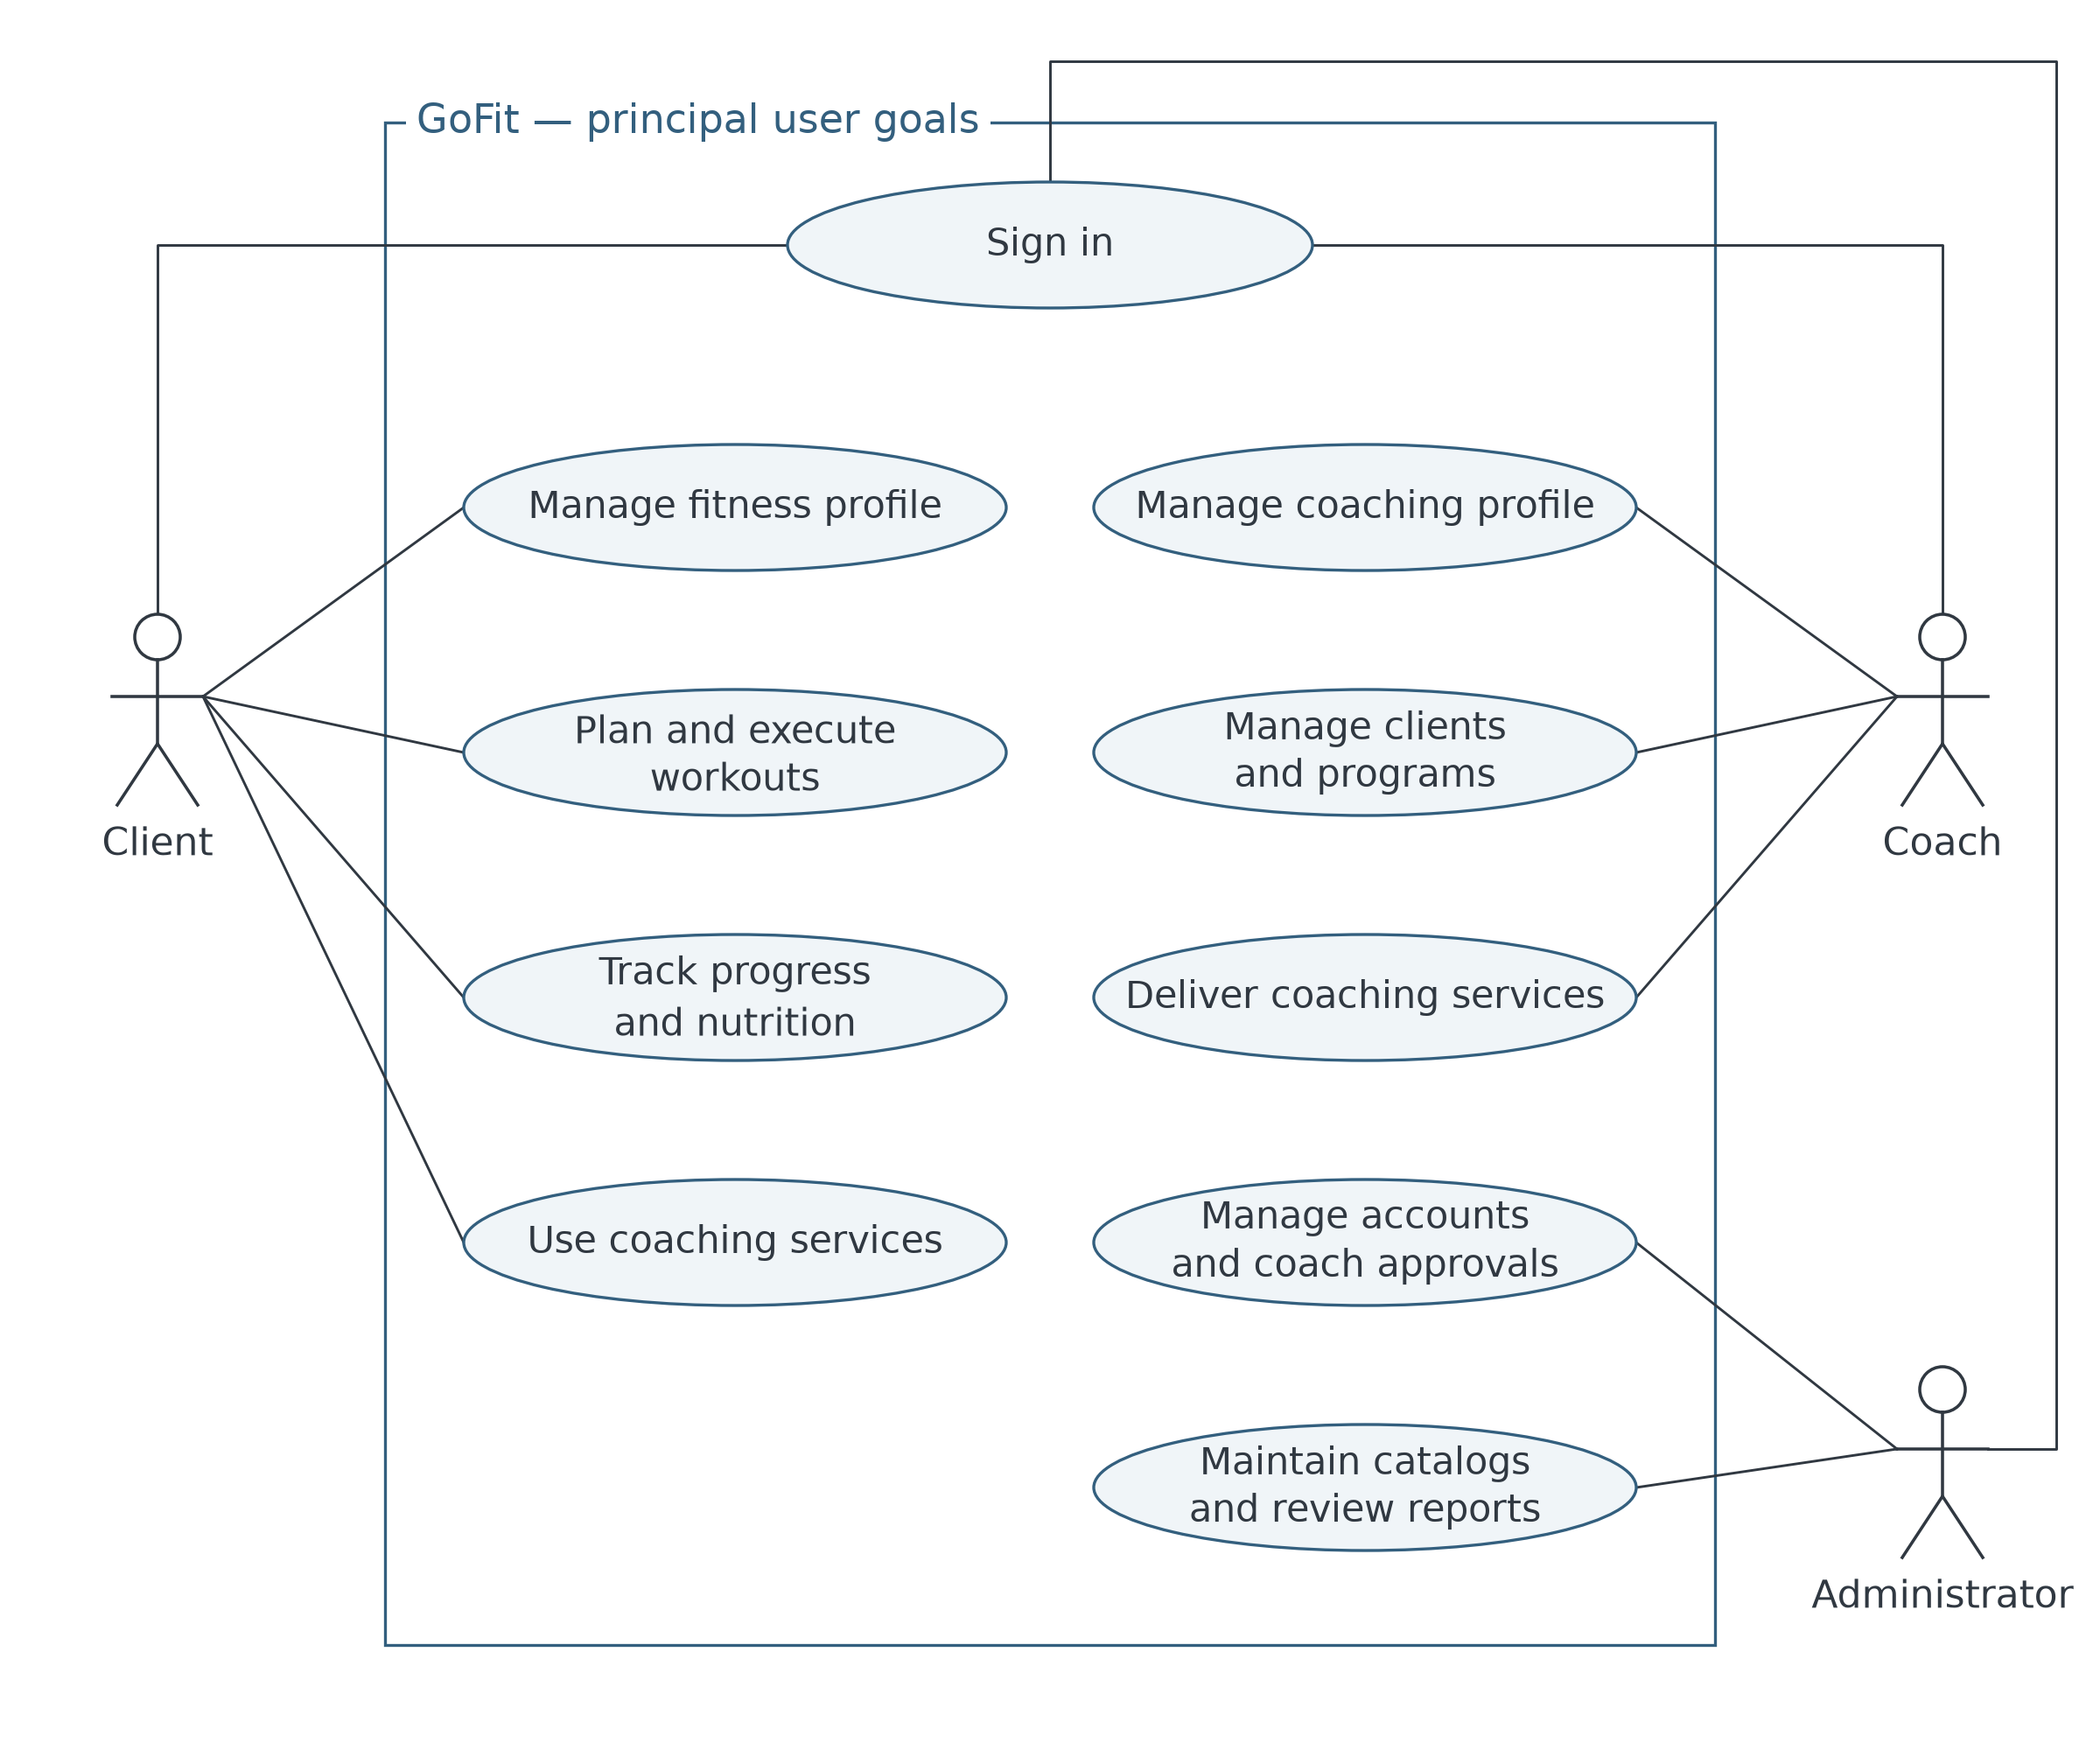
\includegraphics[width=0.95\linewidth]{figures/global_use_case.png}
\caption{Principal user goals of the GoFit platform}
\label{fig:global_use_case}
\end{figure}

\section{Project Management}

The project was managed through a backlog and sprint-based organization. Technical work was divided between the mobile app, web admin panel, database migrations, backend functions, documentation, testing, and deployment preparation. The repository structure itself supports this organization through separate folders for GoFitMobile, admin-panel, database, and docs.


The project management approach also included technical documentation as a project artifact, not as an afterthought. The repository contains architecture notes, feature inventories, sprint breakdowns, troubleshooting reports, database structure documentation, admin-panel notes, body-measurement research, validation protocols, and automation workflow descriptions. This documentation helped connect implementation choices to report sections and made it possible to justify complex AI and backend decisions.


Table \ref{tab:pdf-27-15} lists the documentation artifacts maintained during the project. Each artifact is described by its purpose and the information it captures, which shows that documentation was treated as an integral part of project management.


\begingroup
\footnotesize
\setlength{\tabcolsep}{3pt}
\renewcommand{\arraystretch}{1.20}
\setlength{\LTpre}{5pt}
\setlength{\LTpost}{10pt}
\begin{longtable}{|L{3.67cm}|L{5.29cm}|L{5.73cm}|}
\caption{Project documentation artifacts}\label{tab:pdf-27-15} \\
\hline
Artifact type & Purpose in the project & Examples of information captured \\ \hline
Architecture documentation & Explains the global system structure and deployment view. & Mobile app, admin panel, Supabase backend, Edge Functions, external services, diagrams. \\ \hline
Feature inventory & Lists implemented screens, services, routes, functions, and database artifacts. & Client features, coach features, admin features, backend functions, migrations, integrations. \\ \hline
Sprint and Gantt documentation & Records alternative planning schedules; not a completed execution log. & January--July dates, differing iteration schemes, objectives, dependencies and planned release activities. \\ \hline
AI research notes & Records model decisions, tests, limitations, and validation needs. & MoveNet, MediaPipe Pose Landmarker, segmentation models, feature vectors, statistical estimator. \\ \hline
Automation documentation & Explains scheduled and event-driven backend workflows. & n8n AI session preparation, admin operations digest, notification creation. \\ \hline
Academic/report drafts & Transforms engineering material into PFE reporting structure. & Problem statement, methodology, report plan, diagram drafts, bibliography entries. \\ \hline
\end{longtable}
\endgroup

\phantomsection
\section*{Conclusion}

This chapter defined the actors, requirement targets, backlog priorities and principal user goals used to structure GoFit. The internship interval is confirmed, while exact mapping between the planning iterations and report scope groups remains unverified. The next chapter examines the mobile foundation and workout paths under the Sprint 1 heading.


\chapter{Sprint 1}


\phantomsection
\section*{Introduction}
\addcontentsline{toc}{section}{Introduction}

Sprint 1 addresses the GoFit foundational core: mobile project architecture, Supabase GoTrue authentication, multi-screen client onboarding, profile management, workout template building, active workout session logging, and rest timing. The current onboarding navigator registers six screens: introduction, weight, height, personal details, goal, and nutrition preferences. Local onboarding completion is distinct from successful remote profile persistence, as examined in the authentication sequence analysis.


This chapter examines the scope designated Sprint 1 through planned tasks, cumulative domain views, selected use cases and interaction sequences, implementation descriptions and reconciled validation criteria. The models project the inspected implementation, while the retained October observations are later evidence. The closing management subsection states the limits of available progress-tracking data.


\section{Needs Assessment}

The sprint needs were selected from the prioritized product backlog according to dependency order, business value, and architectural feasibility. The following table provides a comprehensive decomposition of each user story into technical modeling, implementation, and testing subtasks.


The sprint objective is to provide authenticated access, profile onboarding, workout planning and execution, and configurable rest timing. The backlog below states development and testing targets; inclusion of a task does not establish its completion or a successful test result.


\subsection{Sprint Backlog}


\begingroup
\scriptsize
\setlength{\tabcolsep}{3pt}
\renewcommand{\arraystretch}{1.20}
\setlength{\LTpre}{5pt}
\setlength{\LTpost}{10pt}
\begin{longtable}{|L{1.00cm}|L{0.95cm}|L{4.80cm}|L{1.20cm}|L{6.20cm}|L{1.60cm}|}
\caption{Sprint 1 backlog decomposition}\label{tab:pdf-29-16} \\
\hline
\rowcolor{entetetab}
ID US & As & User Story & Id task & Task & Estimation (pts) \\ \hline
\endfirsthead
\hline
\rowcolor{entetetab}
ID US & As & User Story & Id task & Task & Estimation (pts) \\ \hline
\endhead
US-3.1 & User & Create account, log in securely, and complete 4-step onboarding questionnaire (goals, experience, equipment) & T3.1.1 & Model UserProfile schema, Supabase Auth GoTrue JWT integration, and onboarding state machine. & 3 \\ \hline
US-3.1 & User & Create account, log in securely, and complete 4-step onboarding questionnaire (goals, experience, equipment) & T3.1.2 & Implement AuthScreen, OnboardingScreen with multi-step questionnaire, and Zustand authStore. & 5 \\ \hline
US-3.1 & User & Create account, log in securely, and complete 4-step onboarding questionnaire (goals, experience, equipment) & T3.1.3 & Test GoTrue authentication, token refresh in SecureStore, and protected navigation redirection. & 3 \\ \hline
US-3.2 & User & Browse workout templates, customize exercise parameters, and create personal workouts & T3.2.1 & Design Workout, Exercise, and WorkoutExercise entity relationship model in Supabase. & 3 \\ \hline
US-3.2 & User & Browse workout templates, customize exercise parameters, and create personal workouts & T3.2.2 & Develop WorkoutListScreen, WorkoutDetailScreen, and WorkoutBuilderScreen with reorderable exercises. & 5 \\ \hline
US-3.2 & User & Browse workout templates, customize exercise parameters, and create personal workouts & T3.2.3 & Verify workout template cloning, custom exercise creation, and Zustand workoutStore state sync. & 3 \\ \hline
US-3.3 & User & Execute an active workout session with set logging (weight, reps, RPE) and an animated rest timer & T3.3.1 & Model WorkoutSession and WorkoutSet tables with offline persistence support. & 5 \\ \hline
US-3.3 & User & Execute an active workout session with set logging (weight, reps, RPE) and an animated rest timer & T3.3.2 & Implement WorkoutSessionScreen with set completion checkboxes, audio/haptic rest timer, and auto-advance. & 8 \\ \hline
US-3.3 & User & Execute an active workout session with set logging (weight, reps, RPE) and an animated rest timer & T3.3.3 & Test timer background execution, haptic vibration alerts, and set metric calculations. & 3 \\ \hline
US-3.4 & User & Persist workout history and offline session data with automatic synchronization to Supabase & T3.4.1 & Design SQLite/AsyncStorage offline queue schema with conflict resolution timestamps. & 5 \\ \hline
US-3.4 & User & Persist workout history and offline session data with automatic synchronization to Supabase & T3.4.2 & Implement WorkoutService offline sync queue and Supabase database mutations. & 5 \\ \hline
US-3.4 & User & Persist workout history and offline session data with automatic synchronization to Supabase & T3.4.3 & Validate network failure recovery, auto-retry on reconnection, and Supabase RLS row insertion. & 3 \\ \hline
\end{longtable}
\endgroup

The backlog is retained as a planning artifact, including its original task identifiers and estimates. The cumulative model and sequences describe the inspected implementation rather than a dated sprint-end snapshot. US-3.2 maps to the Workout--WorkoutExercise--Exercise prescription model; a complete reorder or cloning workflow is not established by the retained QA. US-3.3 maps to WorkoutSession and embedded SessionExerciseSnapshot values, not a persisted WorkoutSet entity. US-3.4 maps to the conditional offline completion sequence, not unrestricted offline creation. Table~\ref{tab:sprint-traceability} connects these deviations and the remaining sprint stories to the evidence matrix.

\subsection{Sprint Class Diagram}

The backlog records targets whose wording differs from the current implementation. US-3.1's four-step questionnaire is superseded in the inspected navigator by the six-screen flow described above. US-3.3's RPE input and separate WorkoutSet table are not implemented in the inspected session path: weights and completion flags are recorded with configured repetitions in embedded session snapshots. For US-3.4, the implemented queue uses AsyncStorage through a separate offline queue service, with application connectivity handling retrying completion updates to an existing remote session. These paths do not establish SQLite persistence, timestamp conflict resolution, or unrestricted offline session creation. The listed testing tasks remain targets until supported by execution evidence.

The Sprint 1 domain model distinguishes the authentication account from its optional fitness profile and represents the principal workout definitions and execution records. Native and custom workouts share a common Workout concept; only custom workouts have a personal owner. WorkoutExercise associates an exercise with its prescribed sets, repetitions, rest interval, day, and order. A WorkoutSession belongs to an account and may optionally reference a workout definition. Profile measurements may remain unset, while completion timestamps and durations are optional for ongoing sessions. Session exercise data are retained as embedded snapshots containing exercise information, completion flags, and recorded weights, rather than as independently persisted WorkoutSet entities. Rest-timer preferences are represented separately as local application configuration. Services, stores, and synchronization mechanisms are described in the technical interaction diagrams.


\begin{figure}[H]
\centering
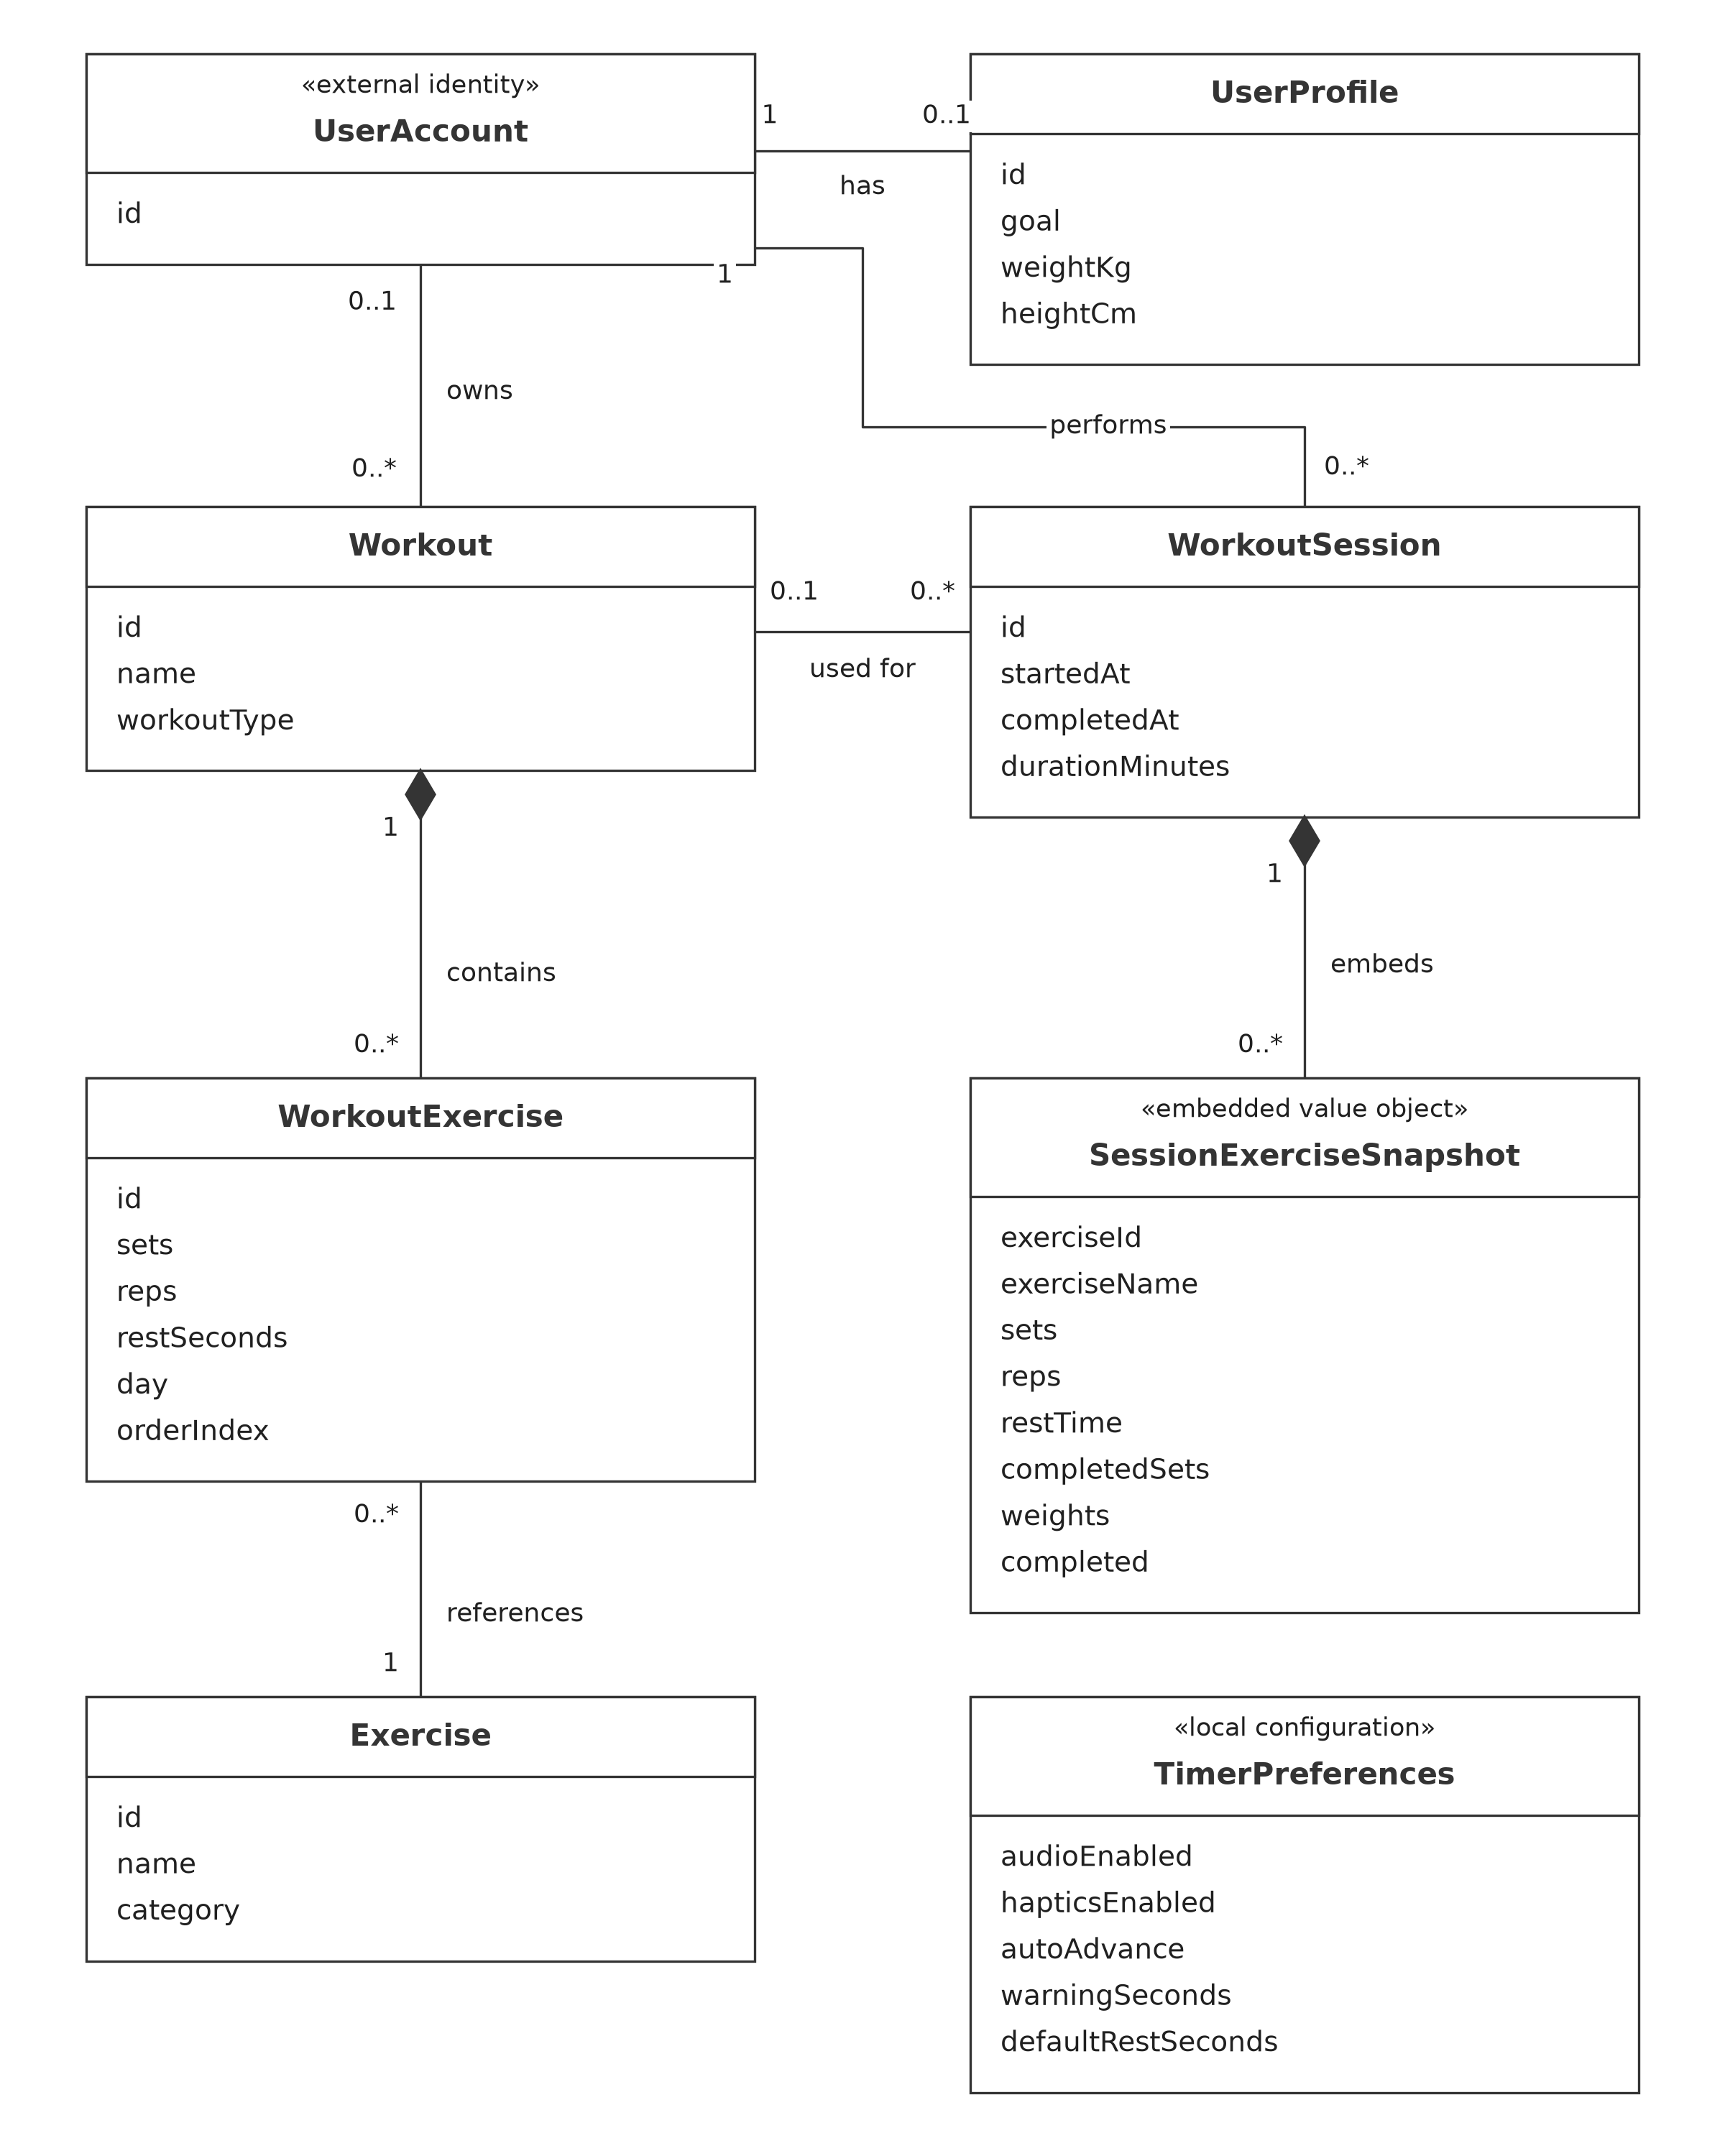
\includegraphics[width=0.95\linewidth]{figures/class_diagram_sprint1.png}
\caption{Sprint 1 structural domain class diagram}
\label{fig:class_sprint1}
\end{figure}

\section{Functional Specification of Requirements}

This section specifies the sprint use cases and analyzes the behavioral interactions between the participating actors and the GoFit platform.


\subsection{Refined Use Case Diagram of Sprint 1}

The Client is the primary actor in this view. The selected goals cover registration and sign-in, client onboarding, fitness-profile management, workout browsing and creation, workout execution, and rest-timer configuration. Recording set information and using the timer occur within workout execution. Queuing a failed completion update for an existing session is a conditional implementation path, described in the sequence analysis, rather than a separate user goal.


\begin{figure}[H]
\centering
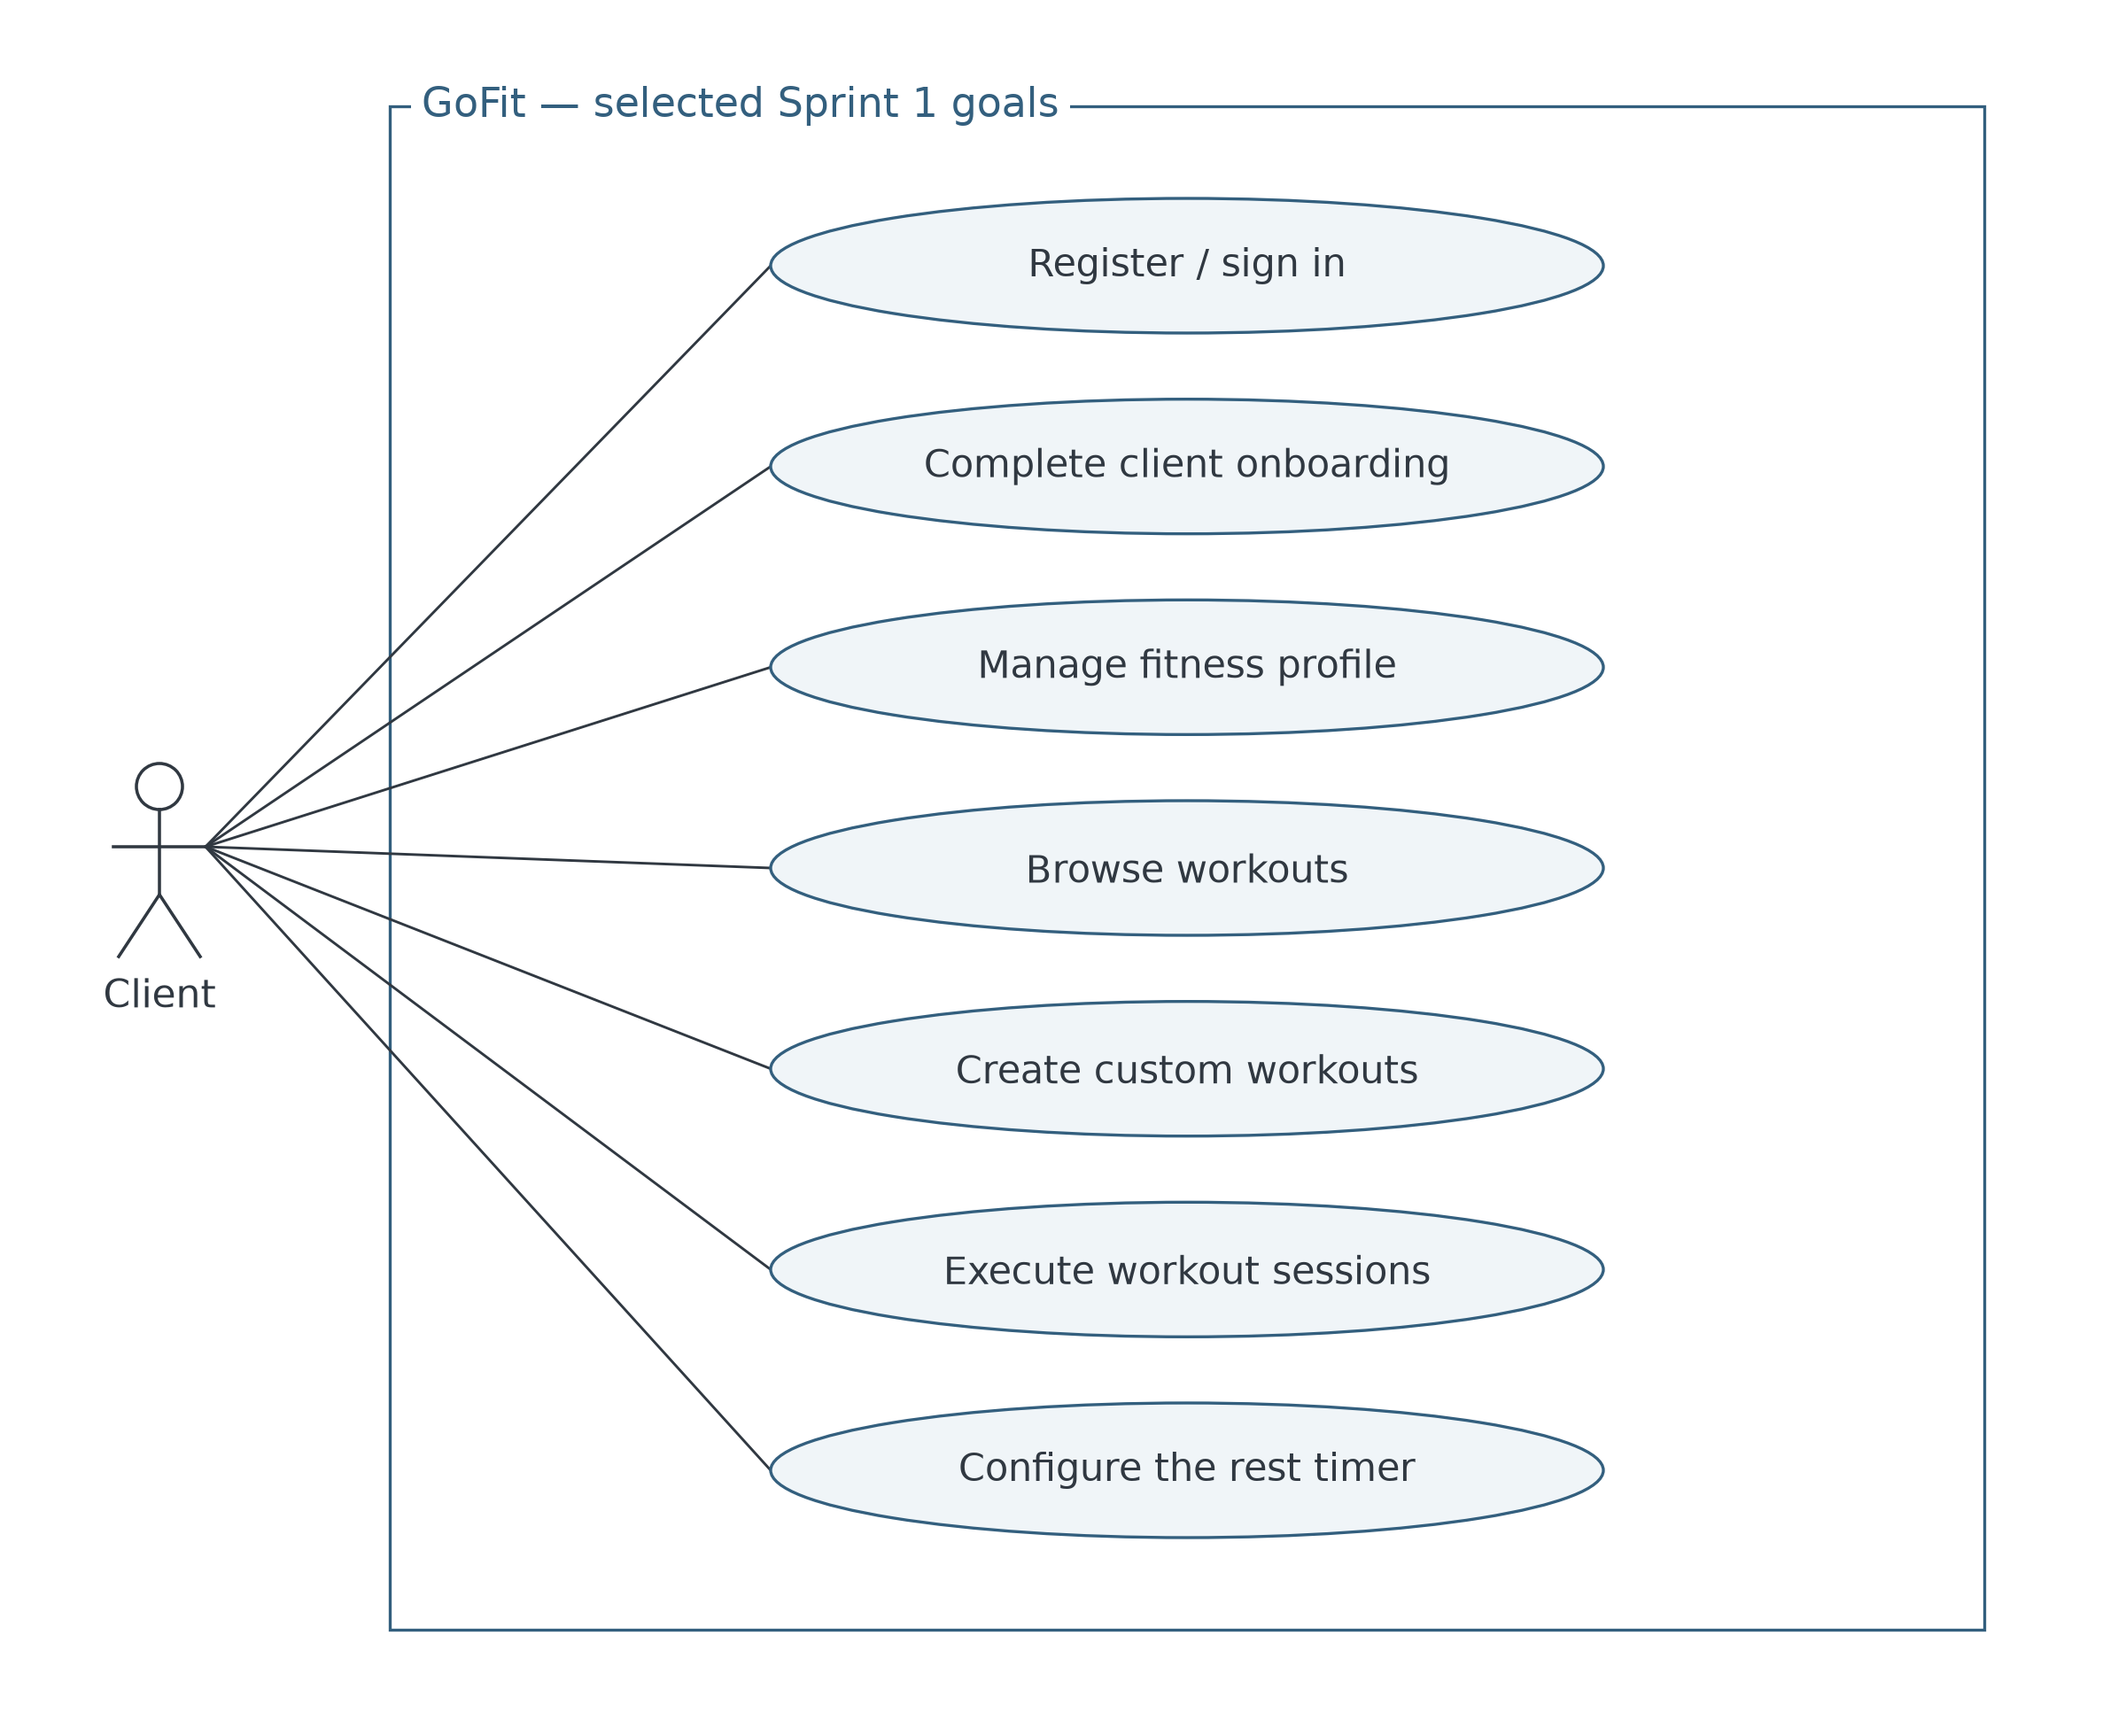
\includegraphics[width=0.92\linewidth]{figures/use_case_sprint1.png}
\caption{Selected client use cases associated with Sprint 1}
\label{fig:use_case_sprint1}
\end{figure}

\subsection{Use Case Analysis}

\subsubsection{Use case: Execute workout session}

\begingroup
\footnotesize
\setlength{\tabcolsep}{3pt}
\renewcommand{\arraystretch}{1.20}
\setlength{\LTpre}{5pt}
\setlength{\LTpost}{10pt}
\begin{longtable}{|L{4.95cm}|L{10.05cm}|}
\caption{Textual description of use case: Execute workout session}\label{tab:pdf-34-17} \\
\hline
\rowcolor{entetetab}
Field & Description \\ \hline
\endfirsthead
\hline
\rowcolor{entetetab}
Field & Description \\ \hline
\endhead
Use case & Execute workout session \\ \hline
Primary actor & Mobile user \\ \hline
Preconditions & The user is authenticated and a workout template or custom workout exists. \\ \hline
Postconditions & On successful remote completion, the existing workout session is updated with completion time, duration, exercise snapshots, and optional feedback notes. If completion is queued successfully while disconnected, the remote update remains pending. \\ \hline
Nominal scenario & 1. The user selects a workout and reviews its configured exercises, sets, and repetitions. 2. The user starts the workout; the system creates a session and retains its identifier. 3. The user enters set weights and marks sets as complete. 4. The system updates local progress, gives completion haptic feedback, and displays a rest countdown. 5. The user selects Finish Workout and submits optional difficulty feedback and notes. 6. The system updates the existing session, then displays a summary with duration, completed sets, and volume calculated from recorded weights and configured repetitions. \\ \hline
Alternative scenario & 3.1. The user can undo a set-completion mark or pause the session. 4.1. The user can skip the rest countdown. 6.1. If the completion update fails and the connectivity check reports disconnection, the screen queues an update for the already-created session in AsyncStorage. After a successful local write, it displays an offline-save message and the summary. A later connectivity event handled by the application triggers synchronization. \\ \hline
Exception scenario & E.1. Session creation fails; the system displays an error and does not start the session. E.2. Completion fails while the connectivity check reports a connection; the system displays a save error. E.3. Local queue persistence fails; the system displays a retry message, without confirming a successful save. \\ \hline
\end{longtable}
\endgroup

\begin{figure}[H]
\centering
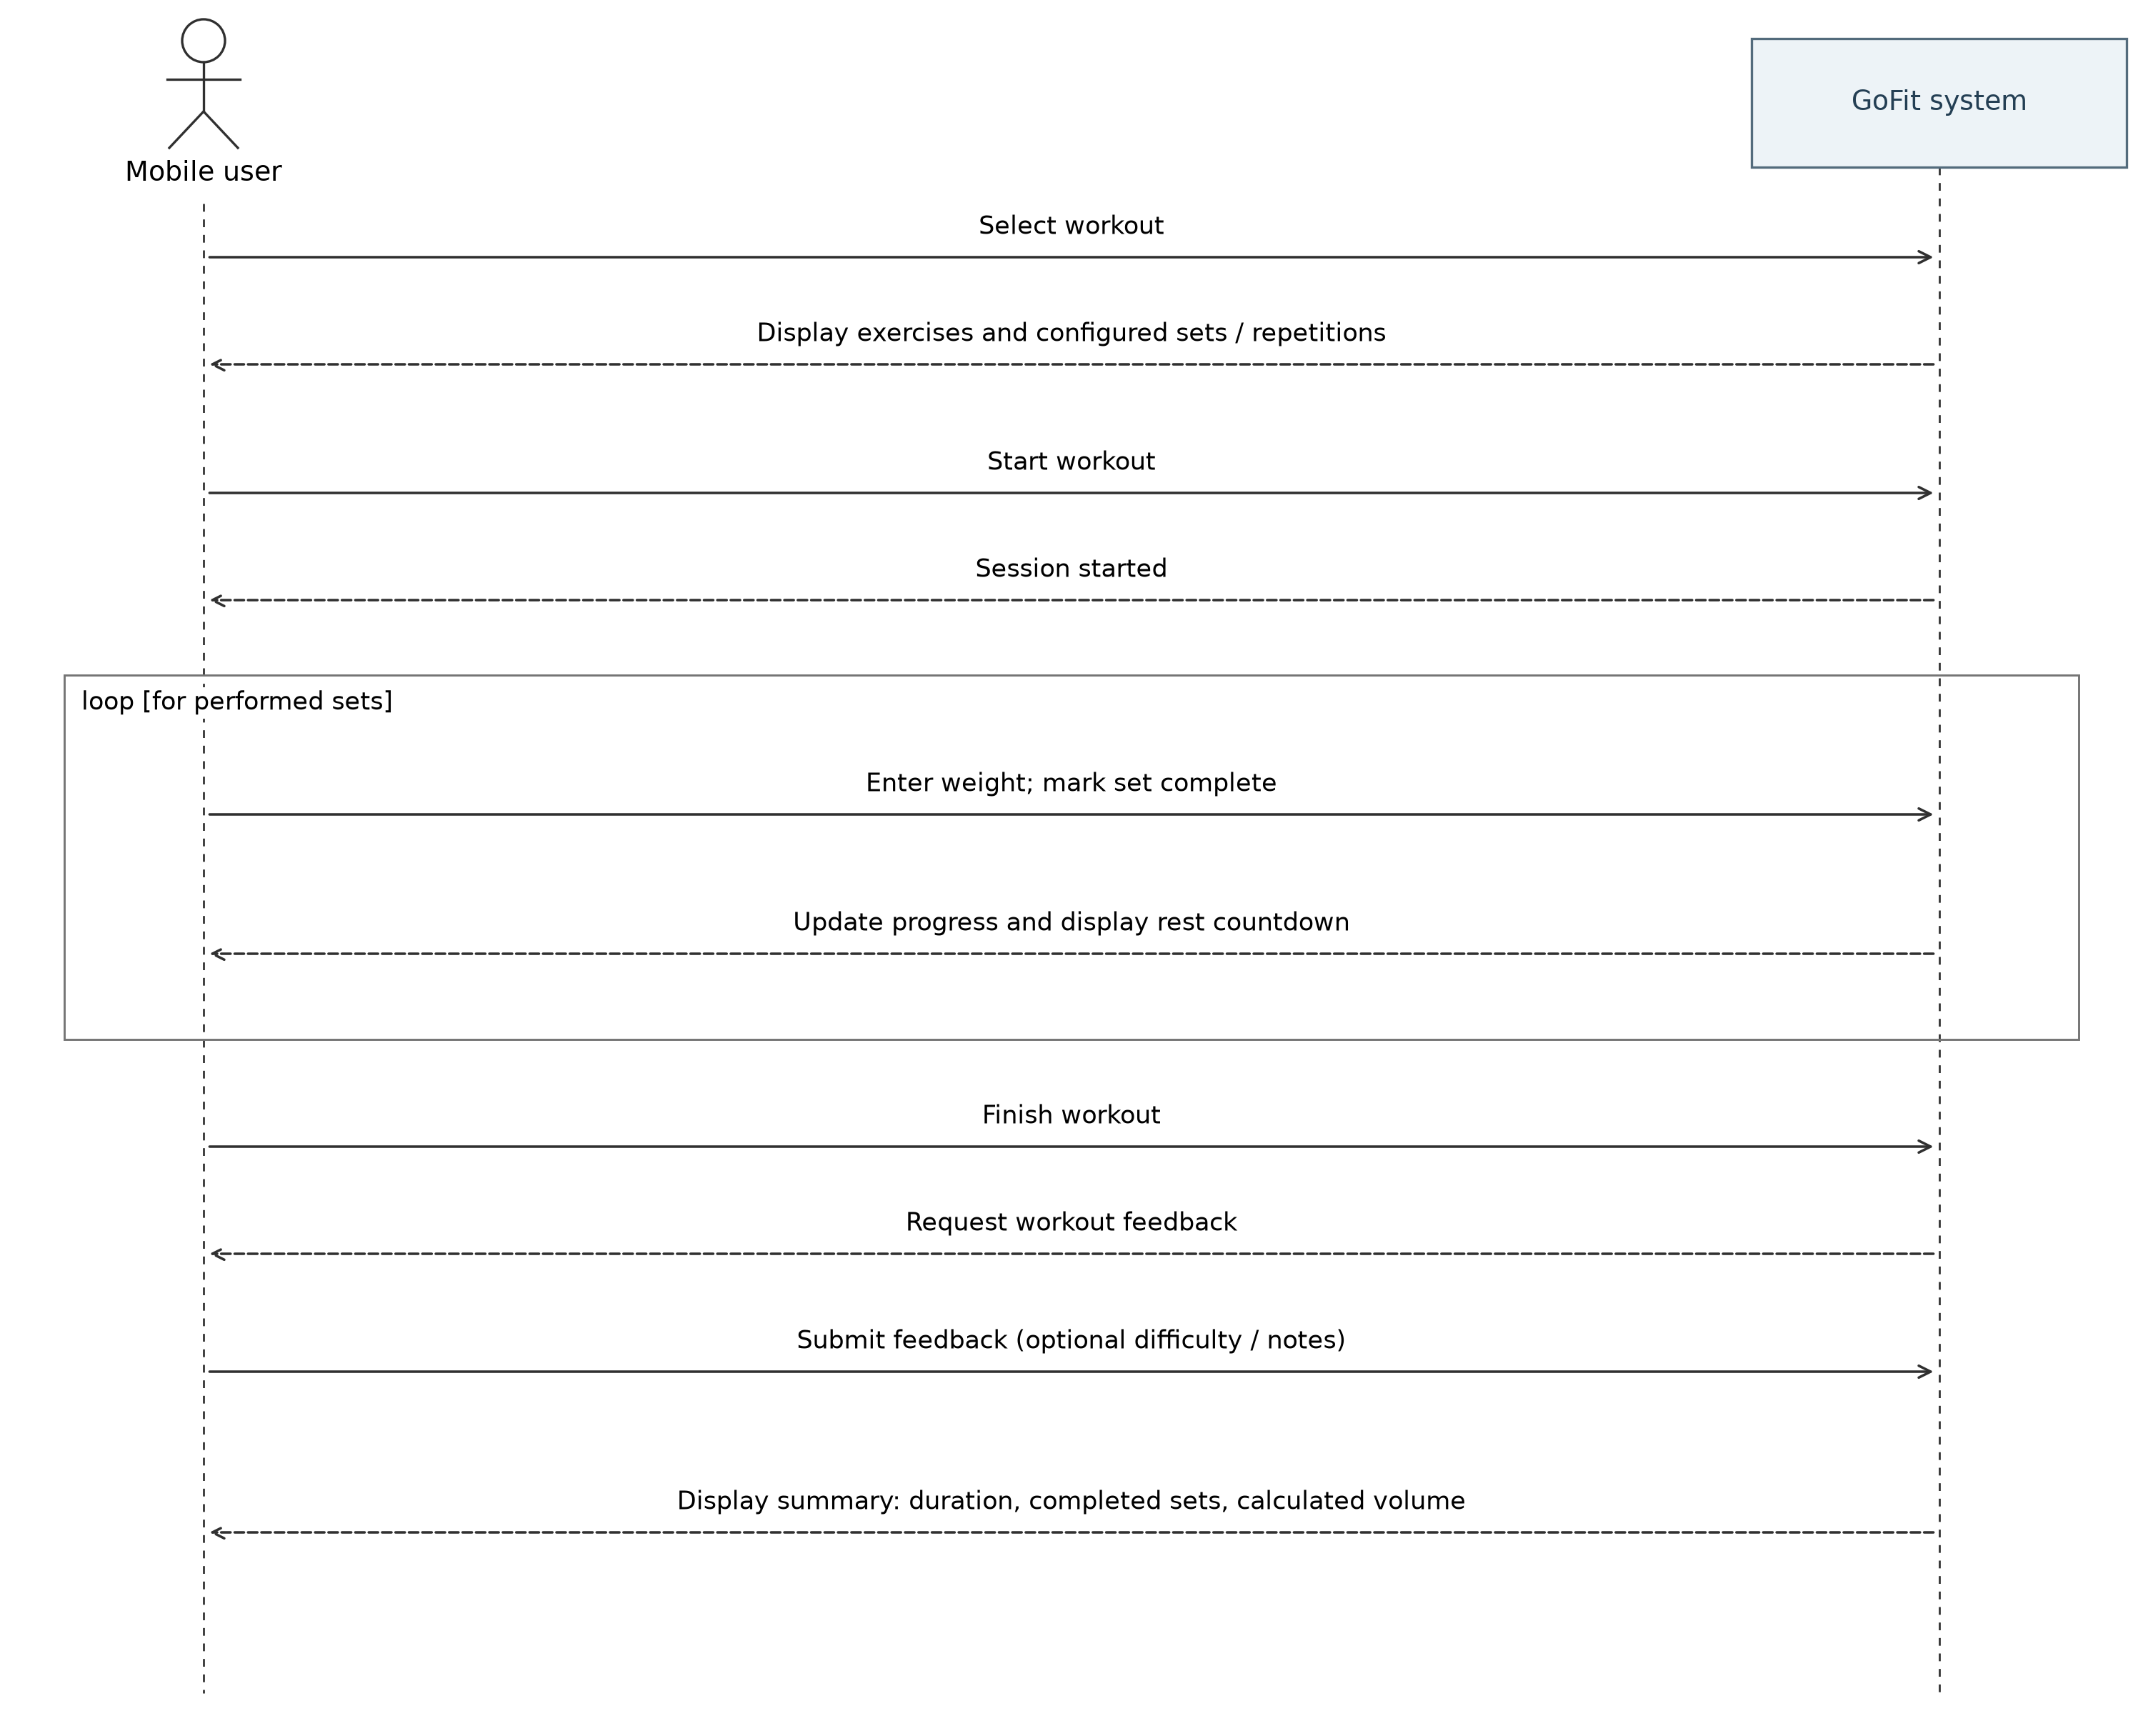
\includegraphics[width=0.92\linewidth]{figures/seq_workout_ssd.png}
\caption{System sequence diagram: Execute workout session, successful online path}
\label{fig:seq_workout_ssd}
\end{figure}

\begin{figure}[H]
\centering
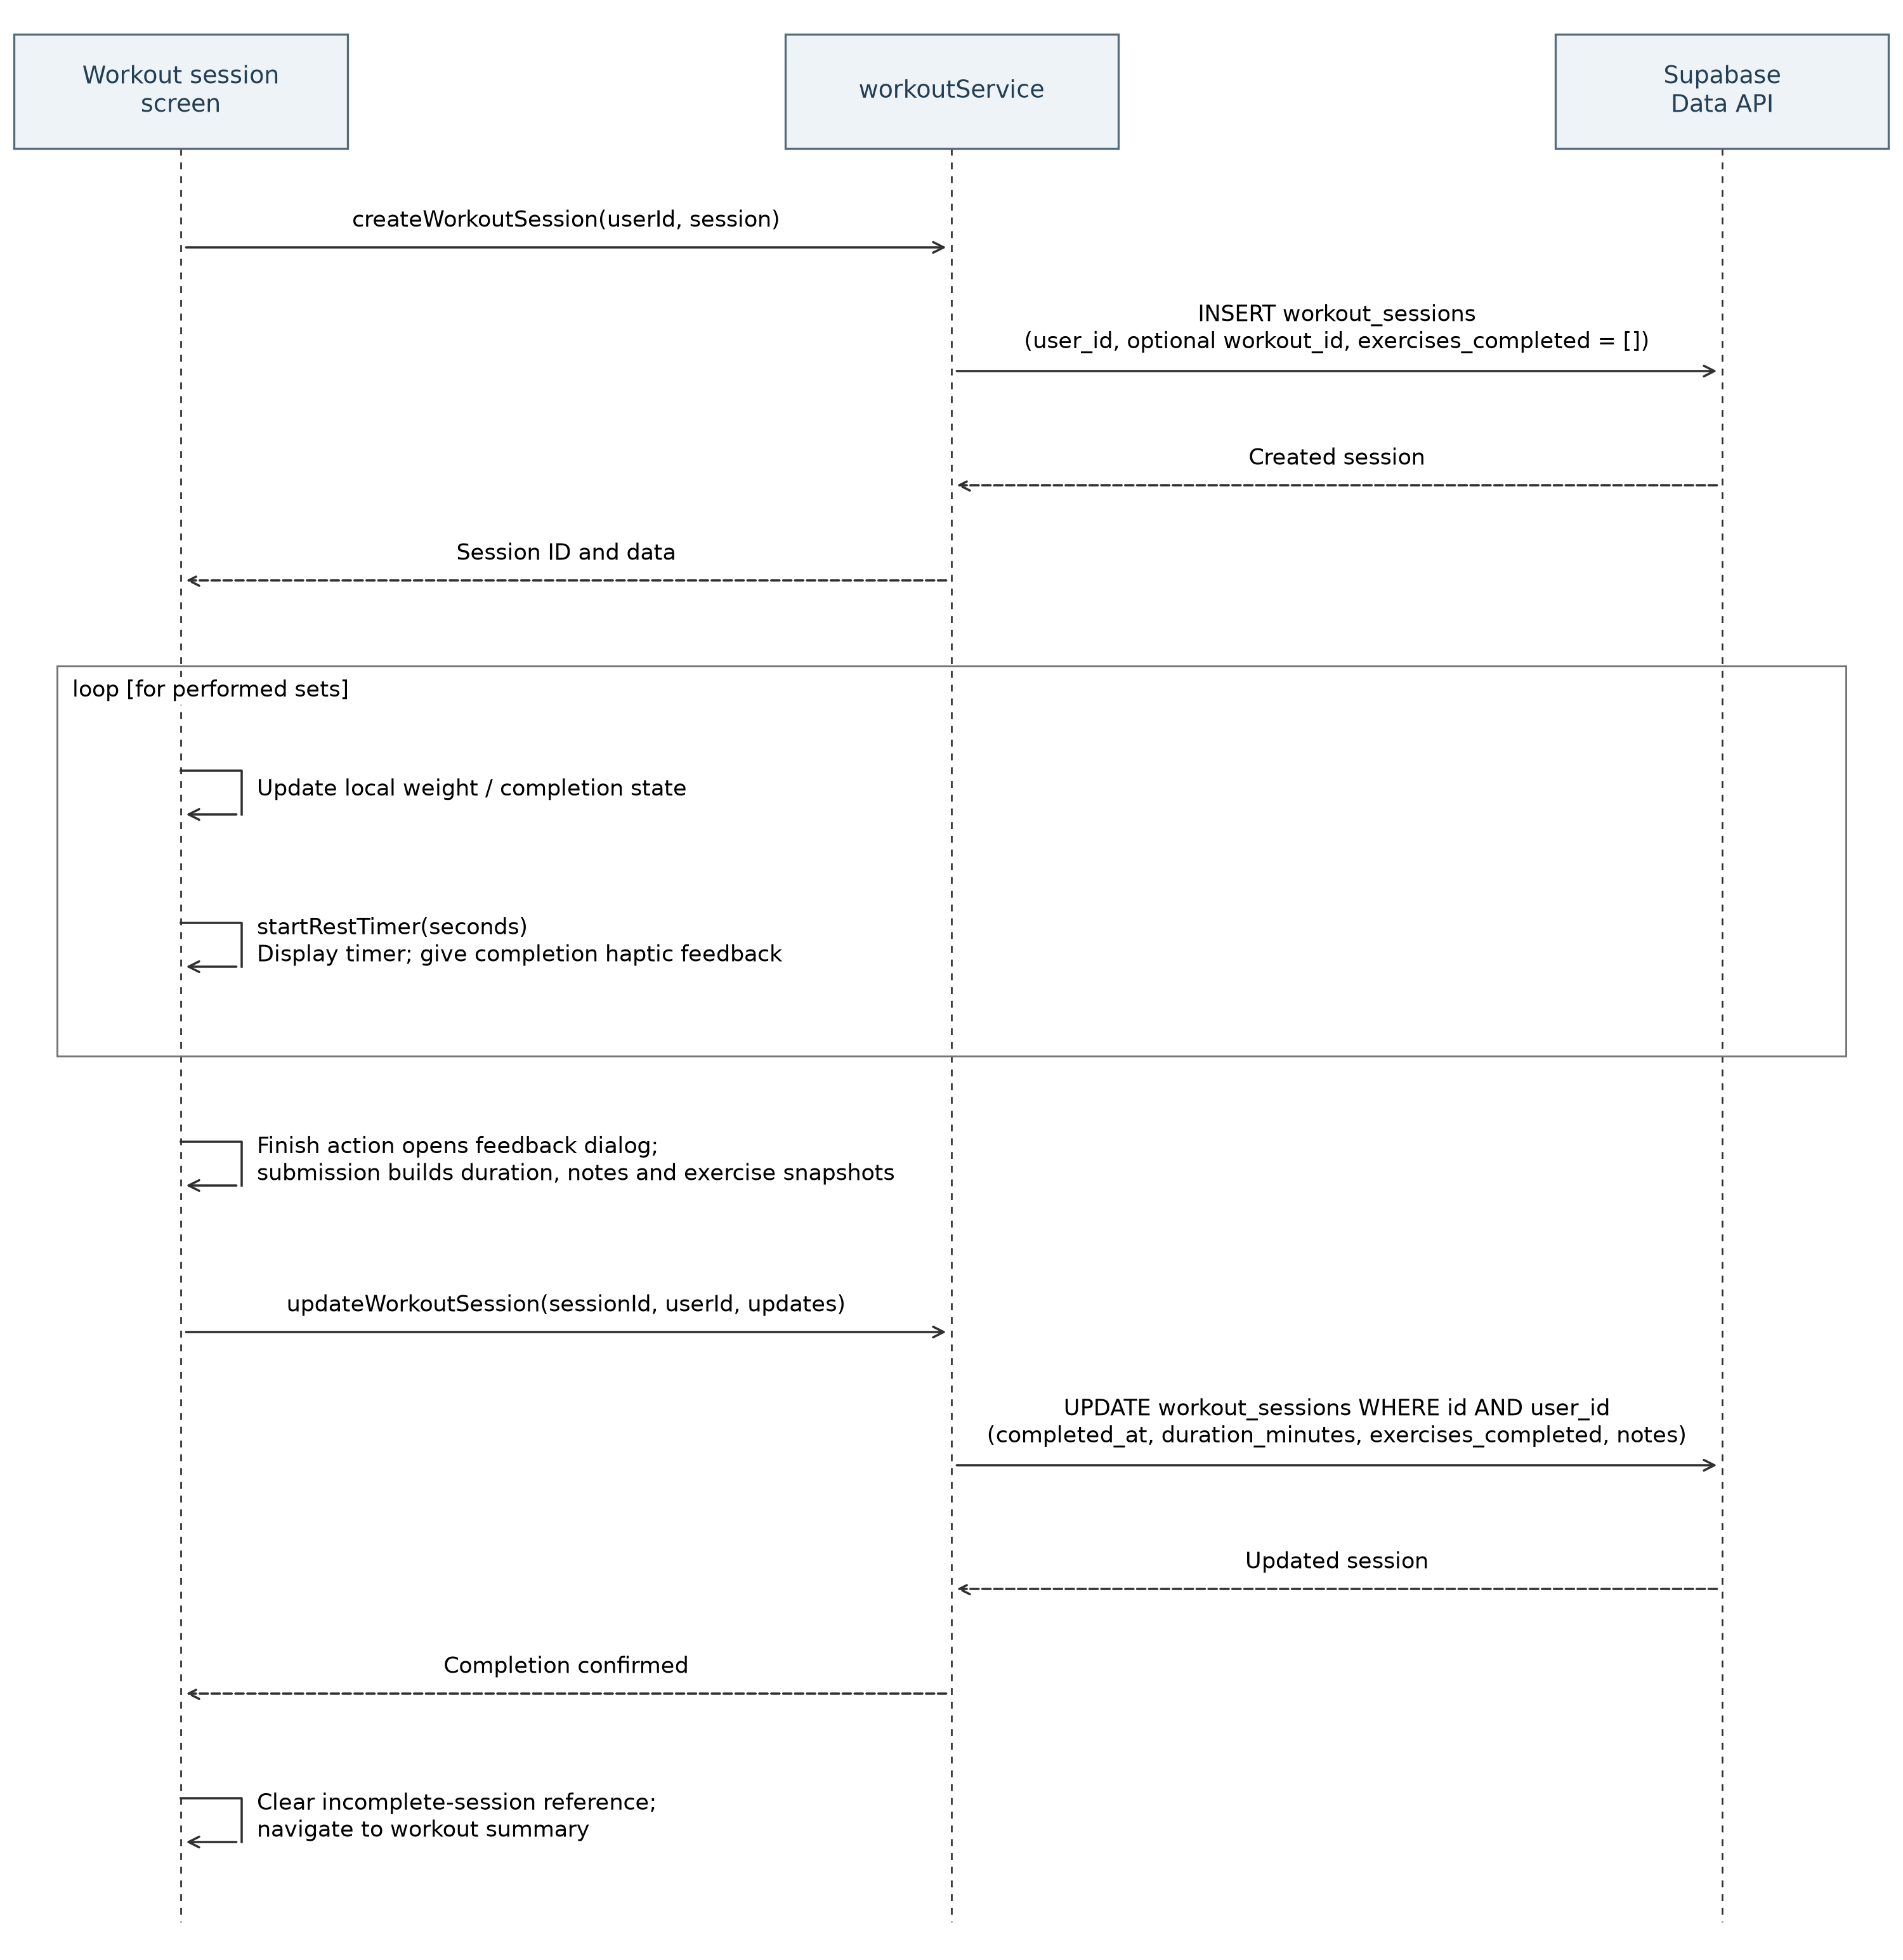
\includegraphics[width=0.92\linewidth]{figures/seq_workout_detailed.png}
\caption{Technical sequence diagram: Session creation and successful online completion}
\label{fig:seq_workout_detailed}
\end{figure}

Figures~\ref{fig:seq_workout_ssd} and~\ref{fig:seq_workout_detailed} present the successful online path for a new workout session. The technical view selects the core creation, execution, and completion interactions; exercise retrieval, optional calendar updates, and intermediate progress saves are omitted. The screen calls the workout service through the configured Supabase client and Data API, rather than connecting directly to PostgreSQL. Session creation inserts a row into \texttt{workout\_sessions}; the service first checks for an earlier incomplete session and, if found, attempts to mark it completed. Creation must succeed before the execution flow proceeds. The screen then manages exercise progress and rest-timer state locally. The workout store supports incomplete-session references rather than performing each set update. Completion updates the existing row with \texttt{completed\_at}, \texttt{duration\_minutes}, notes, and the embedded \texttt{exercises\_completed} collection. No separate set-table insertion is performed by this path. Summary volume uses configured repetitions and entered weights for sets marked complete; it is not an independent measurement of repetitions performed.

\begin{figure}[H]
\centering
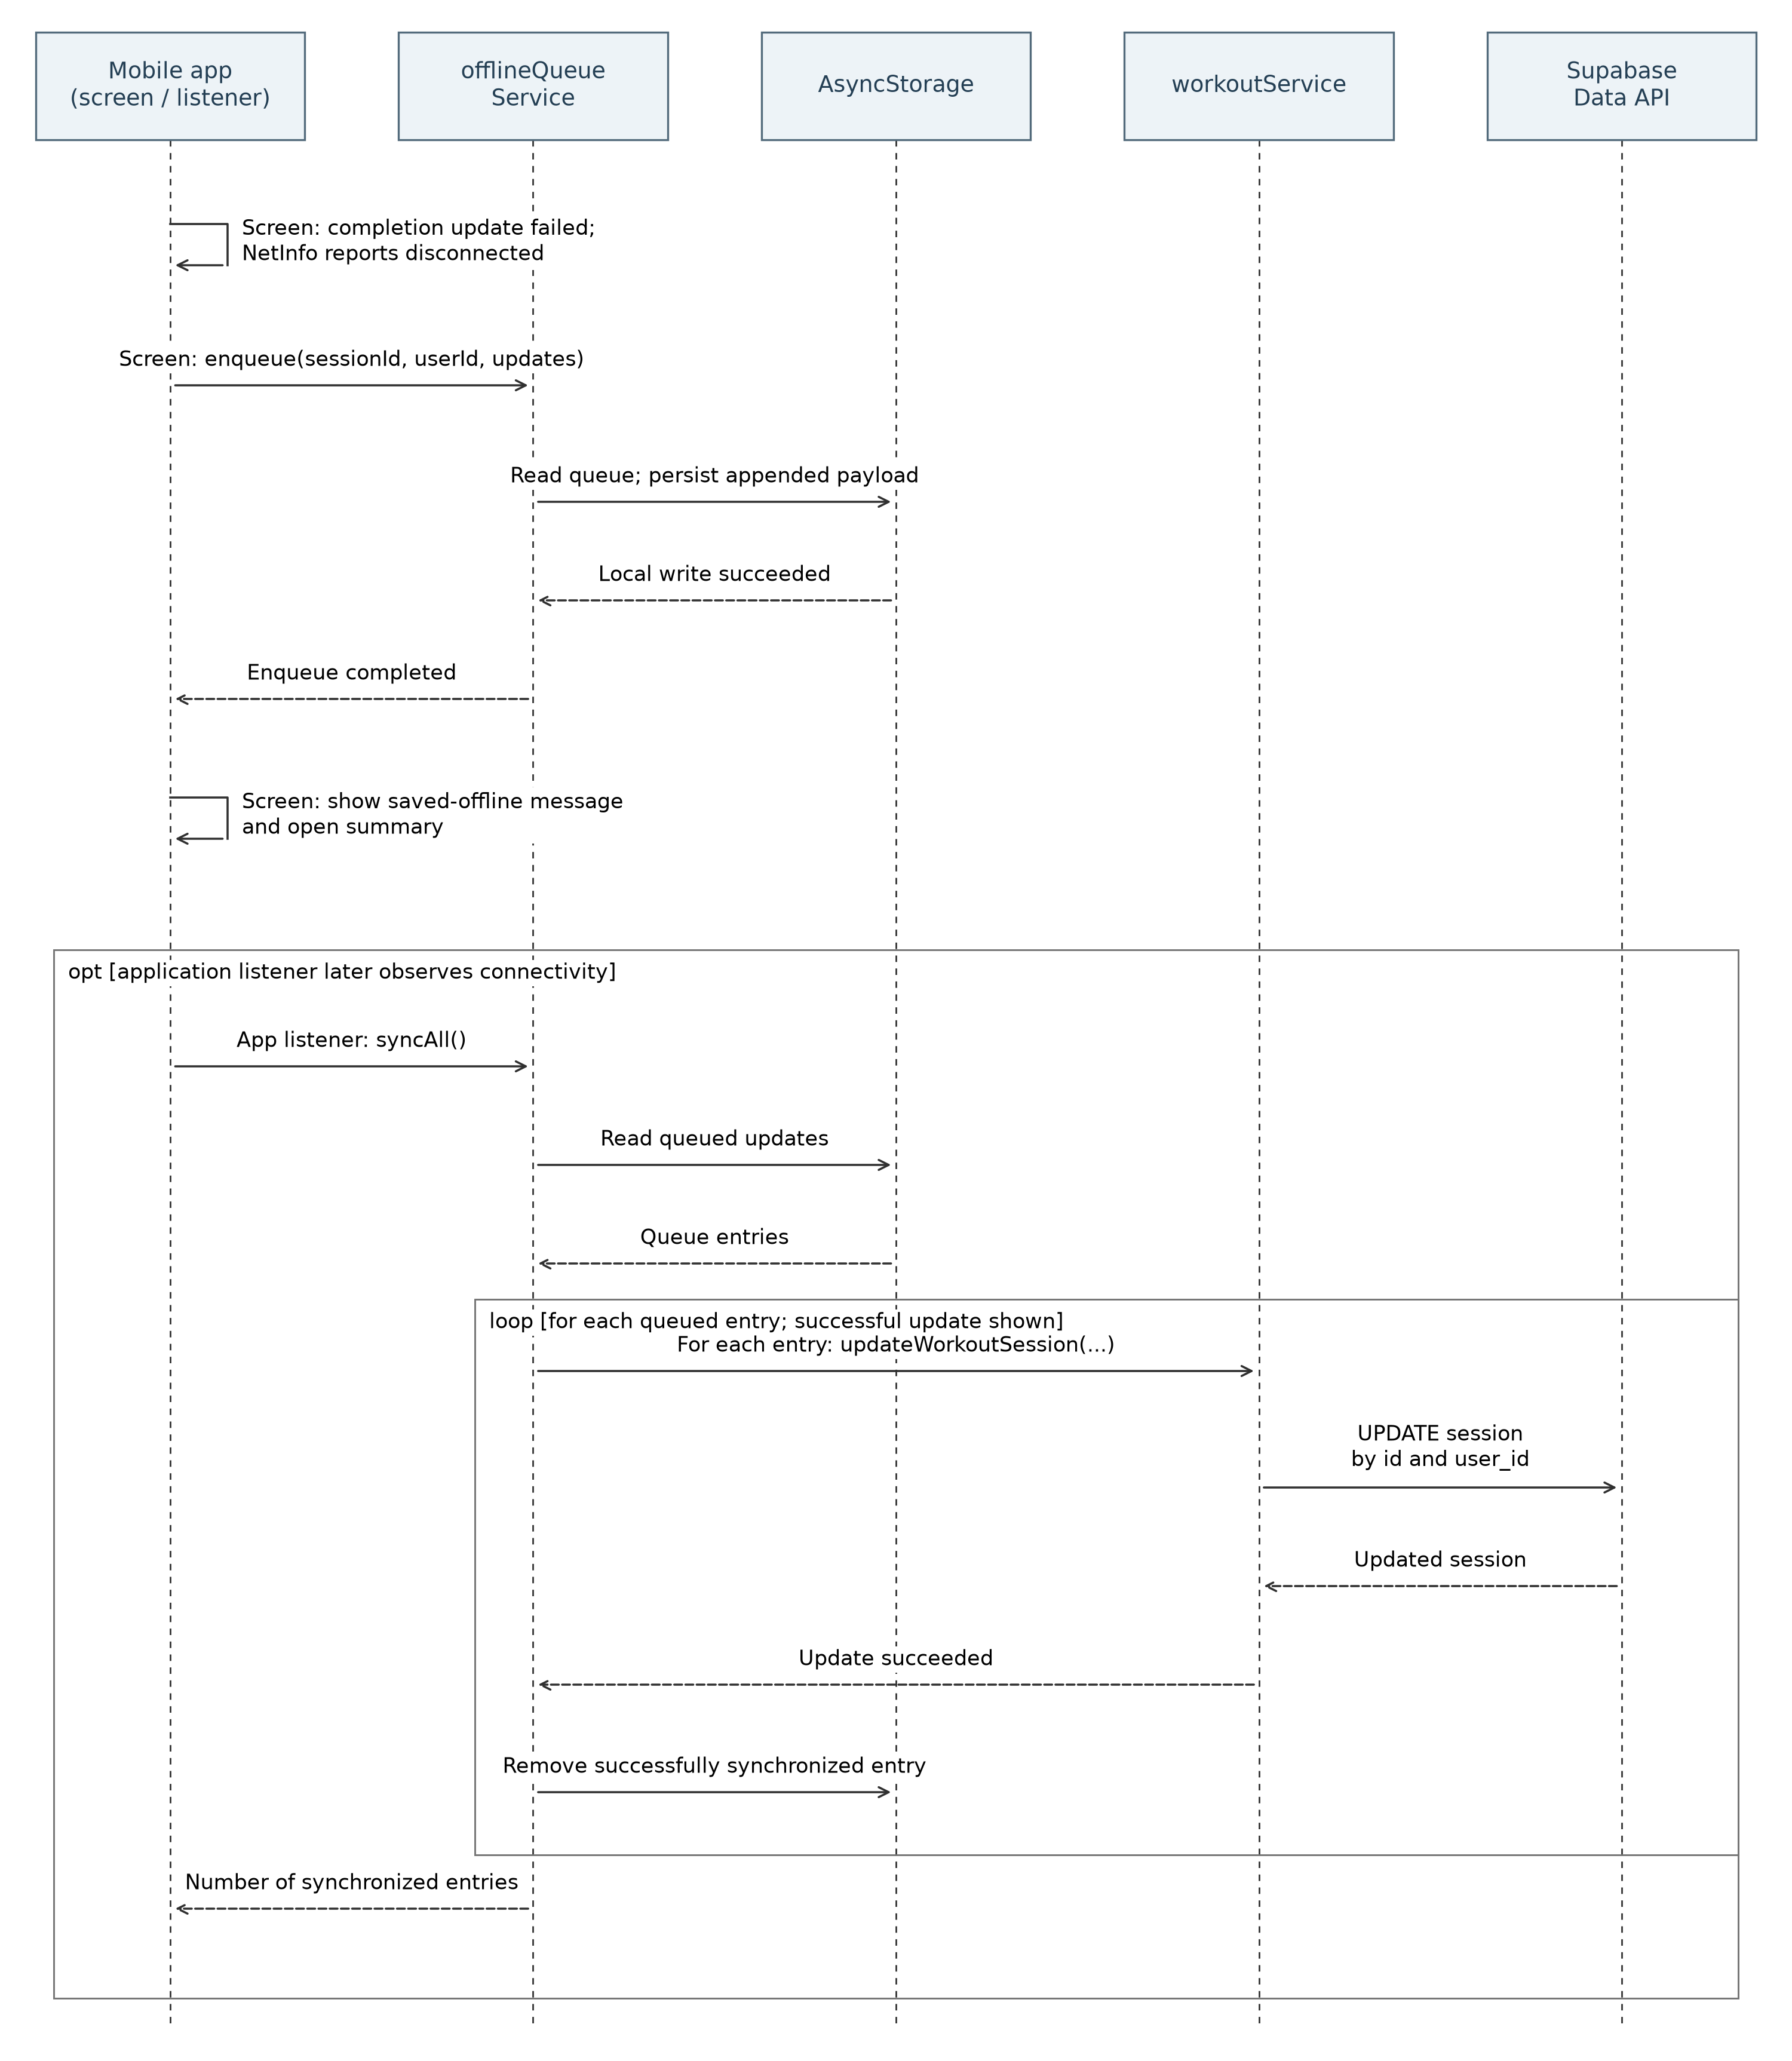
\includegraphics[width=0.95\linewidth]{figures/seq_workout_offline.png}
\caption{Technical sequence diagram: Offline completion and later successful synchronization}
\label{fig:seq_workout_offline}
\end{figure}

Figure~\ref{fig:seq_workout_offline} details the disconnected completion alternative for a session that already has a remote identifier. Following a failed update, the screen checks connectivity with NetInfo and, when disconnected, calls the offline queue service. The diagram groups the screen and the application's connectivity listener within one mobile-application lifeline; the message labels identify each caller. A successful AsyncStorage write permits the screen to show the summary while remote persistence remains pending. When the application's listener later observes connectivity, \texttt{syncAll()} checks the connection, reads the queue, and retries each session update through the workout service. Successfully synchronized entries are removed; entries whose remote update fails remain queued for a subsequent attempt. This application-level retry mechanism does not establish execution while the application is terminated, entirely offline session creation, or guaranteed protection against storage failure. The offline payload preserves written feedback notes but currently omits the difficulty prefix included by the online completion path.


\subsubsection{Use case: Authenticate and complete onboarding}

\begingroup
\footnotesize
\setlength{\tabcolsep}{3pt}
\renewcommand{\arraystretch}{1.20}
\setlength{\LTpre}{5pt}
\setlength{\LTpost}{10pt}
\begin{longtable}{|L{4.95cm}|L{10.05cm}|}
\caption{Textual description of use case: Authenticate and complete onboarding}\label{tab:pdf-37-18} \\
\hline
\rowcolor{entetetab}
Field & Description \\ \hline
\endfirsthead
\hline
\rowcolor{entetetab}
Field & Description \\ \hline
\endhead
Use case & Authenticate and complete onboarding \\ \hline
Primary actor & Mobile user \\ \hline
Preconditions & The mobile application is installed; user possesses email credentials or an existing account. \\ \hline
Postconditions & For the full client onboarding path, an authenticated session is available and onboarding is marked complete in local state. The client is configured to persist sessions through a storage adapter using SecureStore on Android and iOS. Profile answers are saved remotely when the profile upsert succeeds; local completion alone does not establish a successful remote save. \\ \hline
Nominal scenario & 1. The user registers or signs in. 2. Once an authenticated client session is available, the application displays the onboarding introduction if the local completion flag is absent. 3. The user selects Get Started, then enters weight, height, personal details, and a goal on successive screens. 4. The user enters optional nutrition preferences, allergies, and dislikes on the final screen and selects Finish. 5. The application attempts to save the profile answers, marks onboarding complete locally, and clears the temporary draft. 6. The root navigator displays the client application with its Home screen. \\ \hline
Alternative scenario & 2.1. With an authenticated session and a local completion flag already set, the application bypasses client onboarding. 3.1. Weight and height screens permit unit selection. 3.2. Selecting Skip on the introduction marks onboarding complete locally without submitting the full profile form. Coach accounts follow a separate onboarding flow outside this diagram's scope. \\ \hline
Exception scenario & E.1. Authentication errors are displayed to the user. E.2. Signup can return without a session; authenticated onboarding remains unavailable until a session is established. The signup screen schedules a return to Login, while root routing also reacts to session state. E.3. A profile-save failure can be suppressed by the profile service or caught by the final screen; local completion still proceeds. E.4. Failure to persist the completion flag in AsyncStorage is logged, while its in-memory value remains set. \\ \hline
\end{longtable}
\endgroup

\begin{figure}[H]
\centering
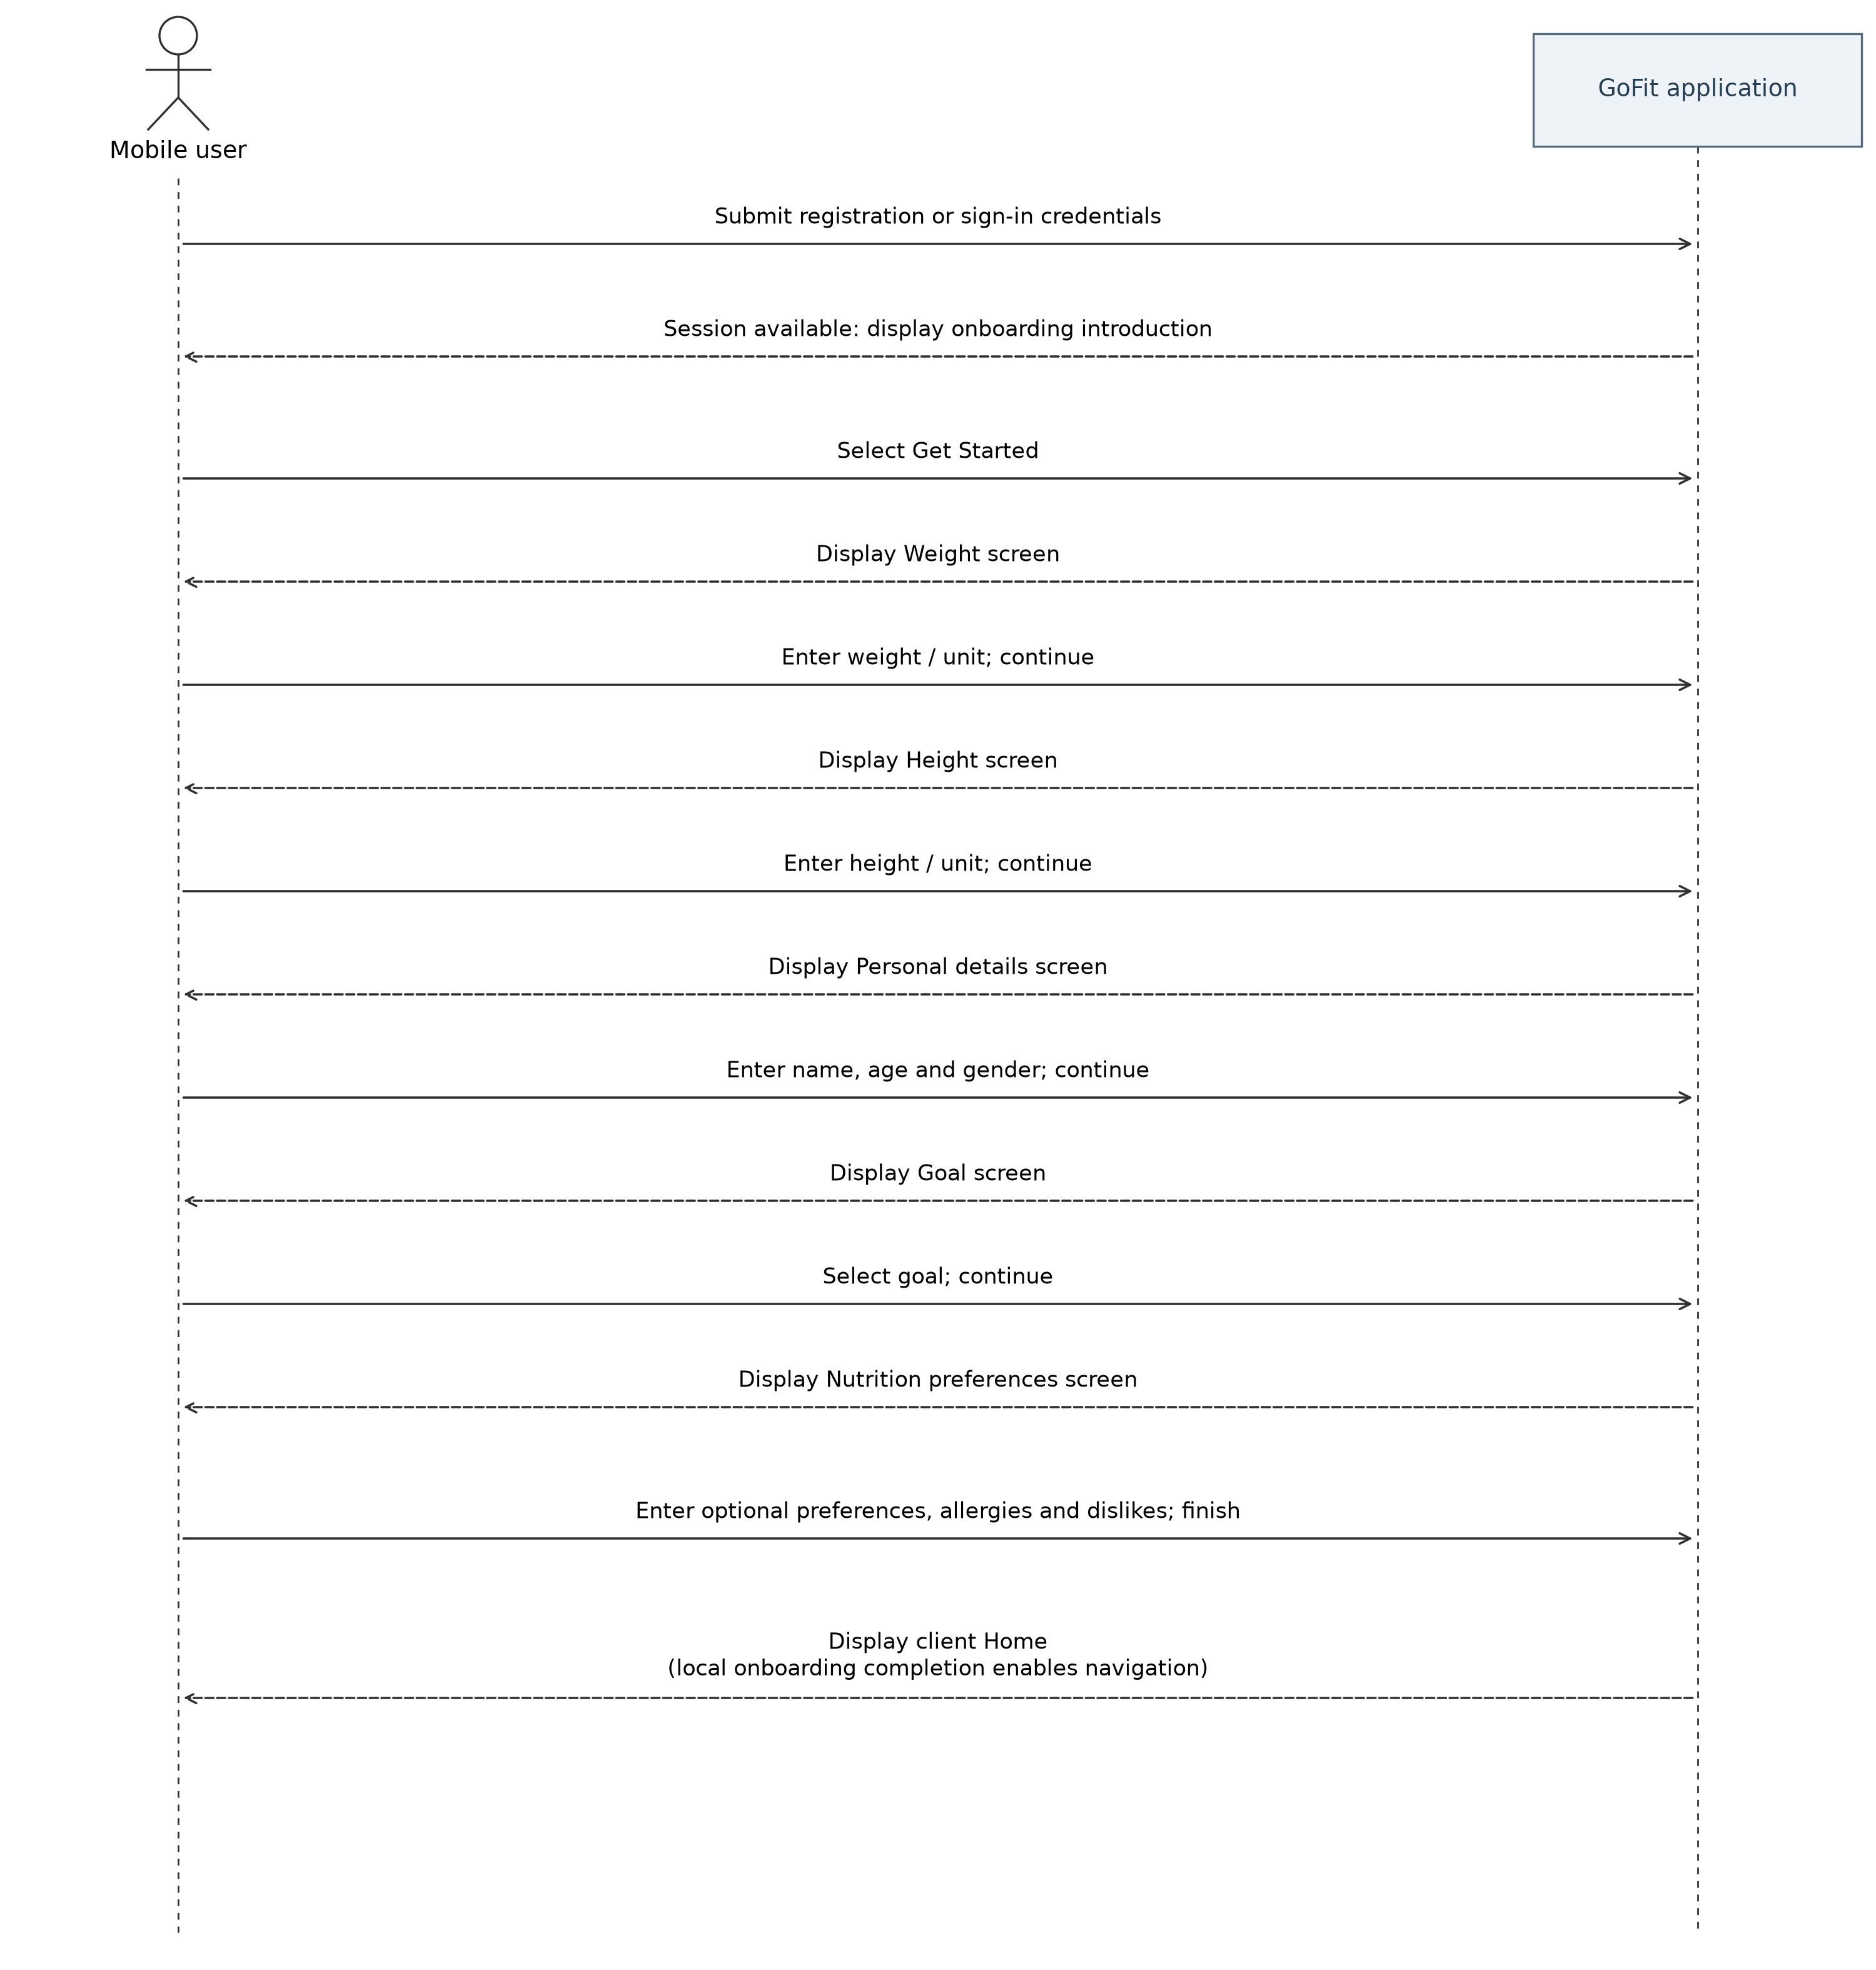
\includegraphics[width=0.92\linewidth]{figures/seq_auth_ssd.png}
\caption{System sequence diagram: Client authentication and full onboarding journey, with an authenticated session available}
\label{fig:seq_auth_ssd}
\end{figure}

\begin{figure}[H]
\centering
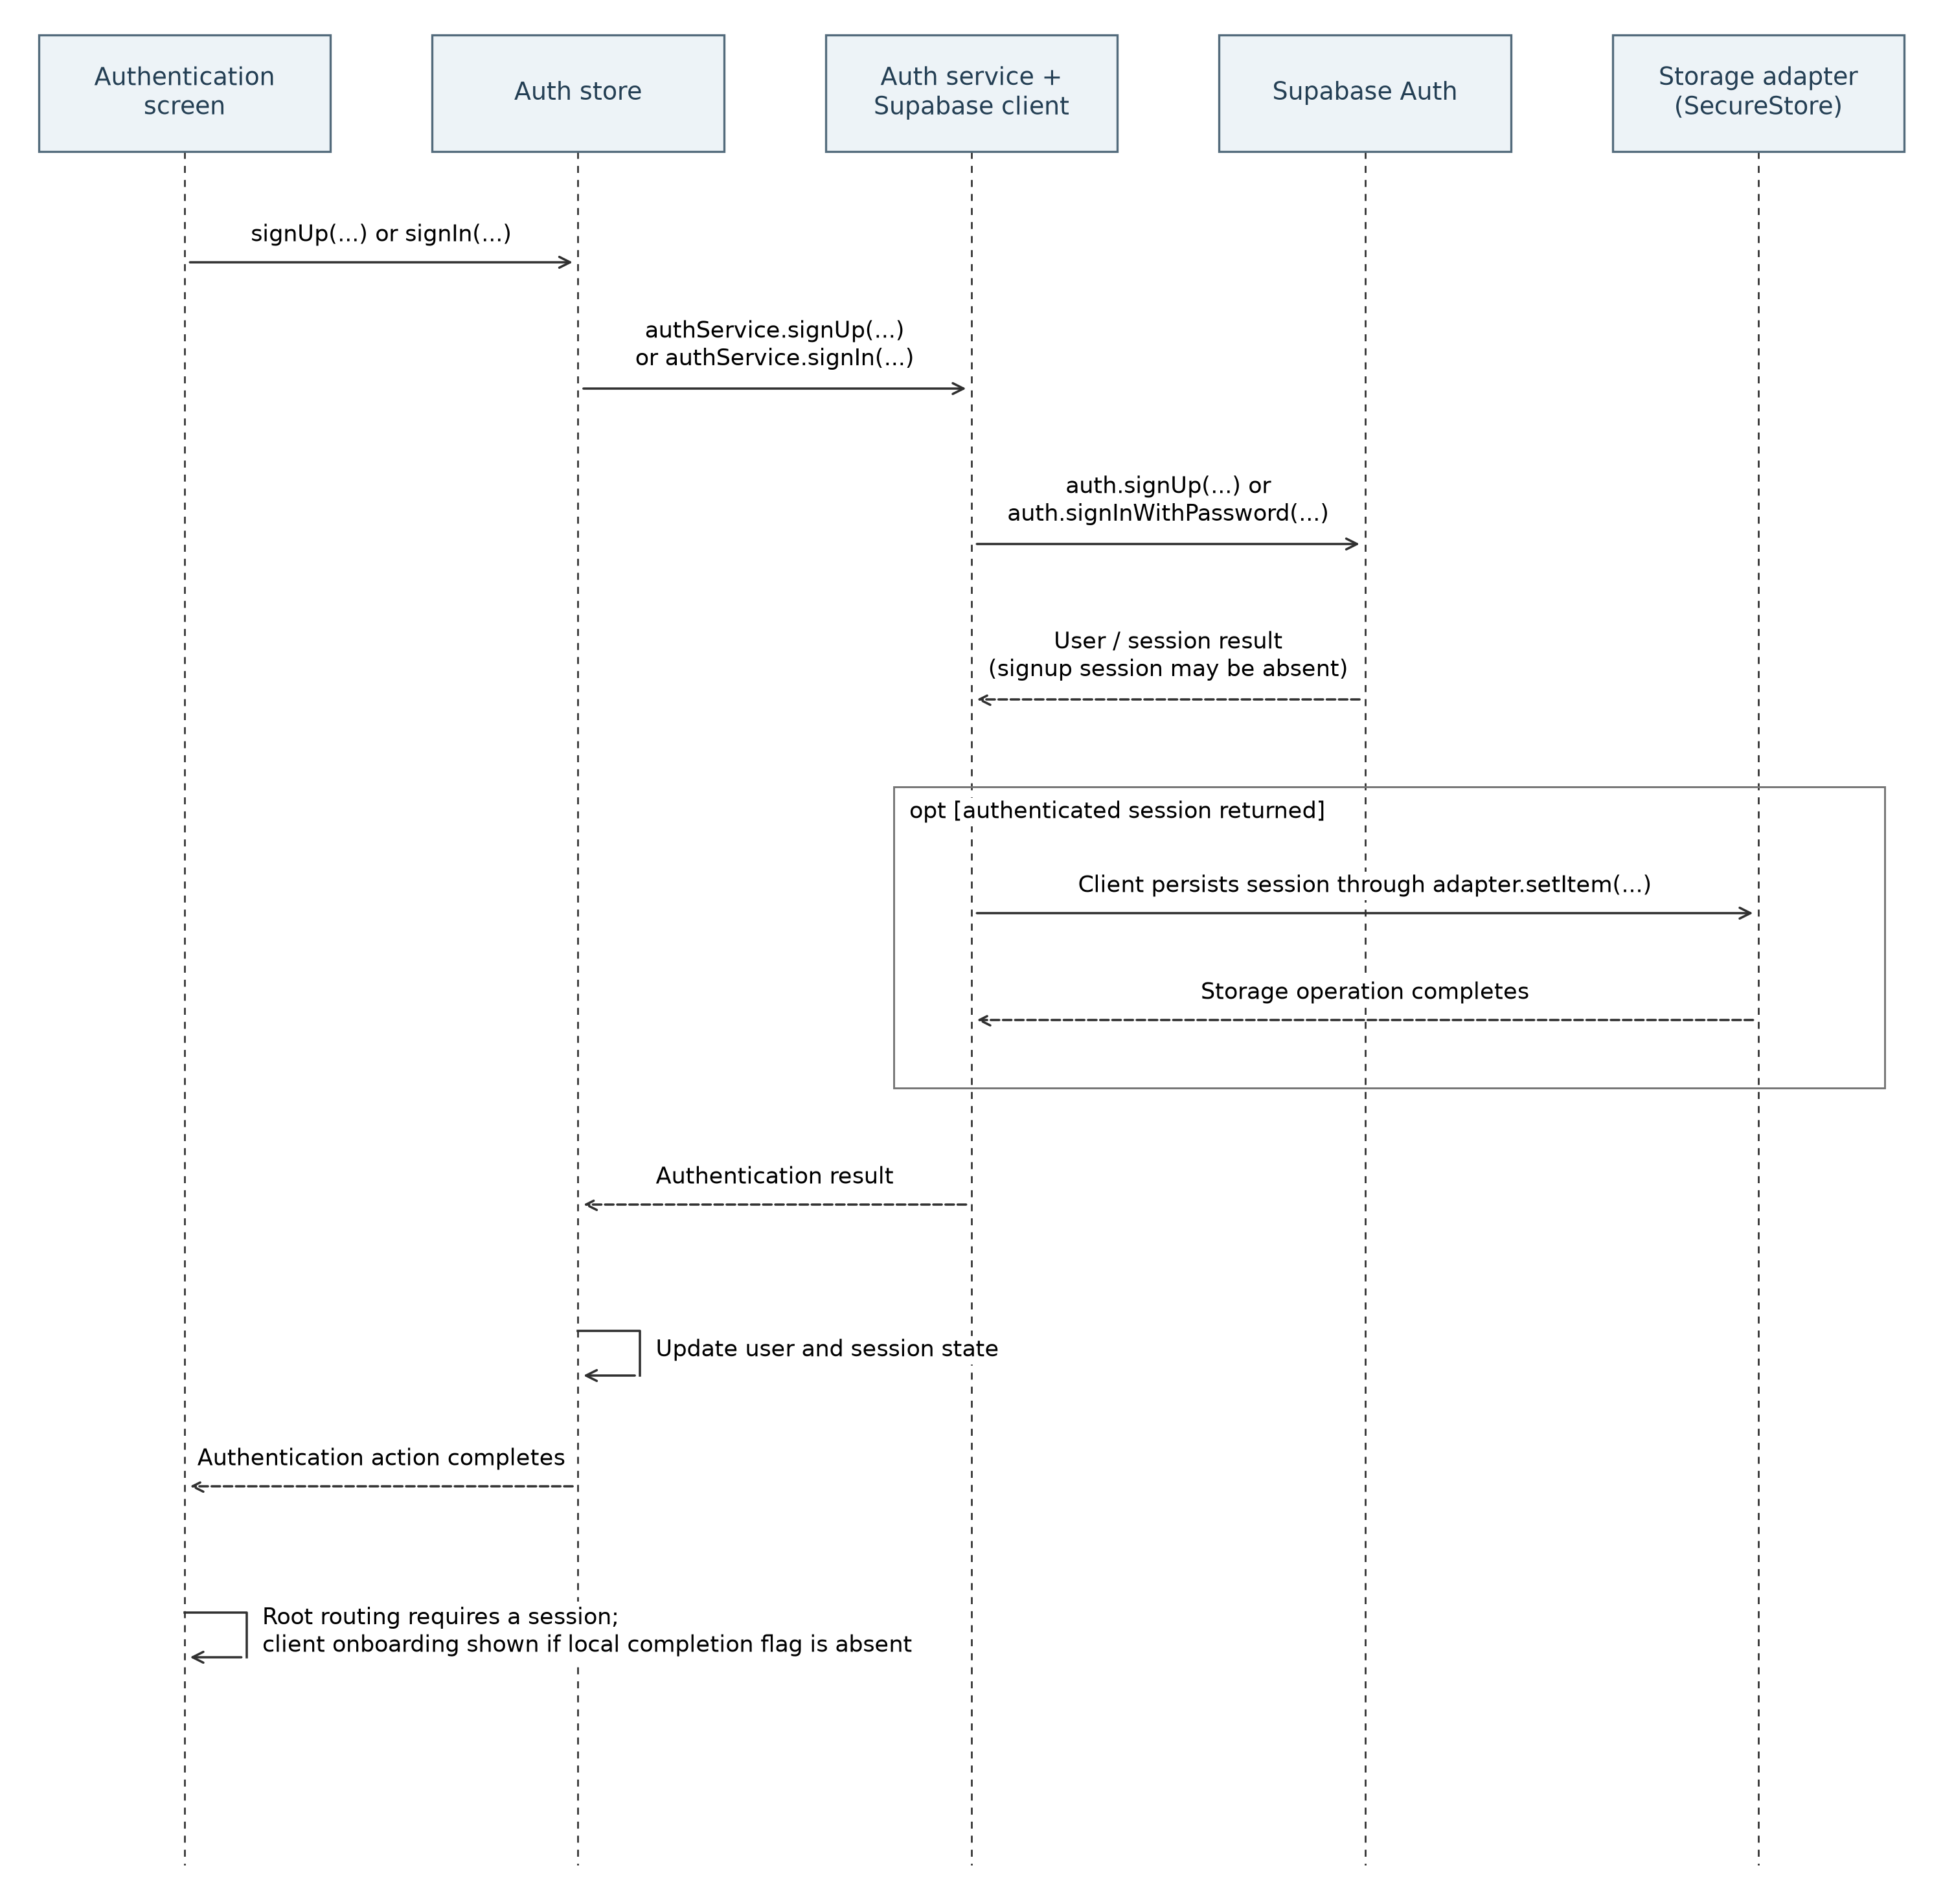
\includegraphics[width=0.92\linewidth]{figures/seq_auth_detailed.png}
\caption{Technical sequence diagram: Authentication and mobile session persistence}
\label{fig:seq_auth_detailed}
\end{figure}

Figure~\ref{fig:seq_auth_ssd} shows the full client onboarding journey through six registered screens: introduction, weight, height, personal details, goal, and nutrition preferences. Screen names in the responses make the navigation path explicit while retaining the application as a single system participant. This selected path assumes authentication yields a session and the user chooses the full form rather than Skip. Signup and sign-in are distinct operations: the signup screen schedules navigation to Login, while the root navigator also reacts to session availability. The diagram therefore does not imply that every registration configuration immediately permits onboarding. Existing locally completed client accounts bypass this form; coach onboarding is separate.

Figure~\ref{fig:seq_auth_detailed} selects the authentication and session-persistence interactions. The authentication screen calls the auth store, which delegates to the authentication service and configured Supabase client. The figure groups that service and client into one participant, but identifies the client as the owner of session persistence. When a session is returned, the client uses its configured storage adapter, backed by the application's SecureStore utility on Android and iOS. The client manages the storage keys and persisted session data. The utility supports chunking larger stored values and uses AsyncStorage as its web fallback. The client enables session persistence and automatic token refresh in its configured mobile path; these settings do not by themselves establish device-specific hardware security guarantees or successful persistence under all failures. Rate limiting, auth-state subscriptions, and activity tracking are outside this selected sequence.

\begin{figure}[H]
\centering
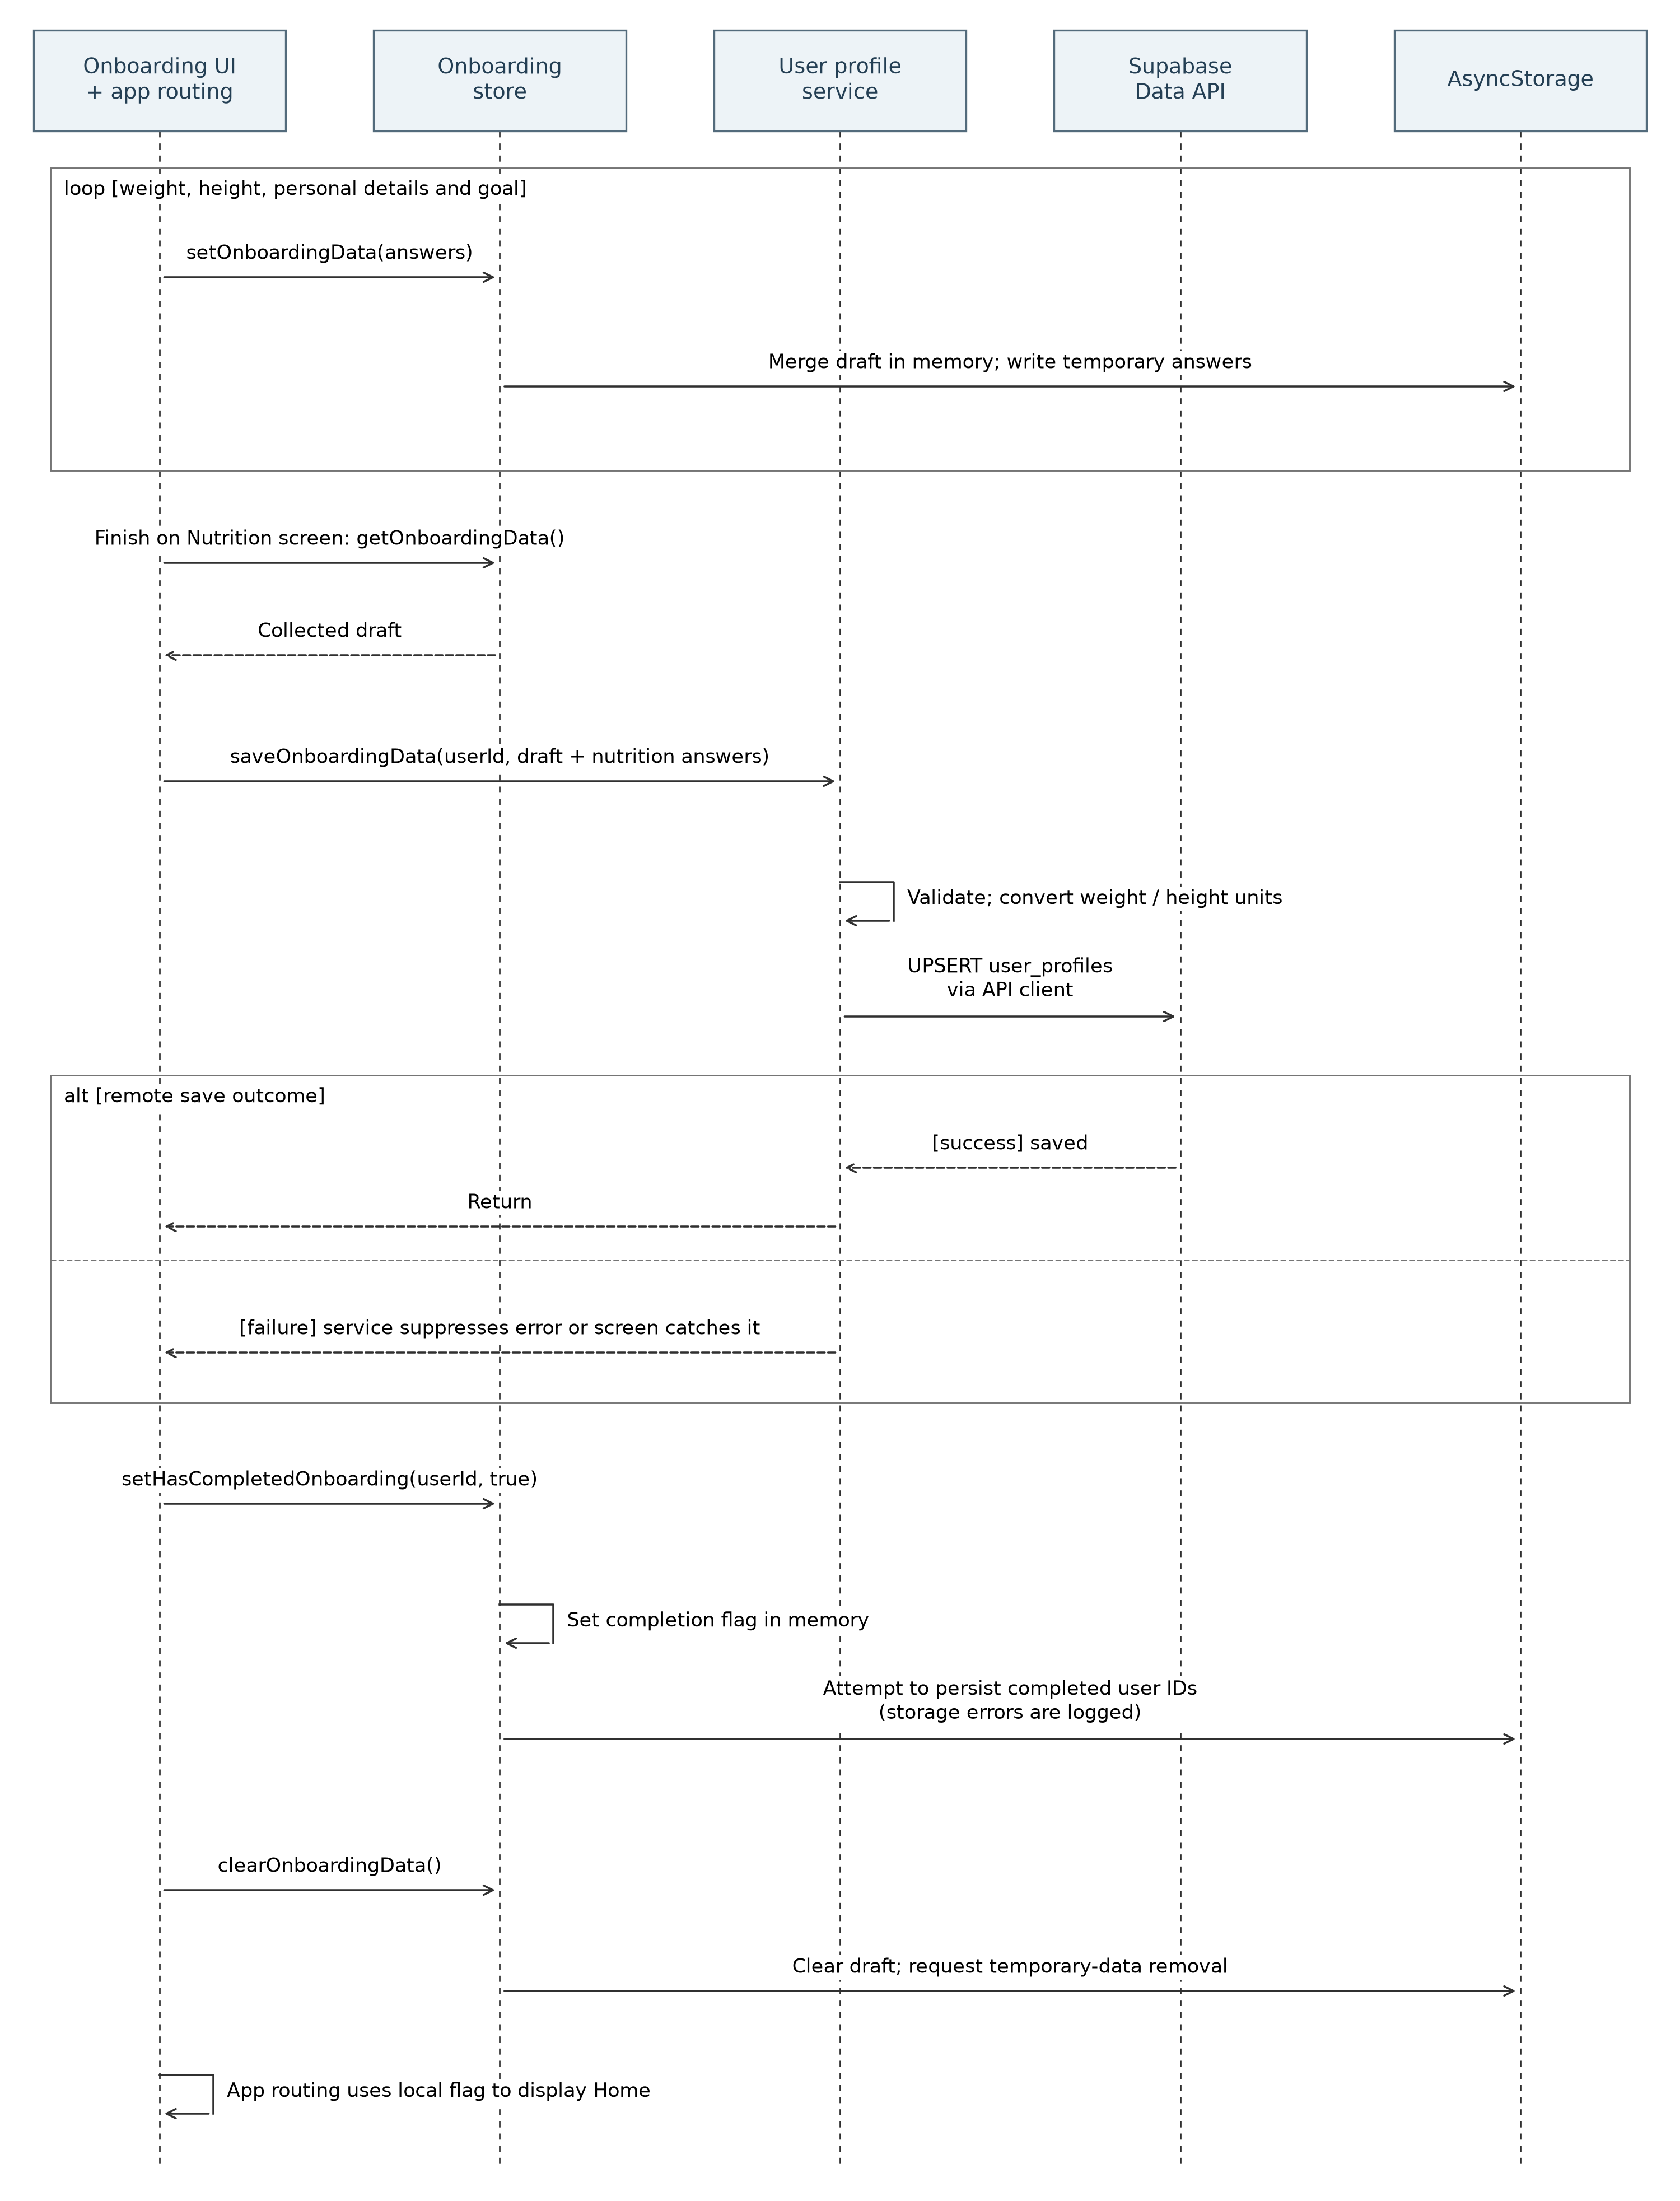
\includegraphics[width=0.95\linewidth]{figures/seq_auth_onboarding.png}
\caption{Technical sequence diagram: Client onboarding answers, profile-save outcomes, and local completion}
\label{fig:seq_auth_onboarding}
\end{figure}

Figure~\ref{fig:seq_auth_onboarding} separates profile persistence from local onboarding completion. The onboarding store merges intermediate answers and requests temporary persistence in AsyncStorage. On the Nutrition screen, the application combines those answers with nutrition preferences and calls the profile service. That service validates and converts weight and height before requesting an upsert into \texttt{user\_profiles} through the API client and Supabase Data API. Personal display-name metadata is updated separately after the profile-service call returns when a name was supplied; this optional operation is omitted from the figure. The profile service suppresses some errors, and the screen catches errors propagated from the profile or metadata operations. In either case, the screen can continue to mark onboarding complete locally. The store updates the in-memory completion flag before attempting its AsyncStorage write, logging storage failures rather than propagating them. Root routing depends on that local flag and the authenticated session, rather than a database onboarding-completion field. Reaching Home therefore does not prove that profile persistence succeeded. The final screen clears the temporary draft after marking local completion; the figure groups onboarding UI and root routing within one application participant.


\section{Realisation}

The mobile foundation was constructed with Expo SDK 54 and React Native running on the Hermes JavaScript engine. Modular navigation isolates auth, onboarding, and authenticated client tabs.


Authentication relies on Supabase Auth (GoTrue), with session JWTs and refresh tokens stored securely in expo-secure-store. Reactive session state is managed via Zustand authStore.


Workout execution decouples static workout templates from dynamic session logs. Sessions track precise start/end timestamps, calories burned, completed sets, and exercise order.


The rest timer engine features circular SVG progress animations, dual audio chimes (expo-av), haptic feedback (expo-haptics), auto-advance upon set completion, and background continuation.


\subsection{Interface Captures and Evidence Scope}

The following interface captures come from the retained October 2026 development-build and local-administration QA. They illustrate visible states and selected follow-up corrections, rather than proving internship-period delivery or complete workflow validation. Cropped excerpts omit unrelated records or identity columns; the original captures and their links to the QA records are retained in the accompanying evidence package. The report distinguishes configured, empty, cancelled, failed and successful states in the relevant captions.

The screenshot walkthrough covers client settings (Figure~\ref{fig:ui-client-settings}), workout creation (Figure~\ref{fig:ui-workout-selection-save}), nutrition (Figure~\ref{fig:ui-nutrition-extended}), coach follow-up (Figure~\ref{fig:ui-coach-followup-extended}) and the administration panel. The dedicated \textit{Administration Panel: Interface Walkthrough} begins on page~\pageref{sec:admin-panel-screens}; its user/coach management, catalog, dashboard and operational captures are separate from the mobile application. The List of Figures provides the individual image-group page numbers.

\subsection{Mobile Foundation and Navigation}

The first implementation challenge was to create a stable mobile foundation that could support both client and coach experiences. The application was structured around authentication screens, onboarding screens, protected app navigators, profile flows, and domain-specific feature stacks. This foundation is important because the rest of the product depends on role-aware routing: a visitor should not reach protected screens, an incomplete profile should be redirected to onboarding, and coach-specific flows should remain separated from standard client flows.


Stores organize reusable authentication, profile, workout and timer state, while service modules separate selected data operations from screen code. Table~\ref{tab:pdf-41-19} maps these responsibilities to inspected file names; it is not a historical sprint-end inventory or proof of maintainability.

\begingroup
\footnotesize
\setlength{\tabcolsep}{3pt}
\renewcommand{\arraystretch}{1.20}
\setlength{\LTpre}{5pt}
\setlength{\LTpost}{10pt}
\begin{longtable}{|L{3.67cm}|L{5.29cm}|L{5.73cm}|}
\caption{Sprint 1 architectural component mapping matrix}\label{tab:pdf-41-19} \\
\hline
\rowcolor{entetetab}
Architectural Tier & Technical Responsibility & Inspected artifacts for this scope \\ \hline
\endfirsthead
\hline
\rowcolor{entetetab}
Architectural Tier & Technical Responsibility & Inspected artifacts for this scope \\ \hline
\endhead
Presentation \& Routing & Organizes authentication, onboarding and workout interaction. & AuthNavigator.tsx, OnboardingNavigator.tsx and WorkoutSessionScreen.tsx. \\ \hline
Client State Management & Organizes reusable application state. & authStore.ts, profileStore.ts, workoutsStore.ts, timerStore.ts and uiStore.ts. \\ \hline
Domain Services & Implements authentication, workout data operations and completion retry. & services/auth.ts, services/workouts.ts and services/offlineQueue.ts. \\ \hline
Persistence \& Security & Handles session credentials, offline queue buffering, and cloud database access. & expo-secure-store, AsyncStorage, Supabase GoTrue Auth, PostgreSQL tables (user\_profiles, workouts, workout\_exercises, workout\_sessions). \\ \hline
Hardware Integration & Connects selected timer, feedback and media paths to device APIs. & Expo haptic, audio and video integration code; background execution requires separate device evidence. \\ \hline
\end{longtable}
\endgroup

Figure~\ref{fig:ui-client-entry} illustrates the onboarding introduction, existing-account Home and workout catalog as captured. Reaching Home does not establish completion or remote persistence of the full onboarding form.

\begin{figure}[H]
\centering
\begin{minipage}[t]{.29\linewidth}
\centering
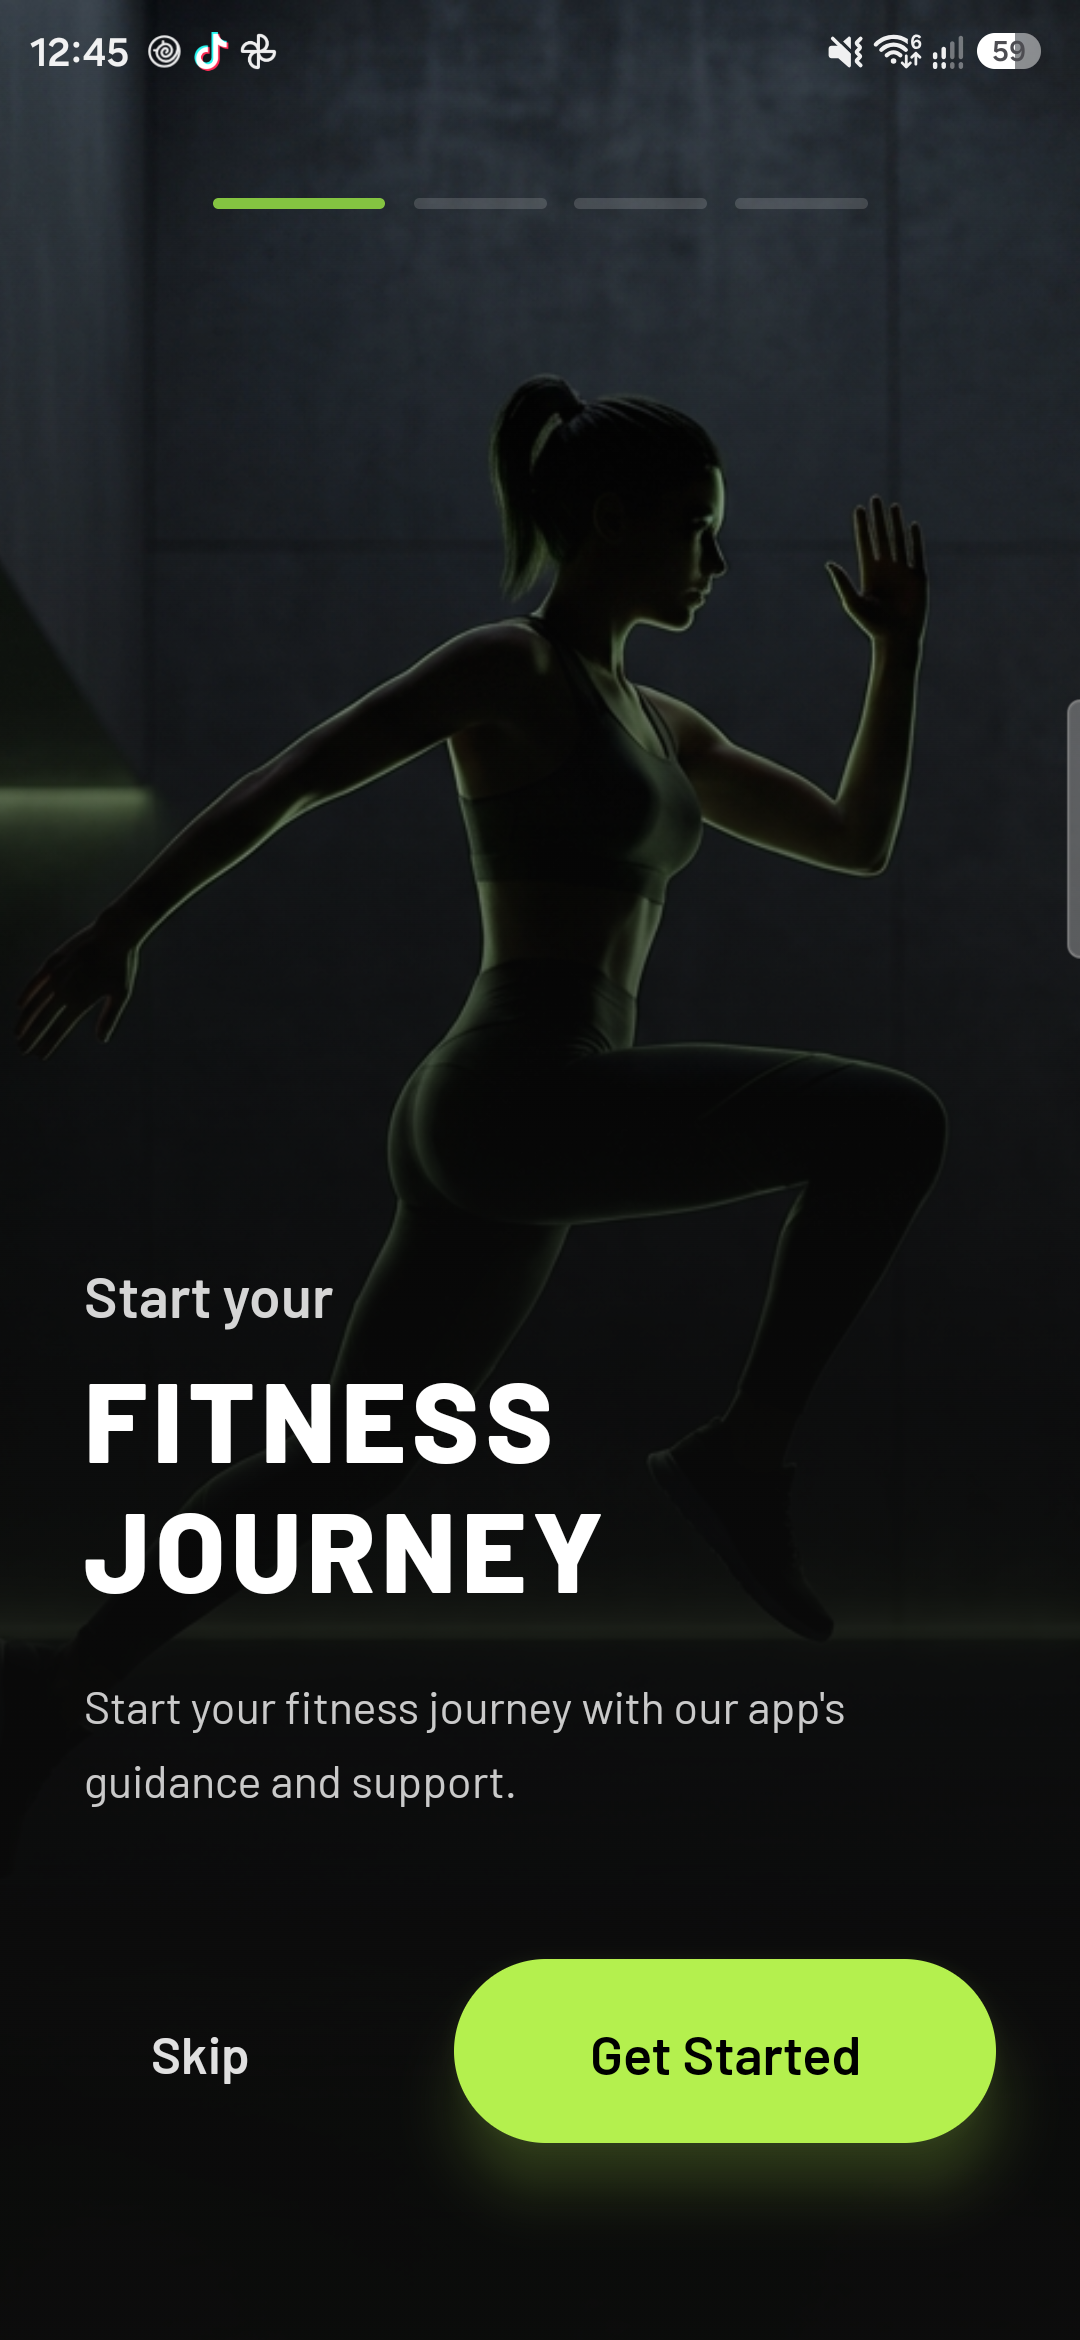
\includegraphics[width=\linewidth]{figures/screenshots/client-onboarding-introduction.png}
\par\smallskip{\footnotesize a) Onboarding introduction\par}
\end{minipage}
\hspace{0.025\linewidth}
\begin{minipage}[t]{.29\linewidth}
\centering
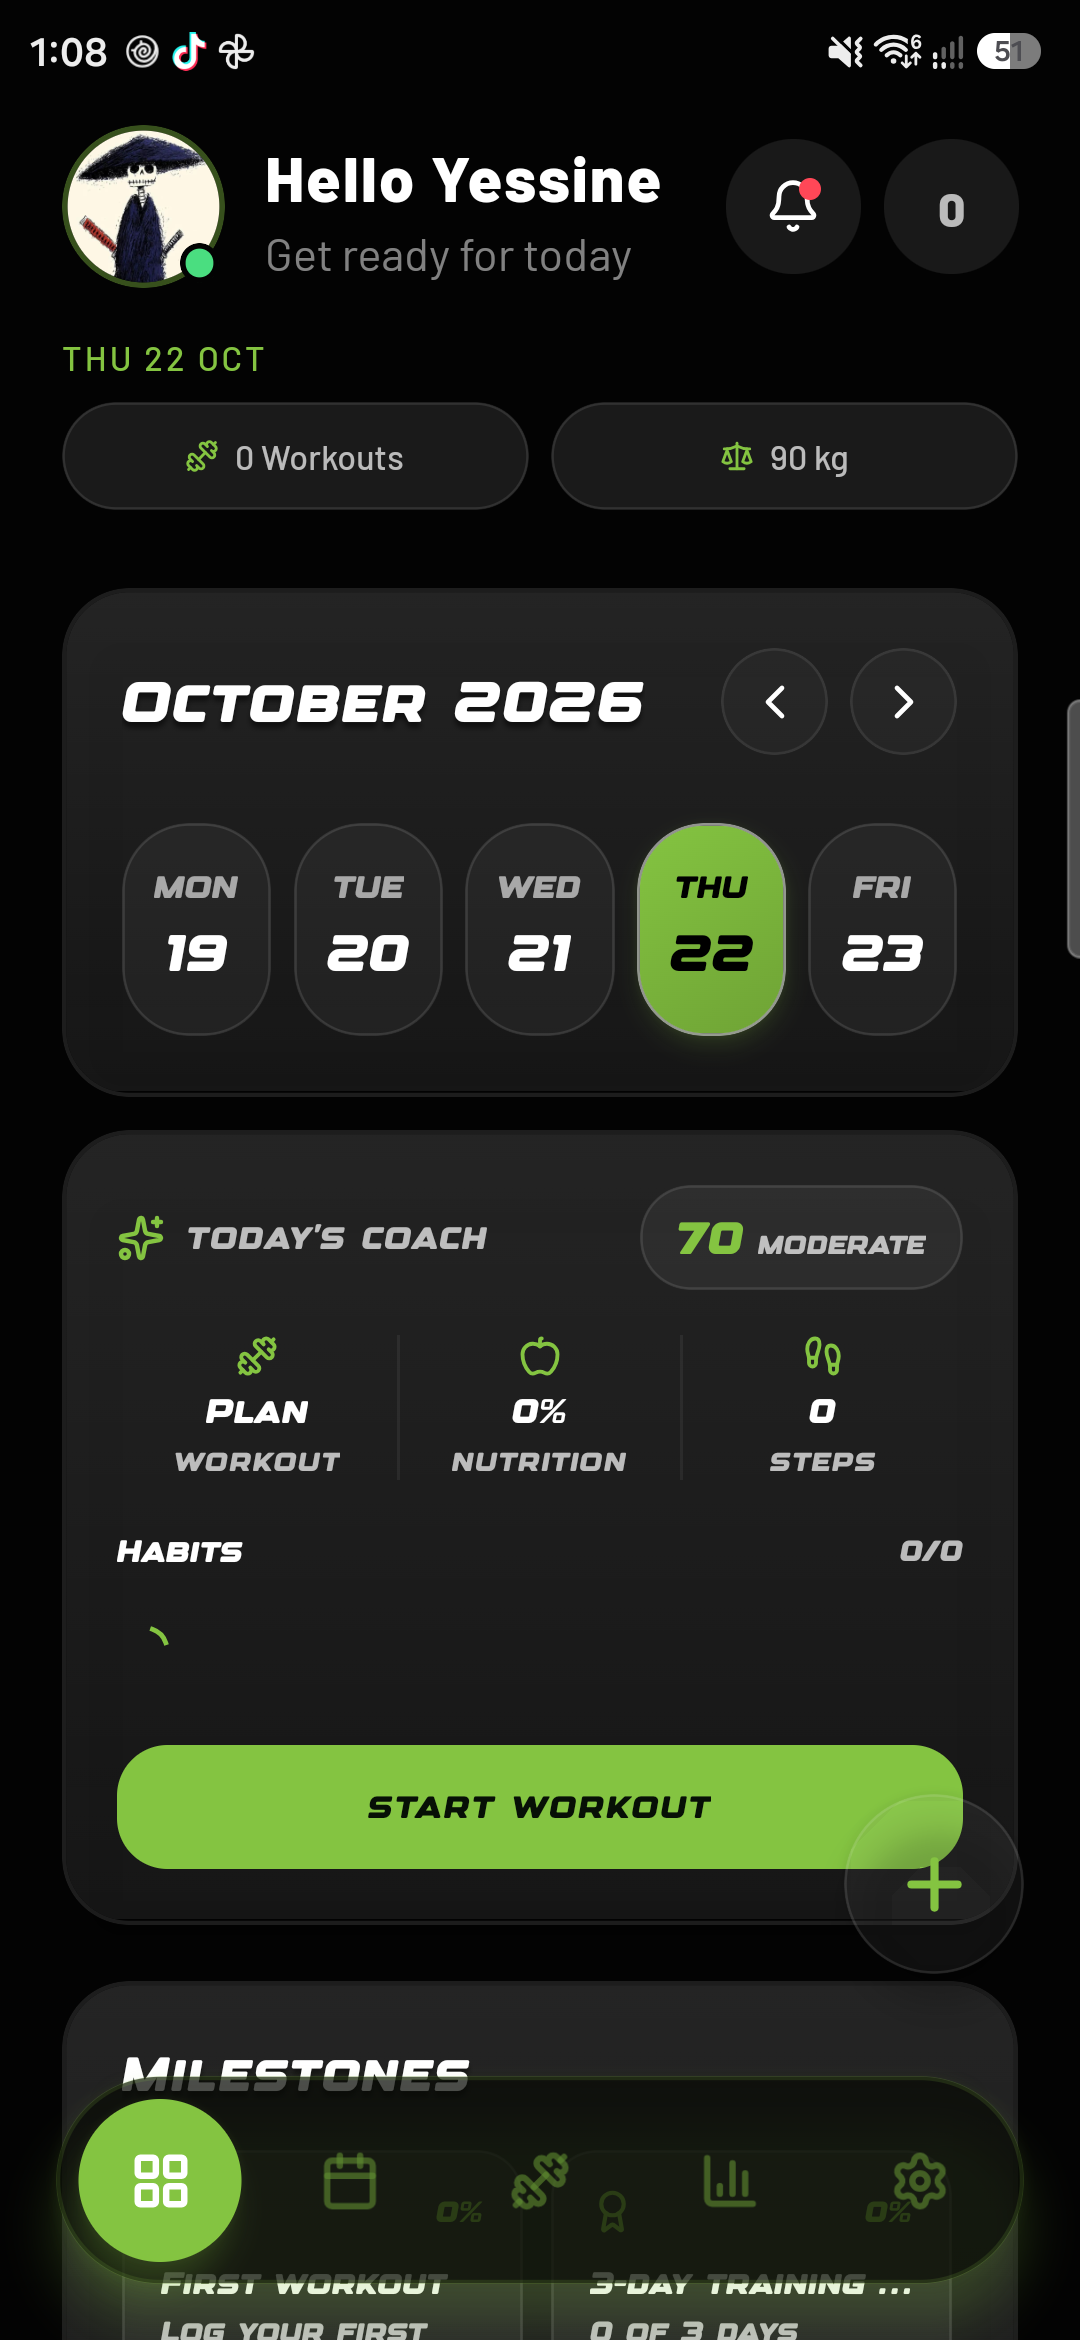
\includegraphics[width=\linewidth]{figures/screenshots/client-home-after-relaunch.png}
\par\smallskip{\footnotesize b) Home after session relaunch\par}
\end{minipage}
\hspace{0.025\linewidth}
\begin{minipage}[t]{.29\linewidth}
\centering
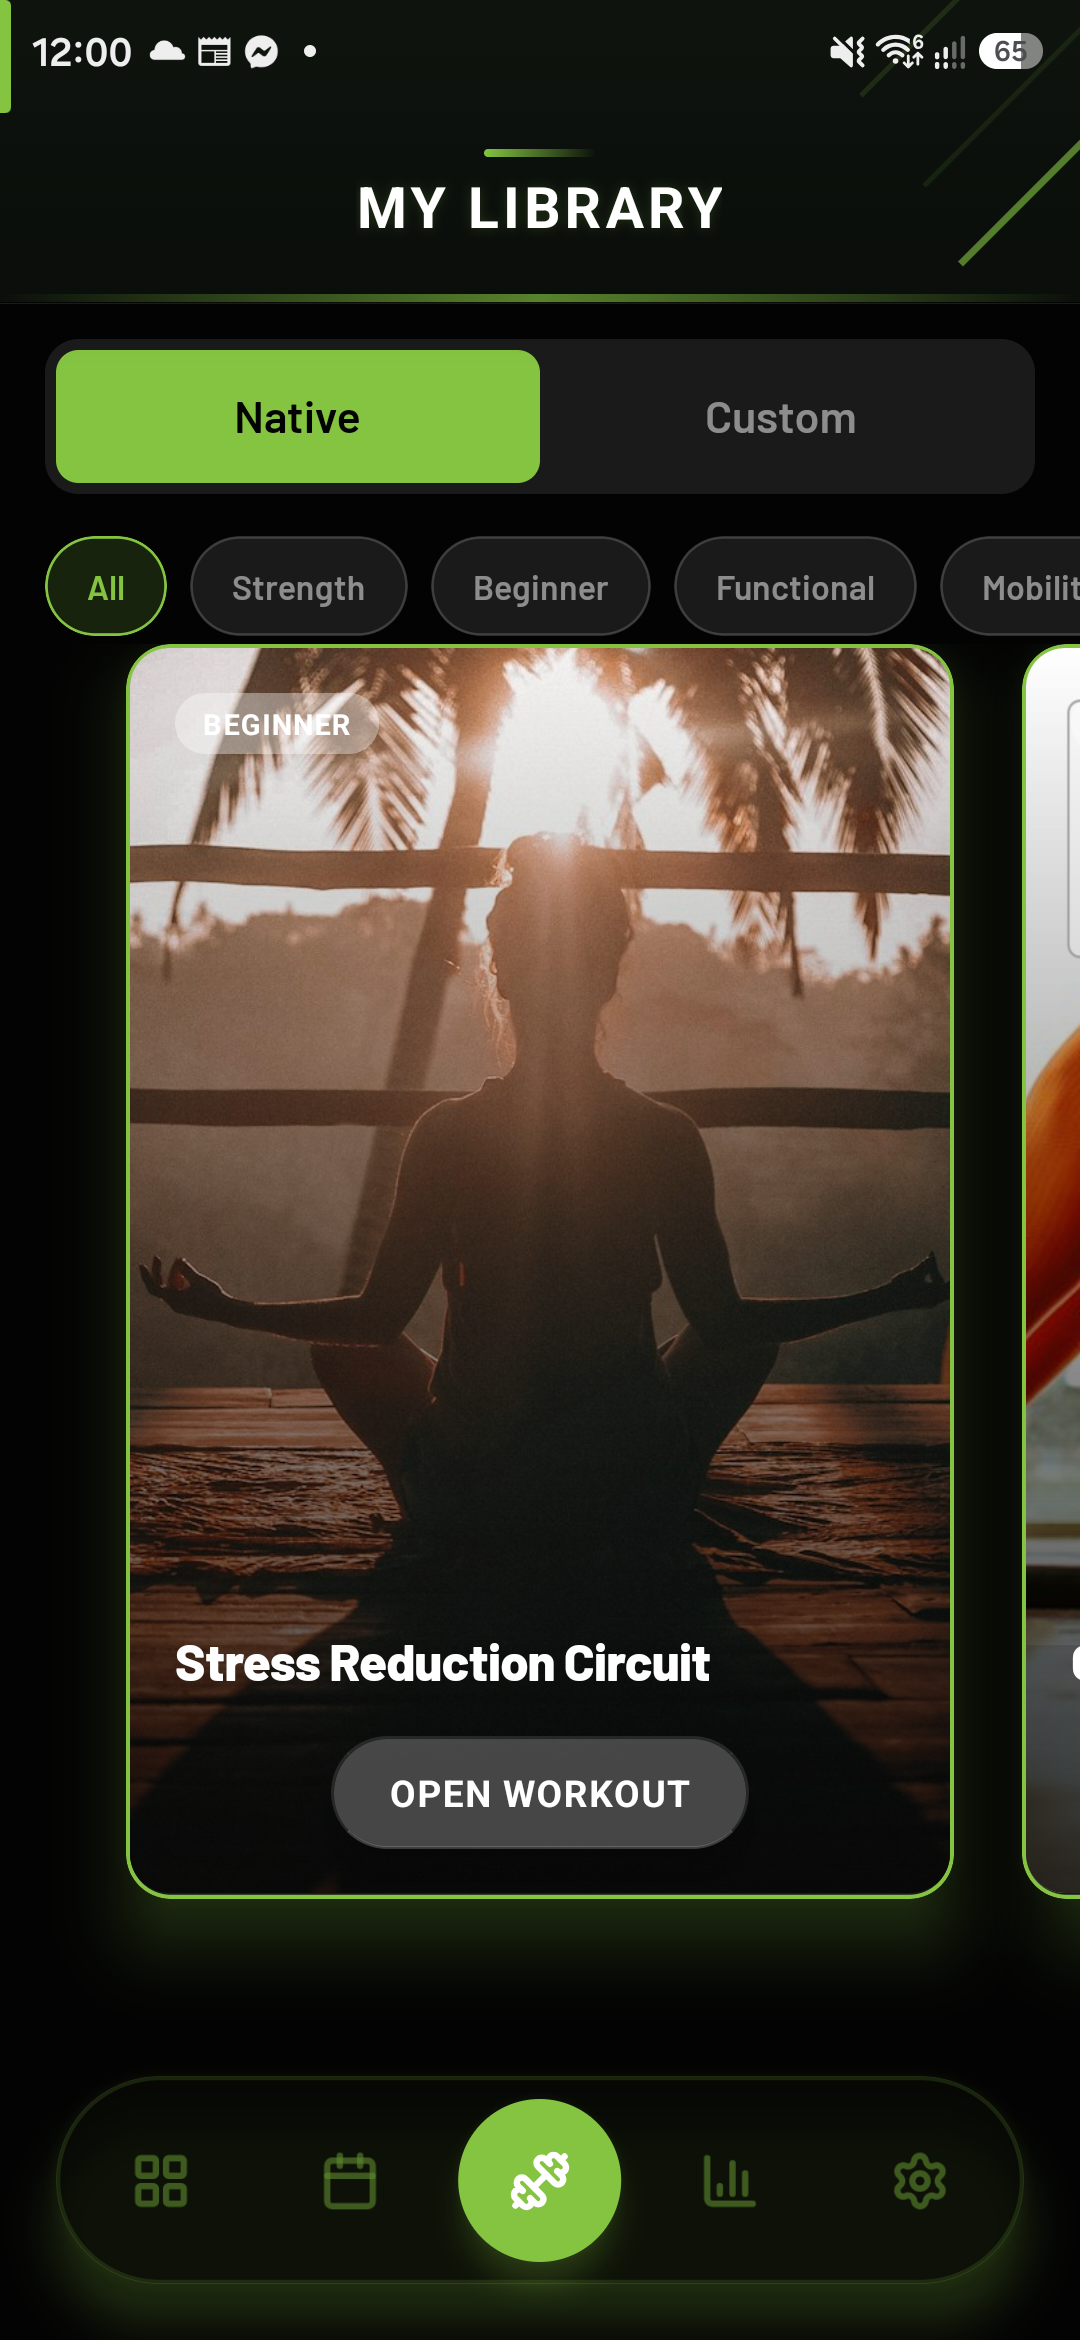
\includegraphics[width=\linewidth]{figures/screenshots/client-workout-catalog.png}
\par\smallskip{\footnotesize c) Native workout catalog\par}
\end{minipage}
\caption{Interface captures: onboarding introduction, existing-account Home and workout catalog (October development build).}
\label{fig:ui-client-entry}
\end{figure}

Figures~\ref{fig:ui-client-settings} and~\ref{fig:ui-client-reminder-settings} illustrate additional client controls. Their captured preferences do not independently establish every save, translation or notification-delivery outcome.

\begin{figure}[H]
\centering
\begin{minipage}[t]{.29\linewidth}
\centering
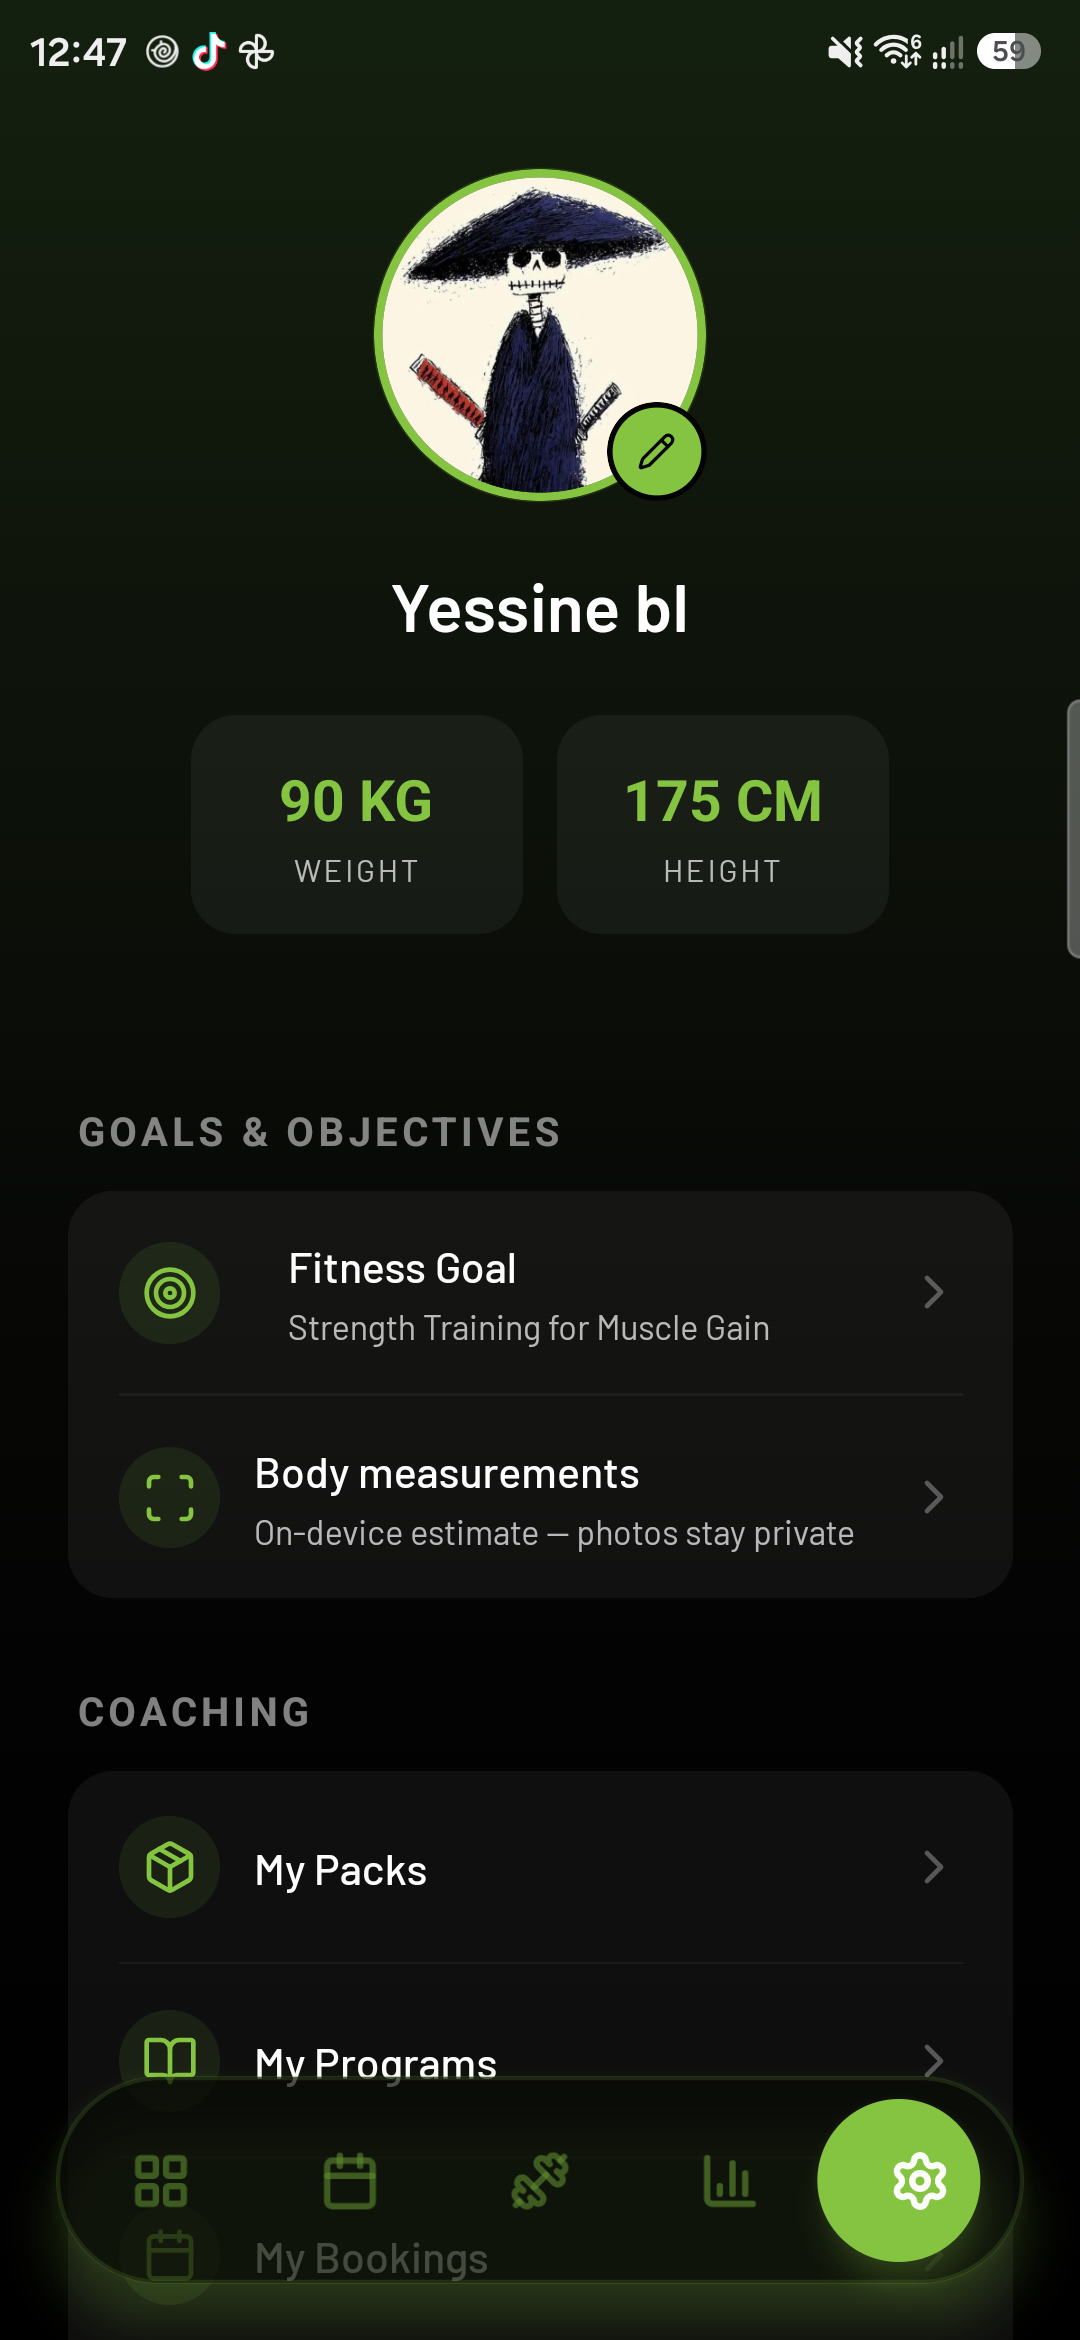
\includegraphics[width=\linewidth]{figures/screenshots/client-profile-overview.png}
\par\smallskip{\footnotesize a) Profile and feature entry points\par}
\end{minipage}
\hspace{0.025\linewidth}
\begin{minipage}[t]{.29\linewidth}
\centering
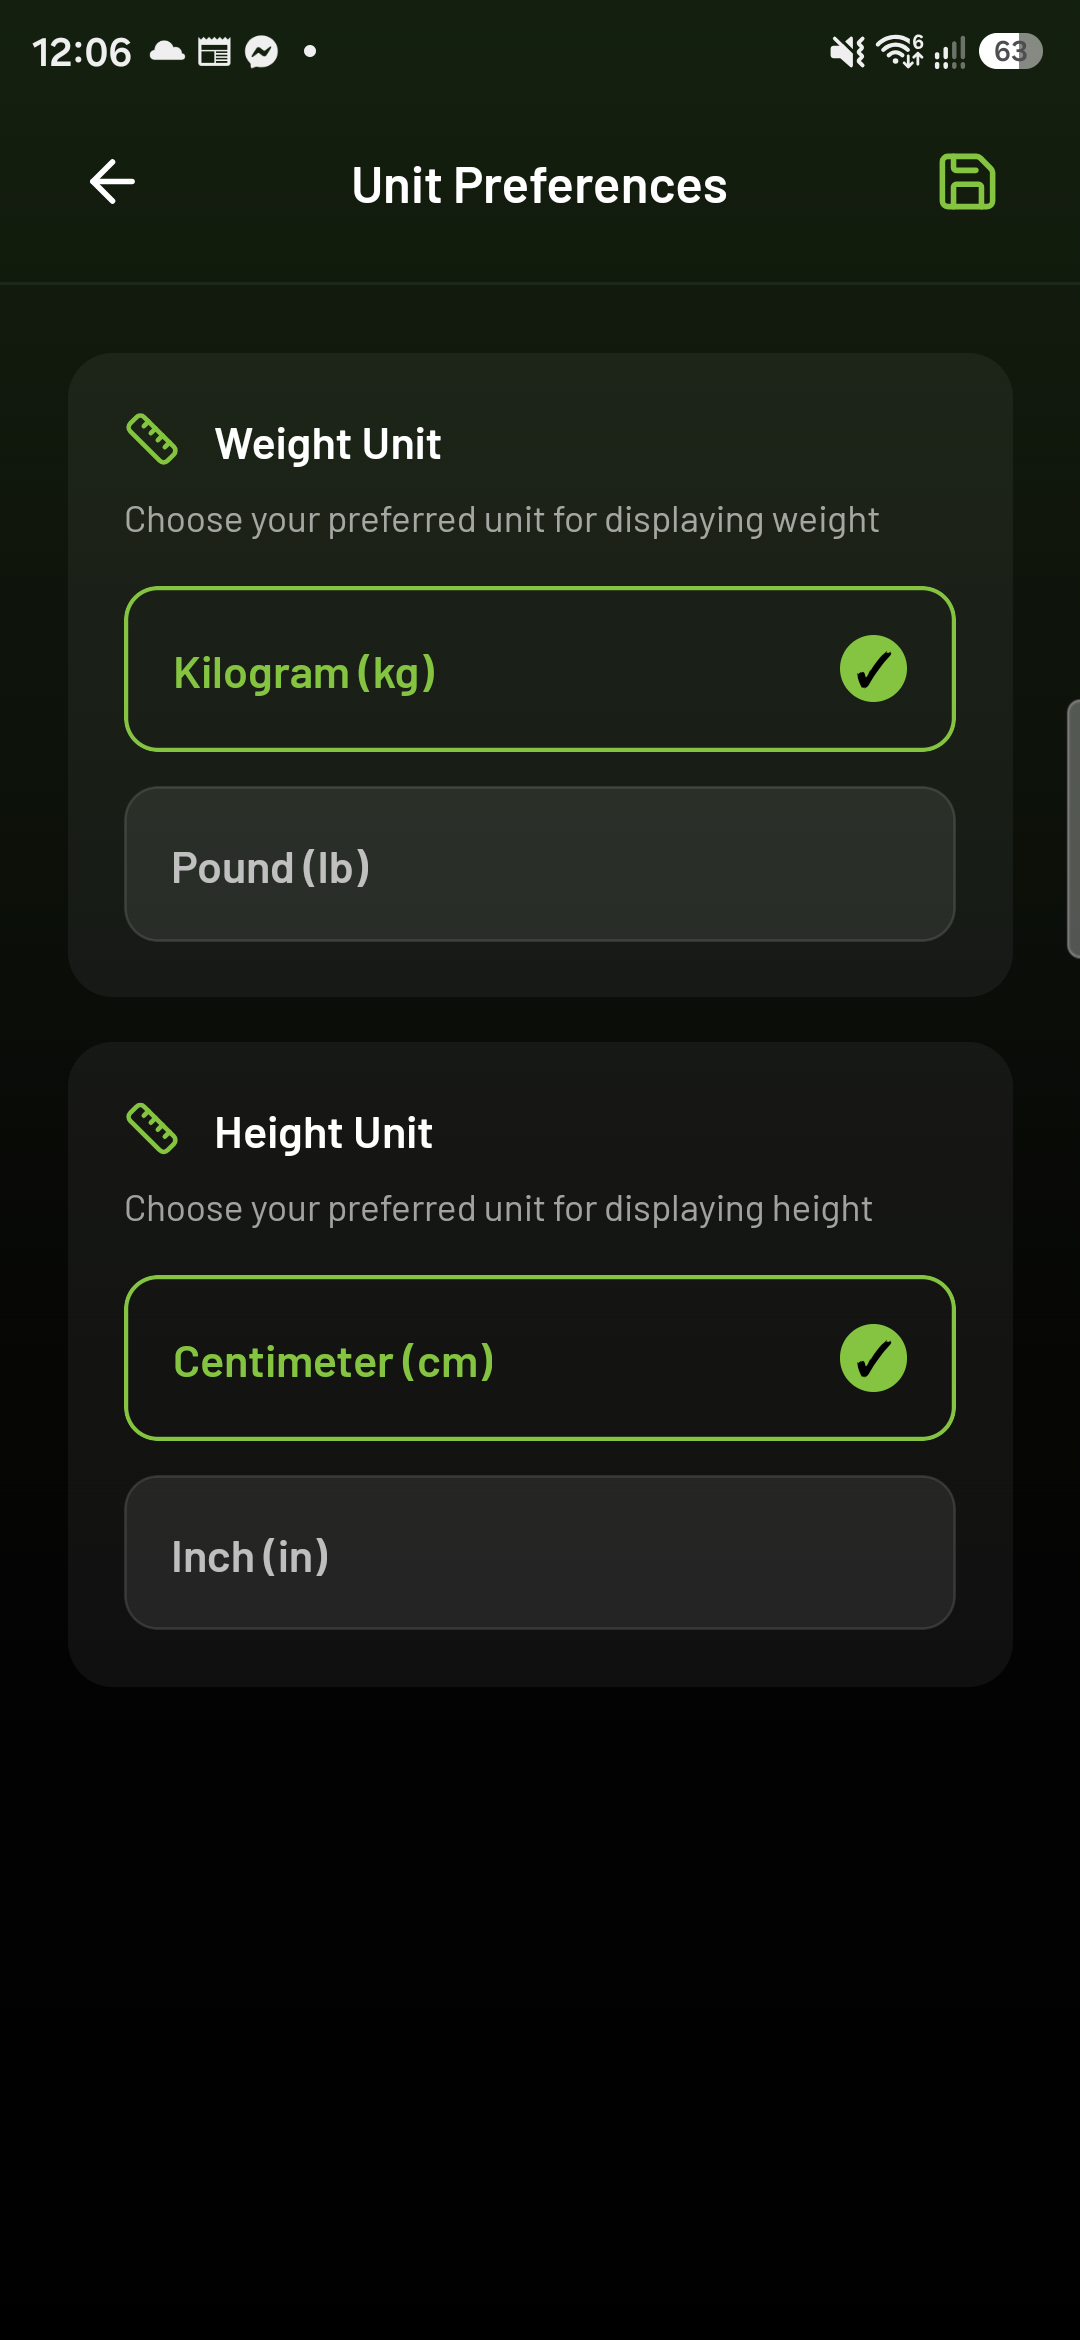
\includegraphics[width=\linewidth]{figures/screenshots/client-unit-preferences.png}
\par\smallskip{\footnotesize b) Weight and height units\par}
\end{minipage}
\hspace{0.025\linewidth}
\begin{minipage}[t]{.29\linewidth}
\centering

\includegraphics[width=\linewidth]{figures/screenshots/client-language-options.png}
\par\smallskip{\footnotesize c) Language selection\par}
\end{minipage}
\caption{Client interface walkthrough: profile overview, unit preferences and language selection.}
\label{fig:ui-client-settings}
\end{figure}

\begin{figure}[H]
\centering
\begin{minipage}[t]{.31\linewidth}
\centering
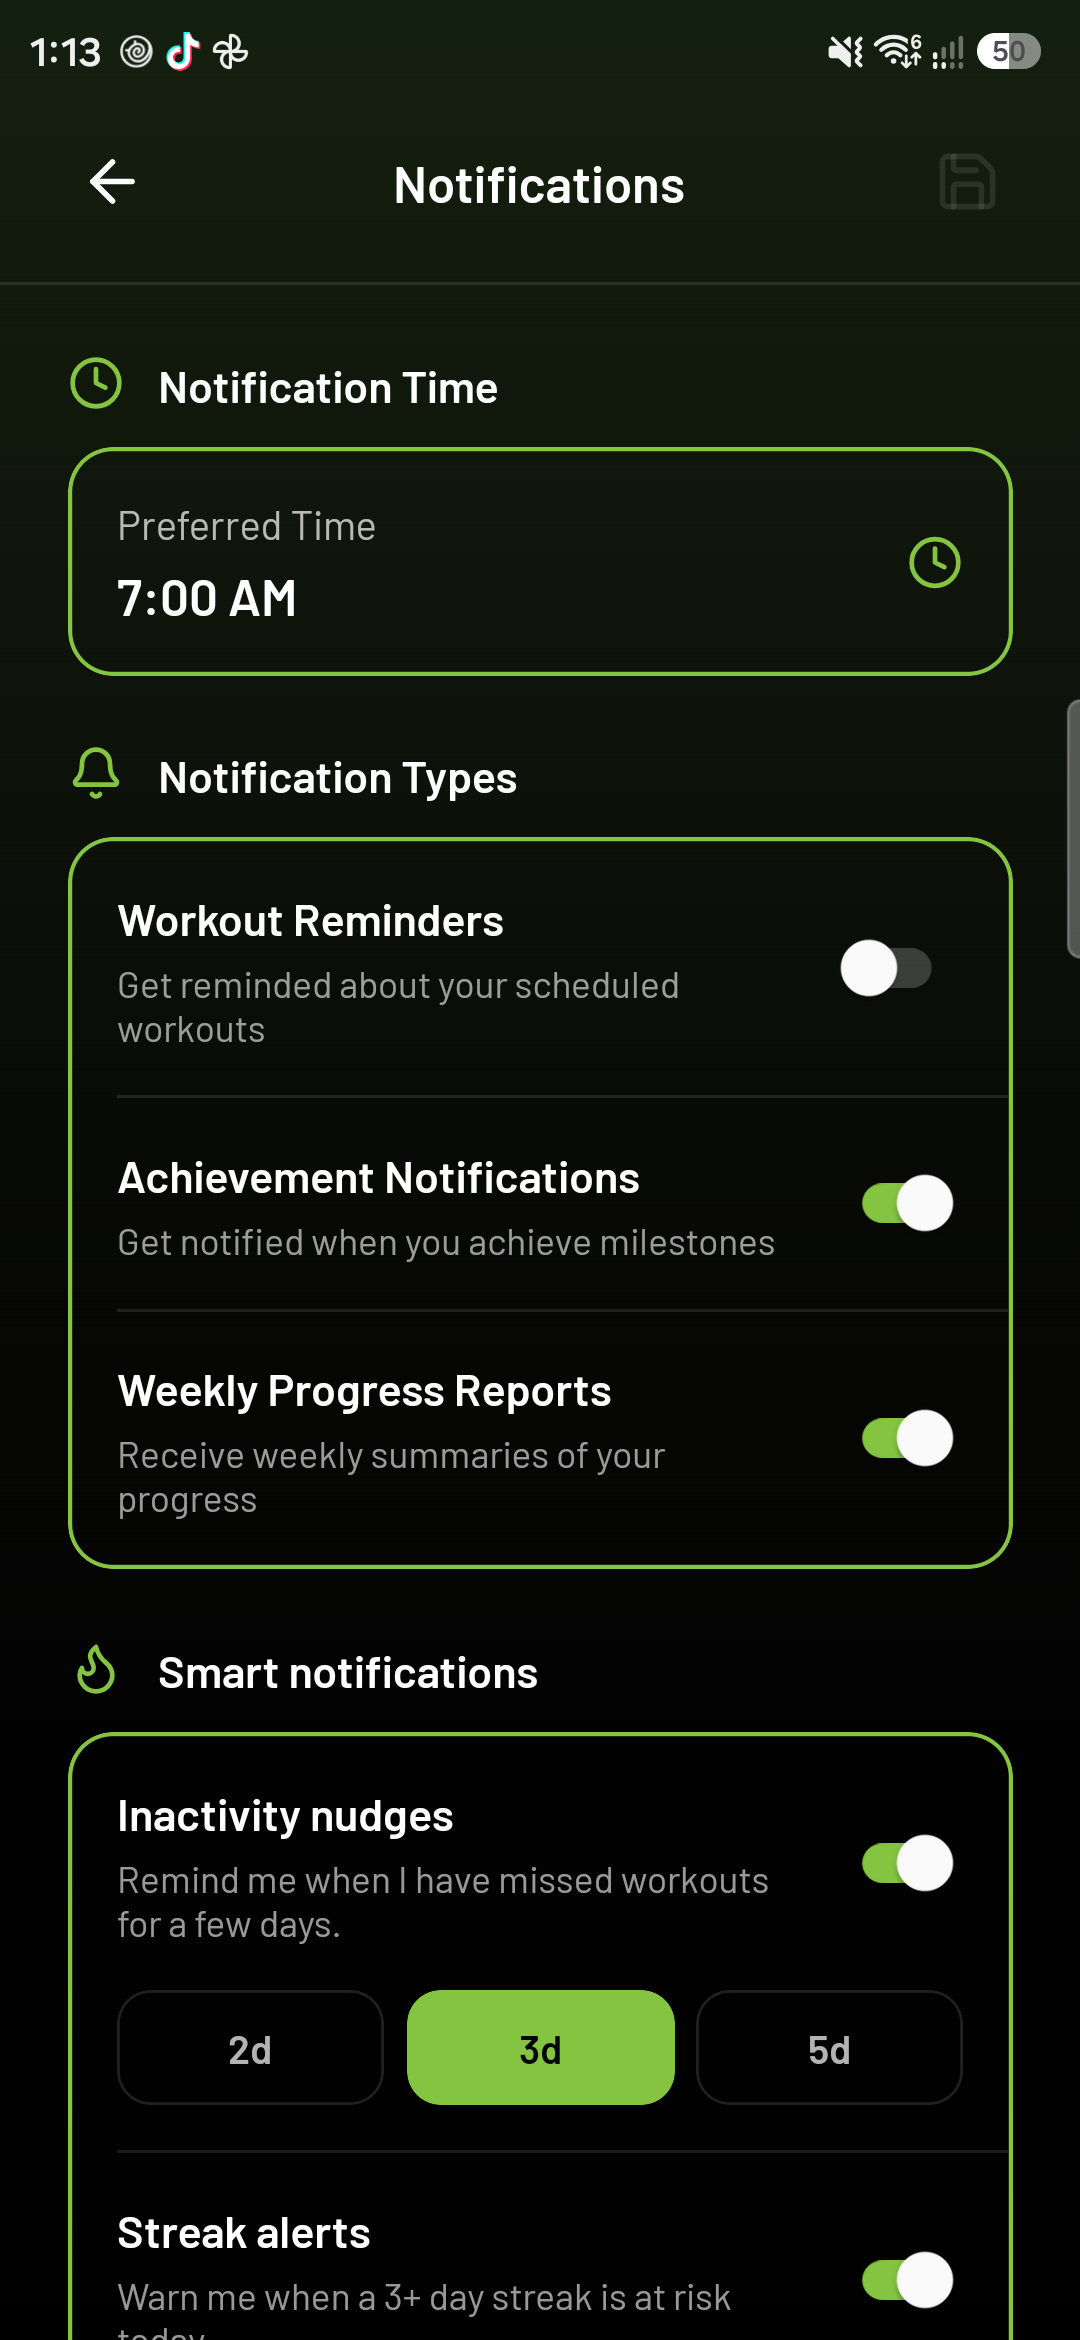
\includegraphics[width=\linewidth]{figures/screenshots/client-reminder-preferences.png}
\par\smallskip{\footnotesize a) Notification and reminder preferences\par}
\end{minipage}
\caption{Client interface walkthrough: reminder preferences as captured; scheduled delivery is assessed separately.}
\label{fig:ui-client-reminder-settings}
\end{figure}

\subsection{Workout Core and Rest Timer}

The workout core was implemented around the distinction between a workout template and an executed workout session. A workout template defines the exercises, order, difficulty, target muscle groups, and expected configuration. A workout session stores timestamps, duration, notes and exercise snapshots with configured sets/repetitions, entered weights and completion flags. Those snapshots do not independently measure performed repetitions or RPE. This separation is essential because the same workout can be performed many times while producing different session histories.


The rest timer was treated as a real workout tool rather than a decorative countdown. It includes start, pause, resume, warning cues, haptic feedback, audio cues, auto-advance options, and persisted preferences. This improves usability during training because users often interact with the timer under fatigue and need clear feedback without navigating away from the session.


Figure~\ref{fig:ui-workout-configuration} shows an exercise prescription and the workout-builder form. Set, repetition and rest fields describe the prescription; no active-session, timer-expiry or offline result is inferred from these images.

\begin{figure}[H]
\centering
\begin{minipage}[t]{.31\linewidth}
\centering
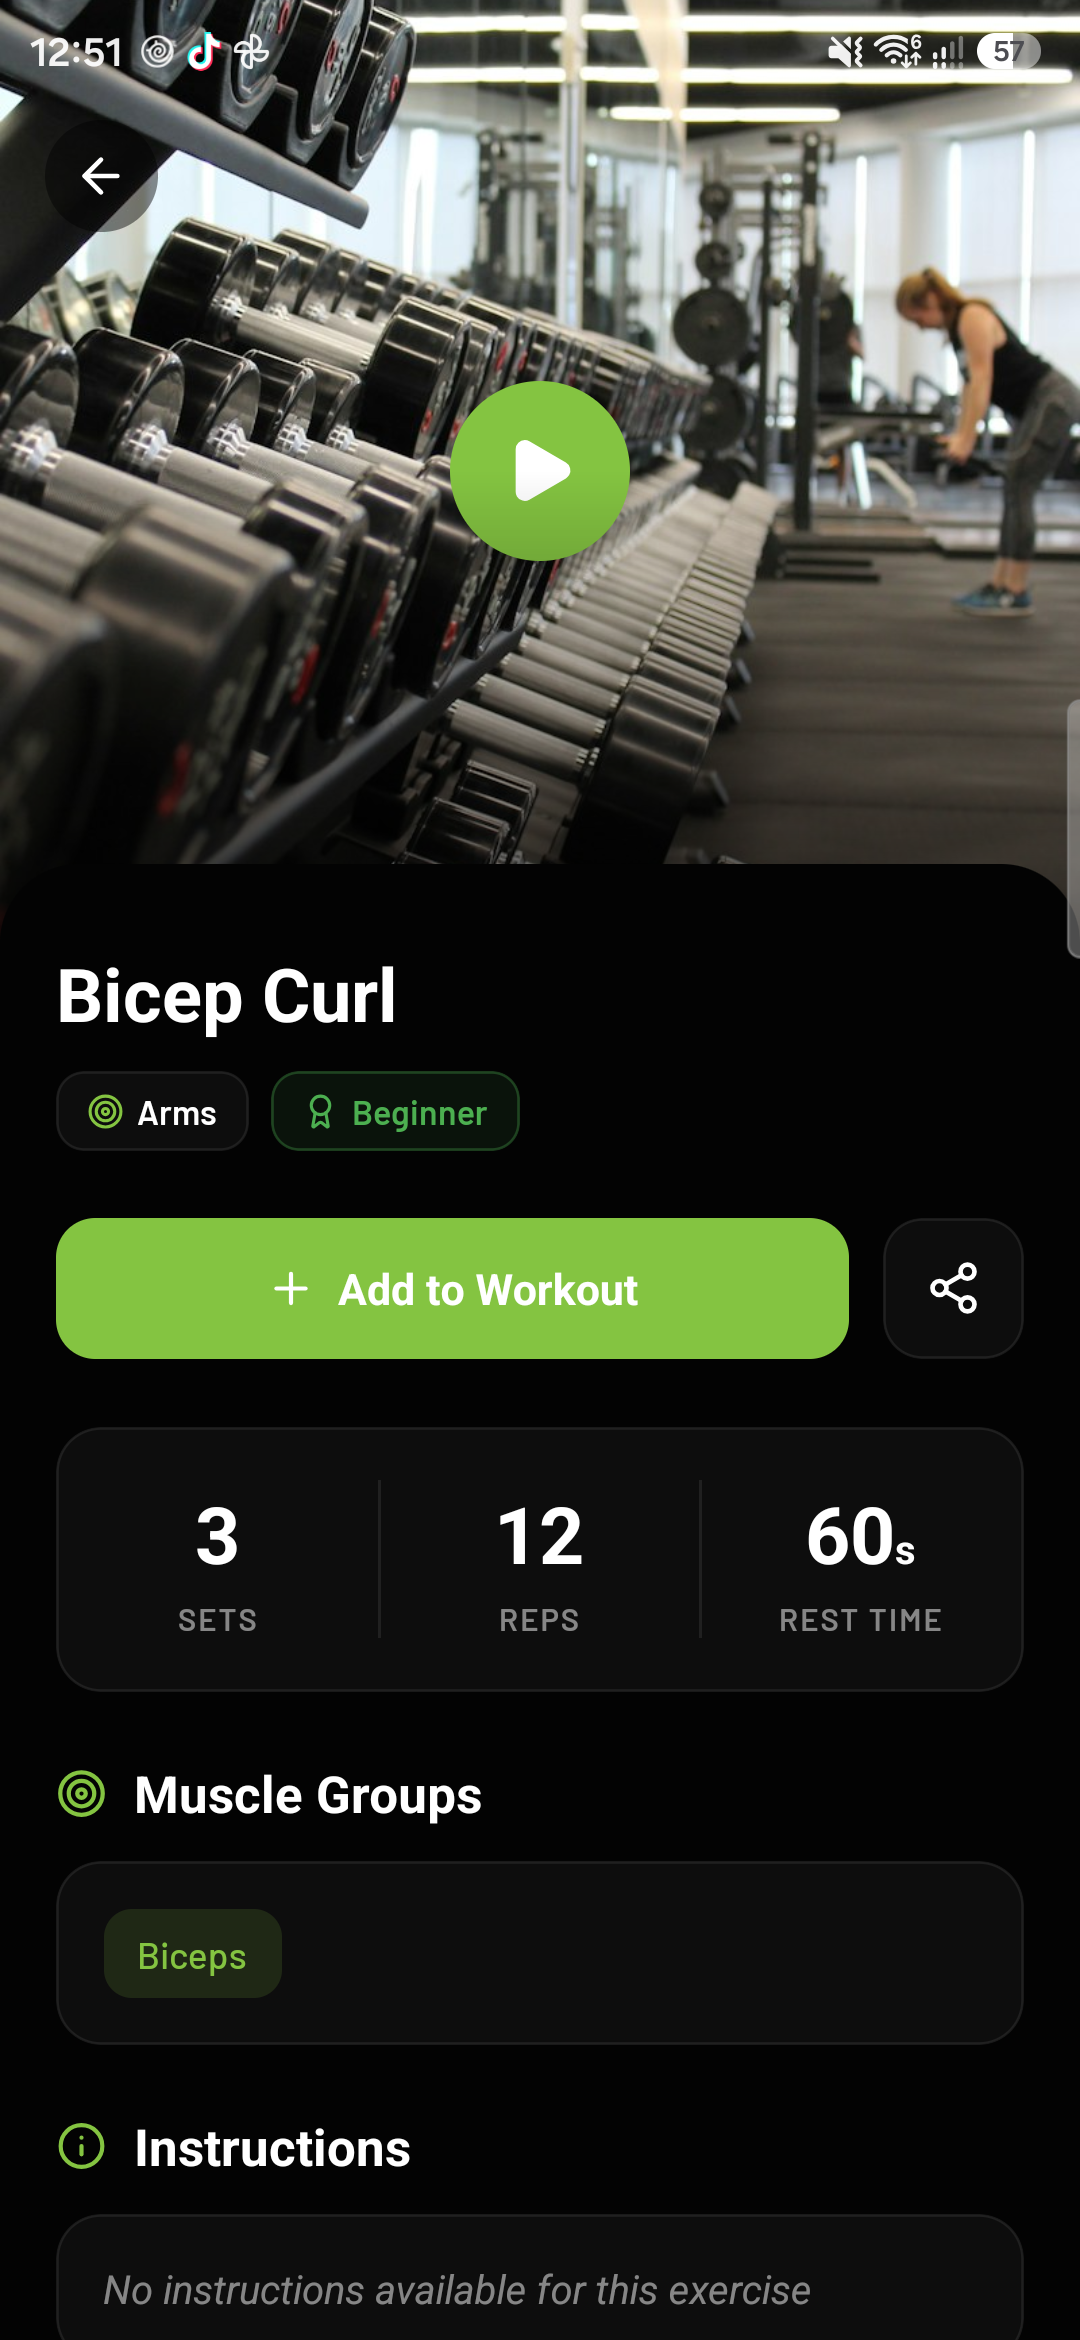
\includegraphics[width=\linewidth]{figures/screenshots/client-exercise-detail.png}
\par\smallskip{\footnotesize a) Exercise detail\par}
\end{minipage}
\hspace{0.025\linewidth}
\begin{minipage}[t]{.31\linewidth}
\centering
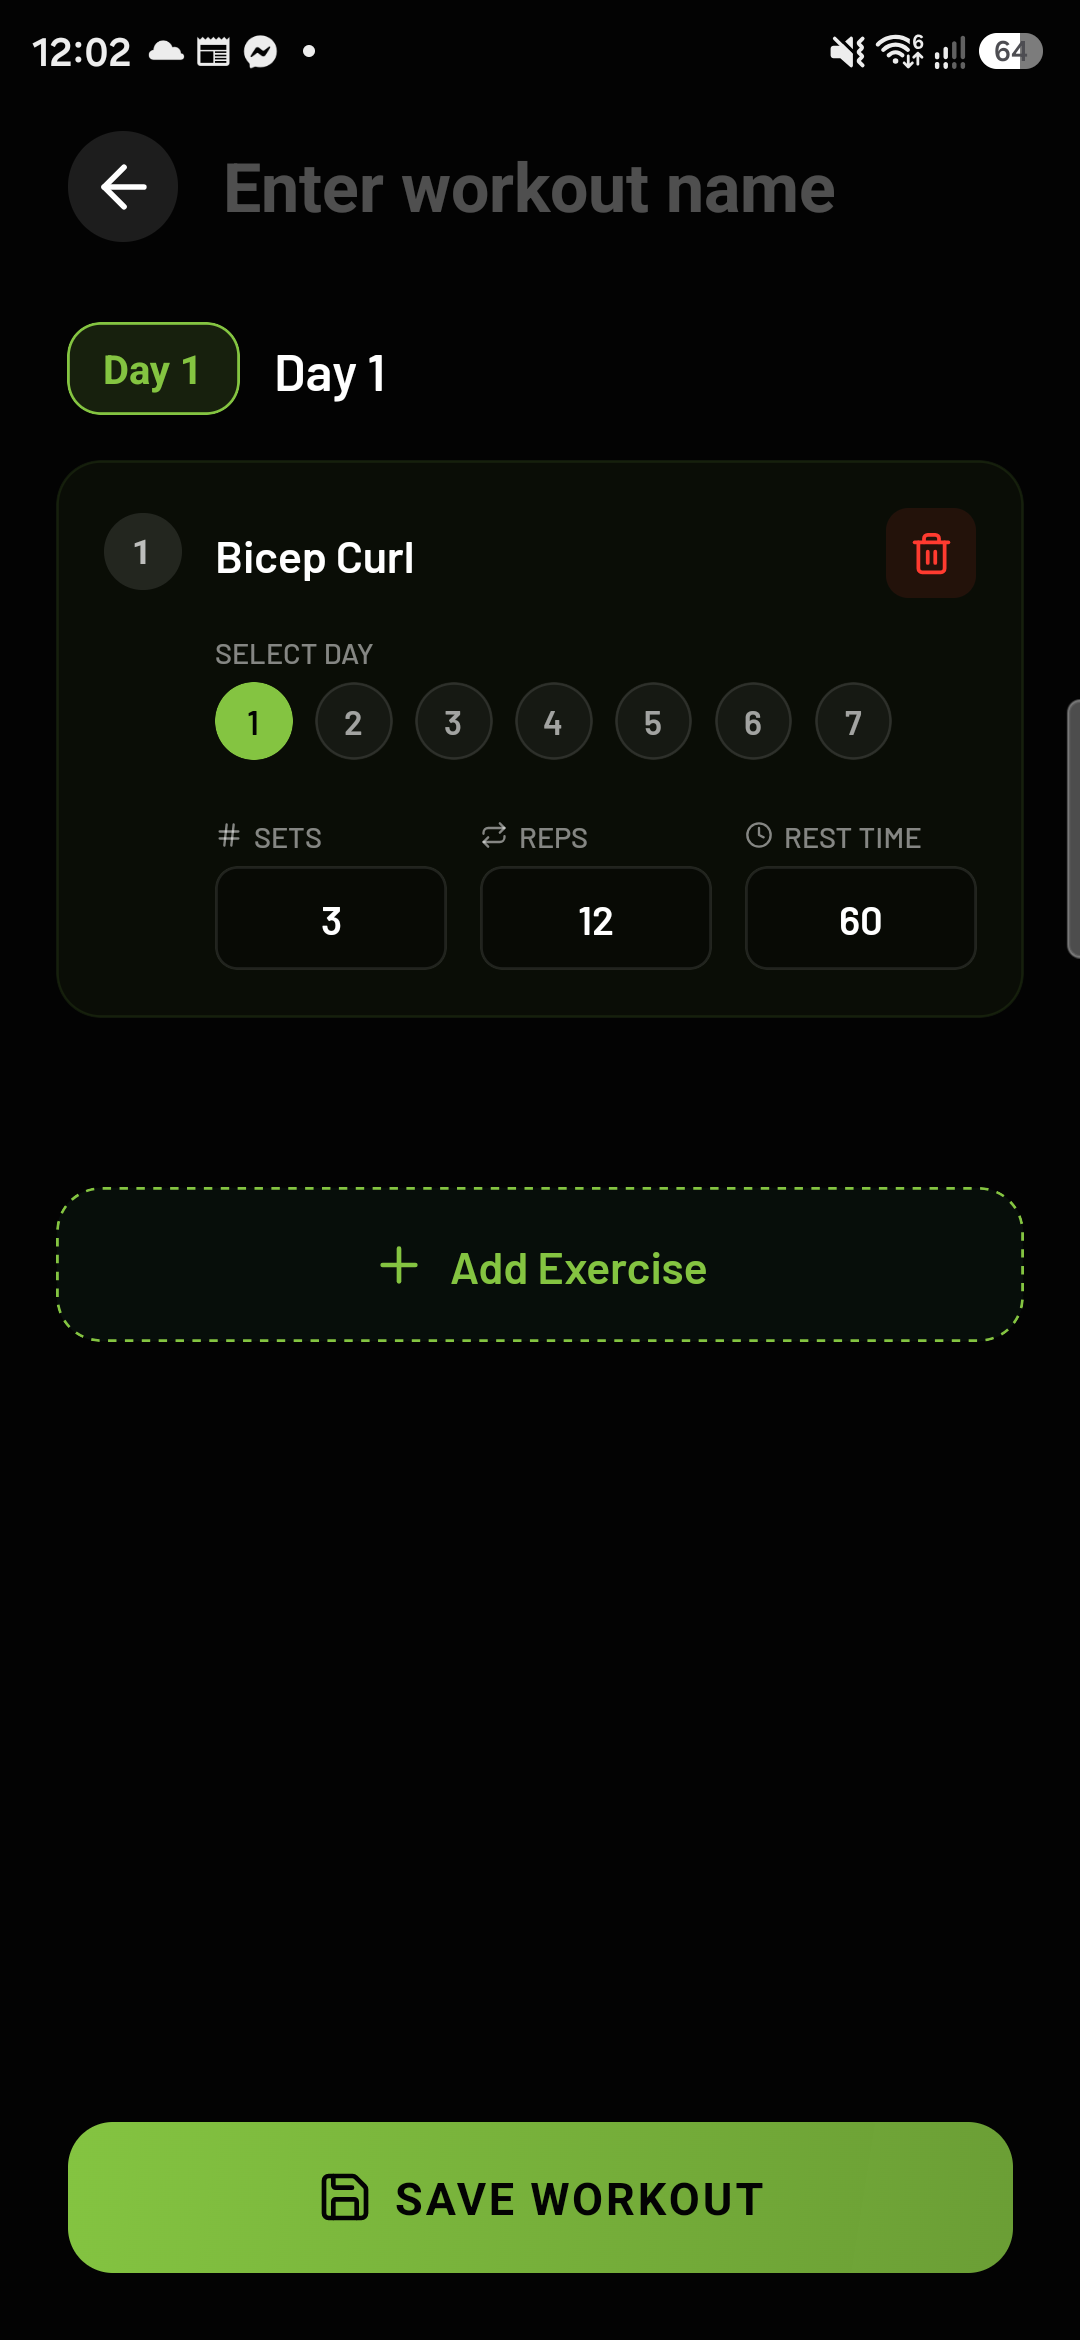
\includegraphics[width=\linewidth]{figures/screenshots/client-workout-builder.png}
\par\smallskip{\footnotesize b) Workout-builder form\par}
\end{minipage}
\caption{Interface captures: exercise detail and workout configuration; execution checks remain separate.}
\label{fig:ui-workout-configuration}
\end{figure}

Figure~\ref{fig:ui-workout-selection-save} adds the exercise selector and the created disposable workout card. The fixture was later deleted during QA; its presence demonstrates the recorded creation path, not a complete active-session or offline test.

\begin{figure}[H]
\centering
\begin{minipage}[t]{.31\linewidth}
\centering

\includegraphics[width=\linewidth]{figures/screenshots/client-exercise-selection.png}
\par\smallskip{\footnotesize a) Exercise selector\par}
\end{minipage}
\hspace{0.025\linewidth}
\begin{minipage}[t]{.31\linewidth}
\centering
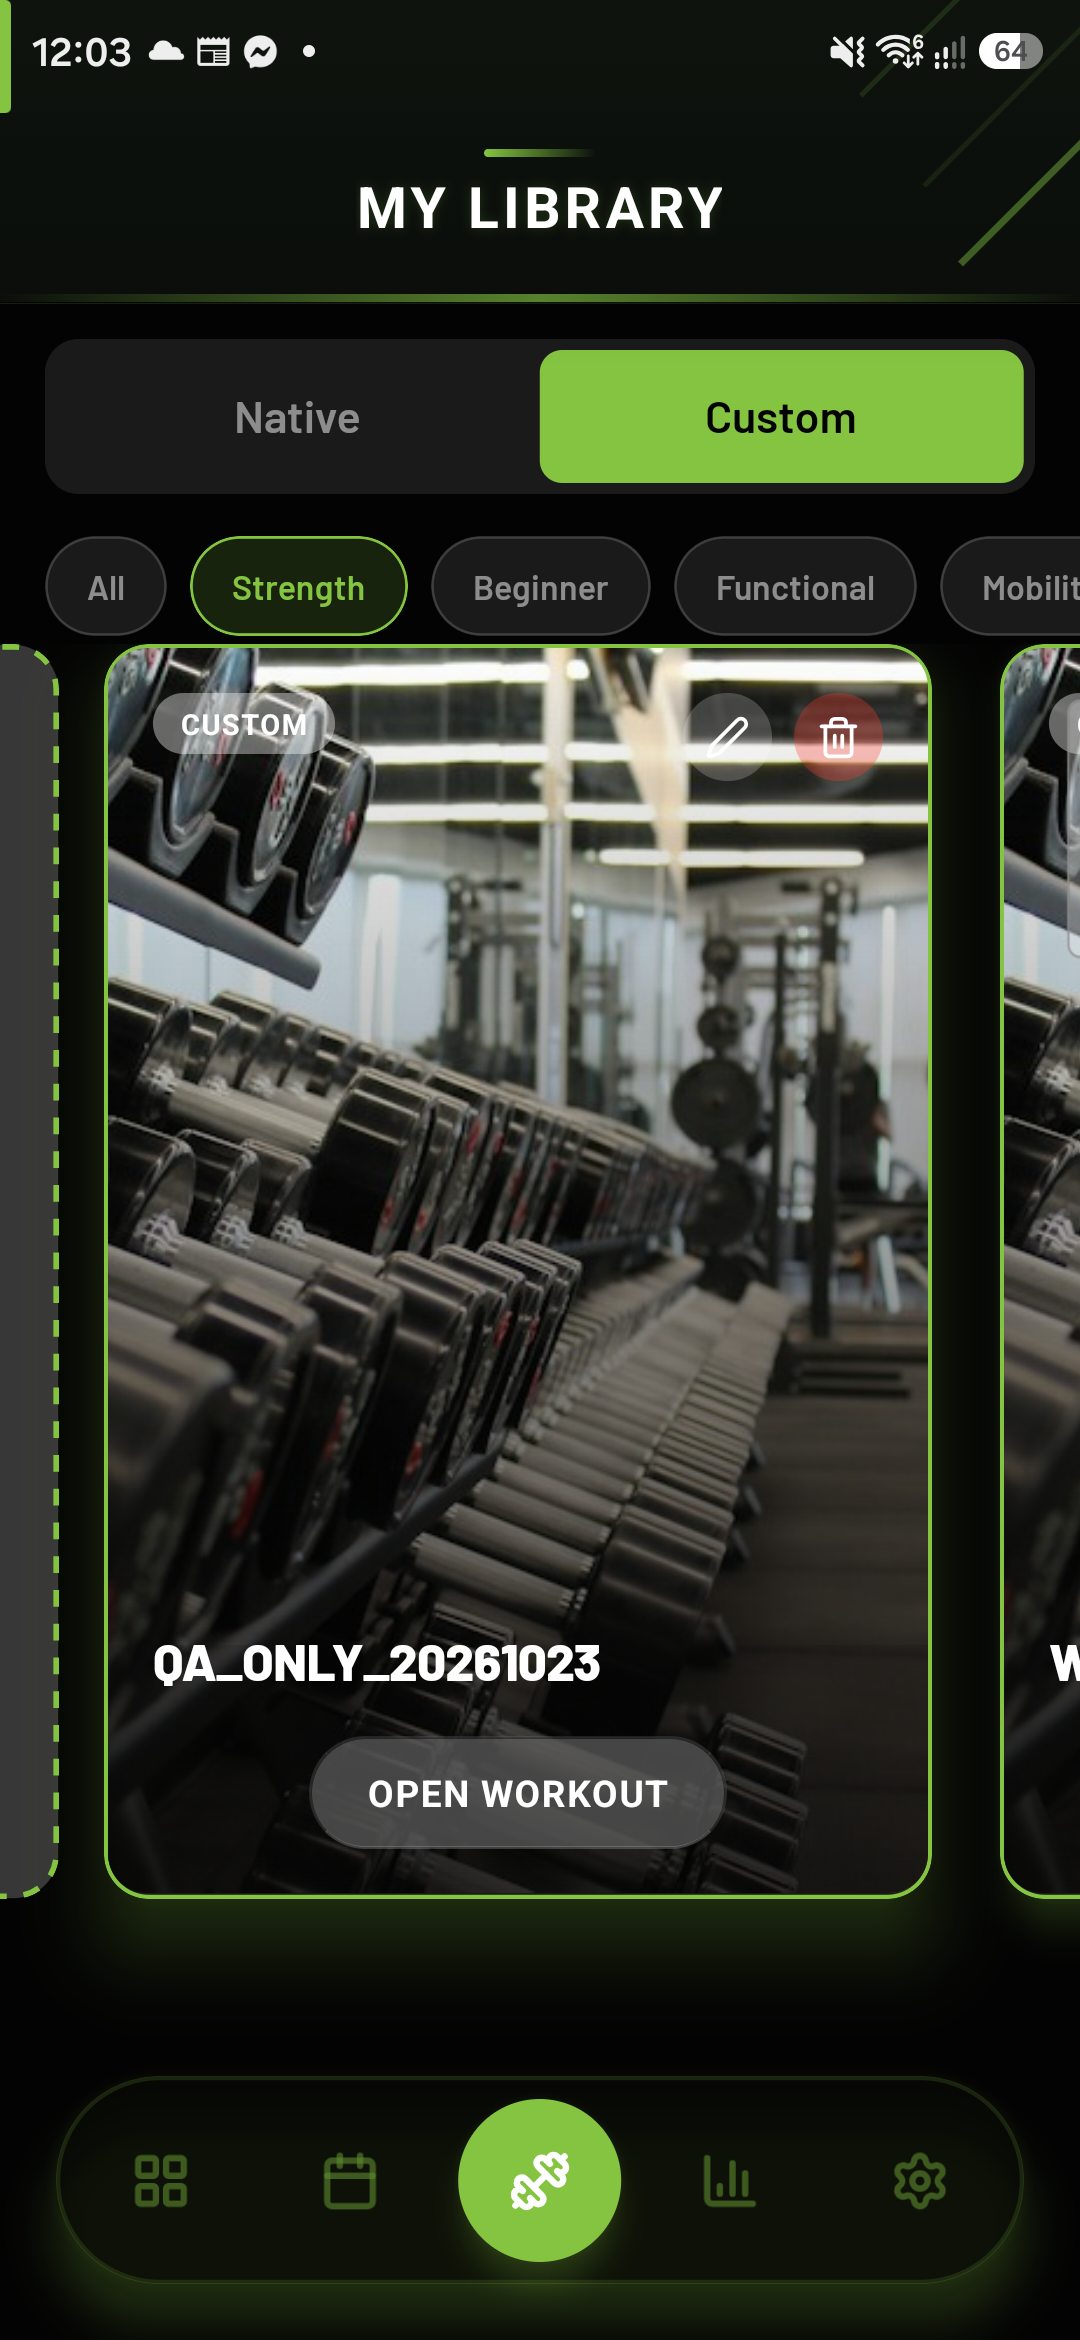
\includegraphics[width=\linewidth]{figures/screenshots/client-created-workout.png}
\par\smallskip{\footnotesize b) Created QA workout card\par}
\end{minipage}
\caption{Client workout walkthrough: exercise selection and the created disposable workout in the custom catalog.}
\label{fig:ui-workout-selection-save}
\end{figure}

\subsection{Offline Workout Resiliency and Fault-Tolerant Queue}

A critical architectural challenge encountered during gym testing is network instability. Physical gym environments frequently feature thick reinforced concrete walls or subterranean weight rooms where cellular connectivity drops completely. Without proper handling, finishing a session in an offline state results in lost workout telemetry, user frustration, and broken streaks.


To ensure bulletproof reliability, GoFit introduces an optimistic offline workout queue service \seqsplit{(GoFitMobile/src/services/offlineQueue.ts).} When the user completes a session and the API request fails due to network unreachability, the application intercepts the error, persists the session payload securely


into local AsyncStorage, and presents immediate positive feedback so the user's flow is uninterrupted. Concurrently, a NetInfo network listener registered at the application root (App.tsx) detects when Internet connectivity is re-established. The queue processor then automatically dequeues, synchronizes, and confirms the stored workout sessions against Supabase in the background with deduplication safeguards.


\subsection{Exercise Video Storage and Playback}

The administration panel implements a media-upload path to Cloudflare R2 using an S3-compatible client. The upload service sends the file as an object and returns a URL constructed from the configured public base URL. The mobile exercise-detail screen reads the stored \texttt{video\_url}; this separates the media reference from the binary object. The upload implementation alone does not establish a complete inventory of uploaded videos, project-specific bandwidth charges or comparative delivery performance.


\texttt{ExerciseDetailScreen} uses \texttt{expo-video} to load the stored URL, configures looping and tracks playback position. Custom controls implement play/pause, seeking and fullscreen entry, while player-status events update loading and error states. These source-defined mechanisms do not constitute measurements of decoding mode, buffering behavior, playback smoothness or energy consumption.

The retained Android observation, EXERCISE-04, records rendered video frames, a five-second timeline and reachable play/pause and fullscreen entry. It also records inconsistent control-tap responses and fullscreen-control visibility issues. No startup-latency, rebuffering, frame-rate or battery-consumption benchmark is retained. The playback scenario therefore remains Partial in the Sprint 1 validation matrix (Table~\ref{tab:pdf-42-21}); reliable performance across devices and network conditions requires further testing.


The workout-session interactions and persistence boundaries are detailed in Figures~\ref{fig:seq_workout_ssd}, \ref{fig:seq_workout_detailed} and \ref{fig:seq_workout_offline}. Their associated use-case description distinguishes prescribed repetitions from entered weights and completion flags, and remote completion from a pending local retry.

\section{Sprint Tests}

This matrix reconciles the original test identifiers with the retained 22--24 October evidence; it is not a recovered sprint-period execution log. Expected outcomes remain test criteria. Partial denotes narrower observations, Pending denotes an unverified full scenario, and Scoped pass applies only to the named sandbox case. M references identify Table~\ref{tab:implementation-evidence} and its detailed index; C, A, P and S identify the evidence package in Section~\ref{sec:qa-evidence}. No missing attachment is replaced by an assumed success.


\begingroup
\scriptsize
\setlength{\tabcolsep}{2pt}
\renewcommand{\arraystretch}{1.20}
\setlength{\LTpre}{5pt}
\setlength{\LTpost}{10pt}
\begin{longtable}{|L{1.20cm}|L{1.50cm}|L{1.60cm}|L{1.60cm}|L{1.80cm}|L{1.80cm}|L{1.65cm}|L{1.35cm}|L{2.00cm}|}
\caption{Sprint validation matrix}\label{tab:pdf-42-21} \\
\hline
\rowcolor{entetetab}
Test ID & Feature & Scenario & Preconditions & Steps & Expected & Actual & Status & Evidence \\ \hline
\endfirsthead
\hline
\rowcolor{entetetab}
Test ID & Feature & Scenario & Preconditions & Steps & Expected & Actual & Status & Evidence \\ \hline
\endhead
S1-T01 & Authentication & Existing-account sign-in & Existing test account & Sign in; reopen app & Protected client route & Observed scoped access & Partial & M01; C AUTH-01--04; fresh registration and refresh not verified \\ \hline
S1-T02 & Onboarding & Fresh six-screen profile save & New client fixture & Complete full form; read back & Answers persisted remotely & Fresh flow not run & Pending & M02; saved-profile views do not validate new onboarding \\ \hline
S1-T03 & Workout session & Weights and completion save & Existing remote session & Record weights; finish; read back & Existing session updated & Full completion not retained & Pending & M05; no RPE or separate WorkoutSet table \\ \hline
S1-T04 & Rest timer & Countdown and background alerts & Active workout & Complete set; lock; observe & Countdown and configured feedback & Informal user confirmation only & Pending & M05; QA-02 lacks retained timing\slash{}background evidence \\ \hline
S1-T05 & Offline queue & Existing-session completion replay & Remote session; disconnected & Finish; reconnect; compare row & Queued UPDATE replayed once & Not exercised with readback & Pending & M06; final QA-03 \\ \hline
S1-T06 & Exercise media & Play exercise demonstration & Network and media URL & Open detail; start playback & Playable demonstration & Detail\slash{}media observations partial & Partial & M03; C EXERCISE-01--04; smoothness\slash{}decoding not measured \\ \hline
\end{longtable}
\endgroup

\section{Progress Tracking and Evidence Limits}

The retained backlog provides planned tasks and estimates, but no dated series of remaining work, scope changes or accepted completions is available for this report scope group. A burn-down chart and measured velocity cannot be reconstructed from the current source tree or later QA outcomes. No chart is therefore presented as evidence of sprint performance. The validation matrix reports the narrower implementation and execution evidence instead.


\phantomsection
\section*{Conclusion}

This chapter described authentication, client onboarding, workout prescriptions, embedded execution snapshots and rest-timer configuration. The sequences distinguish remote session creation, successful completion updates and conditional offline retry. Retained existing-account observations do not establish fresh onboarding, controlled background timer behavior or complete offline reconciliation. These limits remain visible in the sprint matrix and Table~\ref{tab:implementation-evidence}. The next chapter examines progress, measurements and nutrition.


\chapter{Sprint 2}


\phantomsection
\section*{Introduction}
\addcontentsline{toc}{section}{Introduction}

The Sprint 2 scope concerns progress history, nutrition and saved food records, measurement capture and review, recommendation requests and reminder configuration. It examines the corresponding source paths and distinguishes them from unverified barcode execution, fresh AI measurement accuracy, recommendation generation and scheduled delivery.


This chapter examines the scope designated Sprint 2 through planned tasks, cumulative domain views, selected use cases and interaction sequences, implementation descriptions and reconciled validation criteria. The models project the inspected implementation, while the retained October observations are later evidence. The closing management subsection states the limits of available progress-tracking data.


\section{Needs Assessment}

The sprint needs were selected from the prioritized product backlog according to dependency order, business value, and architectural feasibility. The following table provides a comprehensive decomposition of each user story into technical modeling, implementation, and testing subtasks.


The Sprint 2 objective is to connect workout history with progress, nutrition and assisted self-monitoring. The backlog records development and testing targets; its presence does not establish complete implementation or successful execution.


\subsection{Sprint Backlog}

\begingroup
\scriptsize
\setlength{\tabcolsep}{3pt}
\renewcommand{\arraystretch}{1.20}
\setlength{\LTpre}{5pt}
\setlength{\LTpost}{10pt}
\begin{longtable}{|L{1.20cm}|L{2.00cm}|L{5.40cm}|L{1.80cm}|L{4.00cm}|}
\caption{Sprint 2 backlog decomposition}\label{tab:pdf-45-22} \\
\hline
\rowcolor{entetetab}
ID US & As & User Story & Id task & Task \\ \hline
\endfirsthead
\hline
\rowcolor{entetetab}
ID US & As & User Story & Id task & Task \\ \hline
\endhead
US-4.1 & User & Capture front/side photos and obtain AI-assisted body measurements using on-device MediaPipe CV & T4.1.1 & Model BodyMeasurement entity, MediaPipe 33 pose landmarks mapping, and height anchor ratio formulas. \\ \hline
US-4.1 & User & Capture front/side photos and obtain AI-assisted body measurements using on-device MediaPipe CV & T4.1.2 & Implement CameraCaptureScre en, MediaPipe BlazePose \& Selfie Segmentation processing, and MeasurementRevie wScreen. \\ \hline
US-4.1 & User & Capture front/side photos and obtain AI-assisted body measurements using on-device MediaPipe CV & T4.1.3 & Test landmark detection confidence thresholds, low-lighting warnings, and editable manual override sheet. \\ \hline
US-4.2 & User & Track daily nutrition, search food items, scan barcodes via OpenFoodFacts, and \seqsplit{filterallergens/dislikes} & T4.2.1 & Design NutritionLog, FoodItem, and UserDietaryPreferences schema with allergen exclusion filtering. \\ \hline
US-4.2 & User & Track daily nutrition, search food items, scan barcodes via OpenFoodFacts, and \seqsplit{filterallergens/dislikes} & T4.2.2 & Develop NutritionScreen, BarcodeScannerScre en, MacroRings component, and OpenFoodFacts API service. \\ \hline
US-4.2 & User & Track daily nutrition, search food items, scan barcodes via OpenFoodFacts, and \seqsplit{filterallergens/dislikes} & T4.2.3 & Test macro calculation (protein/carbs/fat/c alories), barcode product resolution, and disliked ingredient SQL filters. \\ \hline
US-4.3 & User & Track physical progress over time with interactive metric charts, volume graphs, and progress photos & T4.3.1 & Model ProgressPhoto storage bucket paths and historical analytics aggregation queries. \\ \hline
US-4.3 & User & Track physical progress over time with interactive metric charts, volume graphs, and progress photos & T4.3.2 & Implement ProgressScreen with Victory Native charts, 1RM progression curves, and side-by-side photo comparison slider. \\ \hline
US-4.3 & User & Track physical progress over time with interactive metric charts, volume graphs, and progress photos & T4.3.3 & Test empty-state visualizations, date-range filtering, and Cloudflare R2 /Supabase Storage photo retrieval. \\ \hline
US-4.4 & User & Receive automated workout reminders, hydration alerts, and adaptive AI workout recommendations via Groq LLaMA-3.3 & T4.4.1 & Design Edge Function \seqsplit{ai-workout-recommendation} prompt engineering with user muscle fatigue context. \\ \hline
US-4.4 & User & Receive automated workout reminders, hydration alerts, and adaptive AI workout recommendations via Groq LLaMA-3.3 & T4.4.2 & Implement NotificationSettingsS creen, Expo push notification scheduling, and AI recommendation card. \\ \hline
US-4.4 & User & Receive automated workout reminders, hydration alerts, and adaptive AI workout recommendations via Groq LLaMA-3.3 & T4.4.3 & Test notification permission handshakes, Groq API token streaming, and fallback to rule-based templates on timeout. \\ \hline
\end{longtable}
\endgroup

This backlog records planned scope rather than completed tests. US-4.1 maps to BodyMeasurement and the capture/review/save sequences; the inspected Android path is not evidence of numerical accuracy or equivalent iOS support. US-4.2's NutritionLog and UserDietaryPreferences are planning terms: the implemented model uses MealLog, FoodItem, NutritionGoals and profile collections. Name-based exclusions are distinct from ingredient-safety verification. US-4.3 maps to independent ProgressPhoto records and session-derived statistics; named chart libraries, progression curves and a comparison slider require their own implementation and execution evidence. US-4.4 maps to notification preferences and recommendation services, not a guaranteed notification schedule, streamed response or validated timeout fallback. See Table~\ref{tab:sprint-traceability}.

\subsection{Sprint Class Diagram}

The Sprint 2 cumulative domain model is presented in two complementary views. Figure~\ref{fig:class_sprint2_foundation} retains all eight concepts and relationships of the Sprint 1 foundation. Figure~\ref{fig:class_sprint2} extends that foundation with body measurements, progress photos, food items, meal logs, nutrition goals, and embedded notification preferences. Earlier profile attributes remain part of the model; the extension view expands only its dietary fields. Each measurement record stores reviewed values and estimation metadata, while progress photos are independent records; no saved photo is required for each AI-assisted measurement. MealLog associates an account with a food item, date, meal category, and serving quantity, from which nutrient totals are calculated. Each account may have at most one NutritionGoals record. Dietary preferences, allergies, and dislikes are profile collections, while notification preferences are optional embedded configuration, distinct from local rest-timer settings. Training statistics are derived from session history, and accepted AI workout recommendations reuse the existing workout model. These views present the principal domain concepts rather than an exhaustive database schema.

\begin{figure}[H]
\centering
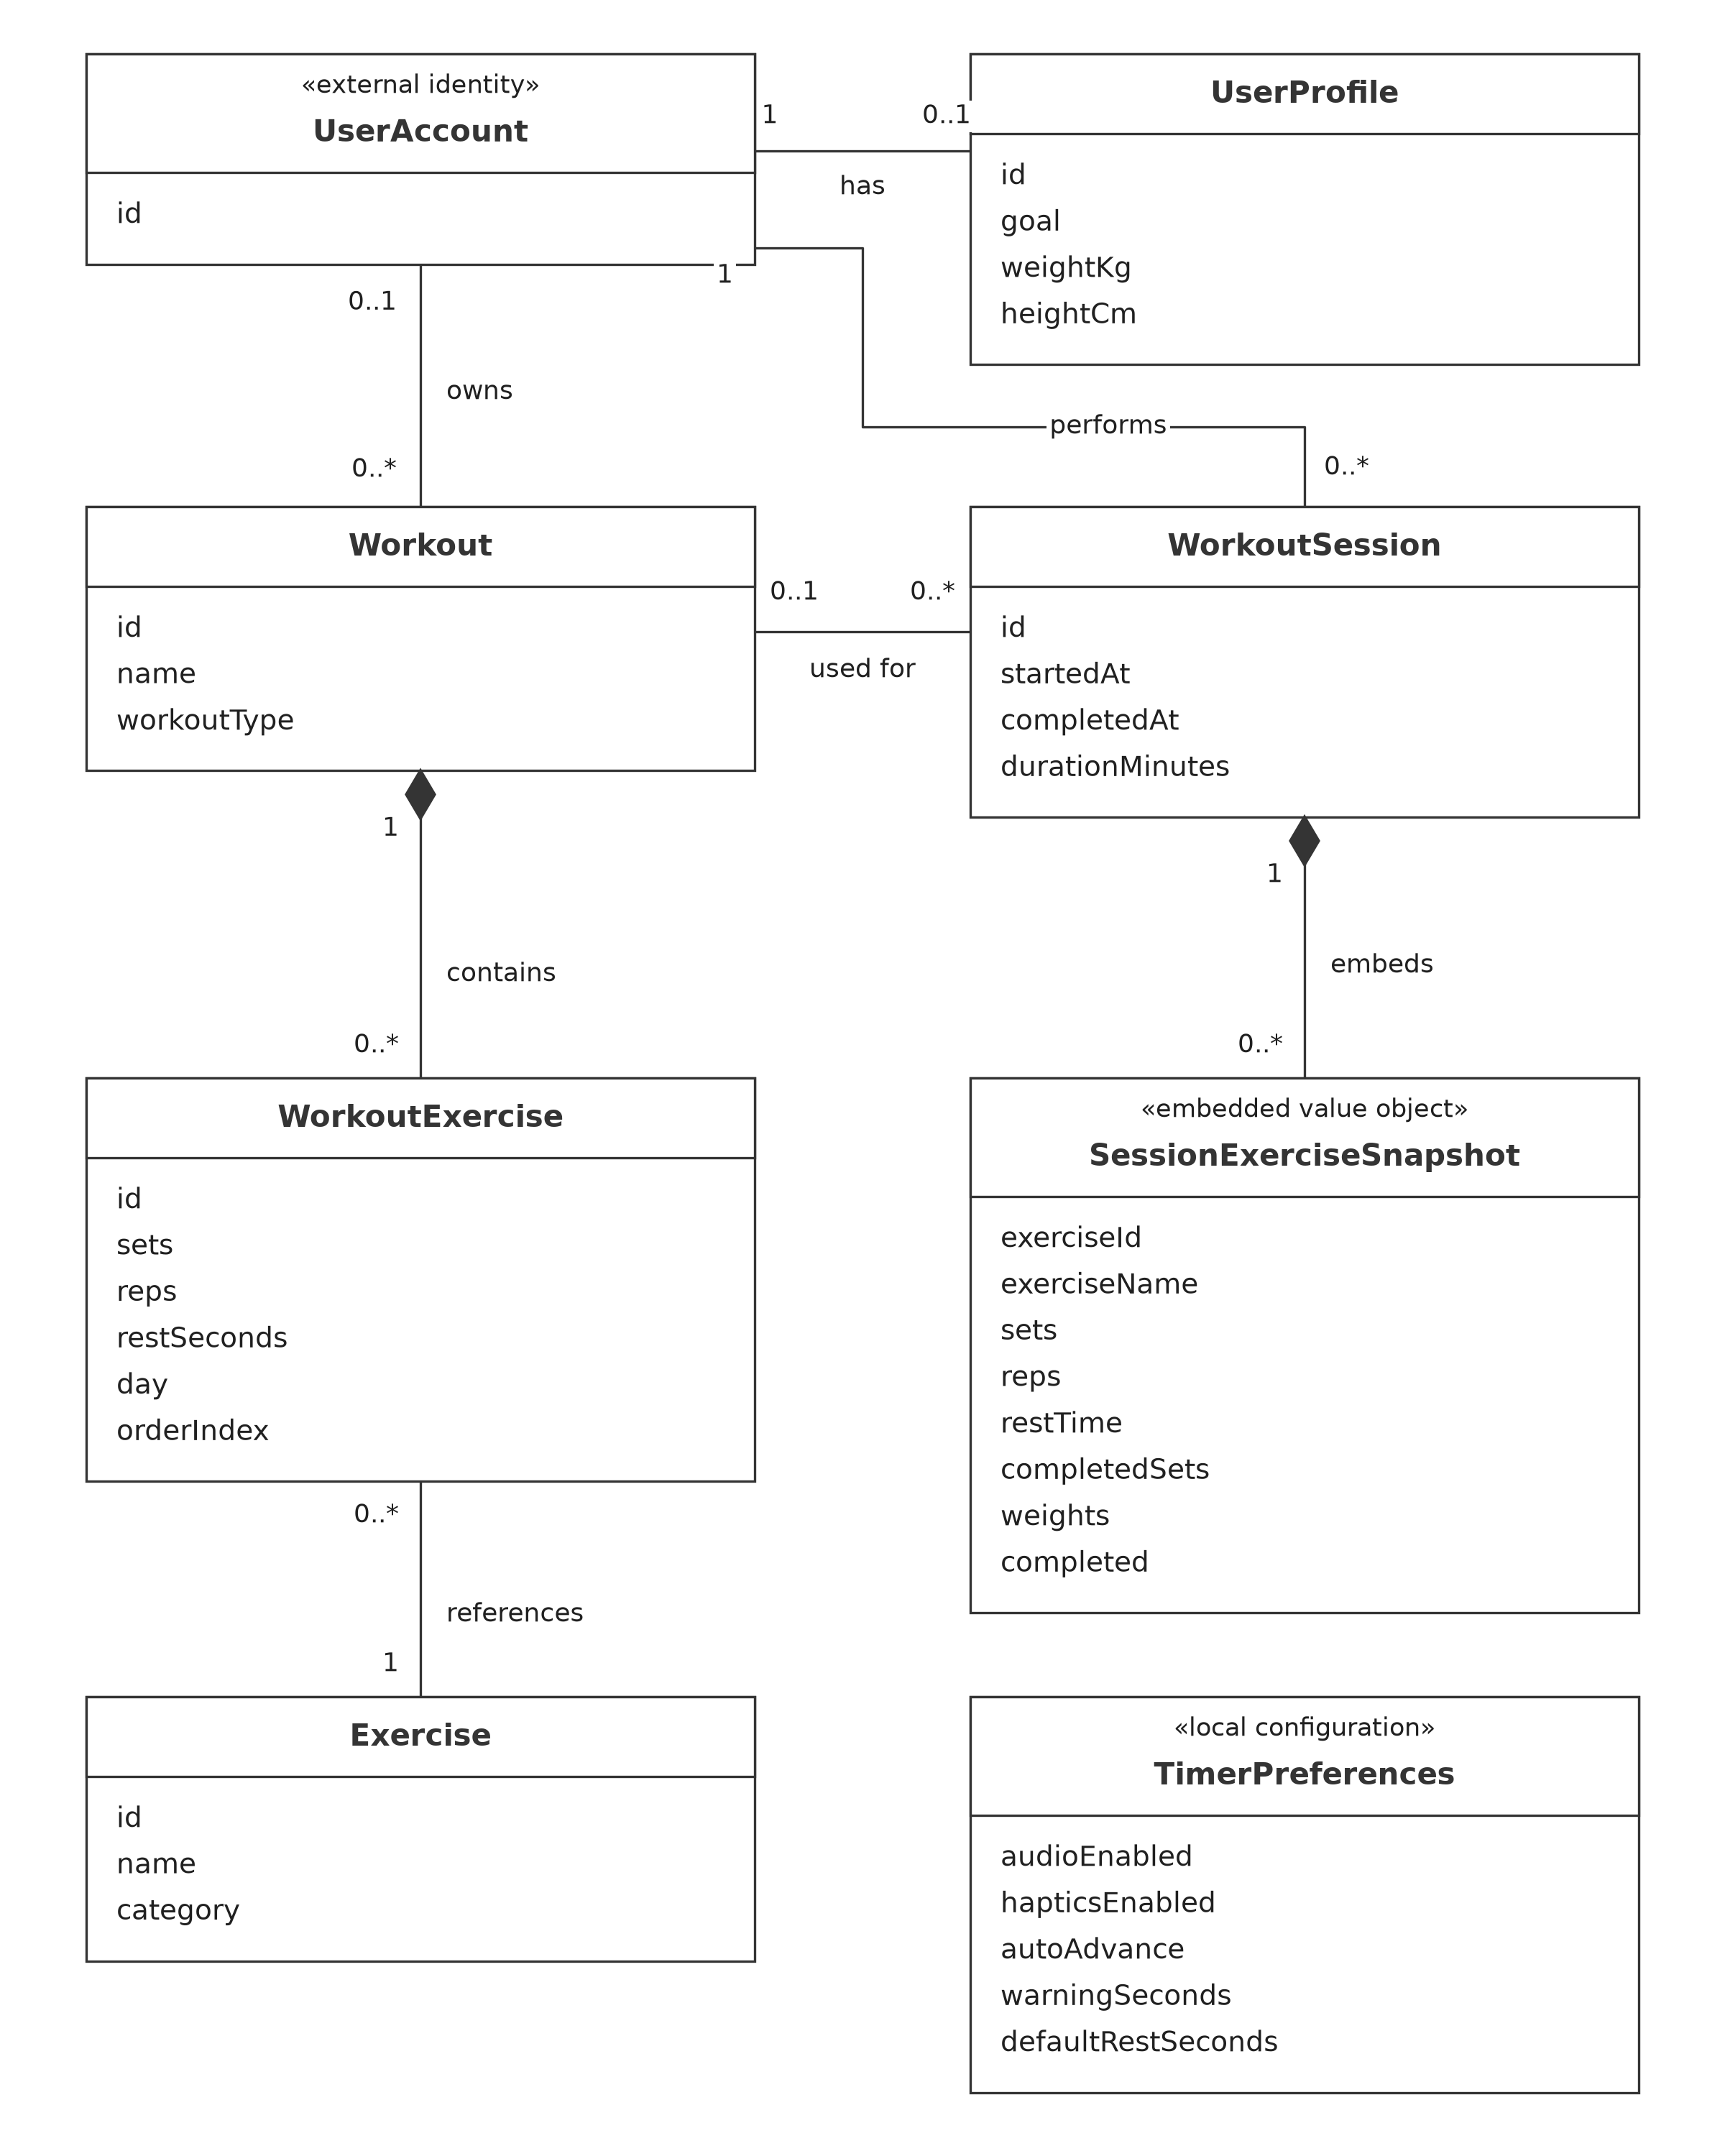
\includegraphics[width=0.88\linewidth]{figures/class_diagram_sprint1.png}
\caption{Sprint 2 cumulative domain model: retained workout foundation}
\label{fig:class_sprint2_foundation}
\end{figure}


\begin{figure}[H]
\centering
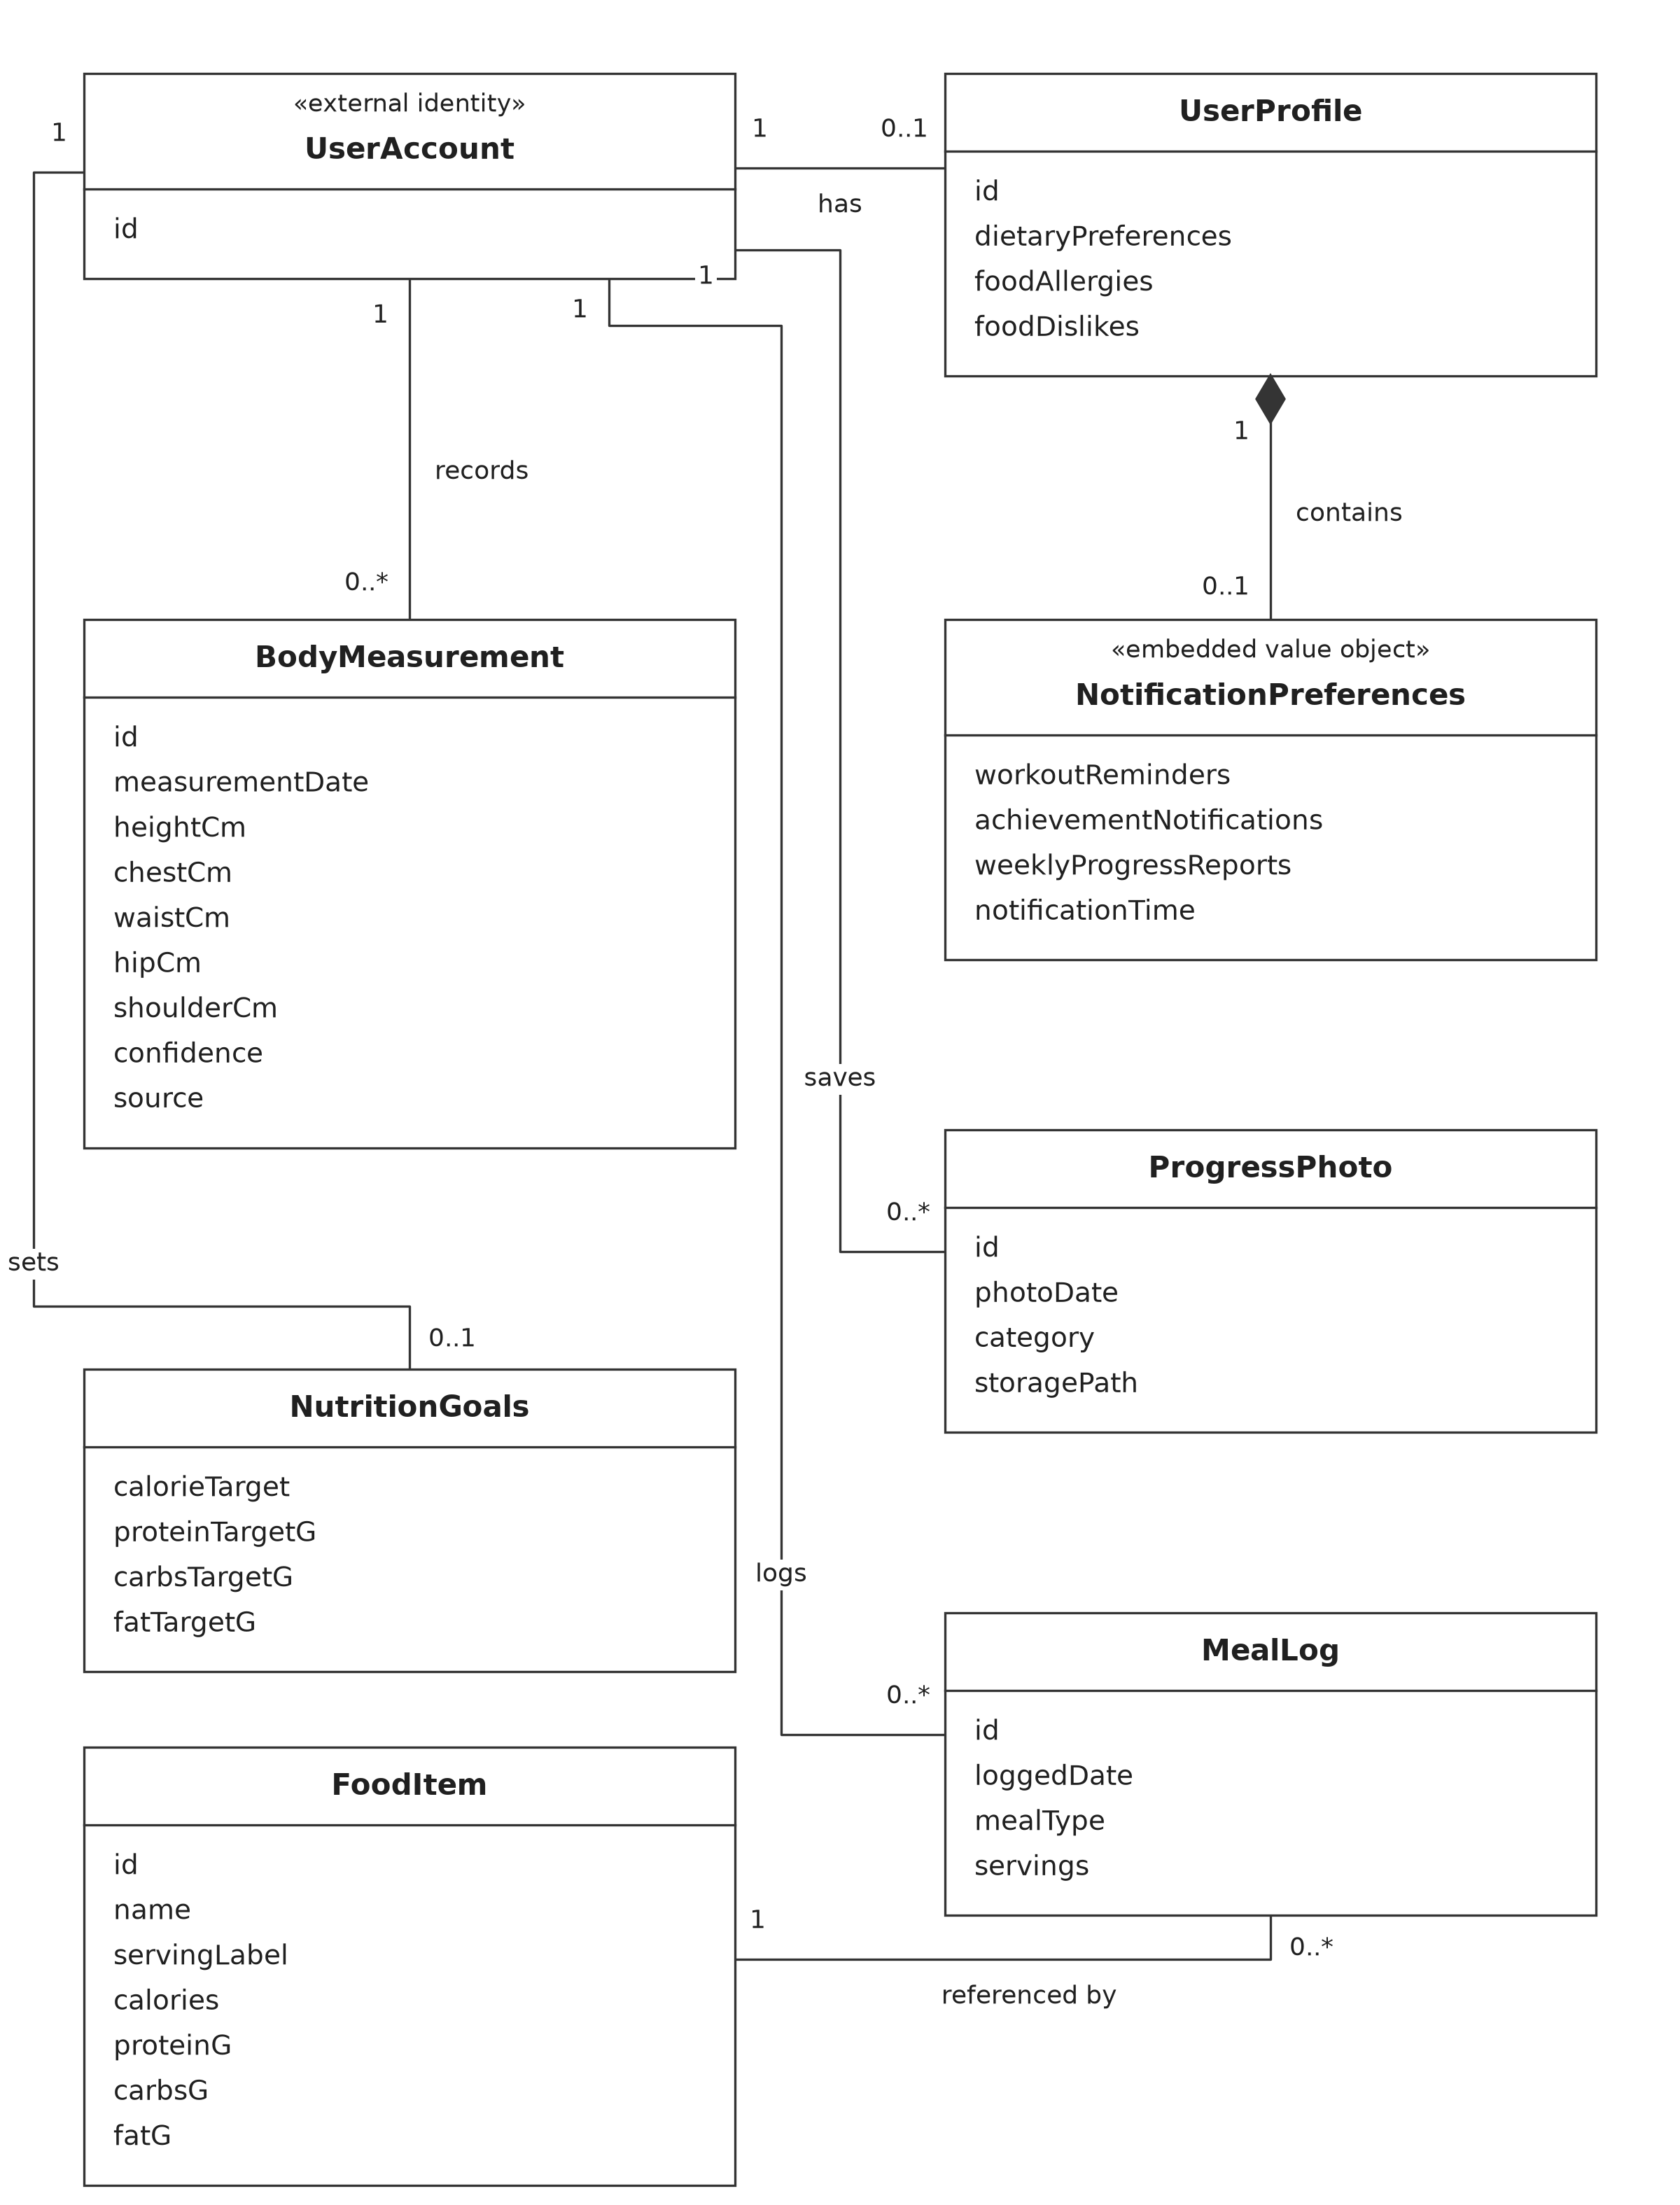
\includegraphics[width=0.95\linewidth]{figures/class_diagram_sprint2.png}
\caption{Sprint 2 cumulative domain model: profile, progress, and nutrition extensions}
\label{fig:class_sprint2}
\end{figure}

\section{Functional Specification of Requirements}

This section specifies the sprint use cases and analyzes the behavioral interactions between the participating actors and the GoFit platform.


\subsection{Refined Use Case Diagram of Sprint 2}

This view refines the Client's progress, nutrition, and assistance goals. It covers exercise-library browsing, progress review, measurement drafts, meal logging and nutrition targets, barcode lookup, dietary preferences, workout recommendations, and reminder configuration. Capture, processing, review, and saving belong to the measurement workflow; the draft terminology does not imply verified measurement accuracy. Dietary preferences and barcode lookup are shown as separate goals and do not establish an ingredient-safety guarantee. Platform dependencies and failure paths are examined in the corresponding implementation and sequence descriptions.


\begin{figure}[H]
\centering
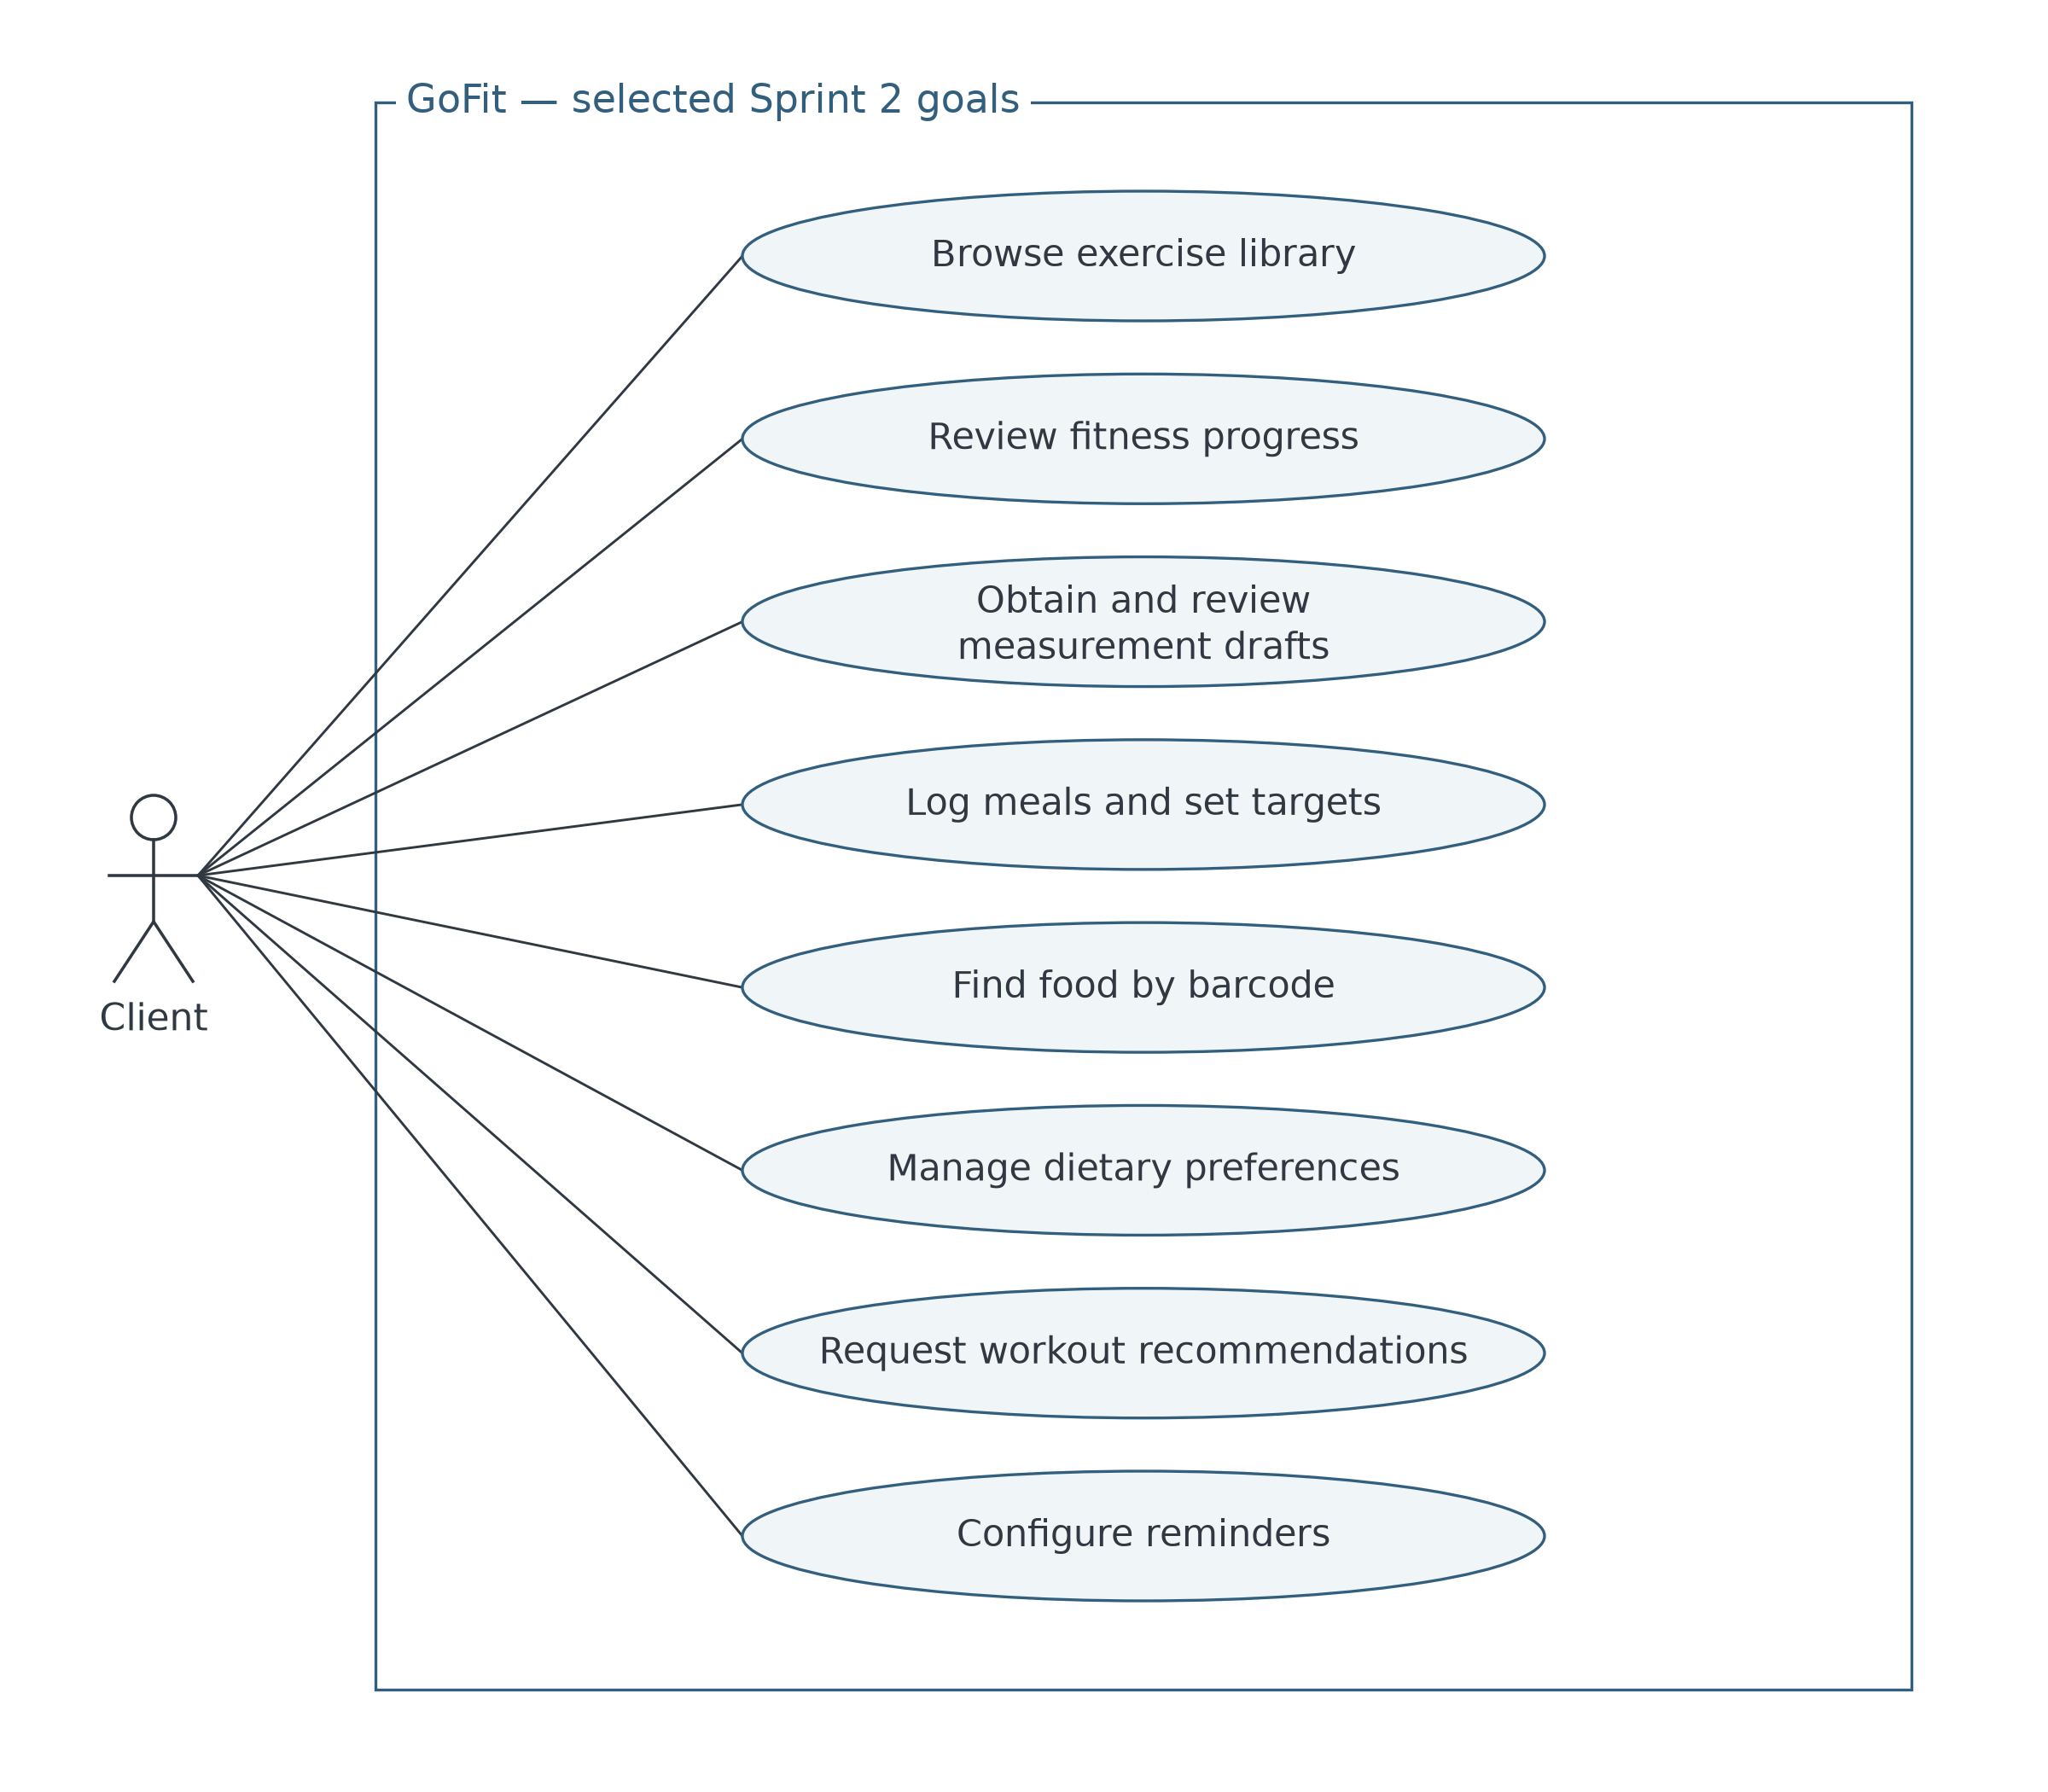
\includegraphics[width=0.92\linewidth]{figures/use_case_sprint2.png}
\caption{Selected client use cases associated with Sprint 2}
\label{fig:use_case_sprint2}
\end{figure}

\subsection{Use Case Analysis}

\subsubsection{Use case: Generate AI-assisted body measurements}

\begingroup
\footnotesize
\setlength{\tabcolsep}{3pt}
\renewcommand{\arraystretch}{1.20}
\setlength{\LTpre}{5pt}
\setlength{\LTpost}{10pt}
\begin{longtable}{|L{4.95cm}|L{10.05cm}|}
\caption{Textual description of use case: Generate AI-assisted body measurements}\label{tab:pdf-50-23} \\
\hline
\rowcolor{entetetab}
Field & Description \\ \hline
\endfirsthead
\hline
\rowcolor{entetetab}
Field & Description \\ \hline
\endhead
Use case & Generate AI-assisted body measurements \\ \hline
Primary actor & Mobile user \\ \hline
Preconditions & A valid height is available from the user profile, camera permission is granted for capture, and the installed build supports the required on-device inference modules. Saving additionally requires an authenticated user. \\ \hline
Postconditions & Following explicit review and a successful save, corrected chest, waist, hip, and shoulder values are stored in \texttt{body\_measurements}, together with height, model confidence, source, and original-estimate/correction metadata. The application reloads measurement history and returns to the introduction. Review records user acceptance or correction; it does not establish measurement accuracy. \\ \hline
Nominal scenario & 1. The user opens Body Measurement; the application reads height from the profile. 2. The user captures a front photo; capture validation must pass before proceeding to the side photo. 3. The accepted side capture triggers local pose-based estimation using height calibration and statistical depth priors. 4. Segmentation features are evaluated for eligible refinement or rescue of the base estimate. 5. The application displays editable draft values and quality warnings. 6. The user reviews or corrects the values and selects Save to progress. 7. Save checks and authentication succeed, the application inserts the measurement record, reloads history, and resets the capture flow. \\ \hline
Alternative scenario & 3.1. On Android, primary pose analysis attempts MediaPipe and falls back to MoveNet if that attempt fails. Other platforms select MoveNet for primary pose analysis, subject to native-runtime availability. 4.1. If segmentation fails or refinement is ineligible, the base result is retained; final quality checks can still prevent saving. 6.1. The user corrects individual draft values before saving. \\ \hline
Exception scenario & E.1. Capture validation rejects poor framing or pose quality and presents guidance for another capture. E.2. Camera permission is denied; the application displays a camera-access alert. E.3. Result errors, insufficient confidence, blocking warnings, or invalid edited values prevent saving. E.4. Missing authentication prompts sign-in; an insertion failure displays a save error. A separate history-load error can occur after an insertion succeeds. \\ \hline
\end{longtable}
\endgroup

\begin{figure}[H]
\centering
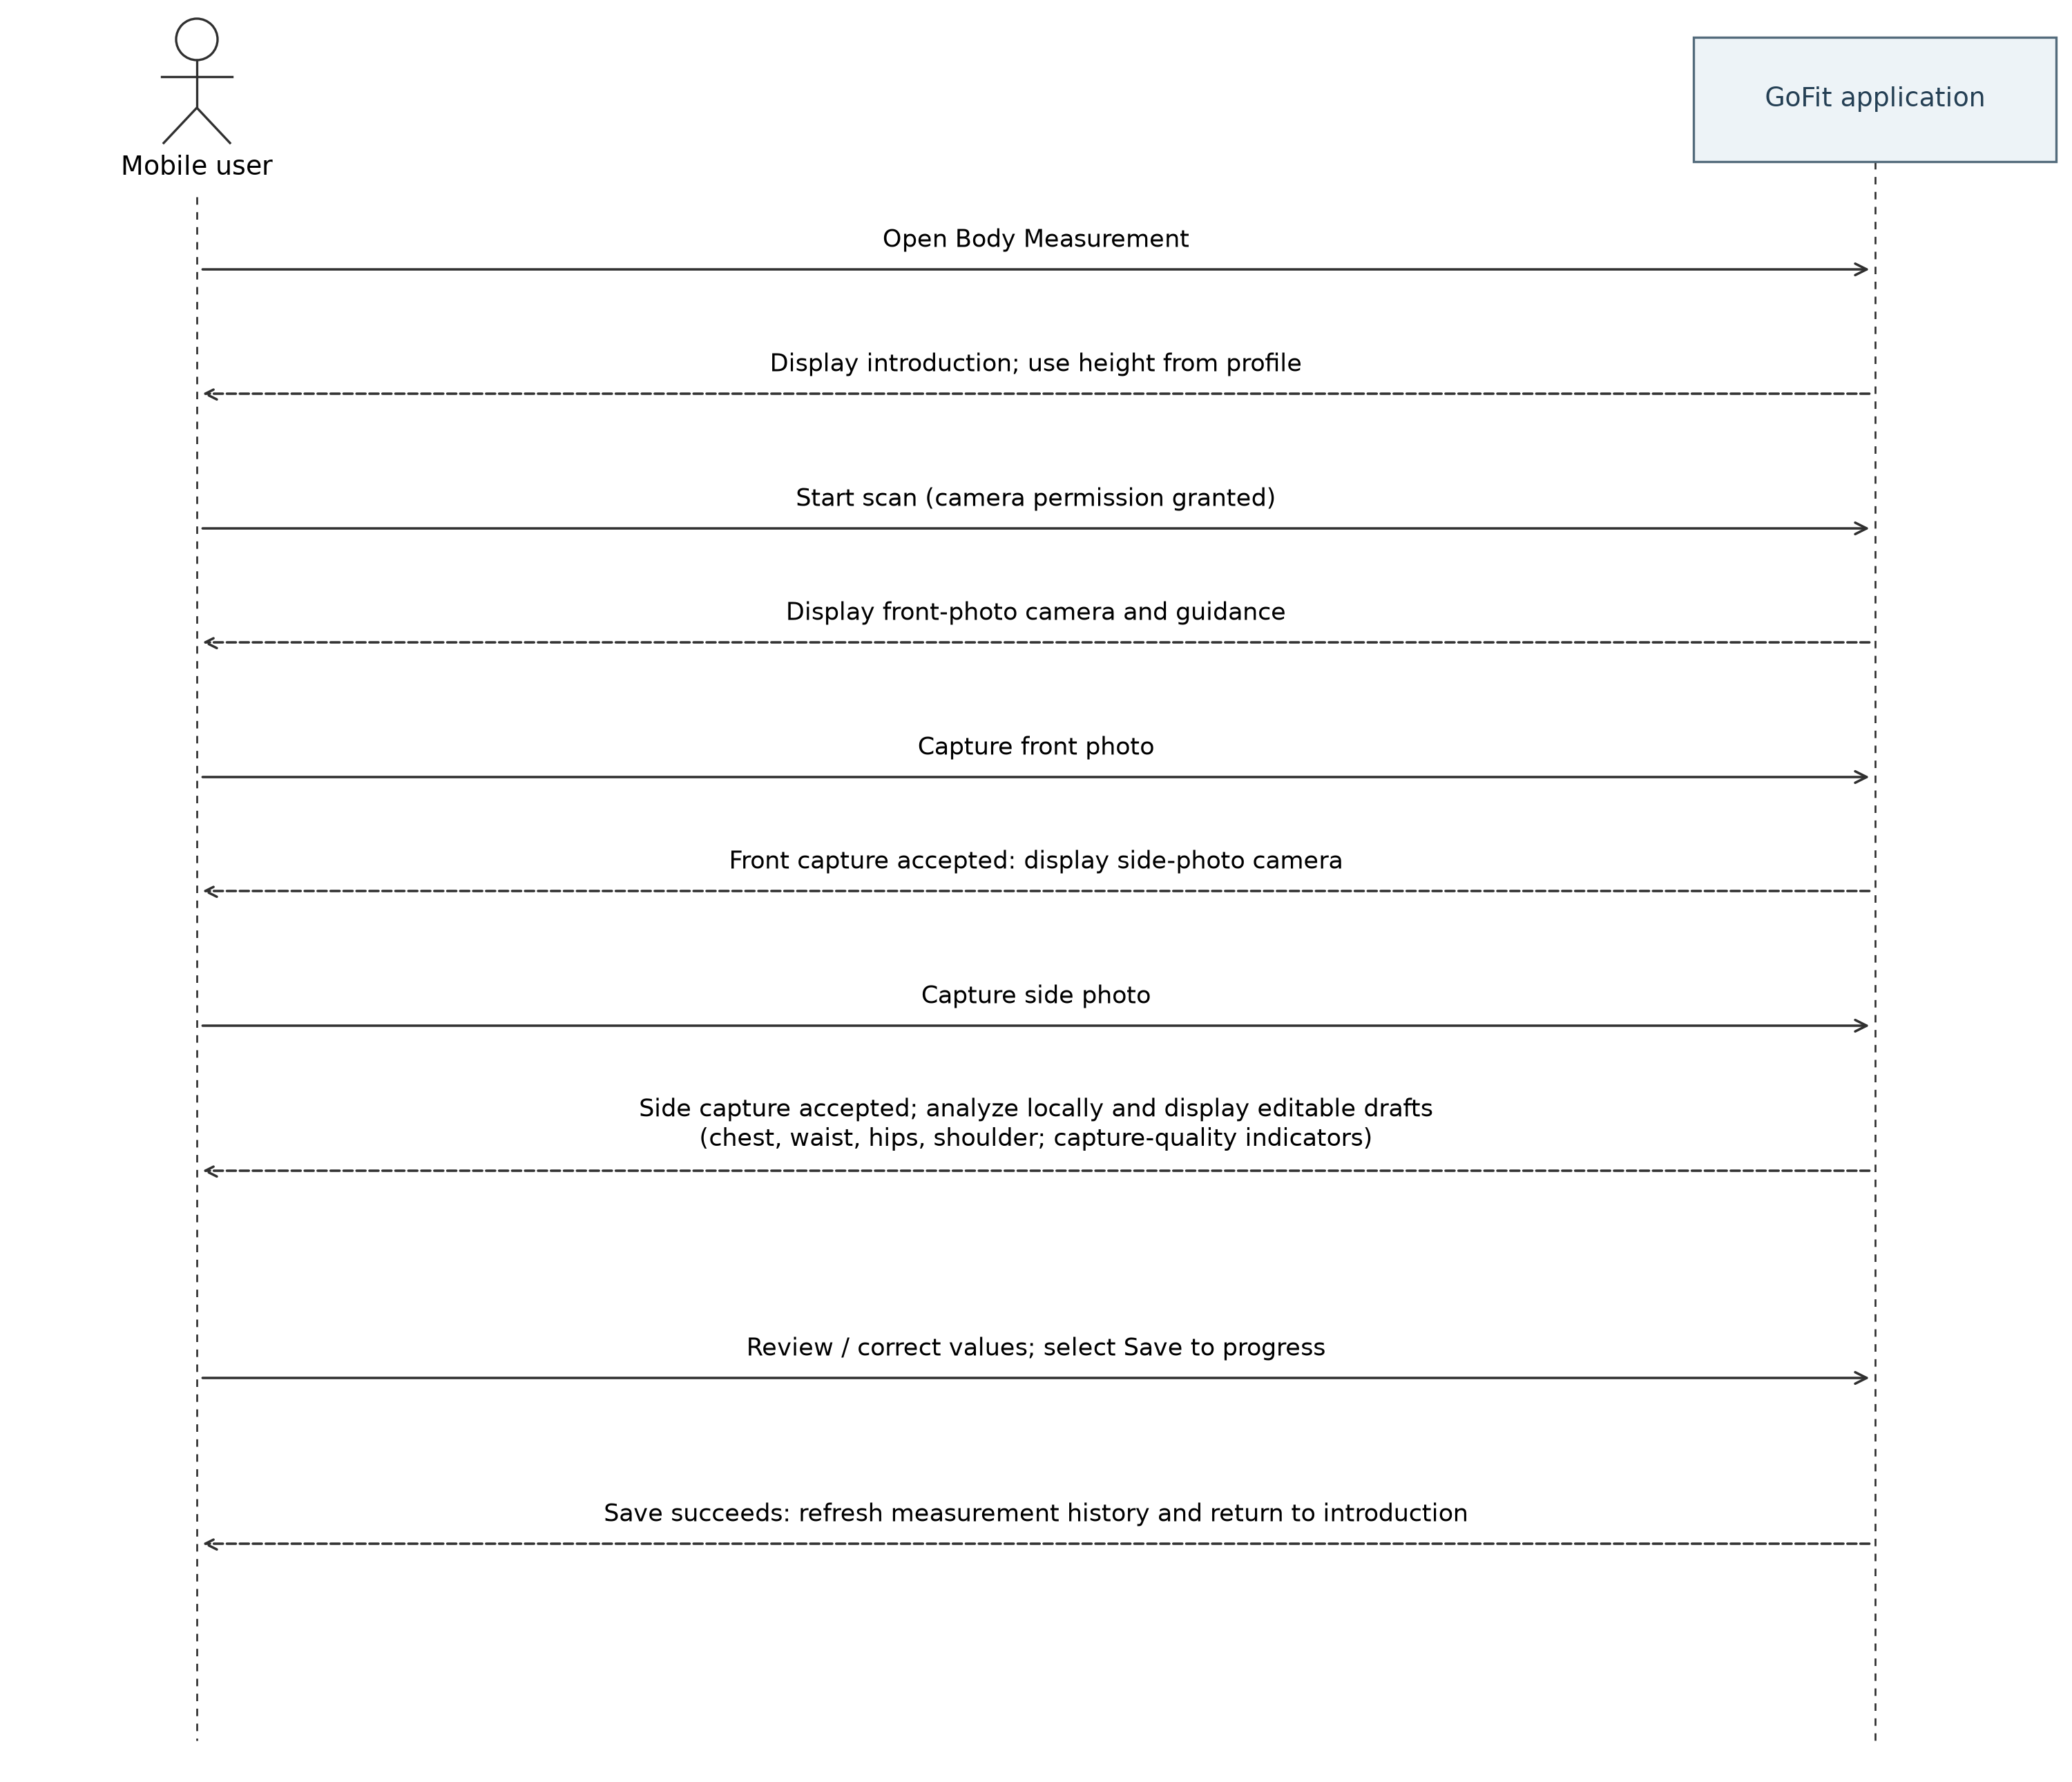
\includegraphics[width=0.92\linewidth]{figures/seq_measurement_ssd.png}
\caption{System sequence diagram: Body-measurement capture, review, and successful save}
\label{fig:seq_measurement_ssd}
\end{figure}

\begin{figure}[H]
\centering
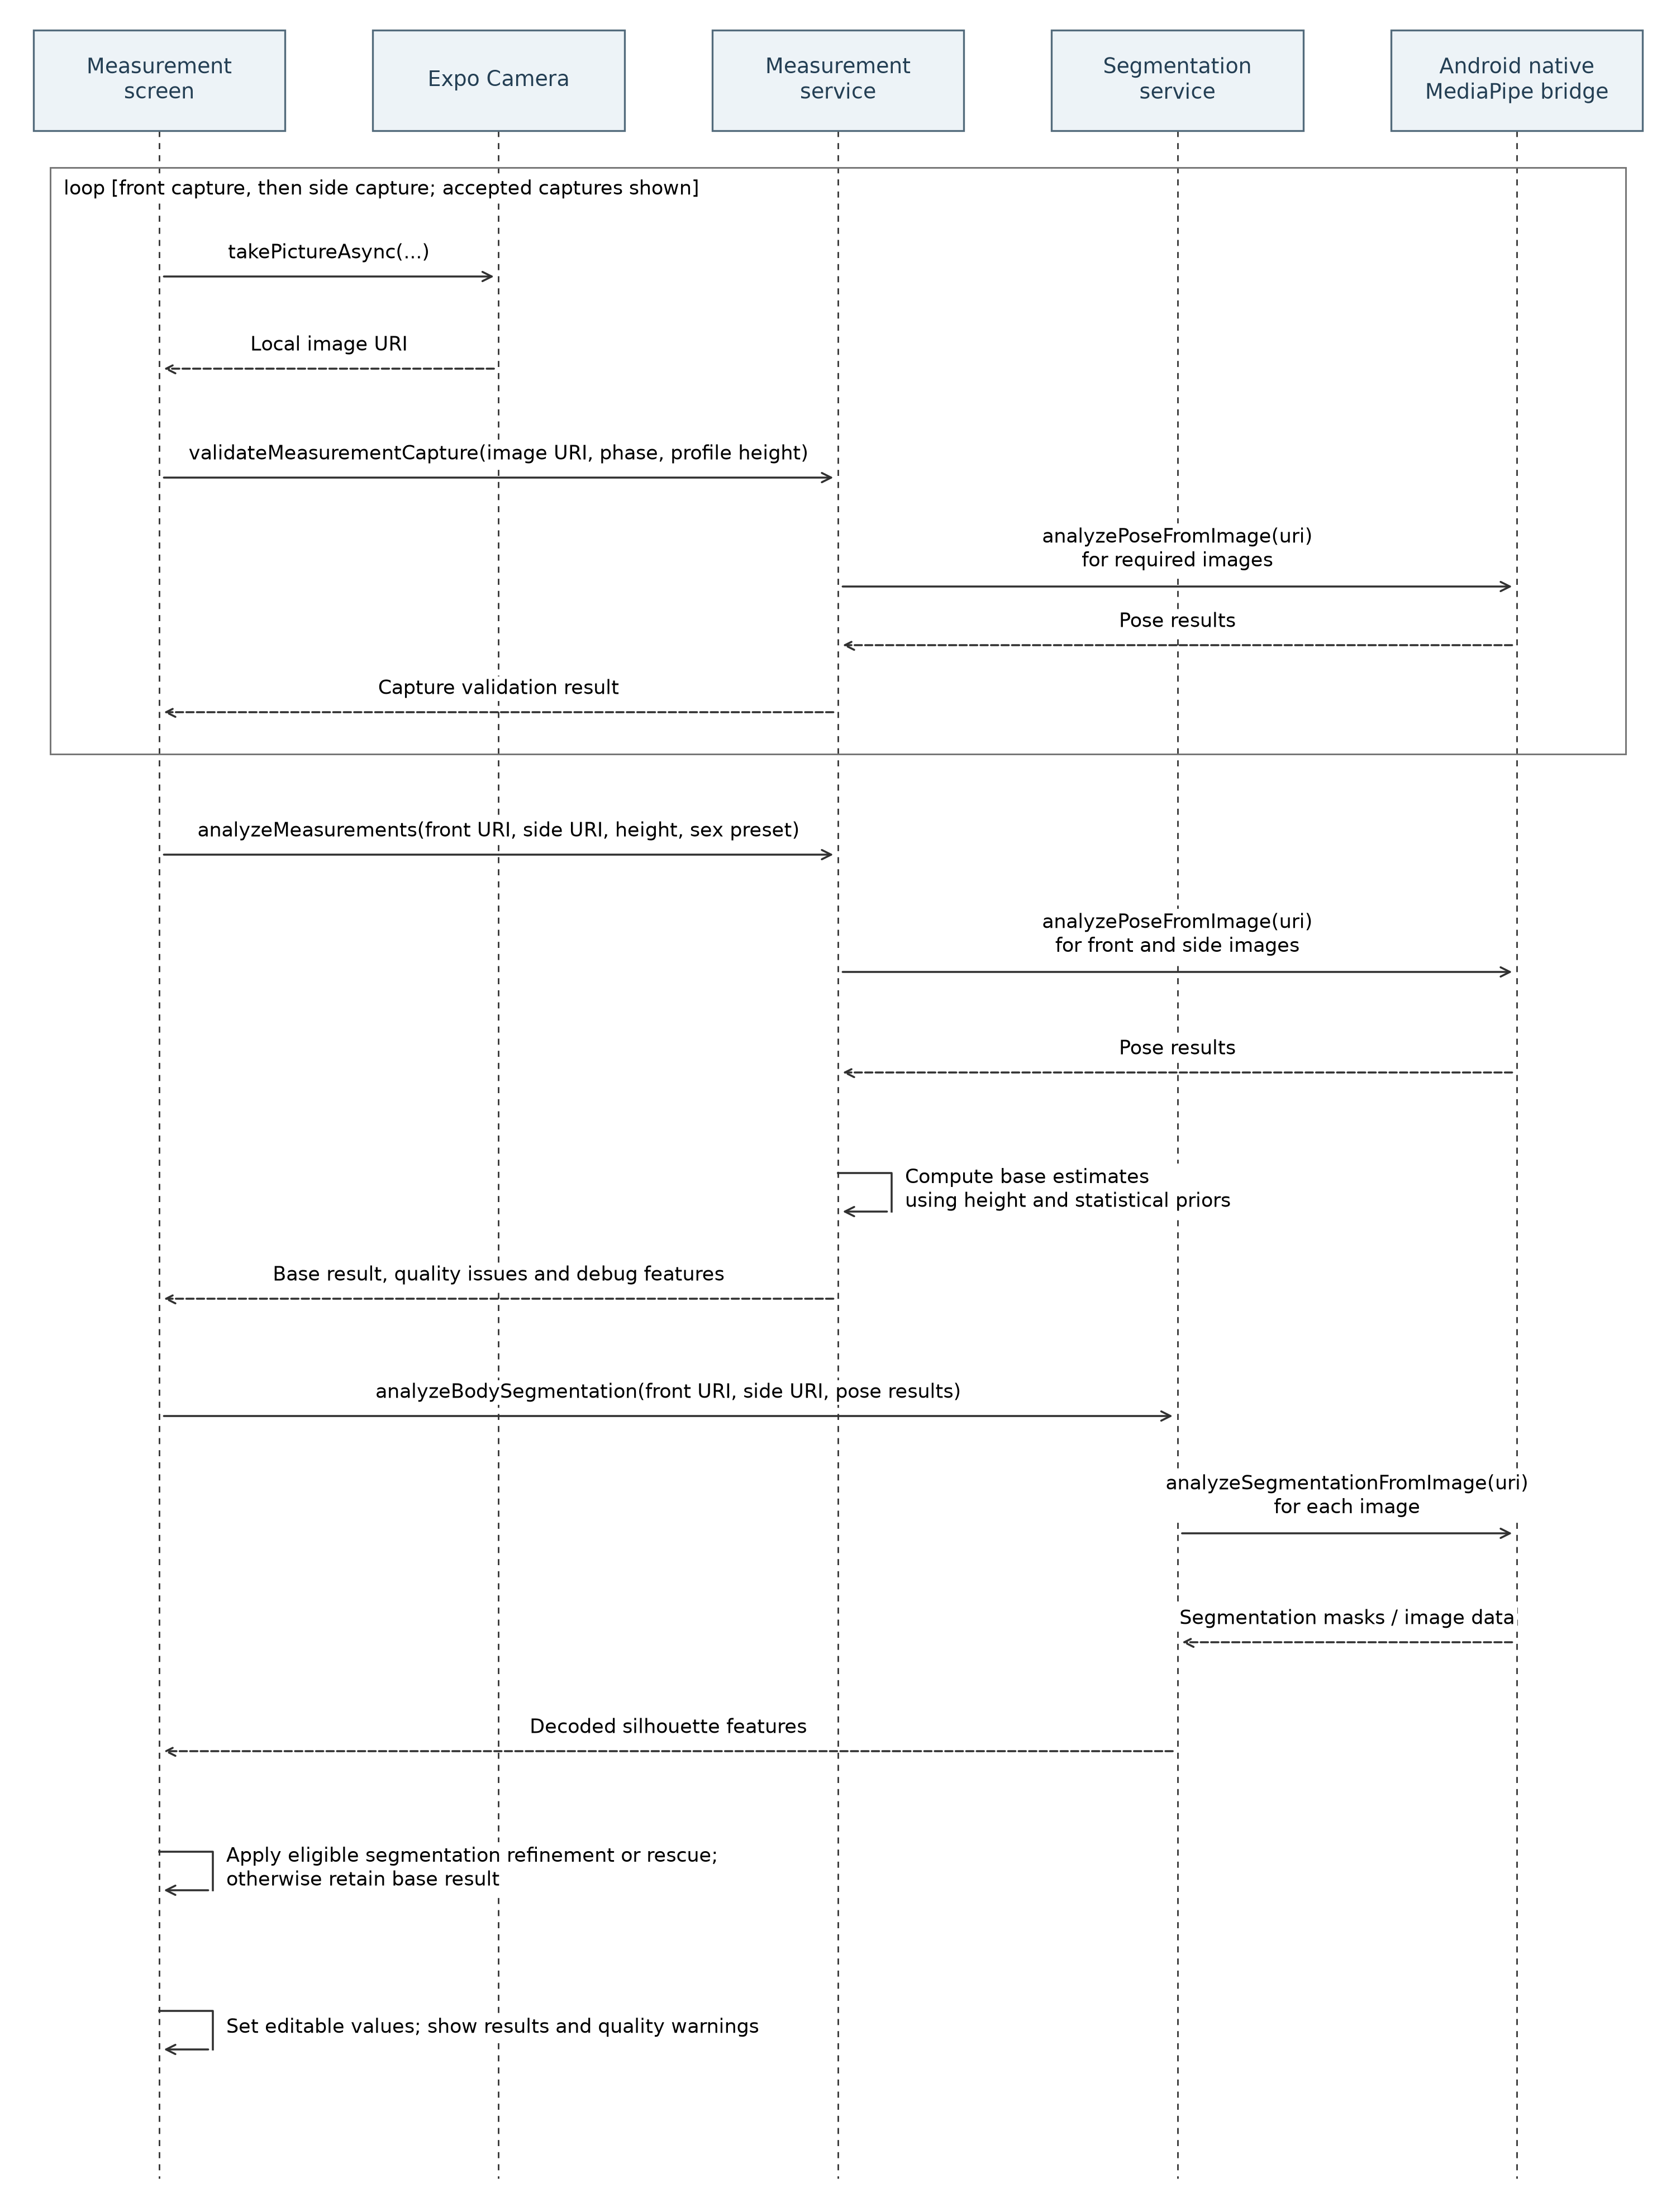
\includegraphics[width=0.92\linewidth]{figures/seq_measurement_detailed.png}
\caption{Technical sequence diagram: Selected Android body-measurement analysis path}
\label{fig:seq_measurement_detailed}
\end{figure}

Figure~\ref{fig:seq_measurement_ssd} makes the user journey explicit: introduction, front capture, side capture, editable results, and Save to progress. The selected path assumes accepted captures, passing save checks, an authenticated user, and successful remote persistence. Height is read from the profile rather than entered in the capture screen. The outputs are draft chest, waist, hip, and shoulder estimates, accompanied by capture-quality indicators. Their review and correction provide user control but do not demonstrate agreement with reference measurements.

Figure~\ref{fig:seq_measurement_detailed} selects the Android path in which MediaPipe pose and segmentation calls succeed. Expo Camera returns local image URIs. The measurement service validates the front capture before side capture; side validation also reuses the front image for comparison. Required images are analyzed individually through the Kotlin bridge's \texttt{analyzePoseFromImage(uri)} interface. The main estimation call analyzes the images again, converts pose features using profile height, and applies statistical depth priors selected using the profile's sex value or a neutral preset. The screen separately calls the segmentation service, which invokes \texttt{analyzeSegmentationFromImage(uri)} for each image. These calls can execute concurrently; the figure summarizes their per-image results rather than imposing an execution order. Screen-level functions then attempt segmentation-depth refinement, followed by a segmentation-based rescue when eligible, otherwise retaining the base result. Geometry and plausibility checks can still require a retake. The figure omits diagnostic comparison calls, local scan logging, and detailed numerical formulas.

This path is platform-dependent. Primary pose analysis attempts MediaPipe on Android and falls back to MoveNet on failure; other platforms select MoveNet directly, requiring a compatible native runtime. The supplied iOS MediaPipe bridge throws unimplemented errors for both pose and segmentation. Consequently, the Android sequence does not establish an equivalent MediaPipe pipeline or verified measurement behavior on iOS. Segmentation failure is caught by the screen and can leave the base estimate available for review, subject to the save checks.

\begin{figure}[H]
\centering
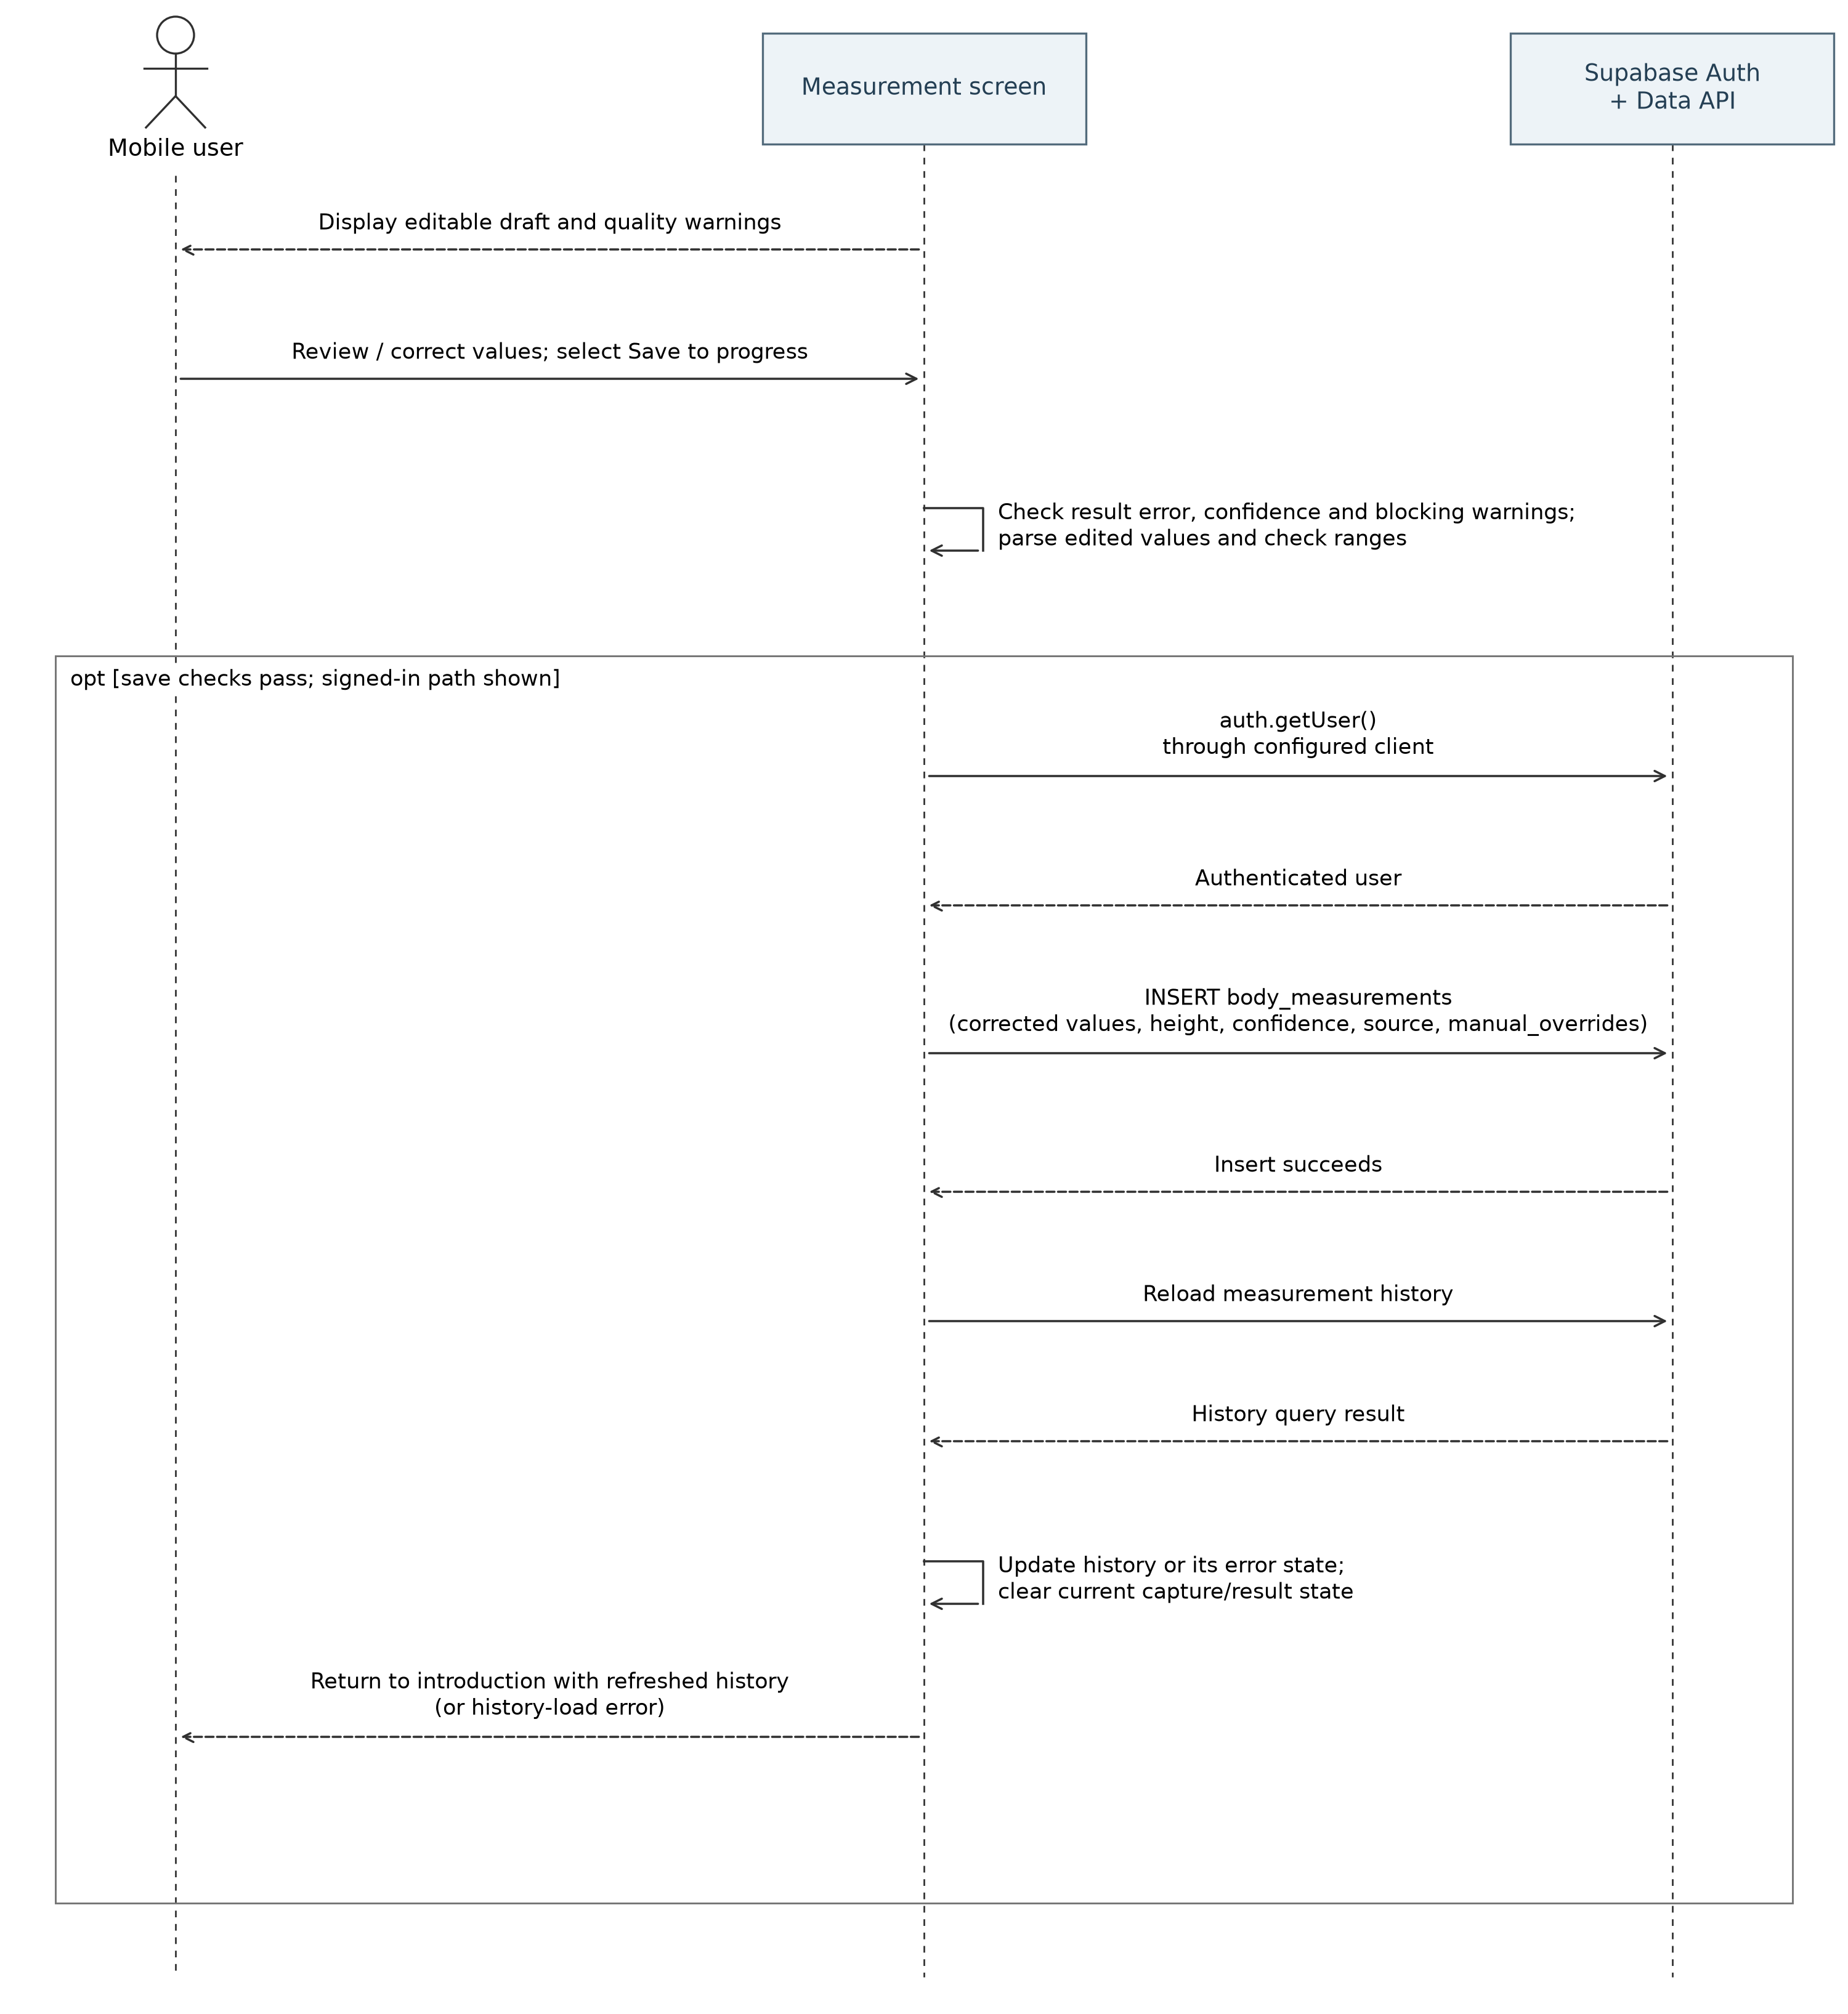
\includegraphics[width=0.95\linewidth]{figures/seq_measurement_save.png}
\caption{Technical sequence diagram: User review and successful body-measurement persistence}
\label{fig:seq_measurement_save}
\end{figure}

Figure~\ref{fig:seq_measurement_save} separates review and persistence from inference. The screen rejects result errors, confidence below the configured minimum of 0.25, blocking quality warnings, invalid edited values, or values outside its expected ranges. This threshold is an implementation gate, not an accuracy percentage. Displayed capture-quality indicators can also reflect anomaly penalties, while the inserted \texttt{measurement\_confidence} retains the result's original confidence value. After resolving the authenticated user through the configured Supabase client, the screen inserts corrected centimeter values into \texttt{body\_measurements}. The payload includes height, \texttt{source = ai\_ondevice}, original AI values, a feature vector when available, and corrected-field metadata within \texttt{manual\_overrides}. This save path uploads no photos and sets no \texttt{is\_verified} flag. It performs no application-level photo-encryption or Storage-upload step. Successful insertion is followed by a history reload and reset of capture/result state. History loading handles its own failures, so a saved measurement can coexist with a history-display error. No offline queue is implemented in this save handler; the remote save requires backend access. Local processing and model confidence alone do not establish anthropometric accuracy.


\subsubsection{Use case: Track daily nutrition and macro targets}

\begingroup
\footnotesize
\setlength{\tabcolsep}{3pt}
\renewcommand{\arraystretch}{1.20}
\setlength{\LTpre}{5pt}
\setlength{\LTpost}{10pt}
\begin{longtable}{|L{4.95cm}|L{10.05cm}|}
\caption{Textual description of use case: Track daily nutrition and macro targets}\label{tab:pdf-52-24} \\
\hline
\rowcolor{entetetab}
Field & Description \\ \hline
\endfirsthead
\hline
\rowcolor{entetetab}
Field & Description \\ \hline
\endhead
Use case & Track daily nutrition and macro targets \\ \hline
Primary actor & Mobile user \\ \hline
Preconditions & The user is authenticated and backend access is available. Barcode scanning requires camera permission. Nutrition goals may already exist or be initialized with defaults; dietary preferences are optional. \\ \hline
Postconditions & On successful insertion, a \texttt{meal\_logs} record references a food item, serving quantity, meal type, date, and user. A subsequent successful refresh updates shared logs, totals, and weekly-summary state used by the Nutrition screen. A refresh failure can leave a saved record with stale displayed totals. \\ \hline
Nominal scenario & 1. The user opens Nutrition and selects Add Food. 2. The user searches the catalog by name or opens the barcode scanner. 3. For a barcode, the service first queries the remote food catalog; a miss invokes a lookup Edge Function, which rechecks the catalog and, if necessary, requests product data from Open Food Facts. 4. A matching product is selected and its serving basis is displayed. 5. The user enters a serving multiplier, selects the meal type, and confirms logging for the selected date. 6. The application inserts the meal log, attempts a nutrition-data refresh, and returns to Nutrition, where successful refreshed totals are displayed against goals. \\ \hline
Alternative scenario & 2.1. Name search excludes food names containing declared allergy or dislike terms; this is not ingredient-based allergen verification. 5.1. The user can log recent foods or reusable saved meals. Separate nutrition actions support saving meal combinations and logging water with +250ml or +500ml buttons. \\ \hline
Exception scenario & E.1. Missing barcode matches or lookup failures display a message inviting manual catalog search. E.2. Denied camera permission prevents opening the scanner and displays a permission message. E.3. Failed text search clears the results; no device-cache fallback is implemented in this search path. E.4. Invalid serving input prevents submission. Authentication or insertion failures reject the logging operation; refresh failures are recorded in shared error state after any successful insertion. \\ \hline
\end{longtable}
\endgroup

\begin{figure}[H]
\centering
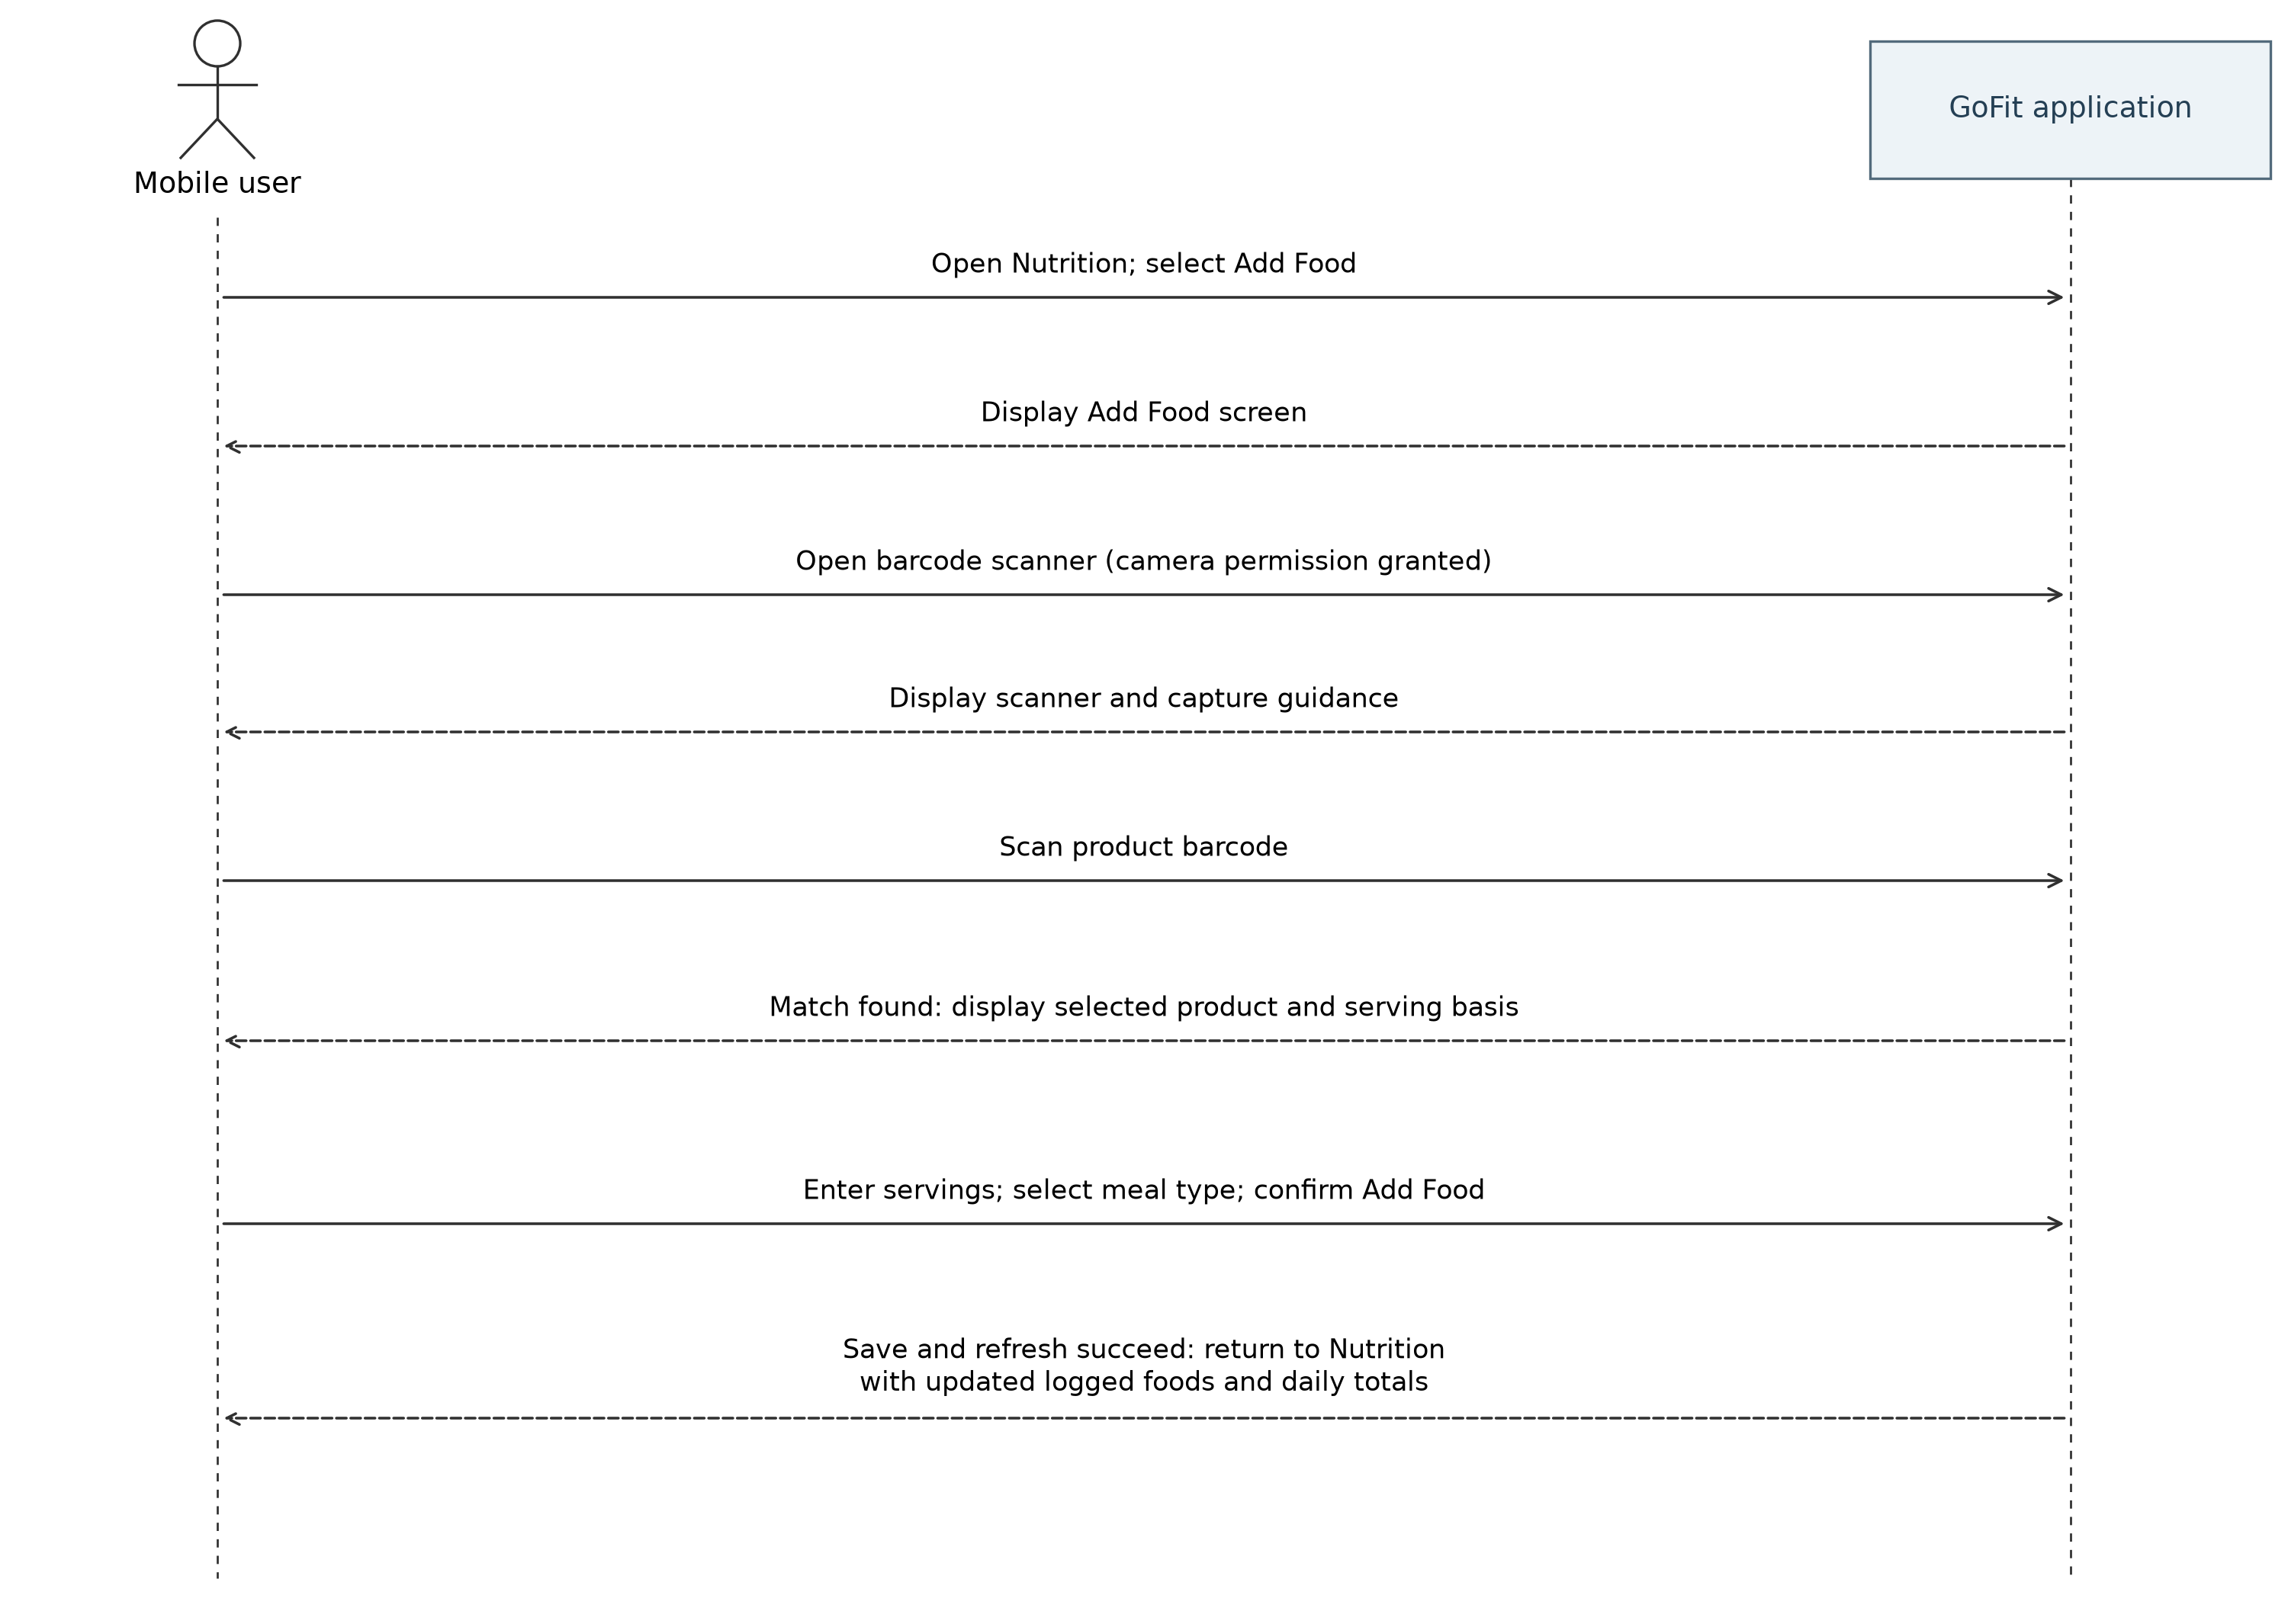
\includegraphics[width=0.92\linewidth]{figures/seq_nutrition_ssd.png}
\caption{System sequence diagram: Barcode selection and successful meal logging}
\label{fig:seq_nutrition_ssd}
\end{figure}

\begin{figure}[H]
\centering
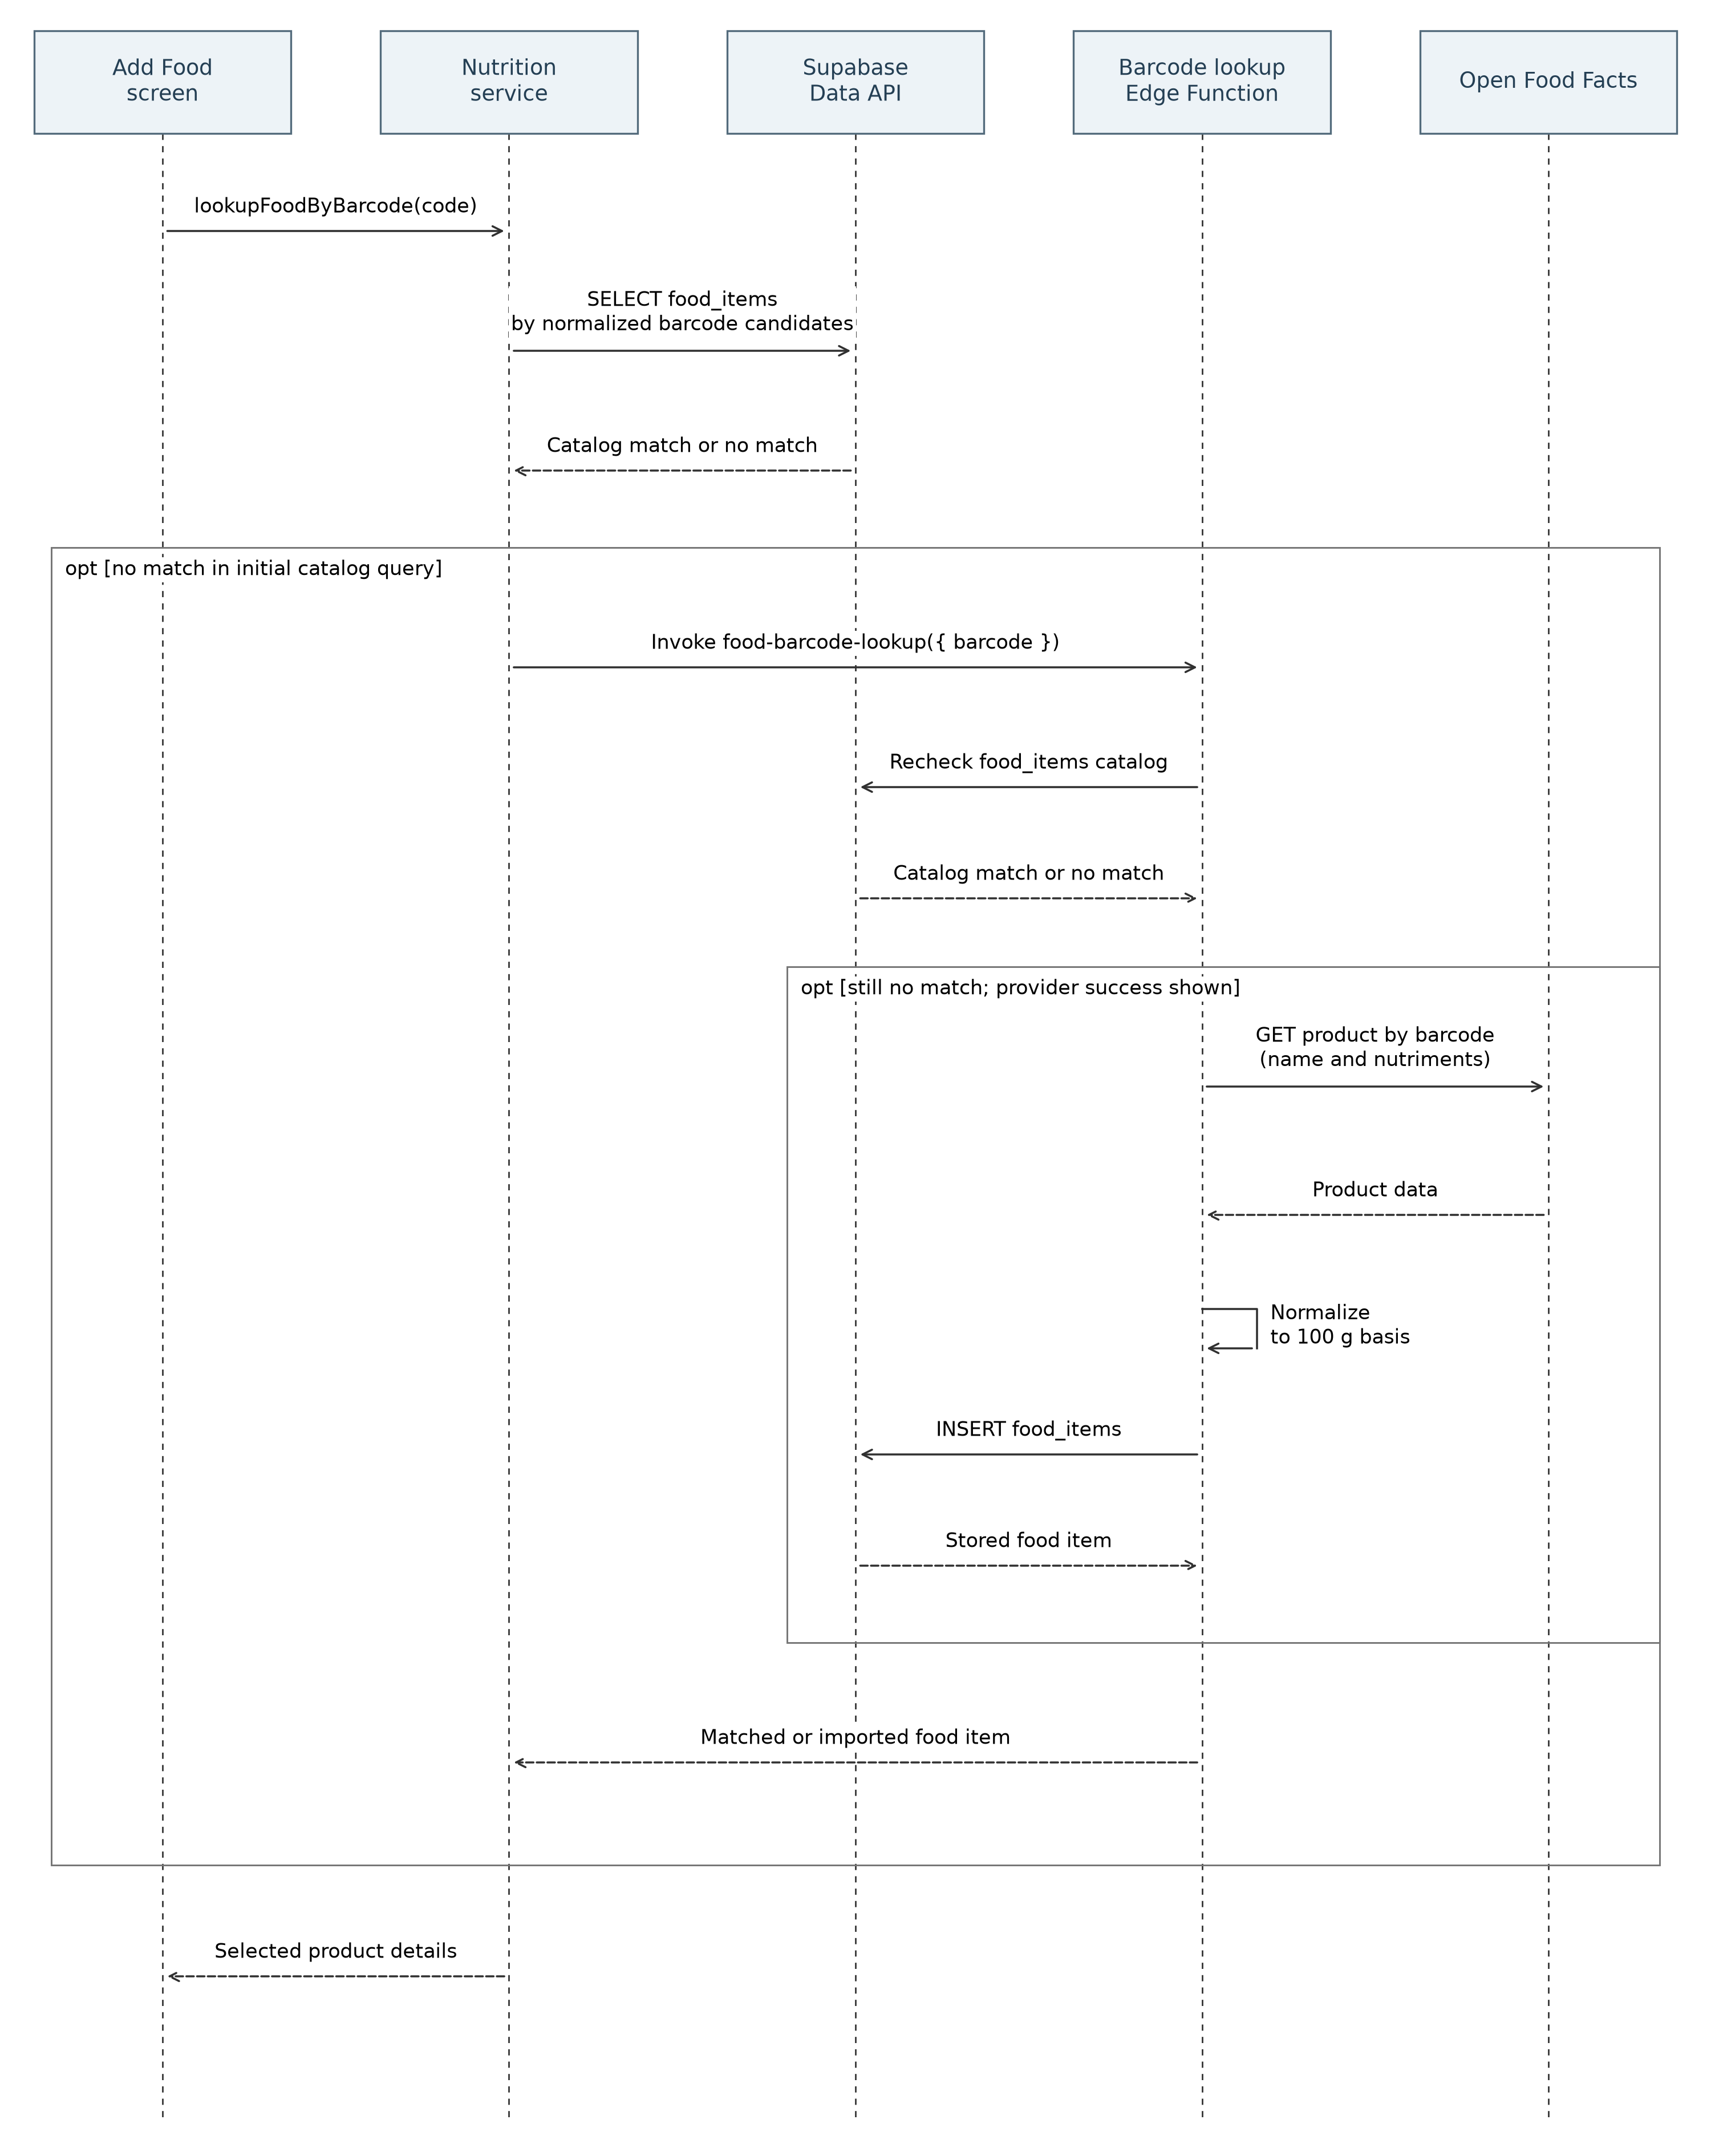
\includegraphics[width=0.92\linewidth]{figures/seq_nutrition_detailed.png}
\caption{Technical sequence diagram: Catalog-first barcode lookup and provider fallback}
\label{fig:seq_nutrition_detailed}
\end{figure}

Figure~\ref{fig:seq_nutrition_ssd} shows the successful barcode journey through Nutrition, Add Food, the camera scanner, product selection, and meal logging. The user enters a serving multiplier rather than an independently interpreted gram quantity. Food details include the catalog serving label; products imported by the lookup function use a 100 g basis, so 1.5 servings represents 150 g for those products. Submission accepts finite quantities greater than zero and no greater than 50 servings. Product and lookup failures do not follow the successful continuation shown.

Figure~\ref{fig:seq_nutrition_detailed} separates lookup responsibilities. AddFoodScreen calls the nutrition service directly. The initial catalog query reads \texttt{food\_items} through the Supabase Data API, normalizing barcode candidates to accommodate supported leading-zero variants. This catalog is remote, not an offline device cache. A miss invokes \texttt{food-barcode-lookup}; the function rechecks the same catalog and only contacts Open Food Facts if no match exists. For a usable provider response, it normalizes product names and nutrients to its 100 g serving basis, inserts a food item, and returns that item. The figure selects the provider-success path; invalid codes, provider failures, missing or unusable products, and the insertion-race recovery branch are omitted. The function includes a re-query after insertion failure to recover a concurrently inserted matching item. These source artifacts establish implementation, not a successful deployed lookup test.

Name-search exclusions belong to a separate interaction. AddFoodScreen collects allergy and dislike terms from the profile and passes them to \texttt{searchFoods}; the service applies case-insensitive name matching and negated name matches to the remote catalog query. The barcode path does not perform ingredient-conflict analysis, and the provider request retrieves names and nutrient data rather than an ingredient/allergen evaluation. Neither name exclusion nor a barcode match establishes that a product is safe for a declared allergy. When lookup fails or no product is found, the interface invites manual catalog search, not direct entry of arbitrary nutrient values.

\begin{figure}[H]
\centering
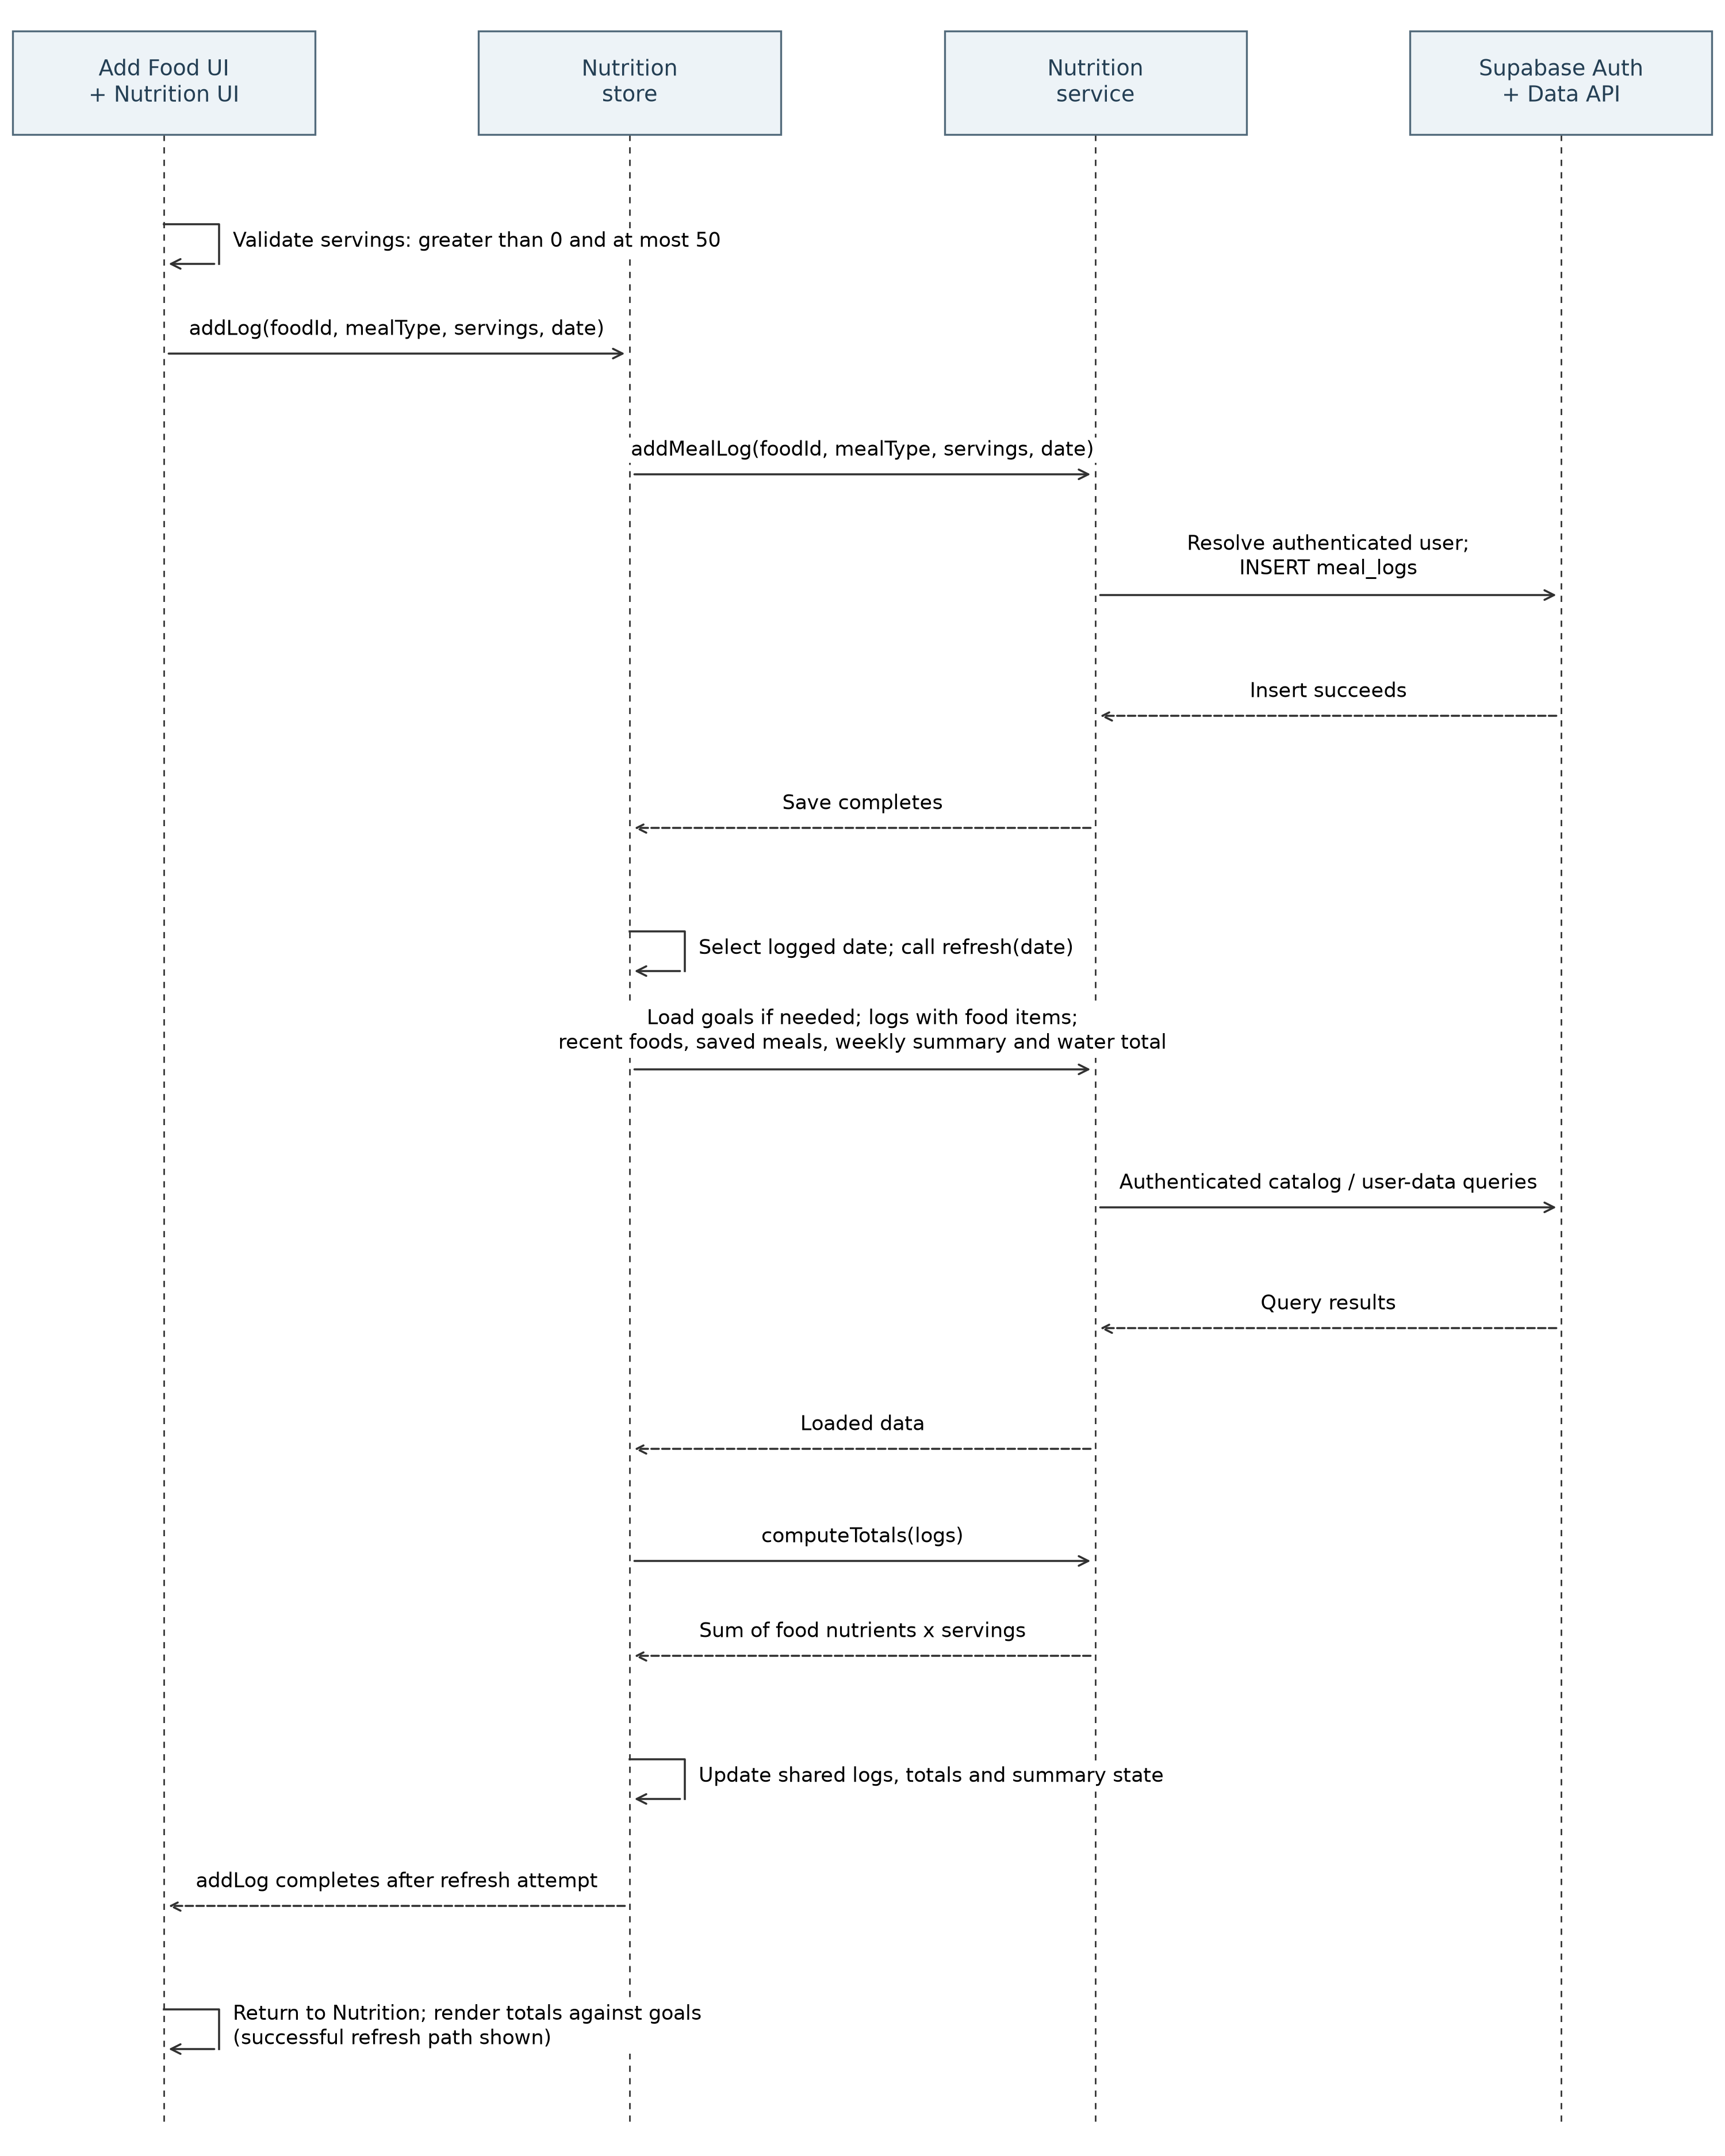
\includegraphics[width=0.95\linewidth]{figures/seq_nutrition_logging.png}
\caption{Technical sequence diagram: Meal-log insertion and successful nutrition refresh}
\label{fig:seq_nutrition_logging}
\end{figure}

Figure~\ref{fig:seq_nutrition_logging} shows AddFoodScreen delegating persistence to the nutrition store and service. The service resolves the authenticated user and inserts \texttt{user\_id}, \texttt{food\_item\_id}, \texttt{meal\_type}, \texttt{servings}, and \texttt{logged\_date} into \texttt{meal\_logs}. Nutrient values remain associated with the referenced food item. The store then selects the logged date and invokes its refresh routine, which loads goals if needed, meal logs joined to foods, recent foods, saved meals, a weekly summary, and water totals. The figure groups these service queries for readability rather than expanding their exact interleaving; the totals computation is shown separately to identify its owner. \texttt{nutritionService.computeTotals(logs)} sums each food's nutrient values multiplied by its logged servings. Water is added from its separate log total, and the store updates the state consumed by MacroRings and other nutrition views. AddFoodScreen returns to Nutrition after the logging action completes; screen focus also triggers a refresh. The two screens share an explicitly grouped UI participant in the figure. This is request-based refresh behavior rather than evidence of a realtime subscription. A successful insert can be followed by a caught refresh failure, leaving an error and stale display state even though navigation returns to Nutrition. Default goals are implementation defaults and do not imply individually assessed nutritional targets.


\section{Realisation}

The exercise library provides faceted search across muscle groups, difficulty tiers, and equipment categories, with video stream integration hosted on Cloudflare R2.


Progress dashboards feature interactive Victory Native charts rendering bodyweight velocity, cumulative volume, 1RM strength curves, and side-by-side progress photo comparisons.


The nutrition module features animated MacroRings displaying real-time caloric, protein, carbohydrate, and fat budgets, paired with camera barcode scanning via OpenFoodFacts.


The AI body measurement pipeline runs on-device using MediaPipe BlazePose (33 3D landmarks) and Selfie Segmentation to compute waist, chest, and hip metrics calibrated against user height.


\subsection{Progress, Nutrition, and Reminder Features}

Sprint 2 connected the workout foundation to user progress. A fitness application becomes more valuable when it transforms repeated sessions into understandable feedback. For this reason, the sprint added progress screens, history views, statistics, body-measurement foundations, nutrition-related flows, and reminder infrastructure. These features help users move from isolated workout execution to long-term self-monitoring.


Progress tracking uses workout session data, body-measurement data, and optional nutrition entries to display user evolution. Empty states are important in this sprint because new users may not have enough data yet. The interface should explain what the user can do next without showing broken charts or misleading statistics.


\begingroup
\footnotesize
\setlength{\tabcolsep}{3pt}
\renewcommand{\arraystretch}{1.20}
\setlength{\LTpre}{5pt}
\setlength{\LTpost}{10pt}
\begin{longtable}{|L{3.67cm}|L{5.29cm}|L{5.73cm}|}
\caption{Sprint 2 user-facing progress modules}\label{tab:pdf-56-25} \\
\hline
\rowcolor{entetetab}
Module & Objective & Important states \\ \hline
\endfirsthead
\hline
\rowcolor{entetetab}
Module & Objective & Important states \\ \hline
\endhead
Exercise library & Allow users to browse and understand available exercises. & Search result, filter result, detail screen, no-result state, loading state. \\ \hline
Workout calendar/history & Help users see planned and completed training. & Scheduled workout, completed workout, missed day, empty calendar, history detail. \\ \hline
Progress dashboard & Summarize evolution over time. & Charts with data, first-use empty state, metric selector, date-range filtering. \\ \hline
Body measurements & Record and compare physical changes. & Manual entry, AI draft, review/correction, quality warning, saved measurement. \\ \hline
Nutrition/saved meals & Support nutrition tracking foundations. & Saved meal list, meal detail, item edit, history, reusable entry. \\ \hline
Notifications & Encourage consistency and communication. & Permission request, reminder settings, notification inbox, push-token registration. \\ \hline
\end{longtable}
\endgroup

Figure~\ref{fig:ui-progress-nutrition} combines the visible progress-chart state with nutrition and serving-entry views. The shown zero values and meal-entry form are interface observations; a completed save and aggregate correctness require the associated QA/readback records.

\begin{figure}[H]
\centering
\begin{minipage}[t]{.29\linewidth}
\centering
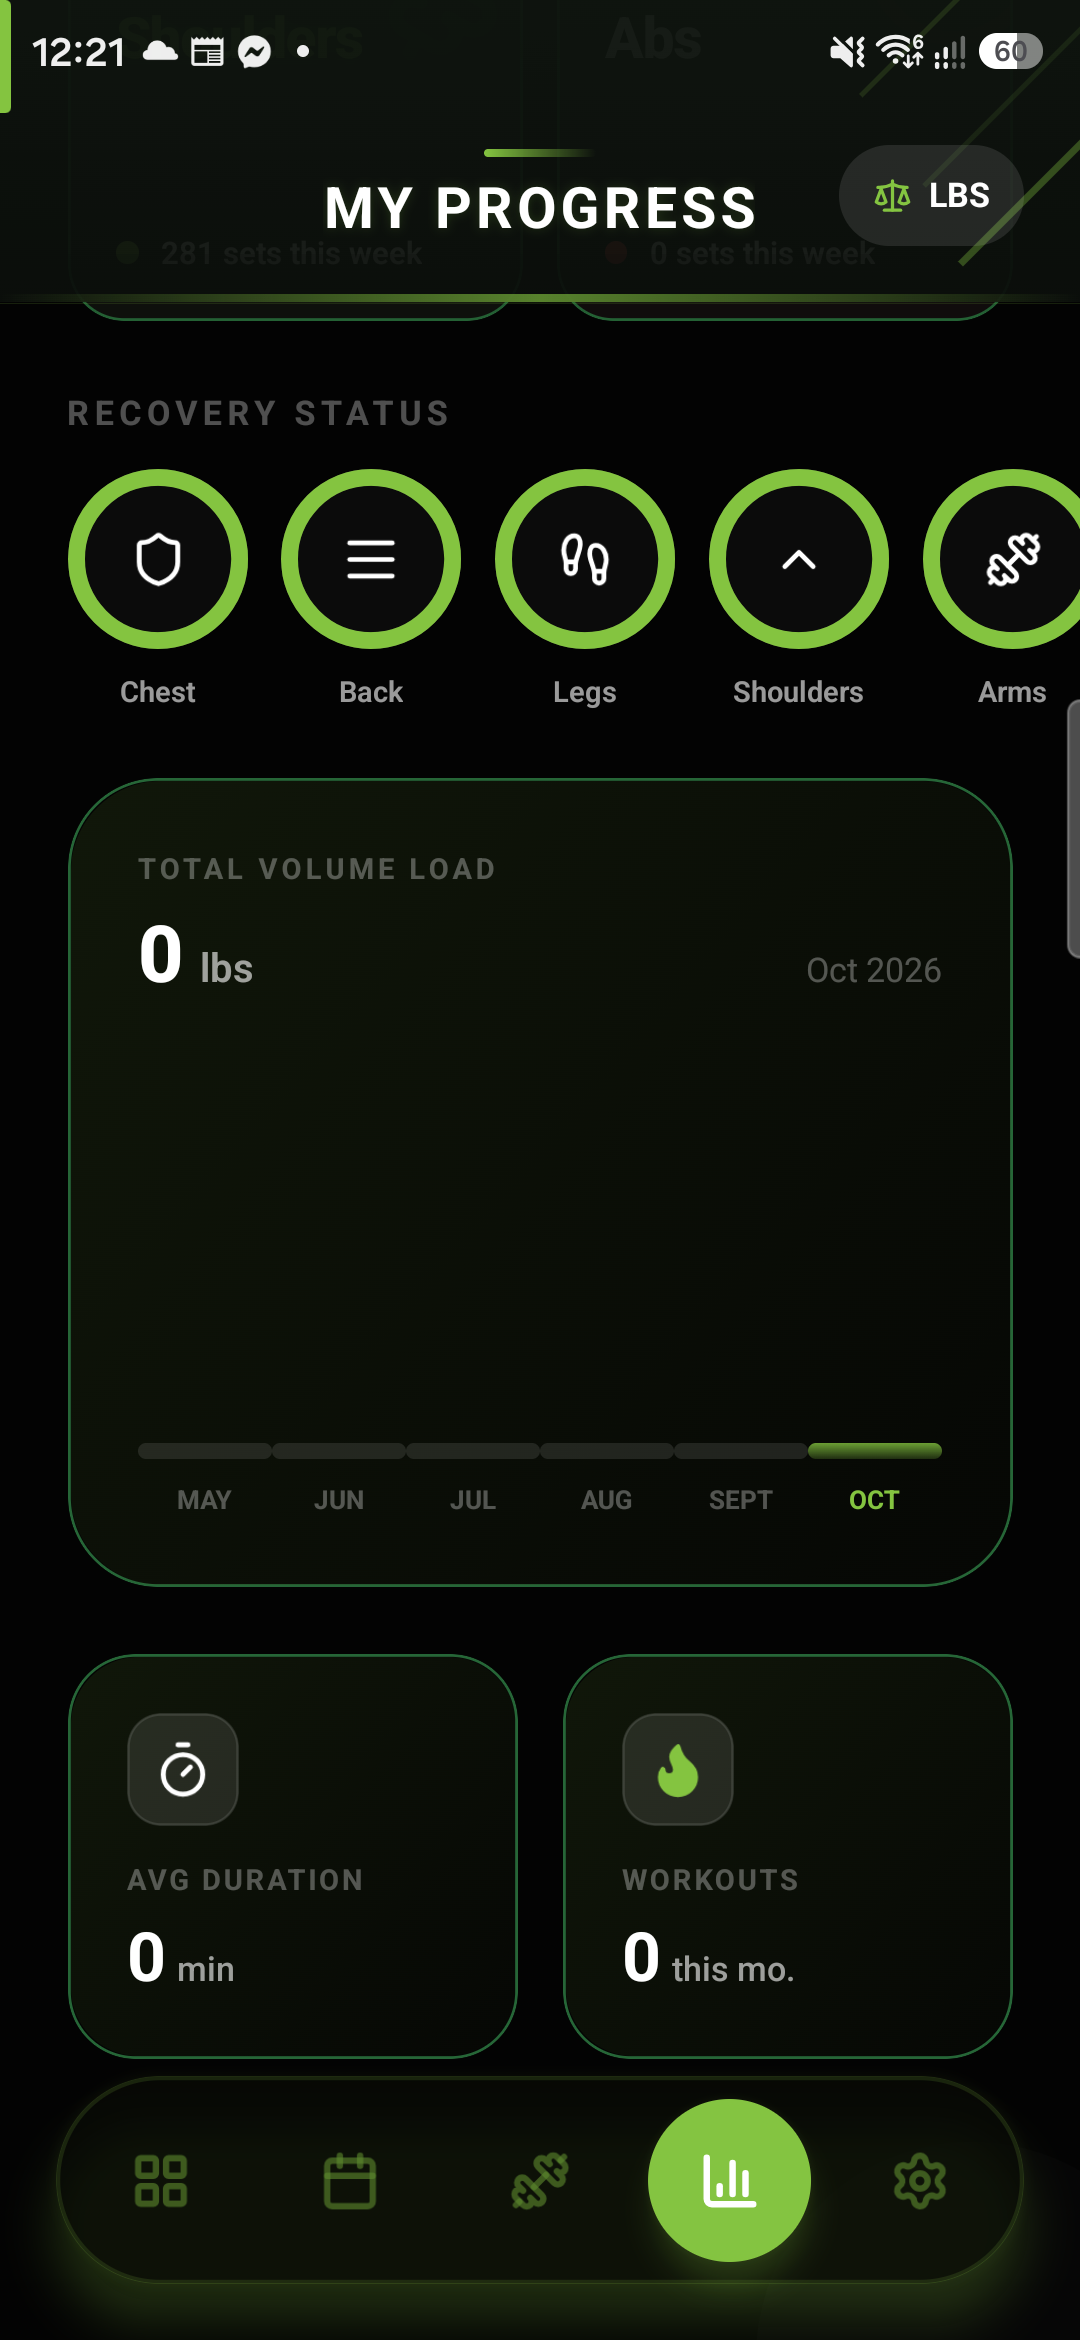
\includegraphics[width=\linewidth]{figures/screenshots/client-progress-chart.png}
\par\smallskip{\footnotesize a) Progress chart state\par}
\end{minipage}
\hspace{0.025\linewidth}
\begin{minipage}[t]{.29\linewidth}
\centering
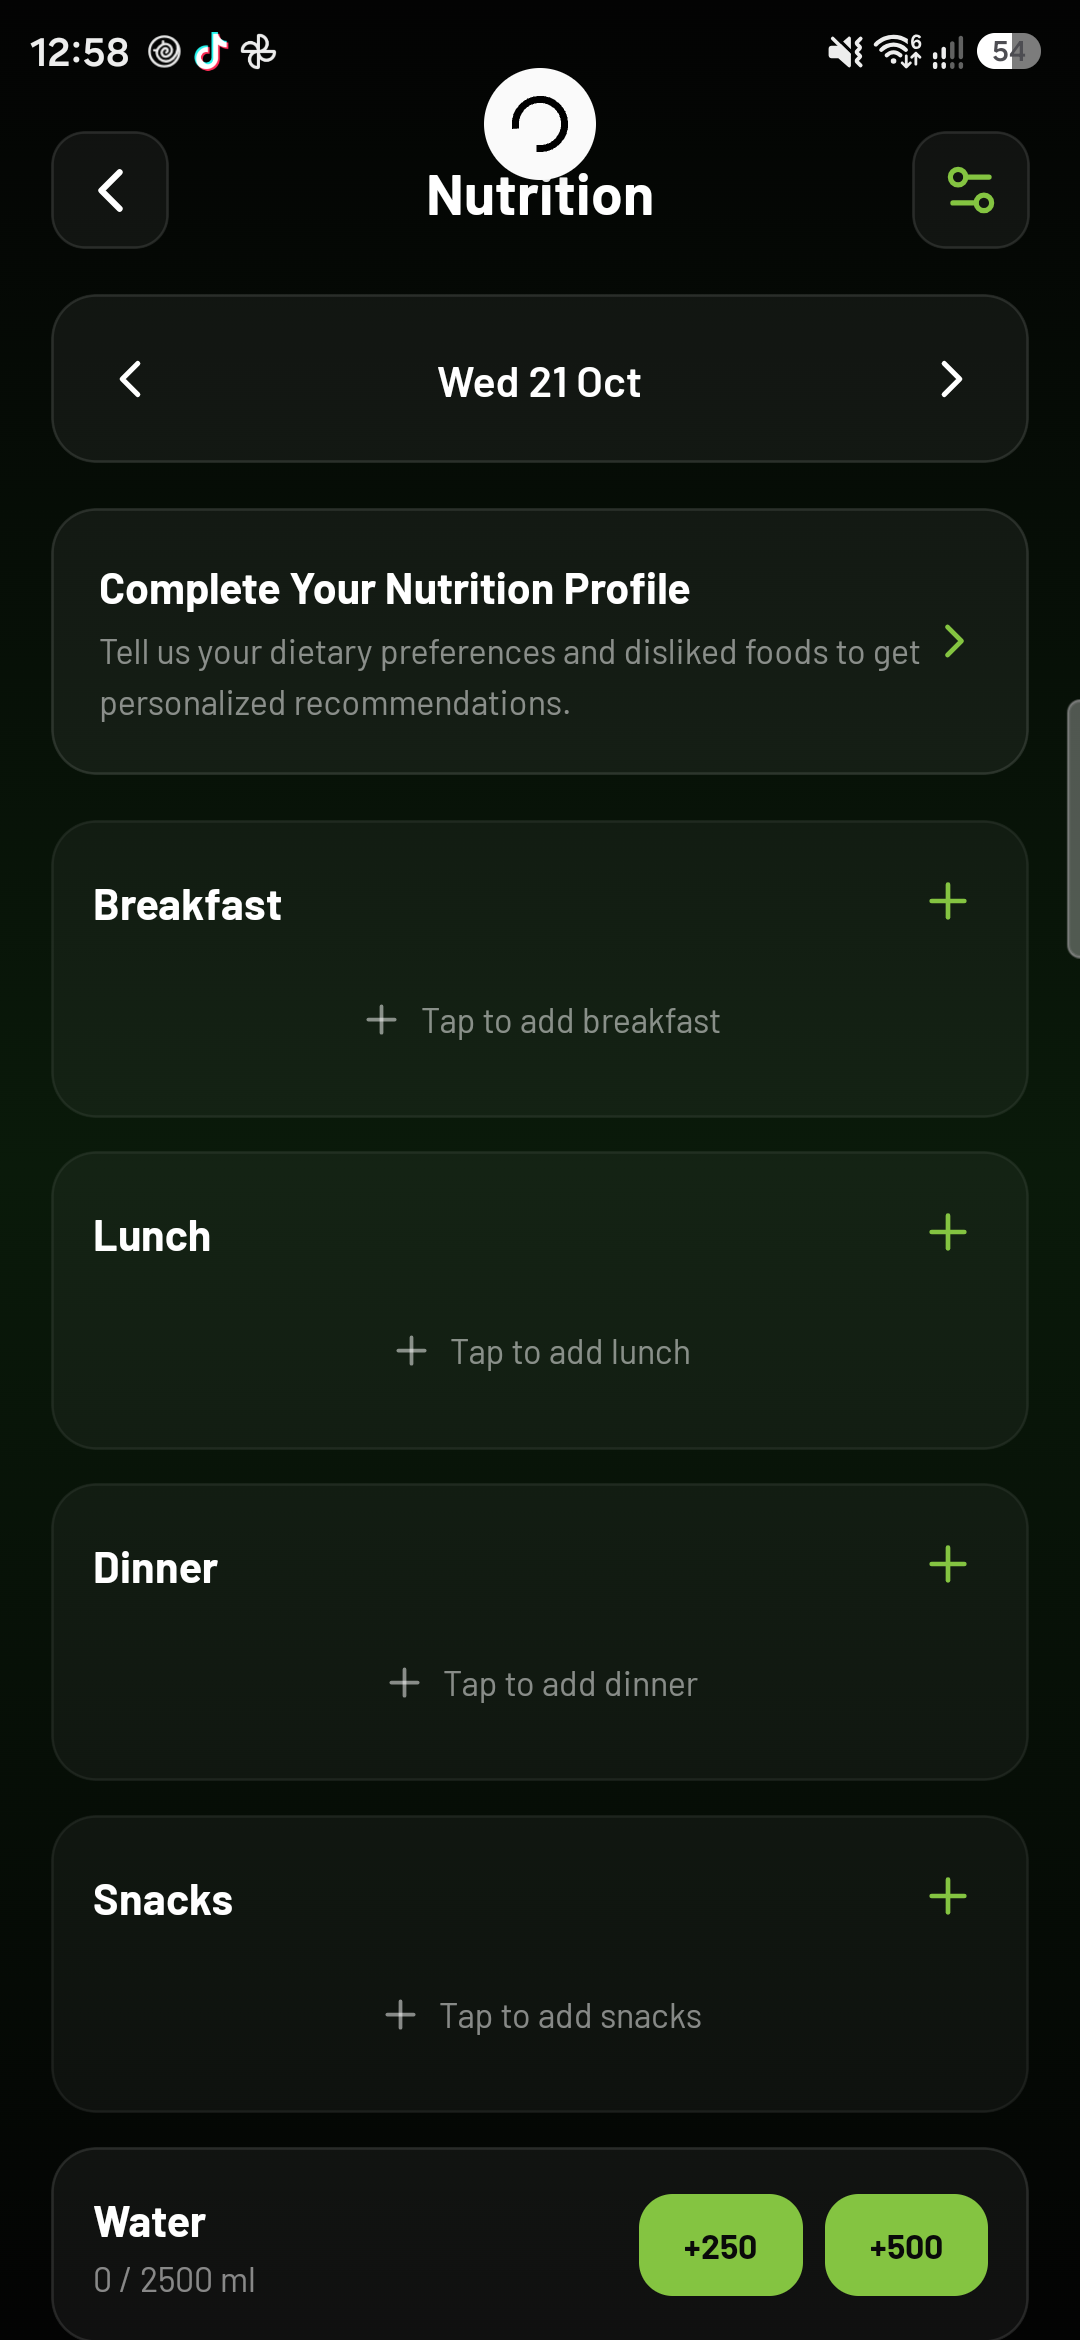
\includegraphics[width=\linewidth]{figures/screenshots/client-nutrition-dashboard.png}
\par\smallskip{\footnotesize b) Nutrition diary\par}
\end{minipage}
\hspace{0.025\linewidth}
\begin{minipage}[t]{.29\linewidth}
\centering
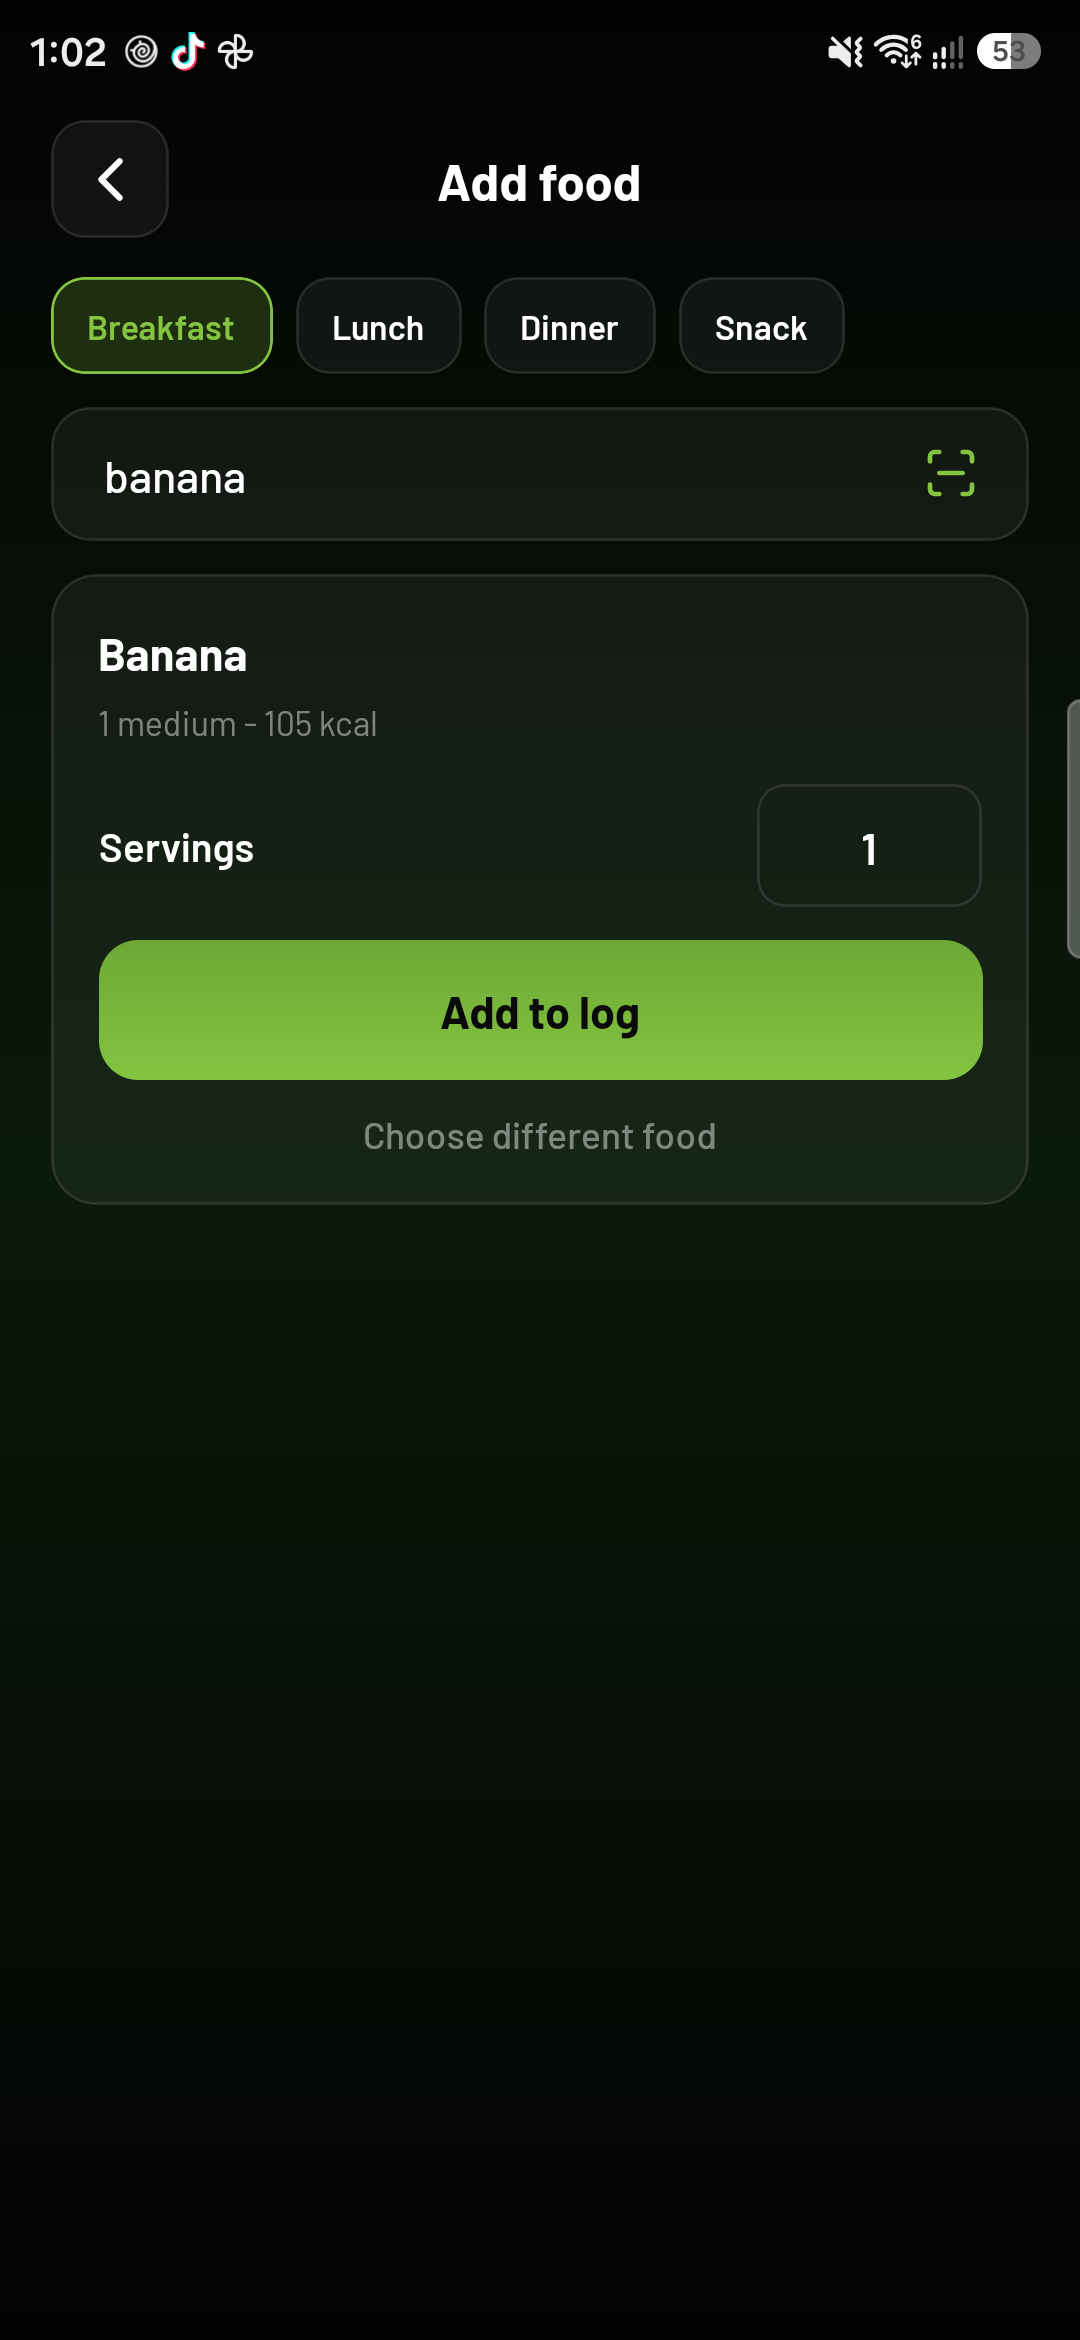
\includegraphics[width=\linewidth]{figures/screenshots/client-food-serving.png}
\par\smallskip{\footnotesize c) Selected food and serving\par}
\end{minipage}
\caption{Interface captures: progress display, nutrition diary and food-serving selection (October QA).}
\label{fig:ui-progress-nutrition}
\end{figure}

Figure~\ref{fig:ui-nutrition-extended} shows the goal form and the disposable food/saved-meal records from the retained QA. The goal values are displayed preferences rather than individualized dietary advice; saved-meal visibility does not establish every reuse/edit path.

\begin{figure}[H]
\centering
\begin{minipage}[t]{.29\linewidth}
\centering
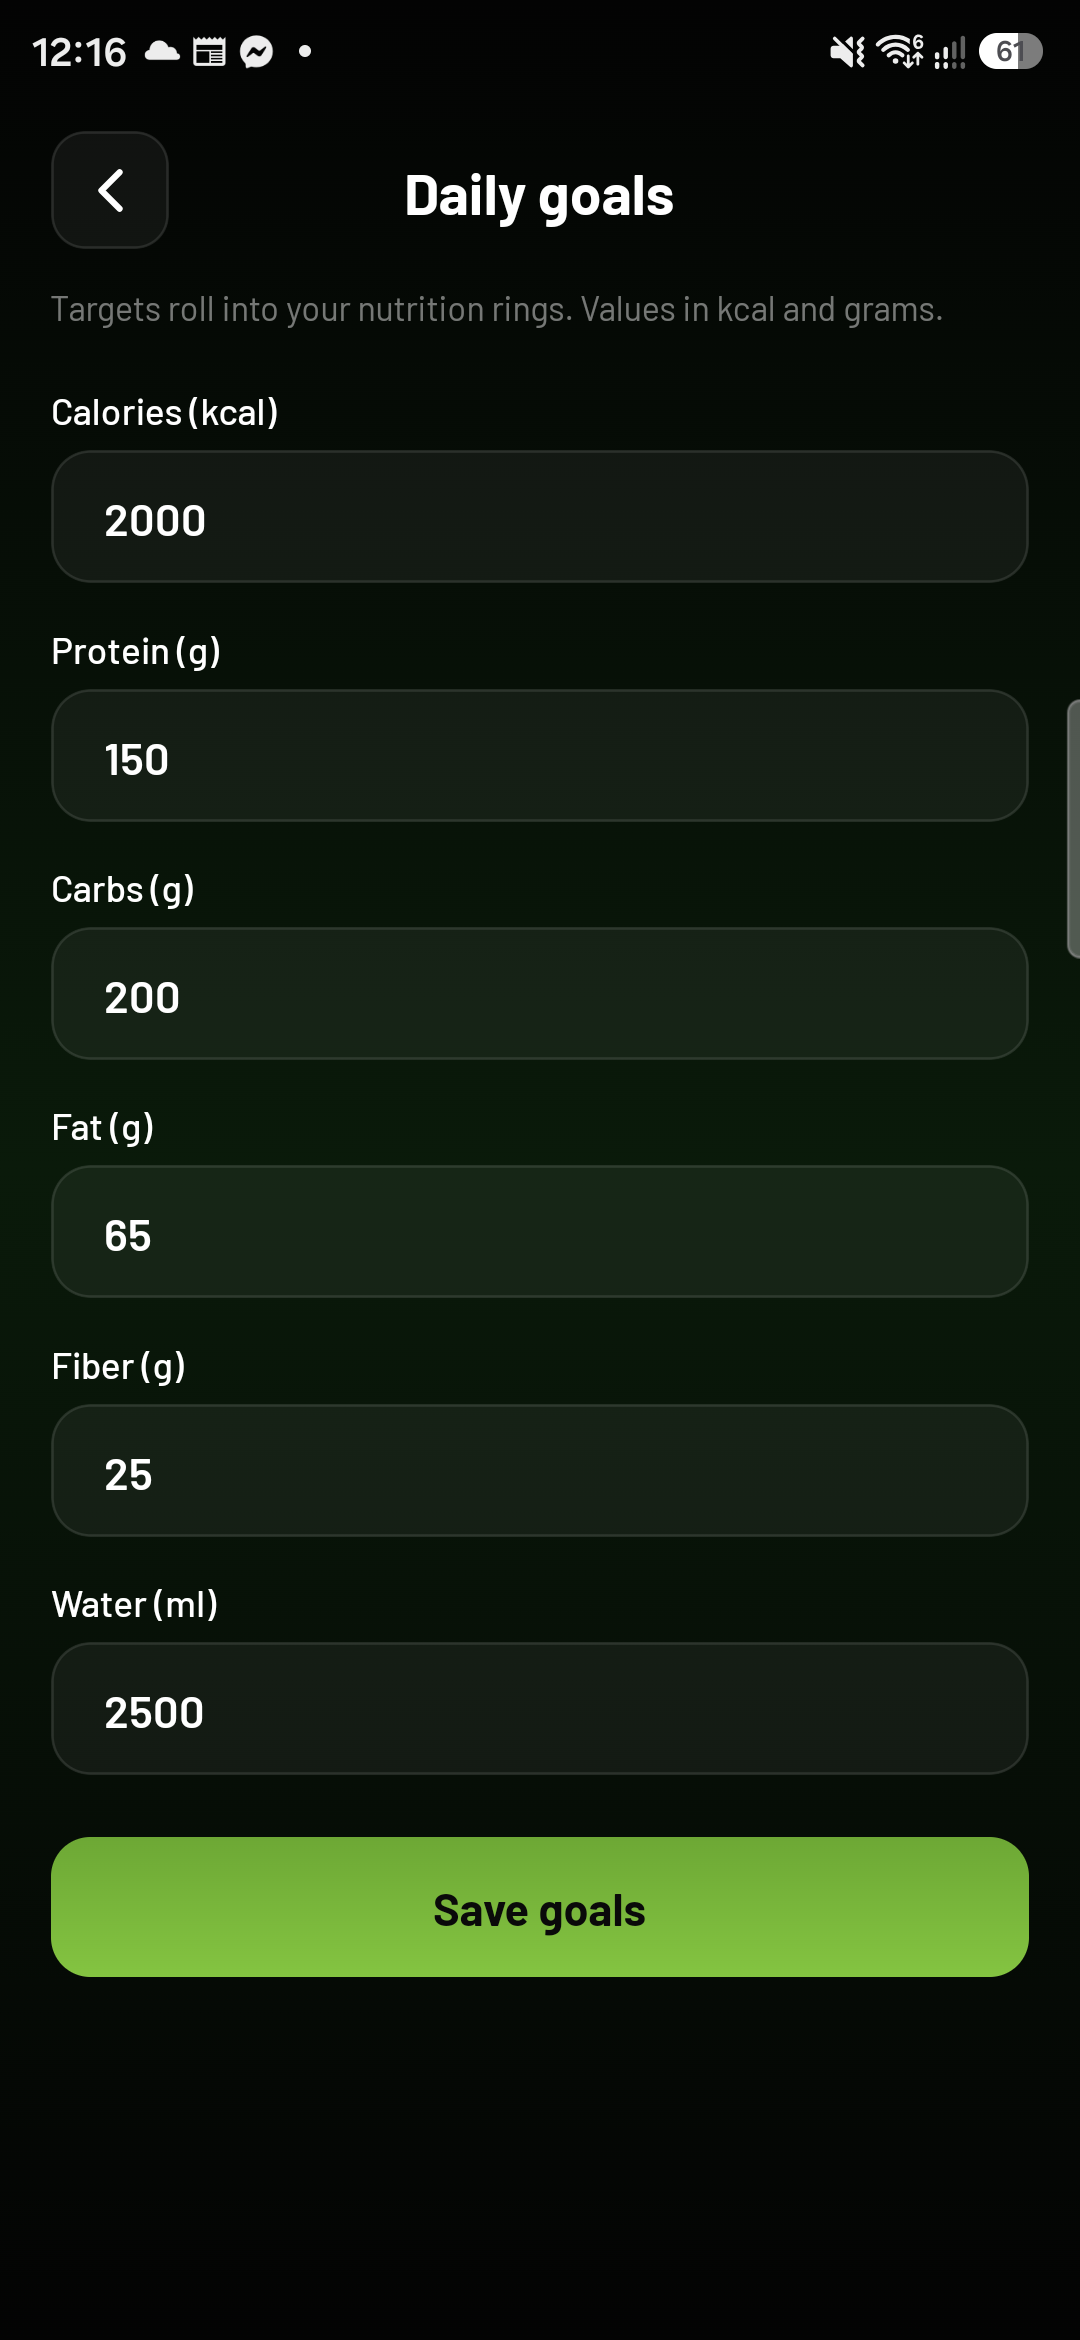
\includegraphics[width=\linewidth]{figures/screenshots/client-nutrition-goals.png}
\par\smallskip{\footnotesize a) Displayed daily targets\par}
\end{minipage}
\hspace{0.025\linewidth}
\begin{minipage}[t]{.29\linewidth}
\centering
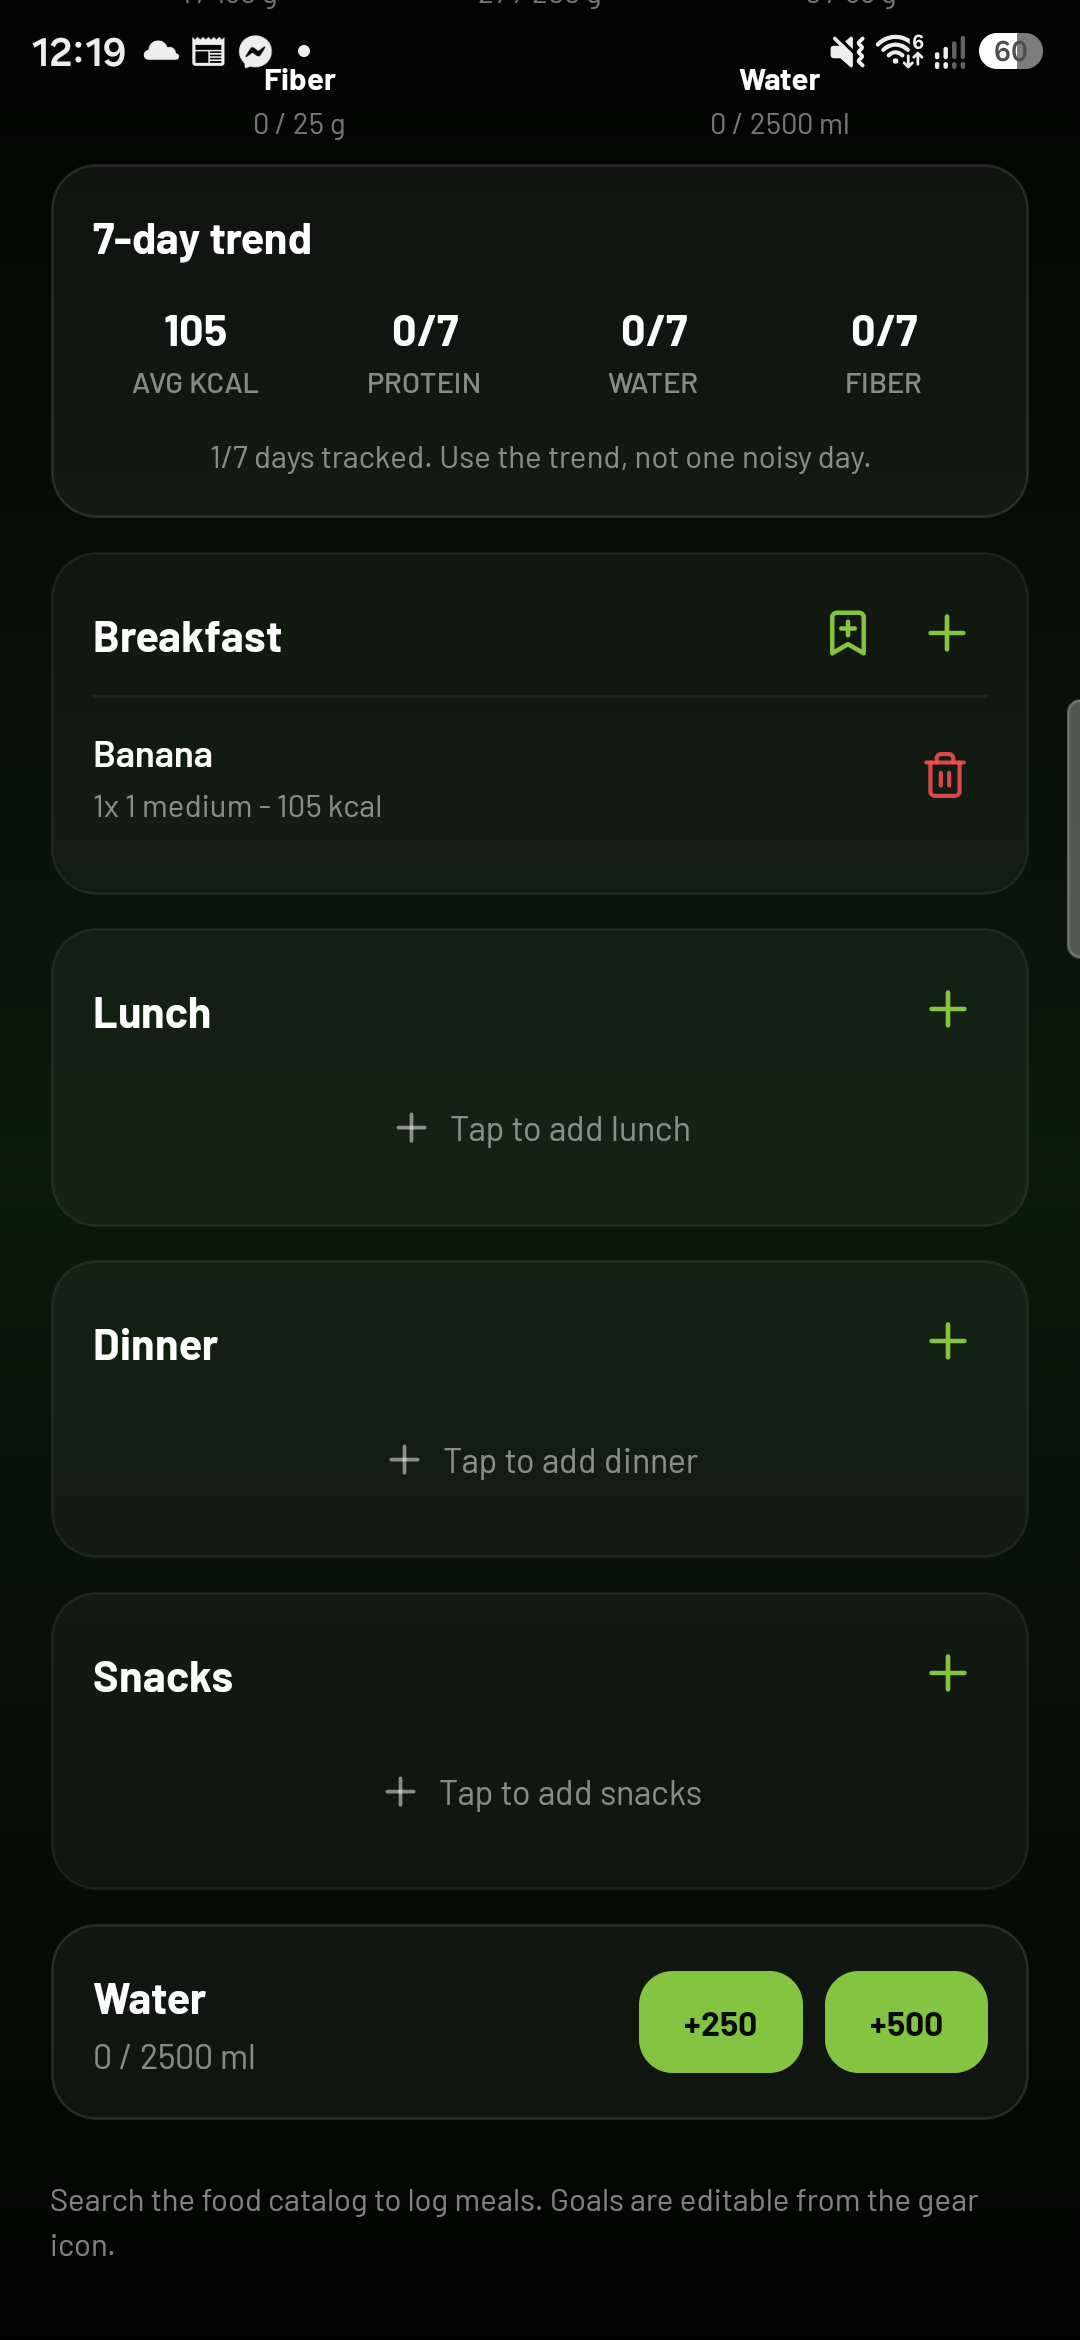
\includegraphics[width=\linewidth]{figures/screenshots/client-disposable-food-log.png}
\par\smallskip{\footnotesize b) Disposable banana log\par}
\end{minipage}
\hspace{0.025\linewidth}
\begin{minipage}[t]{.29\linewidth}
\centering
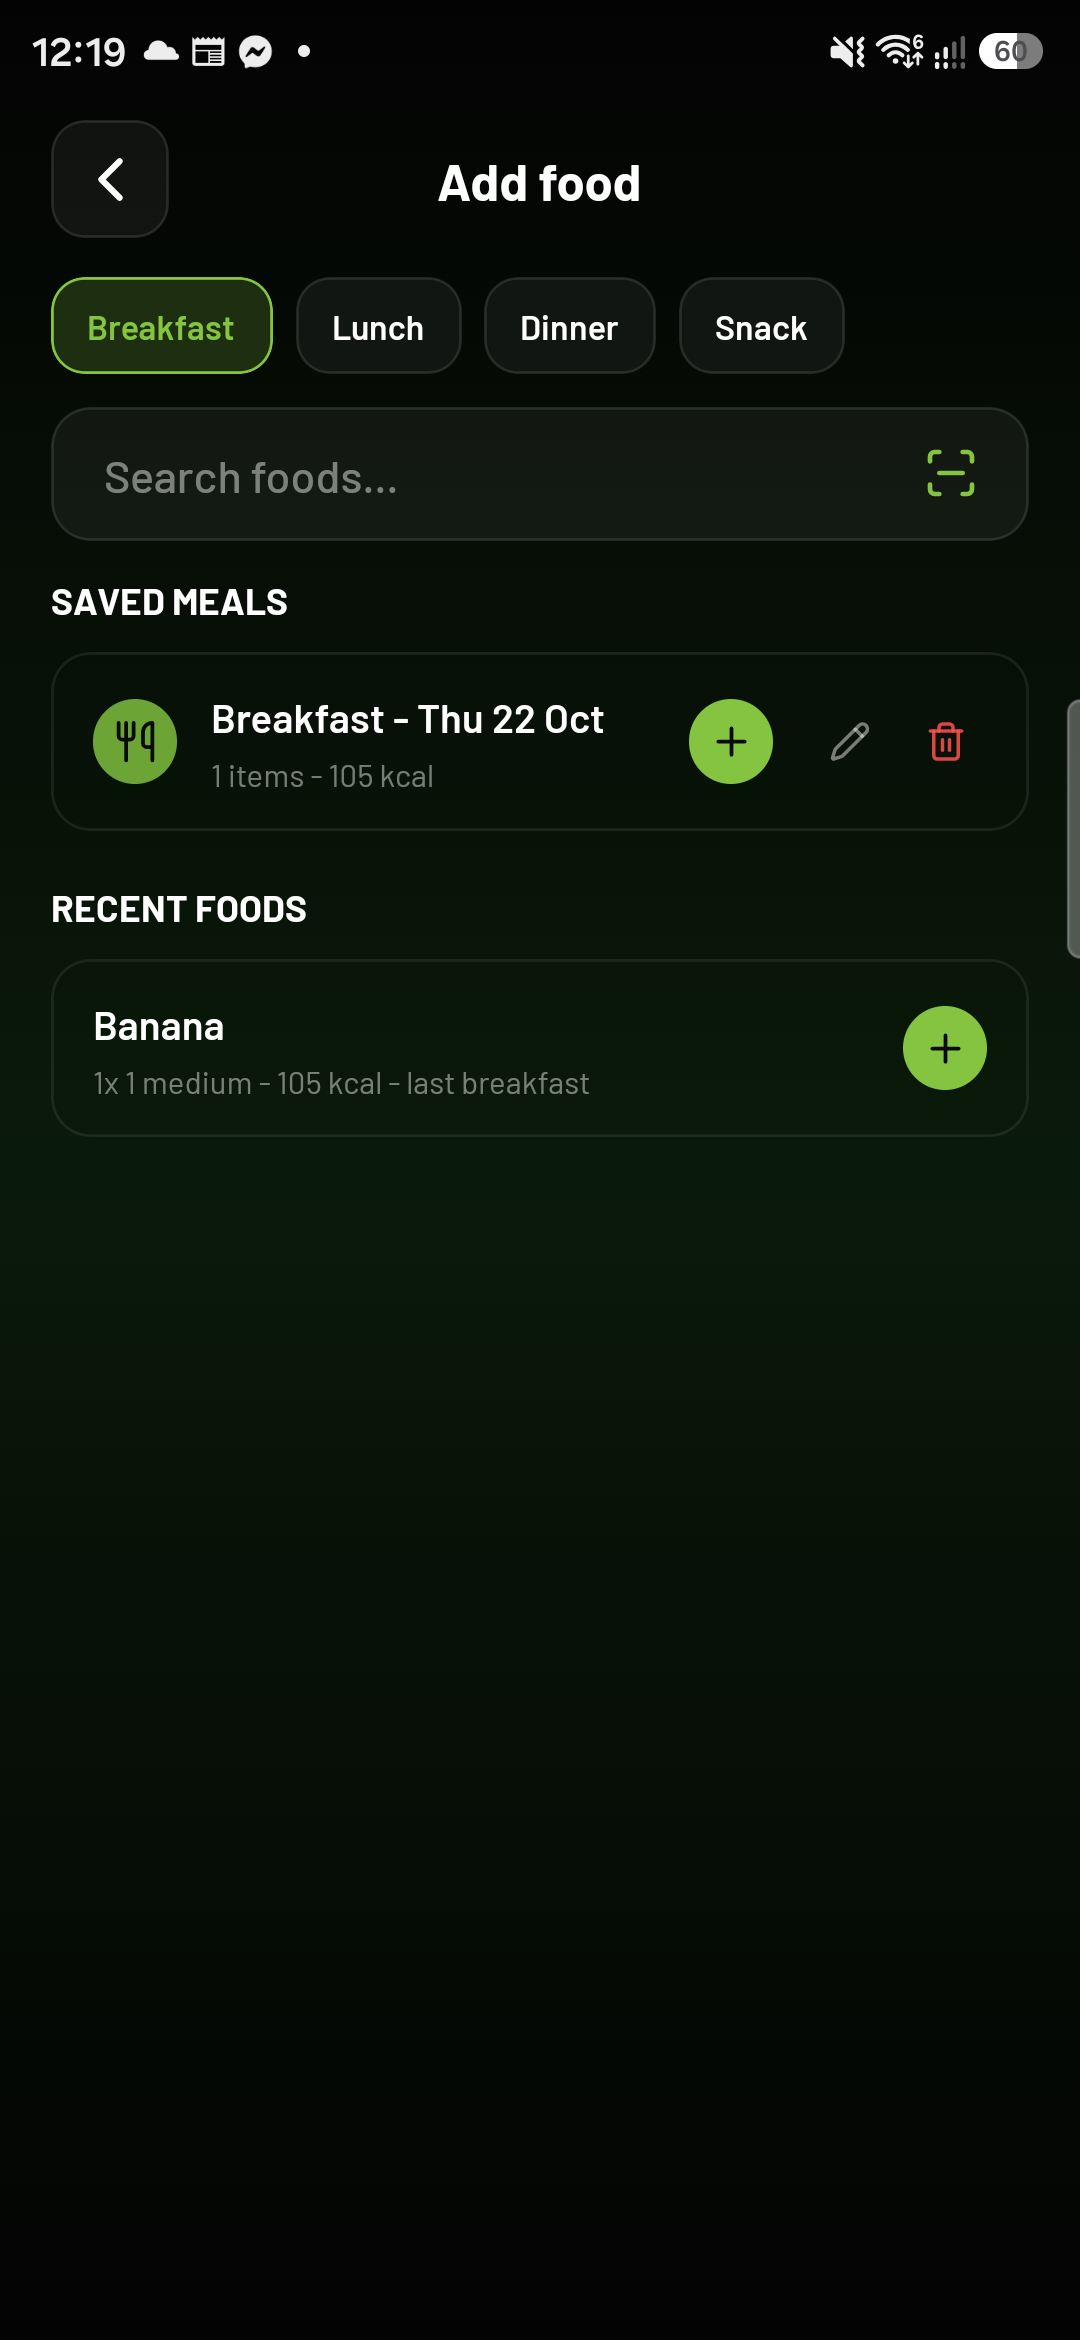
\includegraphics[width=\linewidth]{figures/screenshots/client-saved-meal.png}
\par\smallskip{\footnotesize c) Saved-meal entry\par}
\end{minipage}
\caption{Client nutrition walkthrough: goal settings, disposable food log and visible saved-meal entry.}
\label{fig:ui-nutrition-extended}
\end{figure}

\subsection{Data Interpretation and User Feedback}

A key design point in Sprint 2 is that GoFit should not only store values; it should help the user interpret them. For example, workout history becomes useful when the app can show consistency, completed sessions, training load, and trends. Body measurements become useful when the user can compare corrected values over time and understand why an AI draft may be uncertain. Nutrition entries become useful when they are reusable and connected to habits rather than isolated forms.


\subsection{Client Nutrition Preferences and Name-Based Food Filtering}

GoFit records dietary preferences, declared allergy terms and disliked foods to support food selection. The search implementation uses the recorded allergy and dislike terms as name-based exclusions; ingredient-level analysis and controlled validation would be needed to establish broader exclusion coverage.


In GoFit, the nutrition module was expanded with a robust preference architecture. The user\_profiles database table was extended with dietary\_preferences (TEXT[]), food\_allergies (TEXT[]), and food\_dislikes (TEXT[]) supported by PostgreSQL GIN indexes. During onboarding \seqsplit{(OnboardingScreenNutrition.tsx),} new users explicitly define their allergies and disliked ingredients. On the NutritionScreen, an interactive callout alerts users with incomplete dietary profiles, routing them directly to complete their configuration.


In the inspected food-search path, \texttt{AddFoodScreen} combines the saved allergy and dislike terms and passes them to \texttt{nutritionService.searchFoods}. For each non-empty term, the service adds a case-insensitive negated match against the food catalog's \texttt{name} field. This mechanism excludes names matching the supplied patterns; it does not inspect ingredient lists or establish the allergen content of a product. Ingredients absent from a product name and alternative terminology can therefore remain undetected. This search implementation alone does not establish equivalent filtering throughout recommendation workflows.

The feature is consequently described as name-based food filtering. It cannot establish that every returned item is suitable for a declared allergy. The controlled exclusion scenario remains pending in the Sprint 2 validation matrix, consistently with the limitations recorded for FR-05 in Table~\ref{tab:implementation-evidence}.


\subsection{Hydration Tracking and Multi-Period Macronutrient Analytics}

In addition to qualitative food filtering, GoFit provides comprehensive quantitative nutrition analytics. The mobile screen integrates an interactive MacroRings visualization that tracks daily calories, protein, carbohydrates, and healthy fats against personalized caloric targets. A quick-tap water intake tracker (+250ml / +500ml) encourages daily hydration. To help users focus on sustainable long-term consistency rather than single-day fluctuations, a 7-day rolling trend widget calculates average caloric intake and adherence scores across protein, water, and fiber.


The sprint therefore uses feedback patterns such as charts, summaries, empty states, warnings, and review screens. This is especially important for AI-assisted measurements. Instead of hiding uncertainty, the application should show quality issues such as poor pose, incomplete body visibility, weak segmentation, bad framing, or inconsistent scale between front and side photos.


\subsection{AI Body Measurement and Computer Vision Pipeline}

One of the most distinctive parts of GoFit is the AI-assisted body measurement feature. Its objective is to help users follow physical progress from photos, without replacing manual tape measurements and without claiming medical or tailoring-grade precision. The feature is designed as an assisted workflow: the system analyzes front and side photos, generates draft values for chest, waist, hip, and shoulder, explains capture-quality issues, then lets the user review and correct the values before saving them as progress data.


The pipeline starts on the mobile device. The user captures or selects front and side images. The application runs pose detection to locate key body landmarks, segmentation to isolate the person


silhouette when available, feature extraction to transform image geometry into measurable indicators, and a measurement estimator to produce draft values. The result is presented with confidence, warnings, and manual editing fields. This design is important because computer vision can support progress tracking, but a single two-dimensional image cannot directly recover exact body circumferences in all conditions.


\subsection{Models and Artifacts Used}

The project evolved from a keypoint-only prototype toward pose and segmentation integration. MoveNet Lightning is used through the TensorFlow Lite bridge as an initial/fallback path. MediaPipe supplies a richer landmark representation and an Android native integration; improved accuracy or speed relative to the fallback is not established by a controlled comparative benchmark.


\begingroup
\scriptsize
\setlength{\tabcolsep}{3pt}
\renewcommand{\arraystretch}{1.20}
\setlength{\LTpre}{5pt}
\setlength{\LTpost}{10pt}
\begin{longtable}{|L{2.74cm}|L{5.18cm}|L{4.18cm}|L{2.30cm}|}
\caption{AI and computer vision models used in GoFit}\label{tab:pdf-58-26} \\
\hline
\rowcolor{entetetab}
Model/artifact & Role in GoFit & Input/output & Status and reason \\ \hline
\endfirsthead
\hline
\rowcolor{entetetab}
Model/artifact & Role in GoFit & Input/output & Status and reason \\ \hline
\endhead
MoveNet Lightning (.tflite) & Initial on-device pose detection and fallback path. & Resized 192 x 192 RGB image; 17 body keypoints with confidence scores. & Implemented through \seqsplit{react-native-fast-tflite.} Useful as a lightweight baseline, but limited for body measurement because 17 keypoints do not describe torso outline or body depth. \\ \hline
MediaPipe Pose Landmarker Full (pose landmarker full.tas \_ \_ & Main candidate for richer body-pose analysis. & Image input; 33 normalized landmarks, optional world landmarks, & Implemented in the local Expo native module on Android. It improves body \\ \hline
k) &  & visibility/presence scores, pose count, and inference time. & coverage over MoveNetand supports better pose-quality checks. \\ \hline
MediaPipe Pose Landmarker Heavy & Potential higher-accuracy candidate. & Same landmark structure as the Full model, with heavier computation. & Not adopted by default. It is reserved for comparison only if Full is accurate enough and device performance remains acceptable. \\ \hline
selfie multiclass 256x256. \_ \_ tflite & Experimental segmentation research artifact. & 256 x 256 float image input; 256 x 256 x 6 class output. & Investigated but not treated as the final silhouette model because the body mask was unstable in mirror/direct capture scenarios. \\ \hline
MediaPipe Image Segmenter (selfie segmenter.tflite) \_ & Person-mask extraction for segmentation-assisted measurement. & Image input; confidence/category masks for the selected model. & Integrated in the Android native module after the earlier multiclass experiment. Comparative mask quality and effects on measurement error require controlled evaluation. \\ \hline
Statistical depth estimator & Converts extracted features into draft circumferences. & Feature vector using height, front widths, side depths, ratios, pose scores, and mask quality indicators. & Used as a pragmatic baseline. It is not a trained medical model; it produces draft progress estimates and must remain editable by the user. \\ \hline
Future regression/PCA estimator & Target research direction for stronger measurement prediction. & Labeled dataset of body features and manual/tape measurements. & Planned improvement based on statistical body-\allowbreak measurement literature. It would replace rigid formulas with learned predictors once enough validation data exists. \\ \hline
\end{longtable}
\endgroup

\subsection{Pose Detection: MoveNet and MediaPipe}

Pose detection is responsible for finding anatomical landmarks that anchor the measurement process. In the first GoFit prototype, MoveNet Lightning detects 17 keypoints such as nose, shoulders, elbows, wrists, hips, knees, and ankles. These points are enough to estimate body orientation and basic proportions, but they are not enough to measure chest, waist, and hip circumference directly. For example, a shoulder keypoint tells where the shoulder is, but it does not describe the width of the torso at chest level or the depth of the body from the side view.


The MediaPipe Pose Landmarker Full model improves this stage by producing 33 landmarks and richer metadata. The local module returns image dimensions, pose count, normalized landmarks, world landmarks when available, and inference time. The GoFit Android implementation loads the bundled \seqsplit{pose\_landmarker\_full.task} asset, decodes the image URI, applies EXIF rotation, runs MediaPipe detection, and returns a typed result to the TypeScript layer. This makes the measurement workflow more reliable because the application can inspect landmark visibility, check whether core points are present, and reject only captures that are genuinely unusable.


The project keeps MoveNet as a fallback because it is already integrated in the mobile JavaScript service and can continue to support devices or builds where the native MediaPipe module is not available. This fallback strategy reduces deployment risk while the native module reaches parity across Android and iOS.


\subsection{Segmentation and Body Mask Extraction}

Segmentation is the second computer-vision component. Its role is to separate the person from the background and provide body-outline information. This is necessary because circumference estimation cannot be based only on joint coordinates. The pose model can locate shoulder, hip, and torso reference lines; the segmentation mask can then estimate front-view widths and side-view depths around the chest, waist, and hip levels.


The project first examined \seqsplit{selfie\_multiclass\_256x256.tflite.} That model exposes a 256 x 256 x 6 output rather than a simple binary body mask, which required class selection, argmax maps, connected-component cleanup, and debugging overlays. Real tests showed that the resulting mask could be unstable, especially with mirror photos, phone occlusion, and direct capture conditions. For this reason, the report classifies it as an experimental research artifact instead of a final production model.


The later implementation uses MediaPipe Image Segmenter with \seqsplit{selfie\_segmenter.tflite} in the local native module. The Android bridge returns confidence masks, category masks, labels, quality scores, and inference timing. The TypeScript segmentation service decodes the masks, thresholds the person class, builds a cleaned binary mask, extracts sampled class grids for debugging, anchors scan lines using pose landmarks, and measures chest, waist, and hip widths/depths. This gives GoFit a more explainable measurement pipeline because each generated number can be traced back to pose landmarks, mask rows, and quality gates.


\subsection{Feature Vector and Measurement Estimation}

The measurement service builds a structured feature vector before calculating the final draft values. This is a strong architectural choice because the application does not mix raw pixels, pose confidence, segmentation quality, and final centimeter values in a single opaque formula. Instead, it records the intermediate indicators that explain why a measurement was accepted, warned, or rejected.


\begingroup
\footnotesize
\setlength{\tabcolsep}{3pt}
\renewcommand{\arraystretch}{1.20}
\setlength{\LTpre}{5pt}
\setlength{\LTpost}{10pt}
\begin{longtable}{|L{3.67cm}|L{5.29cm}|L{5.73cm}|}
\caption{Body measurement feature vector}\label{tab:pdf-61-27} \\
\hline
\rowcolor{entetetab}
Feature group & Examples & Purpose \\ \hline
\endfirsthead
\hline
\rowcolor{entetetab}
Feature group & Examples & Purpose \\ \hline
\endhead
User scale & Declared height in centimeters, person height in pixels, scale incm/px, height-span fraction. & Converts image measurements into approximate real-world dimensions and detects bad framing. \\ \hline
Pose quality & Front and side pose model source, mean landmark score, visible core keypoints, body center, top and bottom normalized positions. & Checks whether the user is visible, centered, and sufficiently detected. \\ \hline
Front geometry & Front shoulder width, hip width, estimated waist width, chest/waist/hip mask widths. & Measures visible body widths from the front photo. \\ \hline
Side geometry & Side shoulder width, side-to-front ratio, chest depth, abdomen depth, side mask depths. & Approximates body depth, which is essential for circumference estimation. \\ \hline
Segmentation quality & Raw coverage, clean coverage, body class index, mask bounds, fragmentation, class grid, person threshold. & Detects unstable masks and prevents unreliable segmentation from overriding safer estimates. \\ \hline
Estimator outputs & Draft chest, waist, hip, shoulder, depth source, confidence, failed checks, quality issues. & Produces editable progress values and explains uncertainty to the user. \\ \hline
\end{longtable}
\endgroup

The estimator combines geometric features with statistical depth assumptions. Declared height provides a scale, and front/side information contributes to draft circumference estimates. Segmentation contributes only when its quality gates accept the result; otherwise the code uses fallback assumptions. These checks are intended to reduce implausible outputs, but they do not establish numerical error bounds or prevent every incorrect estimate.


Research notes in the project also identify a stronger long-term direction: use a labeled dataset of photos and manual measurements to train regression, ridge regression, gradient-boosted trees, PCA-based, or body-shape models. Such a model would learn the relationship between extracted features and real measurements instead of relying mainly on hand-built formulas. For the PFE scope, the current implementation is correctly presented as an AI-assisted progress estimator with validation and manual correction.


The current iOS MediaPipe bridge explicitly throws not-implemented errors for pose and segmentation. The pose service selects MoveNet outside Android, but that fallback and shared TypeScript do not establish a working iOS measurement workflow or feature parity. Historical Android debug observations must therefore remain distinct from current Android inference validation, iOS support and release-build testing.

\subsection{Validation Results and Limitations}

A project troubleshooting entry dated 20 April 2026 reports Android development-client debug trials with 33 landmarks, approximate pose scores of 0.99 for a front image and 0.98 for a side image, and approximately 38/65 ms for that particular mirror-image pair. These are historical developer-recorded observations in \path{../docs/troubleshooting/BODY_MEASUREMENT_MEDIAPIPE_POSE_LANDMARKER_SPIKE.md}, not an independently reproduced October test or a population-level benchmark. Pose confidence and individual inference times do not establish circumference accuracy or end-to-end user latency.


Reliable circumference estimation remains unverified. Troubleshooting notes describe unstable masks and changing formulas, but no retained paired reference dataset establishes accuracy, repeatability or error distribution for the current version. The October QA inspected history and permission handling without completing a new front/side scan or edited-result save. User correction can improve a saved value, but it must not be counted as accuracy of the original AI estimate.


\begingroup
\footnotesize
\setlength{\tabcolsep}{3pt}
\renewcommand{\arraystretch}{1.20}
\setlength{\LTpre}{5pt}
\setlength{\LTpost}{10pt}
\begin{longtable}{|L{3.67cm}|L{5.29cm}|L{5.73cm}|}
\caption{AI measurement validation protocol}\label{tab:pdf-62-28} \\
\hline
Validation item & Expected practice & Target/interpretation \\ \hline
Reference measurements & Measure chest, waist, hip, and shoulder with a tape before comparing with the AI result. & The tape value is the reference value for validation. \\ \hline
Capture conditions & Use good lighting, full body visible, fitted clothes, front photo, side photo at approximately 90 degrees, and consistent distance. & Bad framing, loose clothing, phone occlusion, and angled mirrors must be flagged. \\ \hline
AI result & Record the draft AI value before manual correction. & Used to calculate absolute error and identify model weaknesses. \\ \hline
Manual correction & Allow the user to edit the values before saving. & Saved corrected values should match the user's real measurement. \\ \hline
Fitness-progress target & Proposed engineering acceptance targets, not measured accuracy. & Earlier illustrative errors of 8 cm for chest, 6 cm for waist/hip and 5 cm for shoulder require justification and a reference dataset before use as accepted performance criteria. \\ \hline
Confidence & Confidence must decrease when pose, segmentation, scale, or repeated-scan stability is weak. & The report should avoid claiming 100 percent confidence for unstable captures. \\ \hline
\end{longtable}
\endgroup

\begingroup
\footnotesize
\setlength{\tabcolsep}{3pt}
\renewcommand{\arraystretch}{1.20}
\setlength{\LTpre}{5pt}
\setlength{\LTpost}{10pt}
\begin{longtable}{|L{3.67cm}|L{5.29cm}|L{5.73cm}|}
\caption{AI implementation status}\label{tab:pdf-63-29} \\
\hline
\rowcolor{entetetab}
Component & Current status & Remaining work \\ \hline
\endfirsthead
\hline
\rowcolor{entetetab}
Component & Current status & Remaining work \\ \hline
\endhead
MoveNet pose fallback & Implemented in TypeScript service through \seqsplit{react-native-fast-tflite} and bundled model asset. & Keep as fallback and compare against MediaPipe outputs. \\ \hline
MediaPipe pose Android module & Implemented with bundled pose landmarker full.task, EXIF \_ \_ rotation handling, 33 landmarks, world landmarks, pose count, and inference time. & Complete parity and production testing across iOS and Android release builds. \\ \hline
MediaPipe image segmentation & Implemented in native module with selfie segmenter.tflite, \_ confidence/category masks, labels, and quality scores. & Improve segmentation quality gates and verify on more body types, clothes, lighting, and camera setups. \\ \hline
Feature vector & Implemented with pose, scale, geometry, segmentation, confidence, and debug fields. & Export validation datasets and compare AI estimates with tape measurements. \\ \hline
Estimator & Statistical baseline and segmentation-gated depth source available. & Train or calibrate a stronger model once enough labeled examples exist. \\ \hline
User workflow & Draft measurement, quality warnings, and manual review approach defined. & Finalize UX copy, screenshots, and submission-ready validation evidence. \\ \hline
\end{longtable}
\endgroup

In conclusion, the AI module is a meaningful technical contribution because it combines on-device inference, native module integration, pose landmarks, segmentation masks, typed feature vectors, statistical estimation, and validation methodology. At the same time, the report must be transparent: GoFit uses AI to assist progress tracking, not to replace professional body measurement.


Figure~\ref{fig:ui-measurement-boundary} presents cropped measurement guidance and the observed camera-denial response. It supplies no fresh inference, review/save or numerical-accuracy result. A successful measurement draft and an independent accuracy comparison remain missing evidence.

\begin{figure}[H]
\centering
\begin{minipage}[t]{.42\linewidth}
\centering
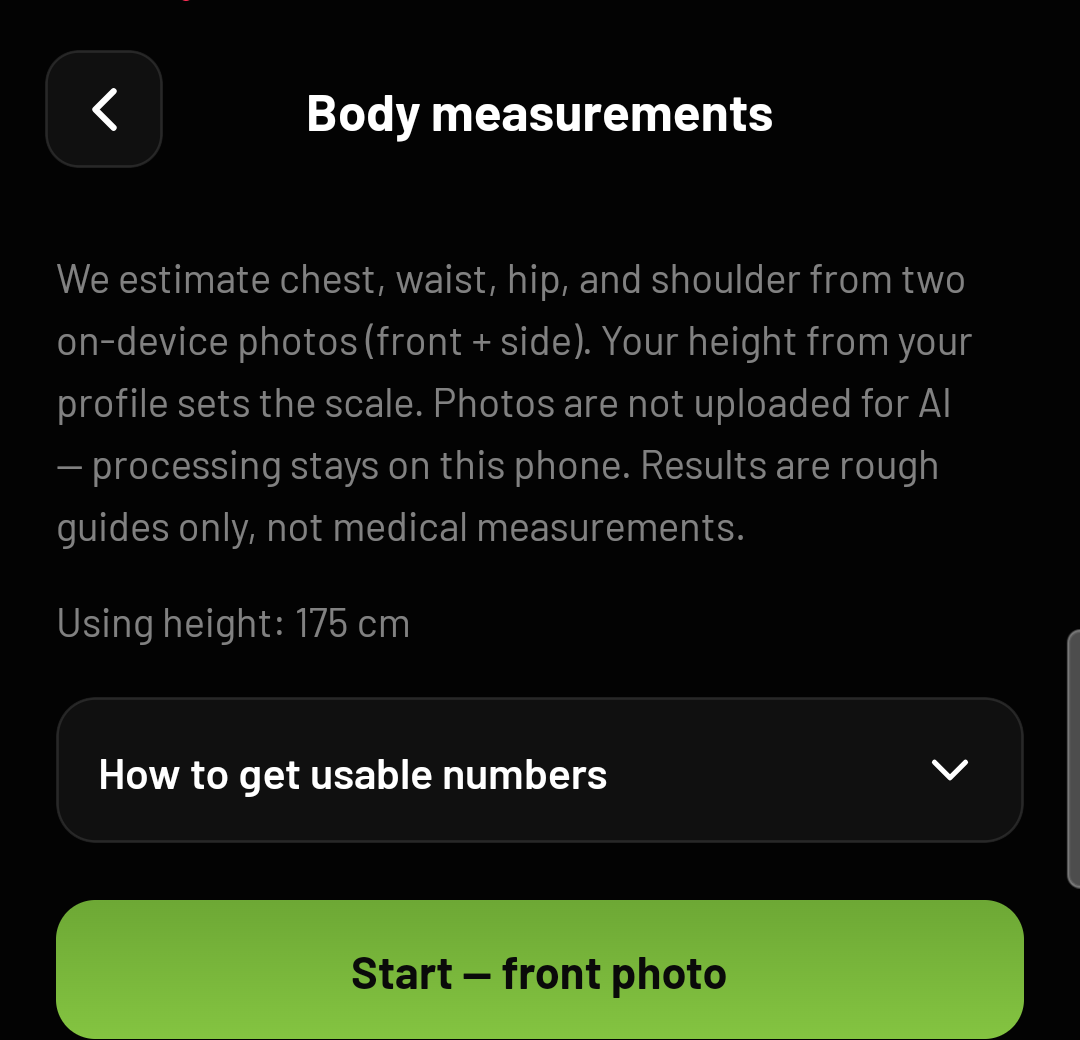
\includegraphics[width=\linewidth,height=8.5cm,keepaspectratio]{figures/screenshots/measurement-guidance-excerpt.png}
\par\smallskip{\footnotesize a) Capture guidance excerpt\par}
\end{minipage}
\hspace{0.025\linewidth}
\begin{minipage}[t]{.42\linewidth}
\centering
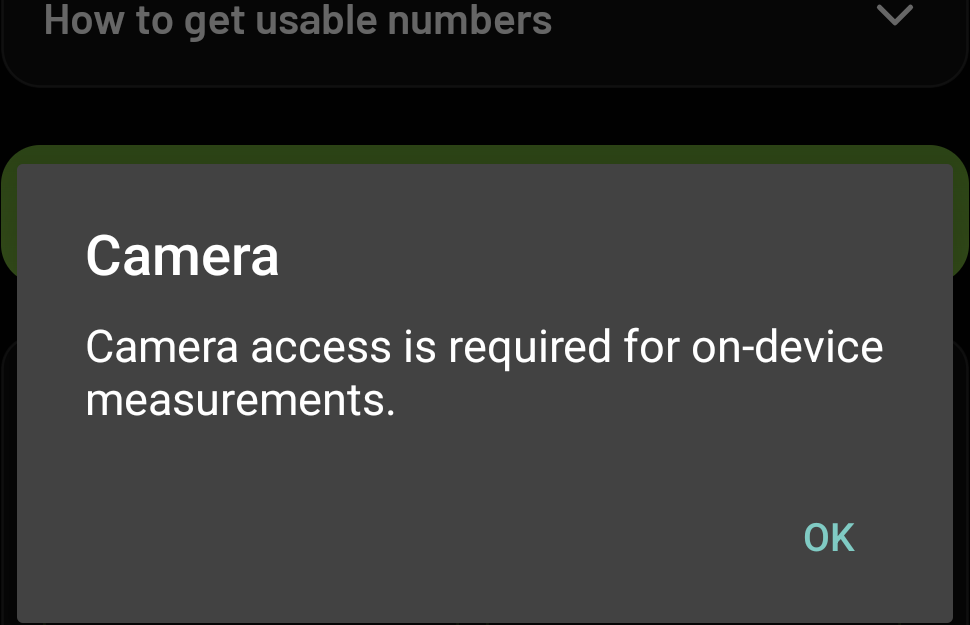
\includegraphics[width=\linewidth,height=8.5cm,keepaspectratio]{figures/screenshots/measurement-permission-result.png}
\par\smallskip{\footnotesize b) Permission-denial message\par}
\end{minipage}
\caption{Interface excerpts: measurement guidance and handled camera denial; no successful scan is claimed.}
\label{fig:ui-measurement-boundary}
\end{figure}

\section{Tests}

This matrix reconciles the original test identifiers with the retained 22--24 October evidence; it is not a recovered sprint-period execution log. Expected outcomes remain test criteria. Partial denotes narrower observations, Pending denotes an unverified full scenario, and Scoped pass applies only to the named sandbox case. M references identify Table~\ref{tab:implementation-evidence} and its detailed index; C, A, P and S identify the evidence package in Section~\ref{sec:qa-evidence}. No missing attachment is replaced by an assumed success.


\begingroup
\scriptsize
\setlength{\tabcolsep}{2pt}
\renewcommand{\arraystretch}{1.20}
\setlength{\LTpre}{5pt}
\setlength{\LTpost}{10pt}
\begin{longtable}{|L{1.20cm}|L{1.50cm}|L{1.60cm}|L{1.60cm}|L{1.80cm}|L{1.80cm}|L{1.65cm}|L{1.35cm}|L{2.00cm}|}
\caption{Sprint validation matrix}\label{tab:pdf-64-30} \\
\hline
\rowcolor{entetetab}
Test ID & Feature & Scenario & Preconditions & Steps & Expected & Actual & Status & Evidence \\ \hline
\endfirsthead
\hline
\rowcolor{entetetab}
Test ID & Feature & Scenario & Preconditions & Steps & Expected & Actual & Status & Evidence \\ \hline
\endhead
S2-T01 & Catalog & Search and equipment filters & Populated catalog & Search; select filters & Matching exercises & Browsing passed; filters partial & Partial & M03; C LIBRARY-01--02, EXERCISE-01--04 \\ \hline
S2-T02 & Progress & Charts and aggregates & Saved session history & Open charts; compare totals & Metrics match source records & Controls viewed; arithmetic incomplete & Partial & M07; C PROGRESS-01--03 \\ \hline
S2-T03 & Measurements & Fresh capture, review and save & Camera; height; reference values & Capture pair; edit; save & Reviewed draft persisted & Fresh workflow not retained & Pending & M08; final QA-04; debug notes are narrower \\ \hline
S2-T04 & Exclusions & Name exclusion search & Controlled preference fixture & Search known included\slash{}excluded names & Expected name matches omitted & Controlled fixture not run & Pending & M09; no allergen-safety result \\ \hline
S2-T05 & Barcode & Lookup and meal logging & Camera; known product & Scan; resolve; log serving & Product and meal persisted & Permission denial only observed & Pending & M09; C NUTRITION-07; positive lookup unverified \\ \hline
S2-T06 & AI workout & Generate, review and save & Reachable recommendation entry & Request; inspect; accept; reopen & Valid saved recommendation & Entry blocked on tested account & Pending & M19; C AI-01--03; final QA-05 \\ \hline
\end{longtable}
\endgroup

\section{Progress Tracking and Evidence Limits}

The retained backlog provides planned tasks and estimates, but no dated series of remaining work, scope changes or accepted completions is available for this report scope group. A burn-down chart and measured velocity cannot be reconstructed from the current source tree or later QA outcomes. No chart is therefore presented as evidence of sprint performance. The validation matrix reports the narrower implementation and execution evidence instead.


\phantomsection
\section*{Conclusion}

This chapter connected the workout foundation to progress records, nutrition data and assisted measurement drafts. The cumulative model retains the earlier workout concepts, while the measurement and nutrition sequences distinguish local processing, review and persistence. Display and permission observations remain narrower than fresh inference, numerical accuracy, positive barcode resolution or generated-workout validation. The next chapter examines coaching and administration without treating these pending checks as completed prerequisites.


\chapter{Sprint 3}


\phantomsection
\section*{Introduction}
\addcontentsline{toc}{section}{Introduction}

The Sprint 3 scope concerns marketplace discovery, coach-client follow-up, purchases and appointments, communication components, coach-facing AI briefings and web administration. It separates these implementation paths from retained sandbox payment evidence and the outstanding booking, media, automation and administrative checks.


This chapter examines the scope designated Sprint 3 through planned tasks, cumulative domain views, selected use cases and interaction sequences, implementation descriptions and reconciled validation criteria. The models project the inspected implementation, while the retained October observations are later evidence. The closing management subsection states the limits of available progress-tracking data.


\section{Needs Assessment}

The sprint needs were selected from the prioritized product backlog according to dependency order, business value, and architectural feasibility. The following table provides a comprehensive decomposition of each user story into technical modeling, implementation, and testing subtasks.


The Sprint 3 objective is to connect client, coach and administrator activities through shared records and controlled service boundaries. Its backlog remains a statement of planned work; the dated payment follow-up and scoped QA results are assessed separately.


\subsection{Sprint Backlog}

\begingroup
\scriptsize
\setlength{\tabcolsep}{3pt}
\renewcommand{\arraystretch}{1.20}
\setlength{\LTpre}{5pt}
\setlength{\LTpost}{10pt}
\begin{longtable}{|L{1.20cm}|L{2.00cm}|L{5.40cm}|L{1.80cm}|L{4.00cm}|}
\caption{Sprint 3 backlog decomposition}\label{tab:pdf-66-31} \\
\hline
\rowcolor{entetetab}
ID US & As & User Story & Id task & Task \\ \hline
\endfirsthead
\hline
\rowcolor{entetetab}
ID US & As & User Story & Id task & Task \\ \hline
\endhead
US-5.1 & Client & Search accredited coaches, purchase session packs via Stripe, and book 1-on-1 coaching consultations & T5.1.1 & Model CoachProfile, SessionPack, PurchasedPack, and Booking entities with Stripe checkout schema. \\ \hline
US-5.1 & Client & Search accredited coaches, purchase session packs via Stripe, and book 1-on-1 coaching consultations & T5.1.2 & Implement CoachMarketplaceSc reen, CoachProfileScreen, Stripe PaymentSheet integration, and BookingCalendarScr een. \\ \hline
US-5.1 & Client & Search accredited coaches, purchase session packs via Stripe, and book 1-on-1 coaching consultations & T5.1.3 & Test Stripe payment intent creation, webhook idempotent fulfillment, and slot collision prevention. \\ \hline
US-5.2 & Coach & Dedicated mobile workspace to manage client rosters, assign tailoredworkout/meal plans, and review check-ins & T5.2.1 & Design ClientCoachAssignm ent, CheckInSubmission,and CoachNote database tables with RLS policies. \\ \hline
US-5.2 & Coach & Dedicated mobile workspace to manage client rosters, assign tailoredworkout/meal plans, and review check-ins & T5.2.2 & Implement CoachDashboardScr een, ClientListScreen, ClientDetailScreen,and PlanAssignmentScre en. \\ \hline
US-5.2 & Coach & Dedicated mobile workspace to manage client rosters, assign tailoredworkout/meal plans, and review check-ins & T5.2.3 & Verify coach-client data isolation, check-in photo review, and coach notes persistence. \\ \hline
US-5.3 & Coach/Client & Real-time encrypted messaging and low-latency 1-on-1 video consultations with AI session summaries & T5.3.1 & Model Conversation, Message, and VideoSession schema integrated with LiveKit SFU and Edge Function ai-session-notes. \\ \hline
US-5.3 & Coach/Client & Real-time encrypted messaging and low-latency 1-on-1 video consultations with AI session summaries & T5.3.2 & Implement RealtimeChatScreen (Supabase channels), LiveKitVideoScreen,and post-session AI summary card. \\ \hline
US-5.3 & Coach/Client & Real-time encrypted messaging and low-latency 1-on-1 video consultations with AI session summaries & T5.3.3 & Test WebSocket real-time delivery, LiveKit WebRTCaudio/video token generation, and Groq AI session synthesis. \\ \hline
US-5.4 & Admin & Web administration dashboard to audit coaches, manage exercise taxonomies, inspect transactions, and monitor platform BI & T5.4.1 & Design Next.js App Router architecture with Supabase service-role client and audit logs table. \_ \\ \hline
US-5.4 & Admin & Web administration dashboard to audit coaches, manage exercise taxonomies, inspect transactions, and monitor platform BI & T5.4.2 & Implement Admin Dashboard, Coach Accreditation Review (CV/certificate preview), Exercise CRUD, and Transaction Ledger. \\ \hline
US-5.4 & Admin & Web administration dashboard to audit coaches, manage exercise taxonomies, inspect transactions, and monitor platform BI & T5.4.3 & Validate Next.js middleware RBAC protection, coach document signed URLs, and system metric aggregation queries. \\ \hline
\end{longtable}
\endgroup

The original task wording remains a target, not a completion claim. US-5.1 maps to offers, purchases and bookings; the updated sequences below describe the October EUR follow-up rather than proving those corrections existed during the internship. US-5.2 maps to programs, schedules, responses and private notes; no separate ClientCoachAssignment entity is needed by this selected model, and a populated photo-review workflow remains unverified. US-5.3 maps to Conversation, Message and AISessionNote; briefing generation is distinct from post-consultation synthesis. US-5.4 maps to profile-based administrator authorization and selected audit records. The presence of those records does not imply that coach approval emits an audit or notification event. See Table~\ref{tab:sprint-traceability}.

\subsection{Sprint Class Diagram}

The Sprint 3 backlog states development and verification targets, not completed results. The current payment implementation does not supply the webhook fulfilment targeted by T5.1.3. US-5.3's post-session summaries and proposed VideoSession schema differ from the implemented coach-facing briefing and runtime video-token path; the model below reflects the inspected records. Its use of encrypted messaging remains a security requirement whose scope requires separate verification. Likewise, T5.4.3's signed-document test is a target: the inspected coach-review page opens existing document URLs. No independent professional accreditation, measured video latency, or successful execution of these tests is established by the backlog.

The Sprint 3 cumulative domain model retains the workout foundation in Figure~\ref{fig:class_sprint2_foundation} and the profile, progress, and nutrition extensions in Figure~\ref{fig:class_sprint2}. Four complementary views add the coaching and administrative concepts, reusing the same account, coach, and booking identities. Figure~\ref{fig:class_sprint3} presents the marketplace: CoachProfile belongs to an authentication account, while certifications, availability, and session packs are separate records. PurchasedPack represents a client's purchase of an offer; Booking records a scheduled session and may optionally reference that purchase. Figure~\ref{fig:class_sprint3_communication} separates conversations and messages from manual client notes and AI briefings. Figure~\ref{fig:class_sprint3_followup} represents programs, check-in schedules, and responses. Figure~\ref{fig:class_sprint3_finance} presents wallet transactions and administrative audit records. These views extend rather than replace the earlier domain model; selected attributes are shown to preserve readability.

Programs may be templates without an assigned client. Check-in responses identify a coach and client but do not require a foreign key to a schedule, and AI briefings are not necessarily linked to a booking or a recorded consultation. Video-room identity is optional booking data, while access tokens are generated at runtime. Administrator authorization uses the existing profile's is\_admin field; it does not introduce a separate AdminUser entity. Audit records describe supported logged actions, without implying that every administrative operation produces an entry. Likewise, the domain model does not establish payment settlement, end-to-end message encryption, or successful video-call validation.


\begin{figure}[H]
\centering
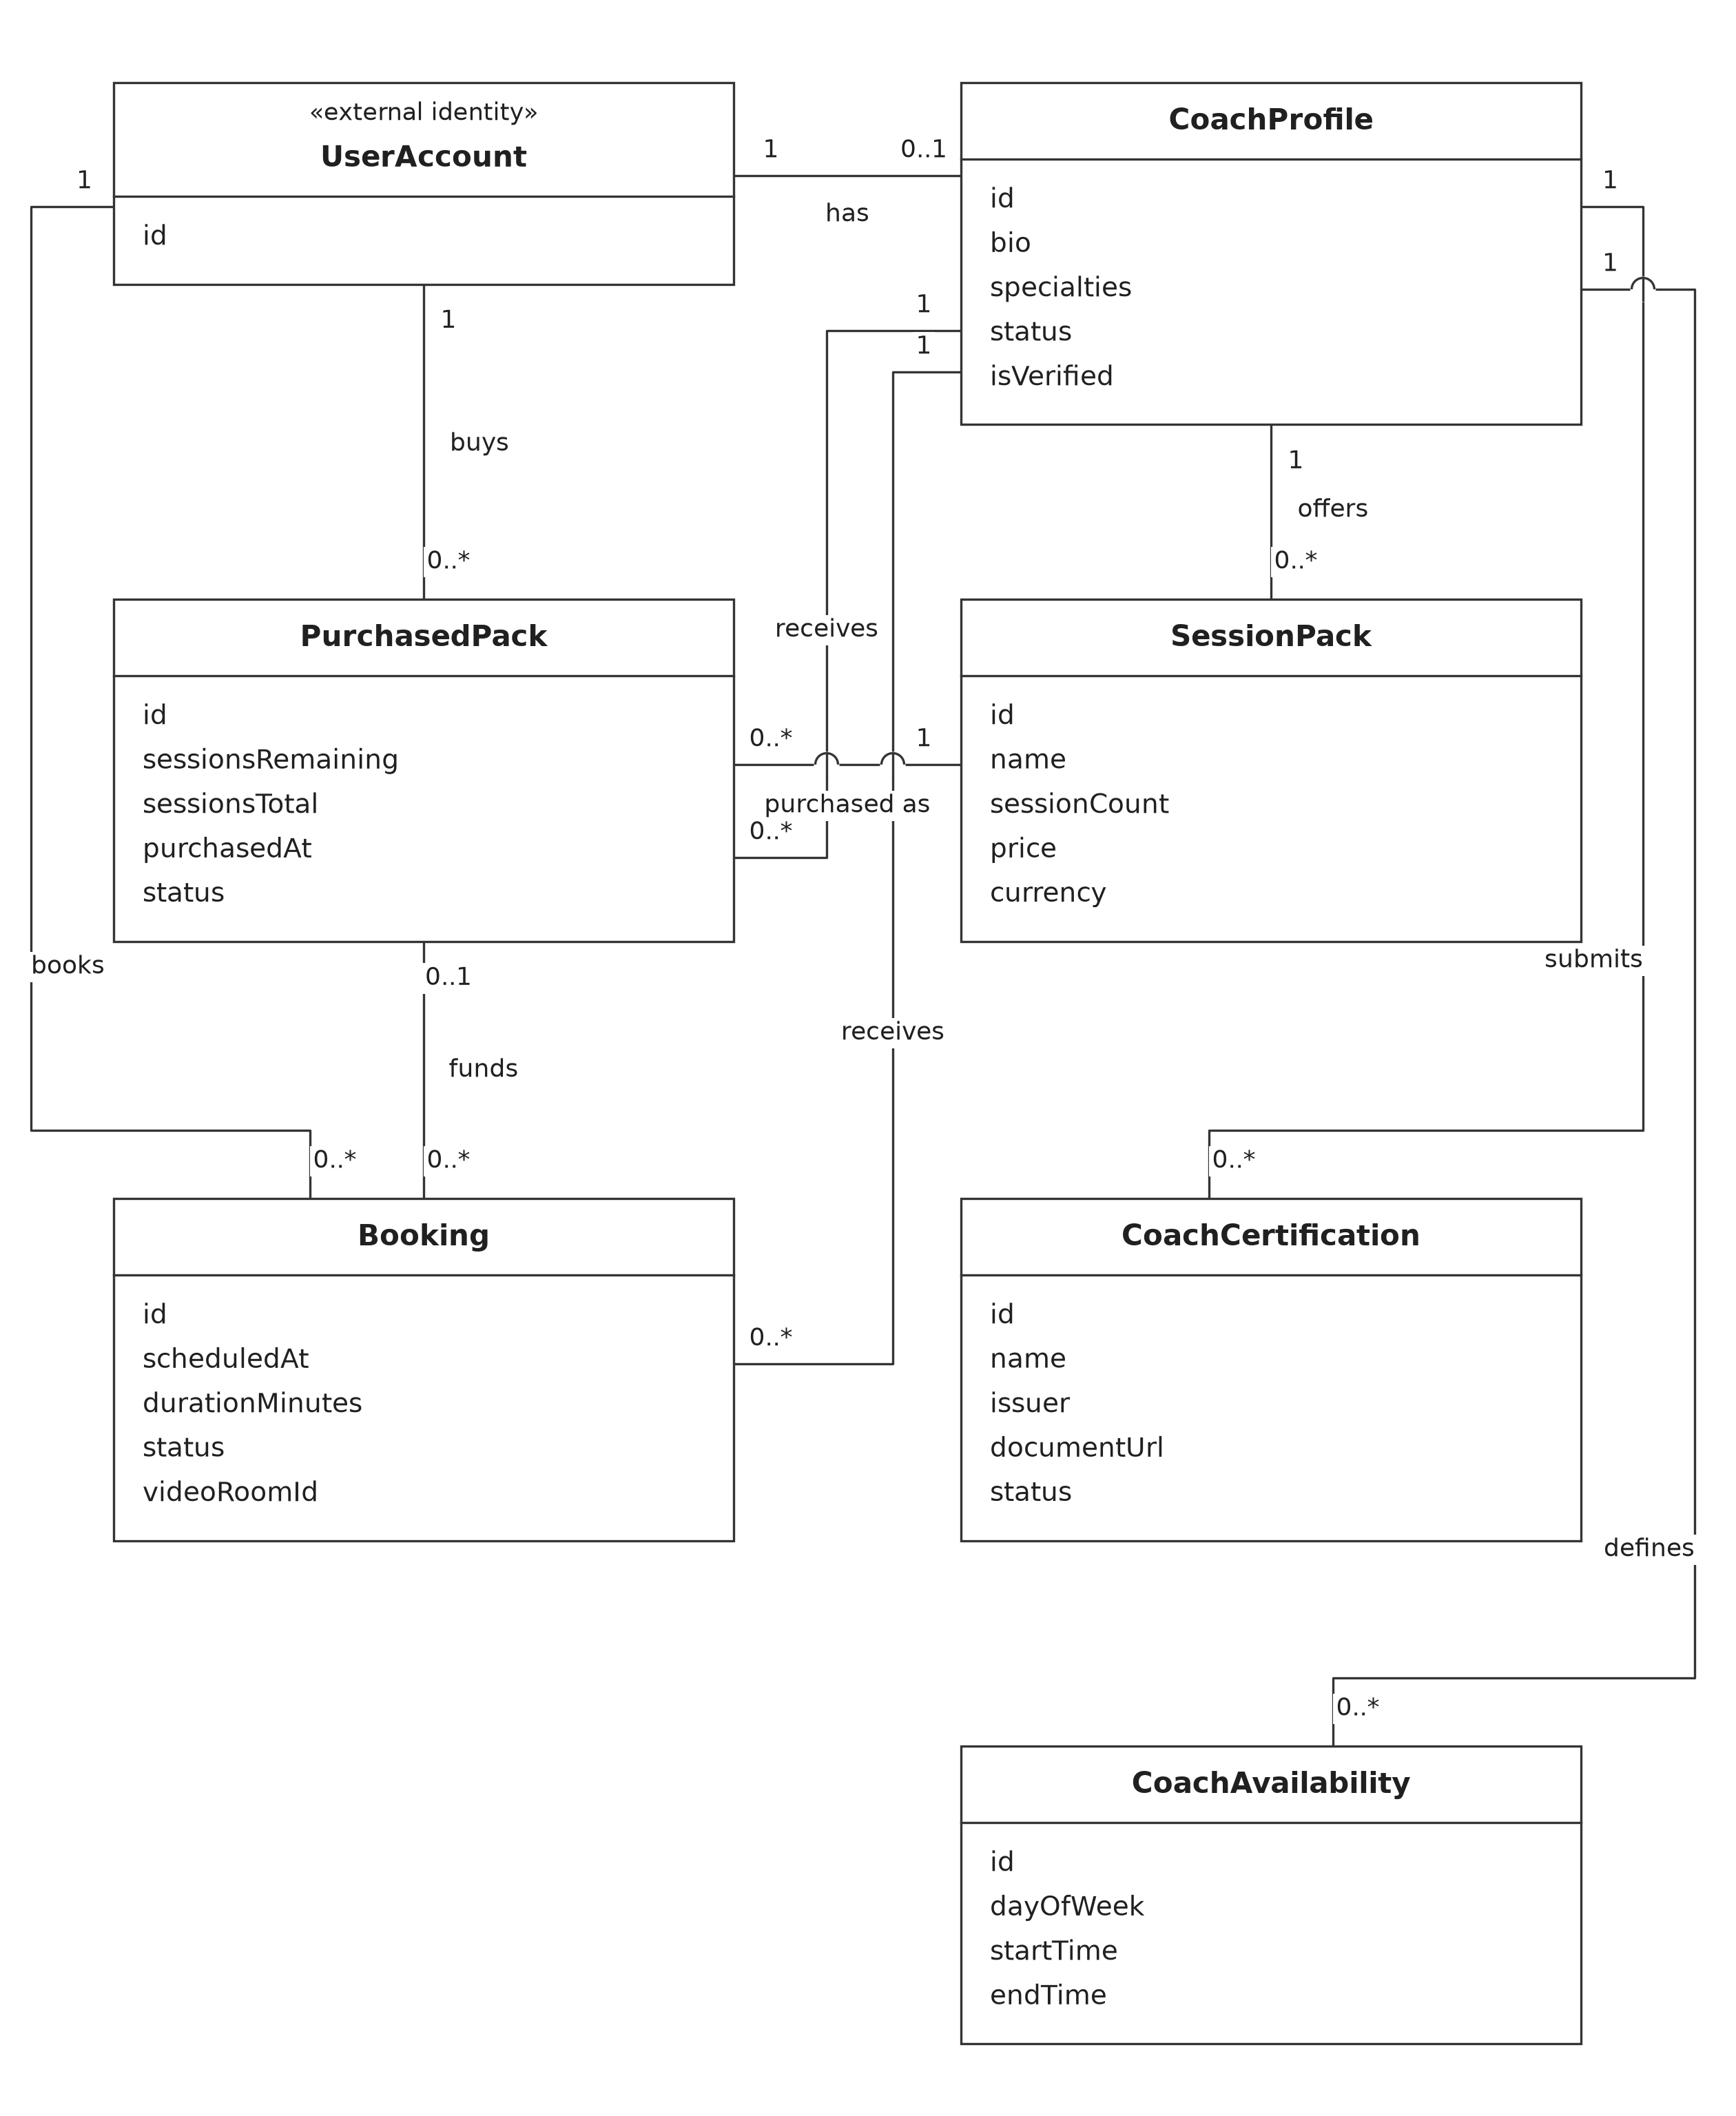
\includegraphics[width=0.95\linewidth]{figures/class_diagram_sprint3.png}
\caption{Sprint 3 cumulative domain model: marketplace and bookings}
\label{fig:class_sprint3}
\end{figure}

\begin{figure}[H]
\centering
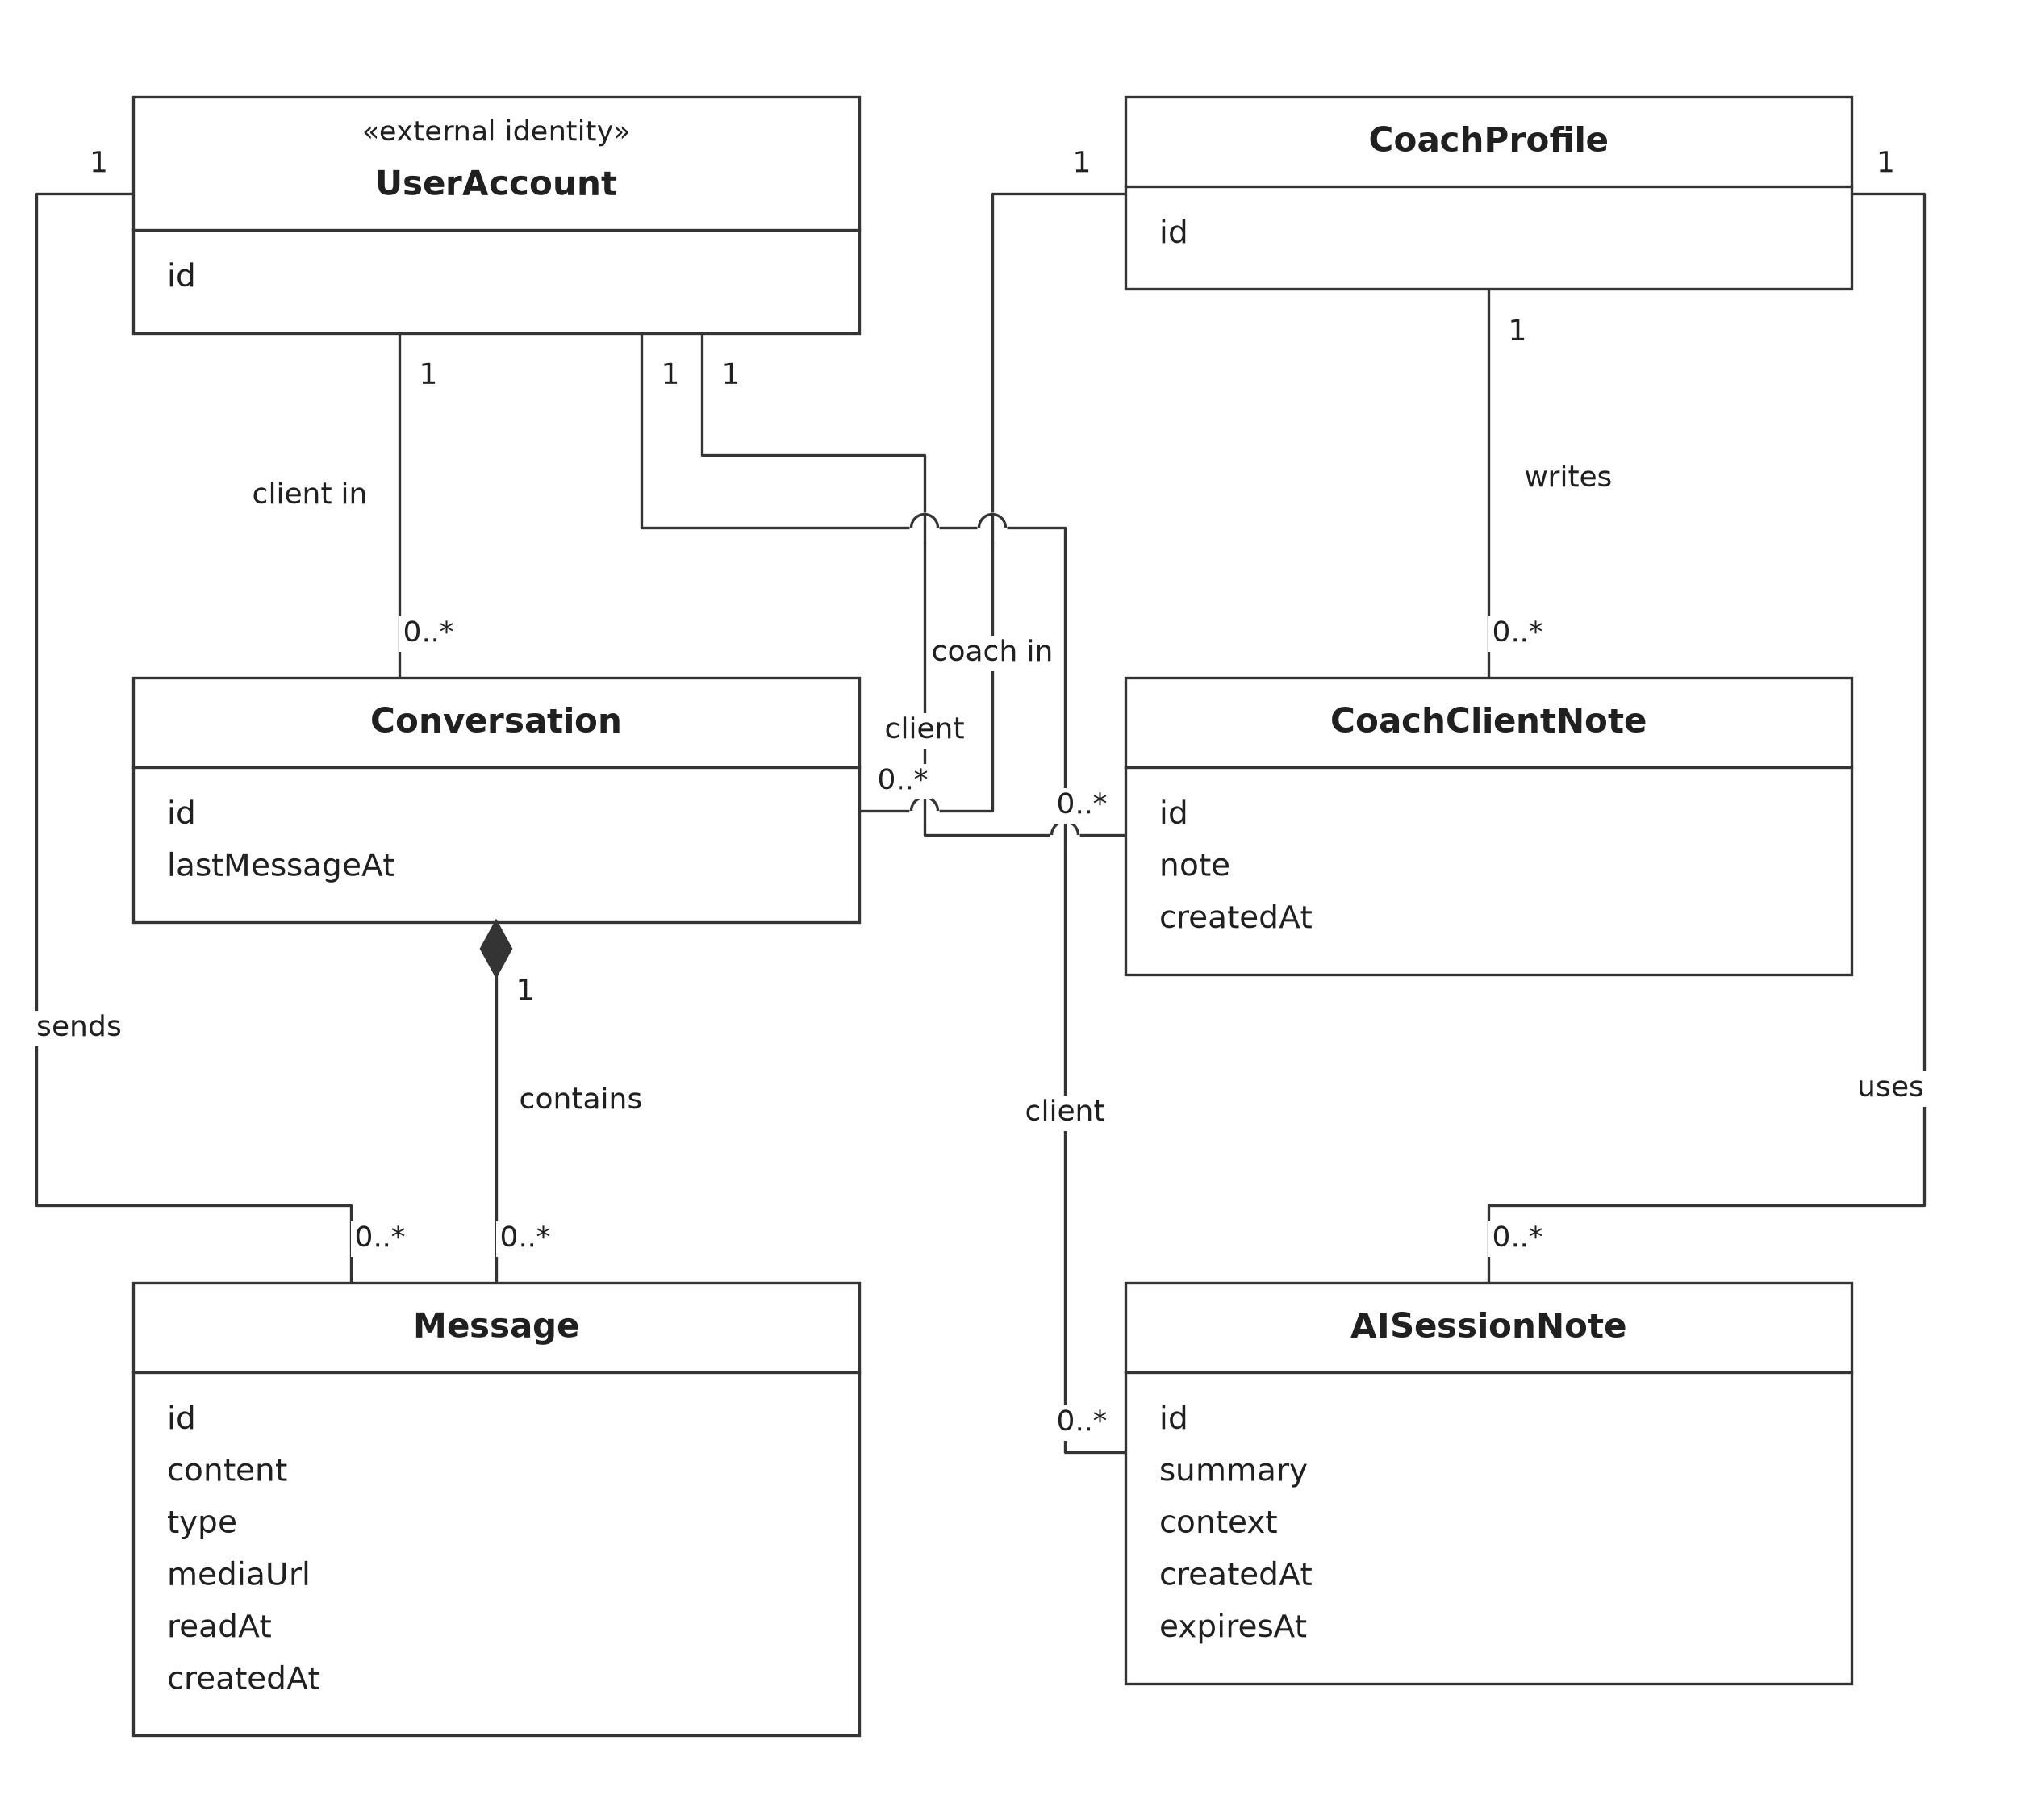
\includegraphics[width=0.95\linewidth]{figures/class_diagram_sprint3_communication.png}
\caption{Sprint 3 cumulative domain model: communication and notes}
\label{fig:class_sprint3_communication}
\end{figure}

\begin{figure}[H]
\centering
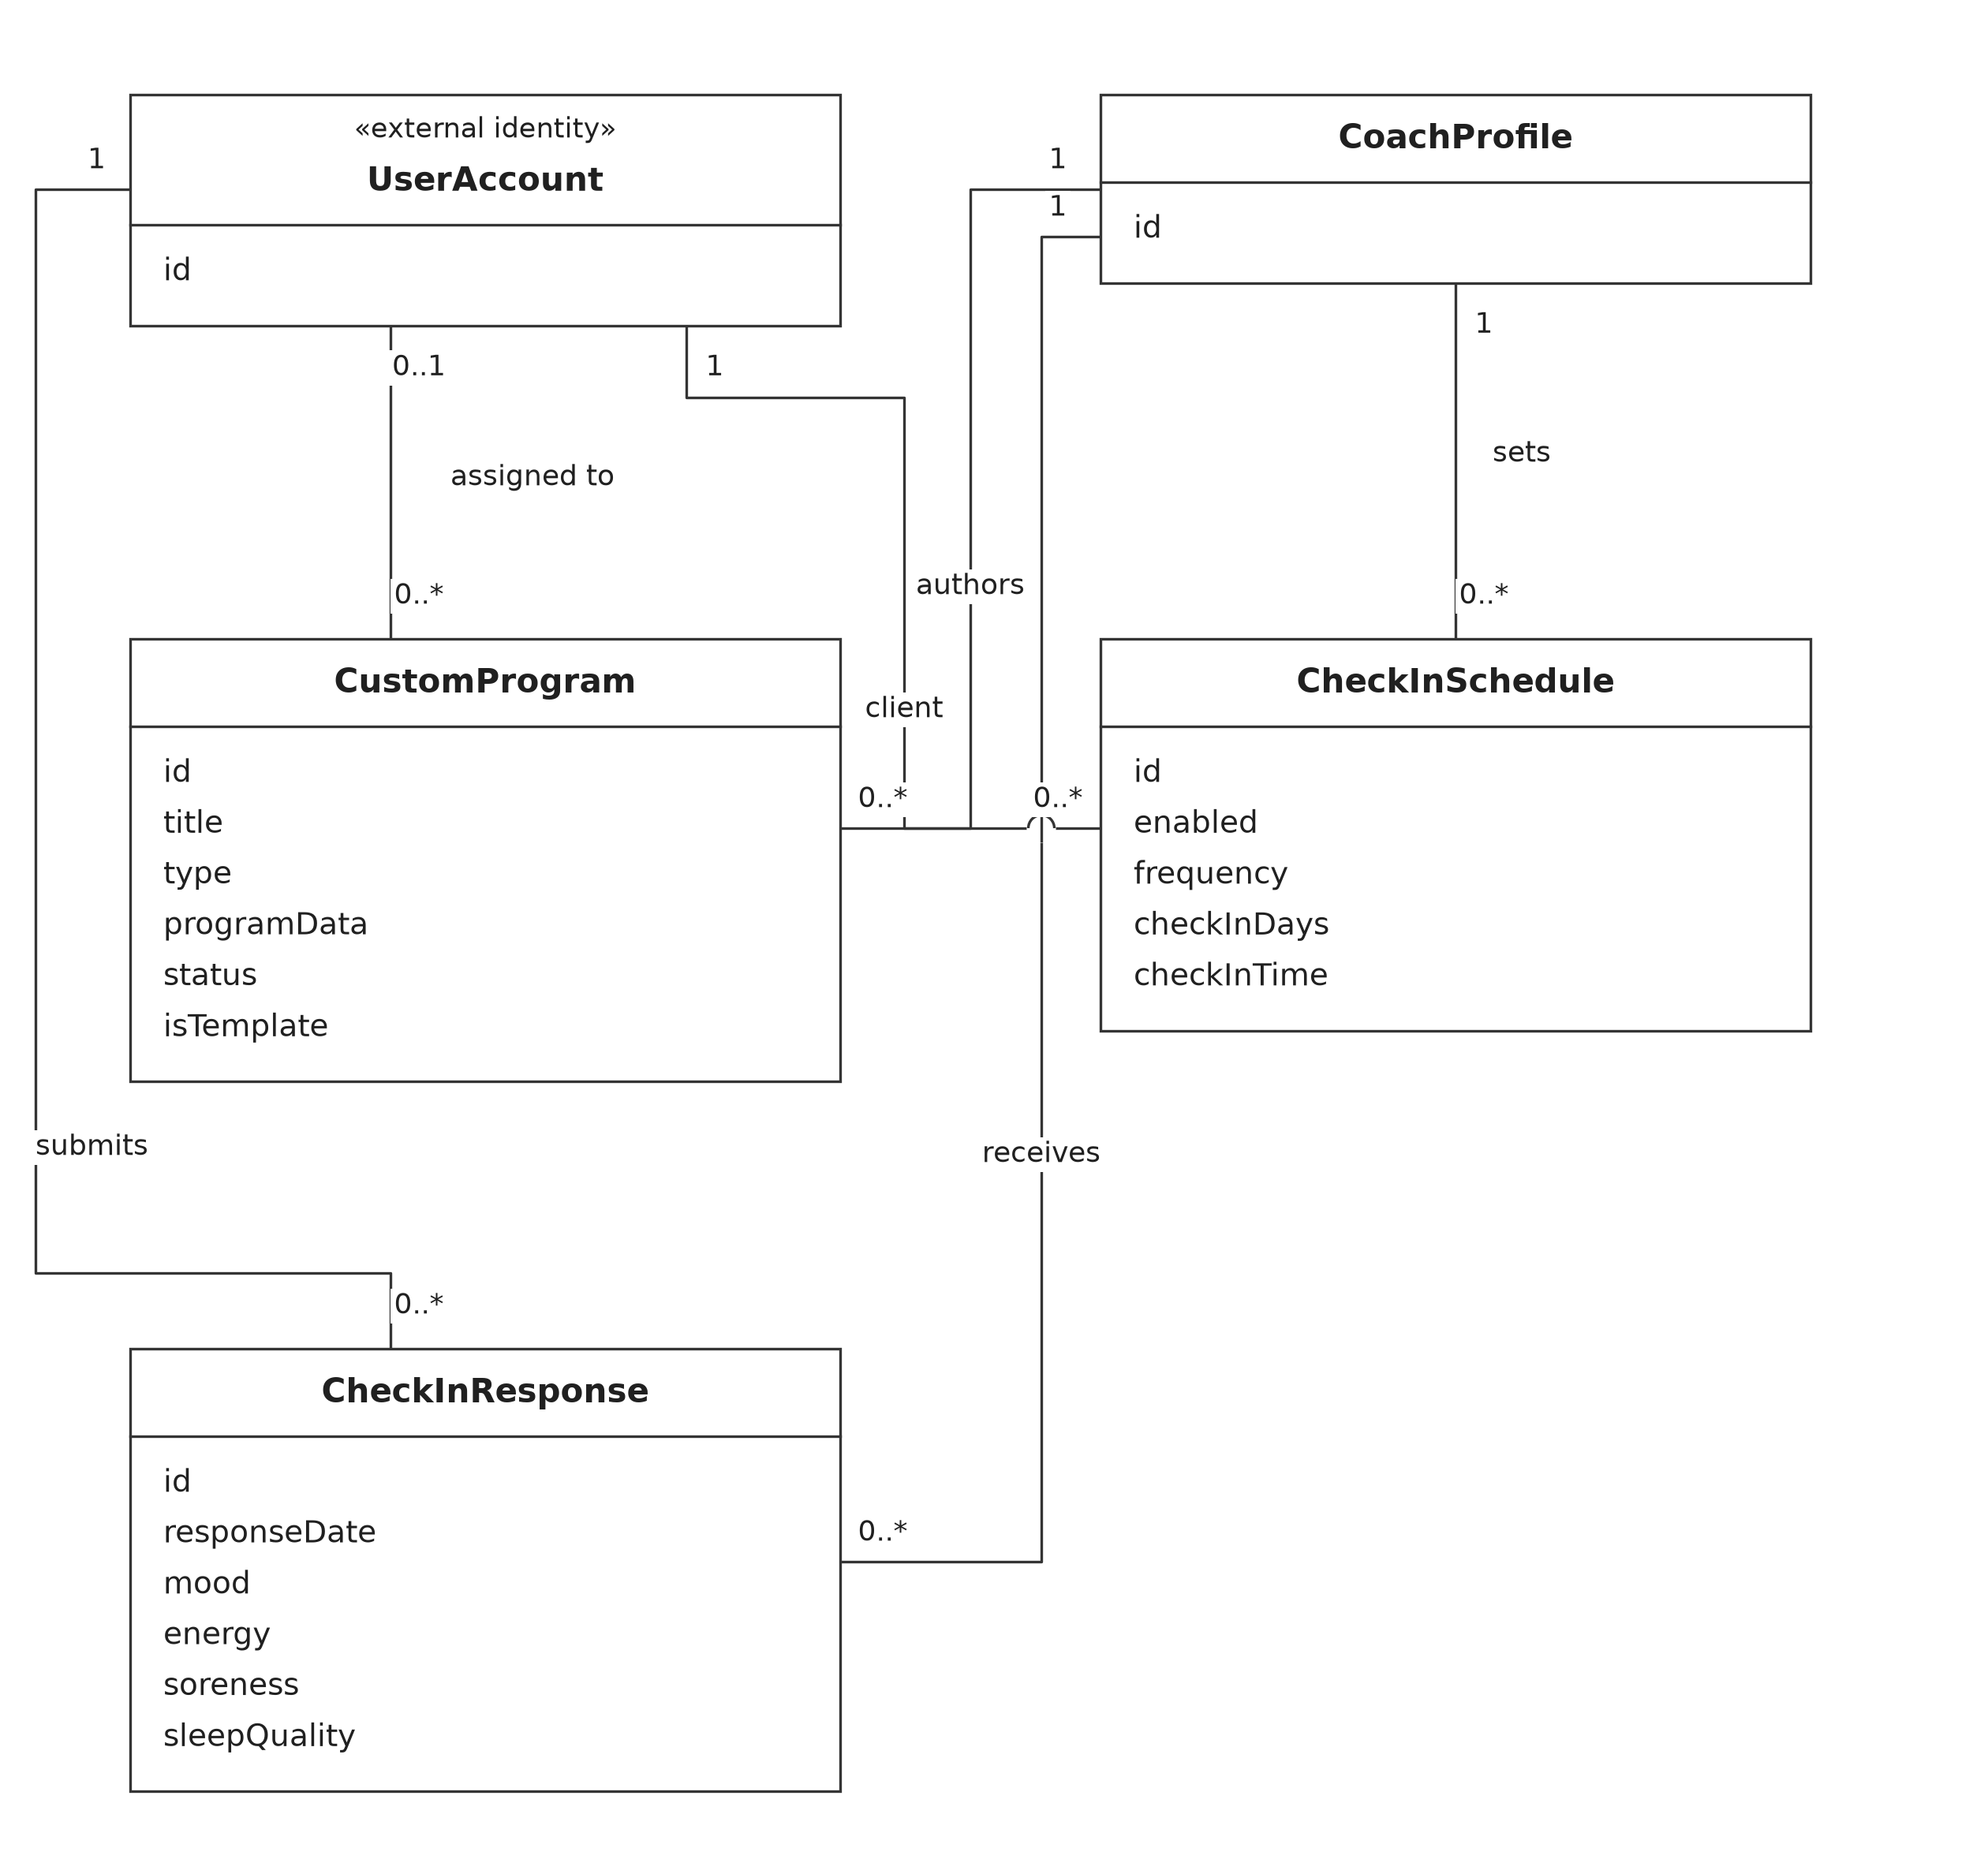
\includegraphics[width=0.95\linewidth]{figures/class_diagram_sprint3_followup.png}
\caption{Sprint 3 cumulative domain model: programs and check-ins}
\label{fig:class_sprint3_followup}
\end{figure}

\begin{figure}[H]
\centering
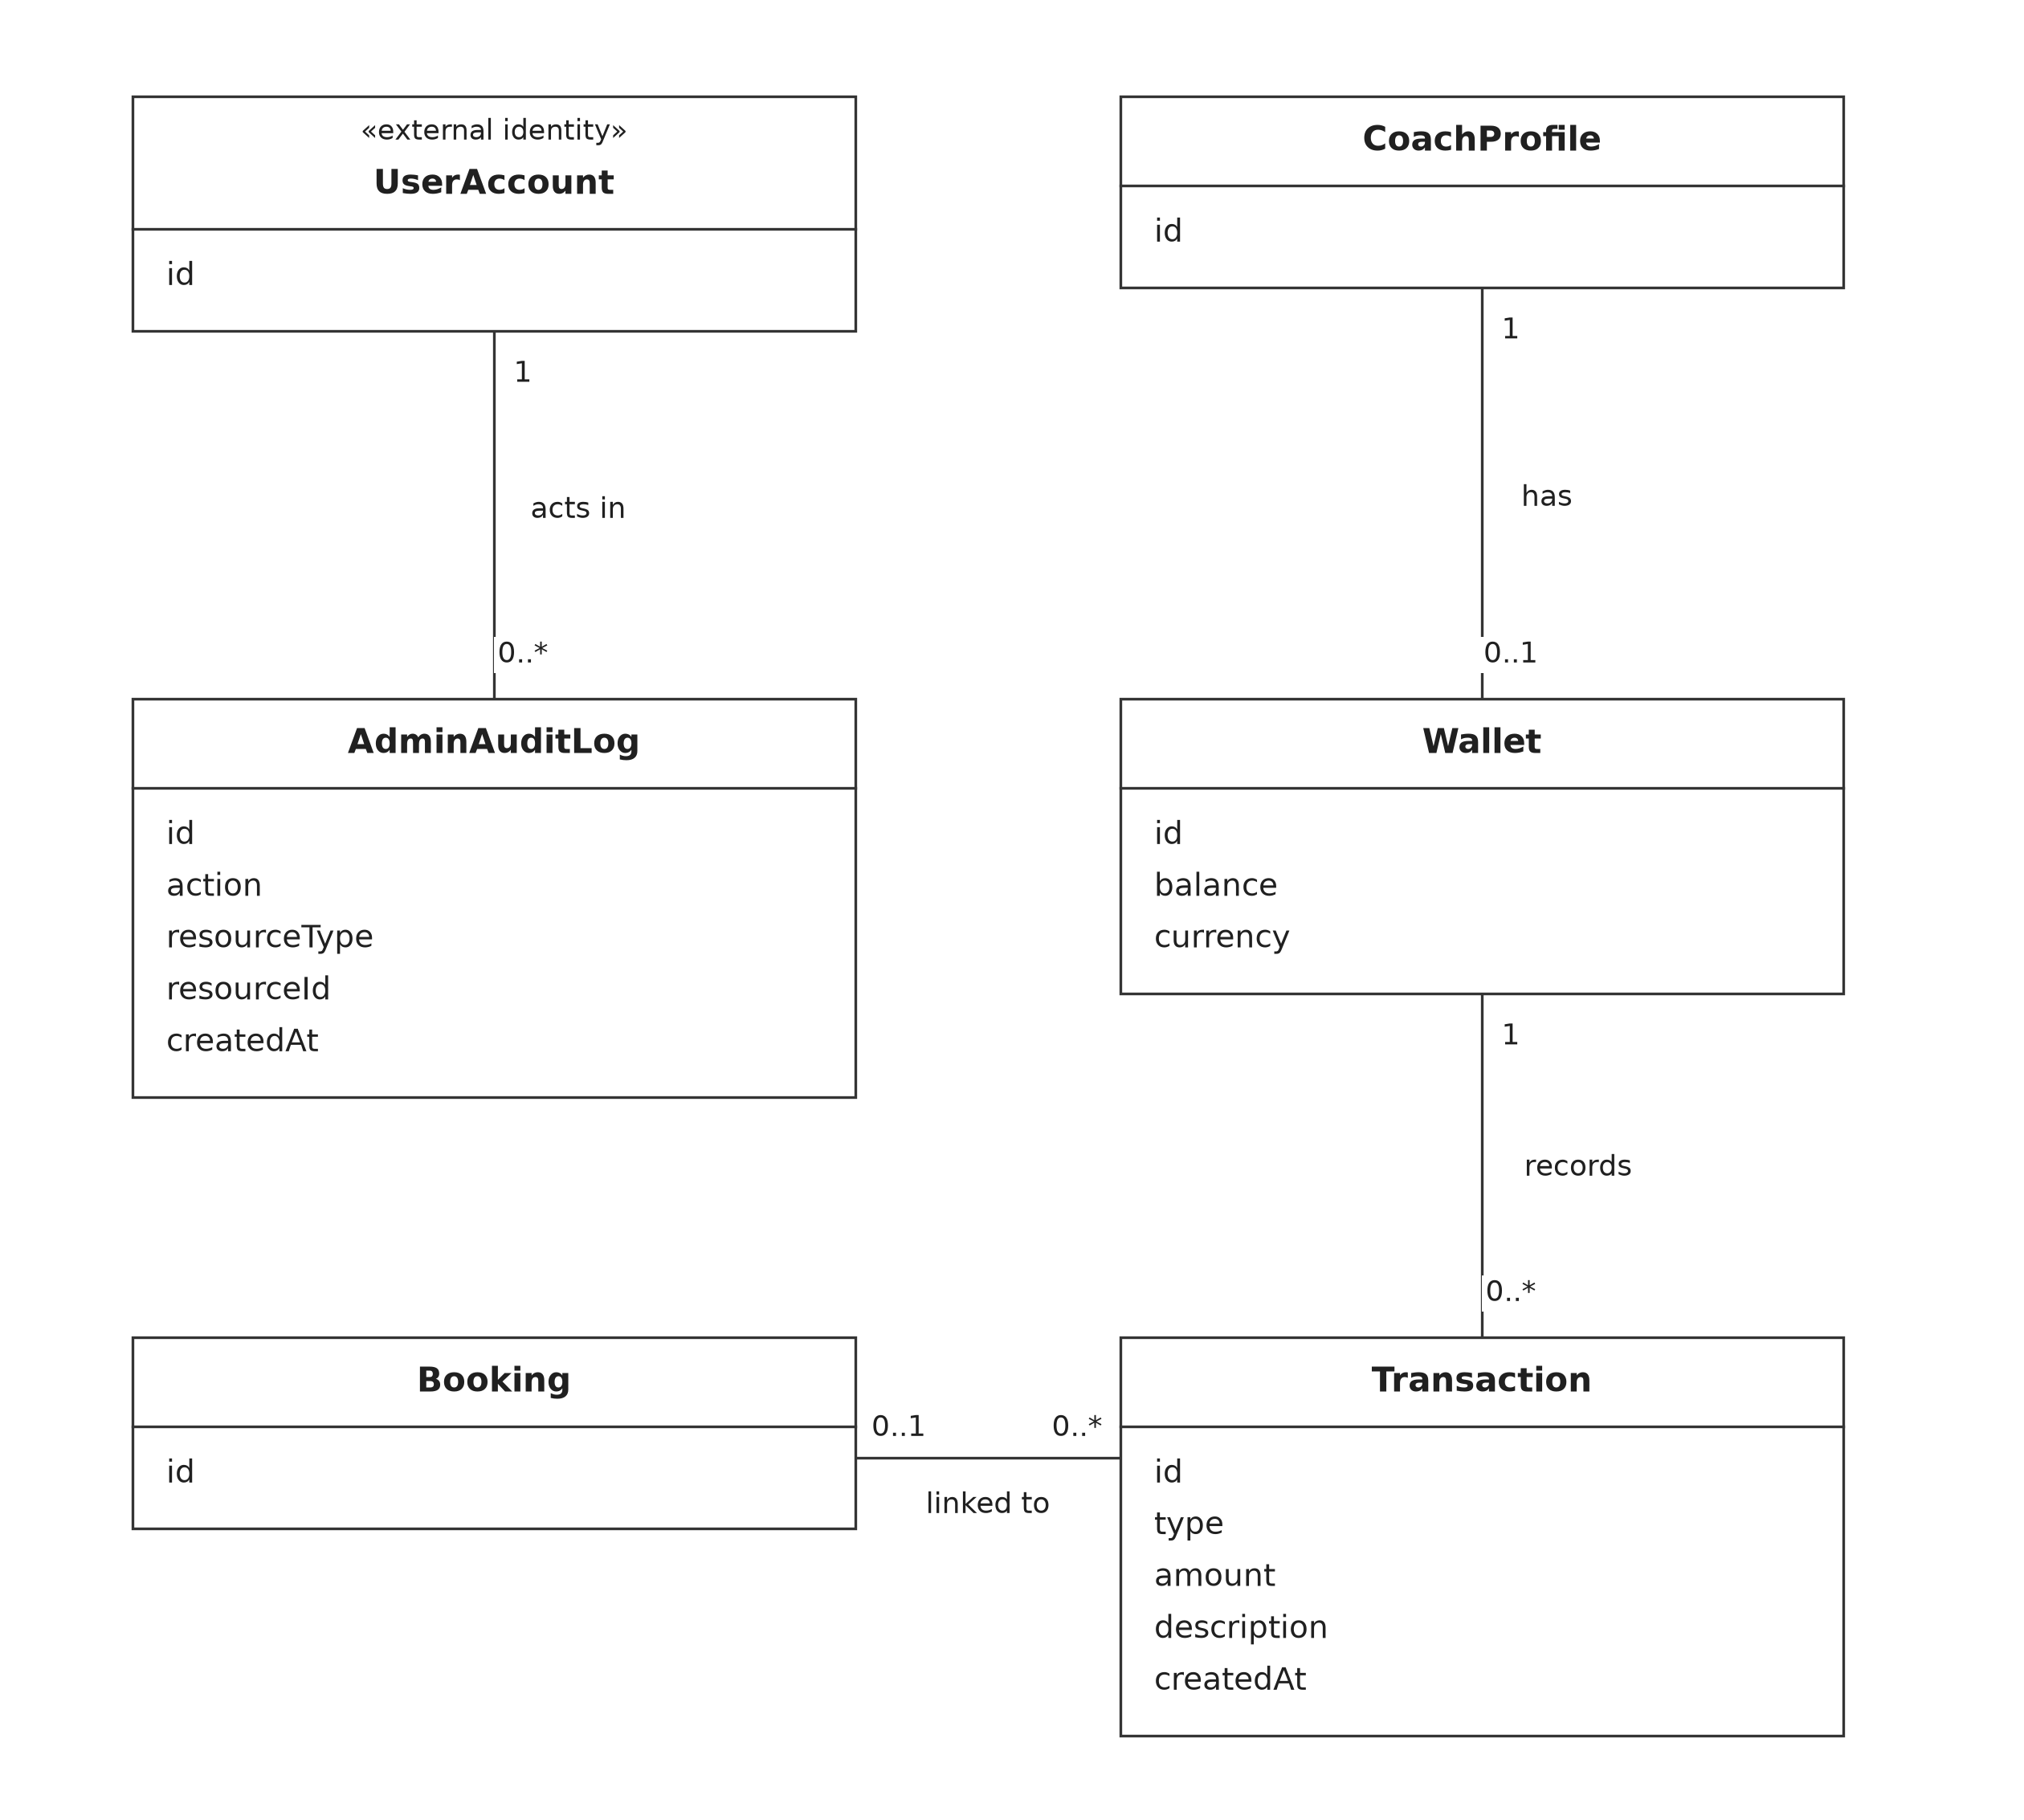
\includegraphics[width=0.95\linewidth]{figures/class_diagram_sprint3_finance.png}
\caption{Sprint 3 cumulative domain model: finance and administration}
\label{fig:class_sprint3_finance}
\end{figure}

\section{Functional Specification of Requirements}

This section specifies the sprint use cases and analyzes the behavioral interactions between the participating actors and the GoFit platform.


\subsection{Refined Use Case Diagram of Sprint 3}

The actors are Client, Coach, and Administrator. The upper view presents client and coach activities: discovery, session-pack purchases, bookings, assigned programs, check-ins, coach-profile completion, availability, client and program management, and coach-facing AI briefings. Messaging and video calls are shared by Client and Coach; the AI briefing is associated only with Coach. The lower view presents account management, coach-profile approval, catalog maintenance, and report review by the Administrator. Both views concern the same GoFit system and are separated for readability. Authentication is a precondition for protected activities, as summarized in the global diagram. These associations identify functional participation; payment settlement, video-call reliability, and approval side effects require the more detailed evidence discussed in the sequence analysis and validation sections.


\begin{figure}[H]
\centering
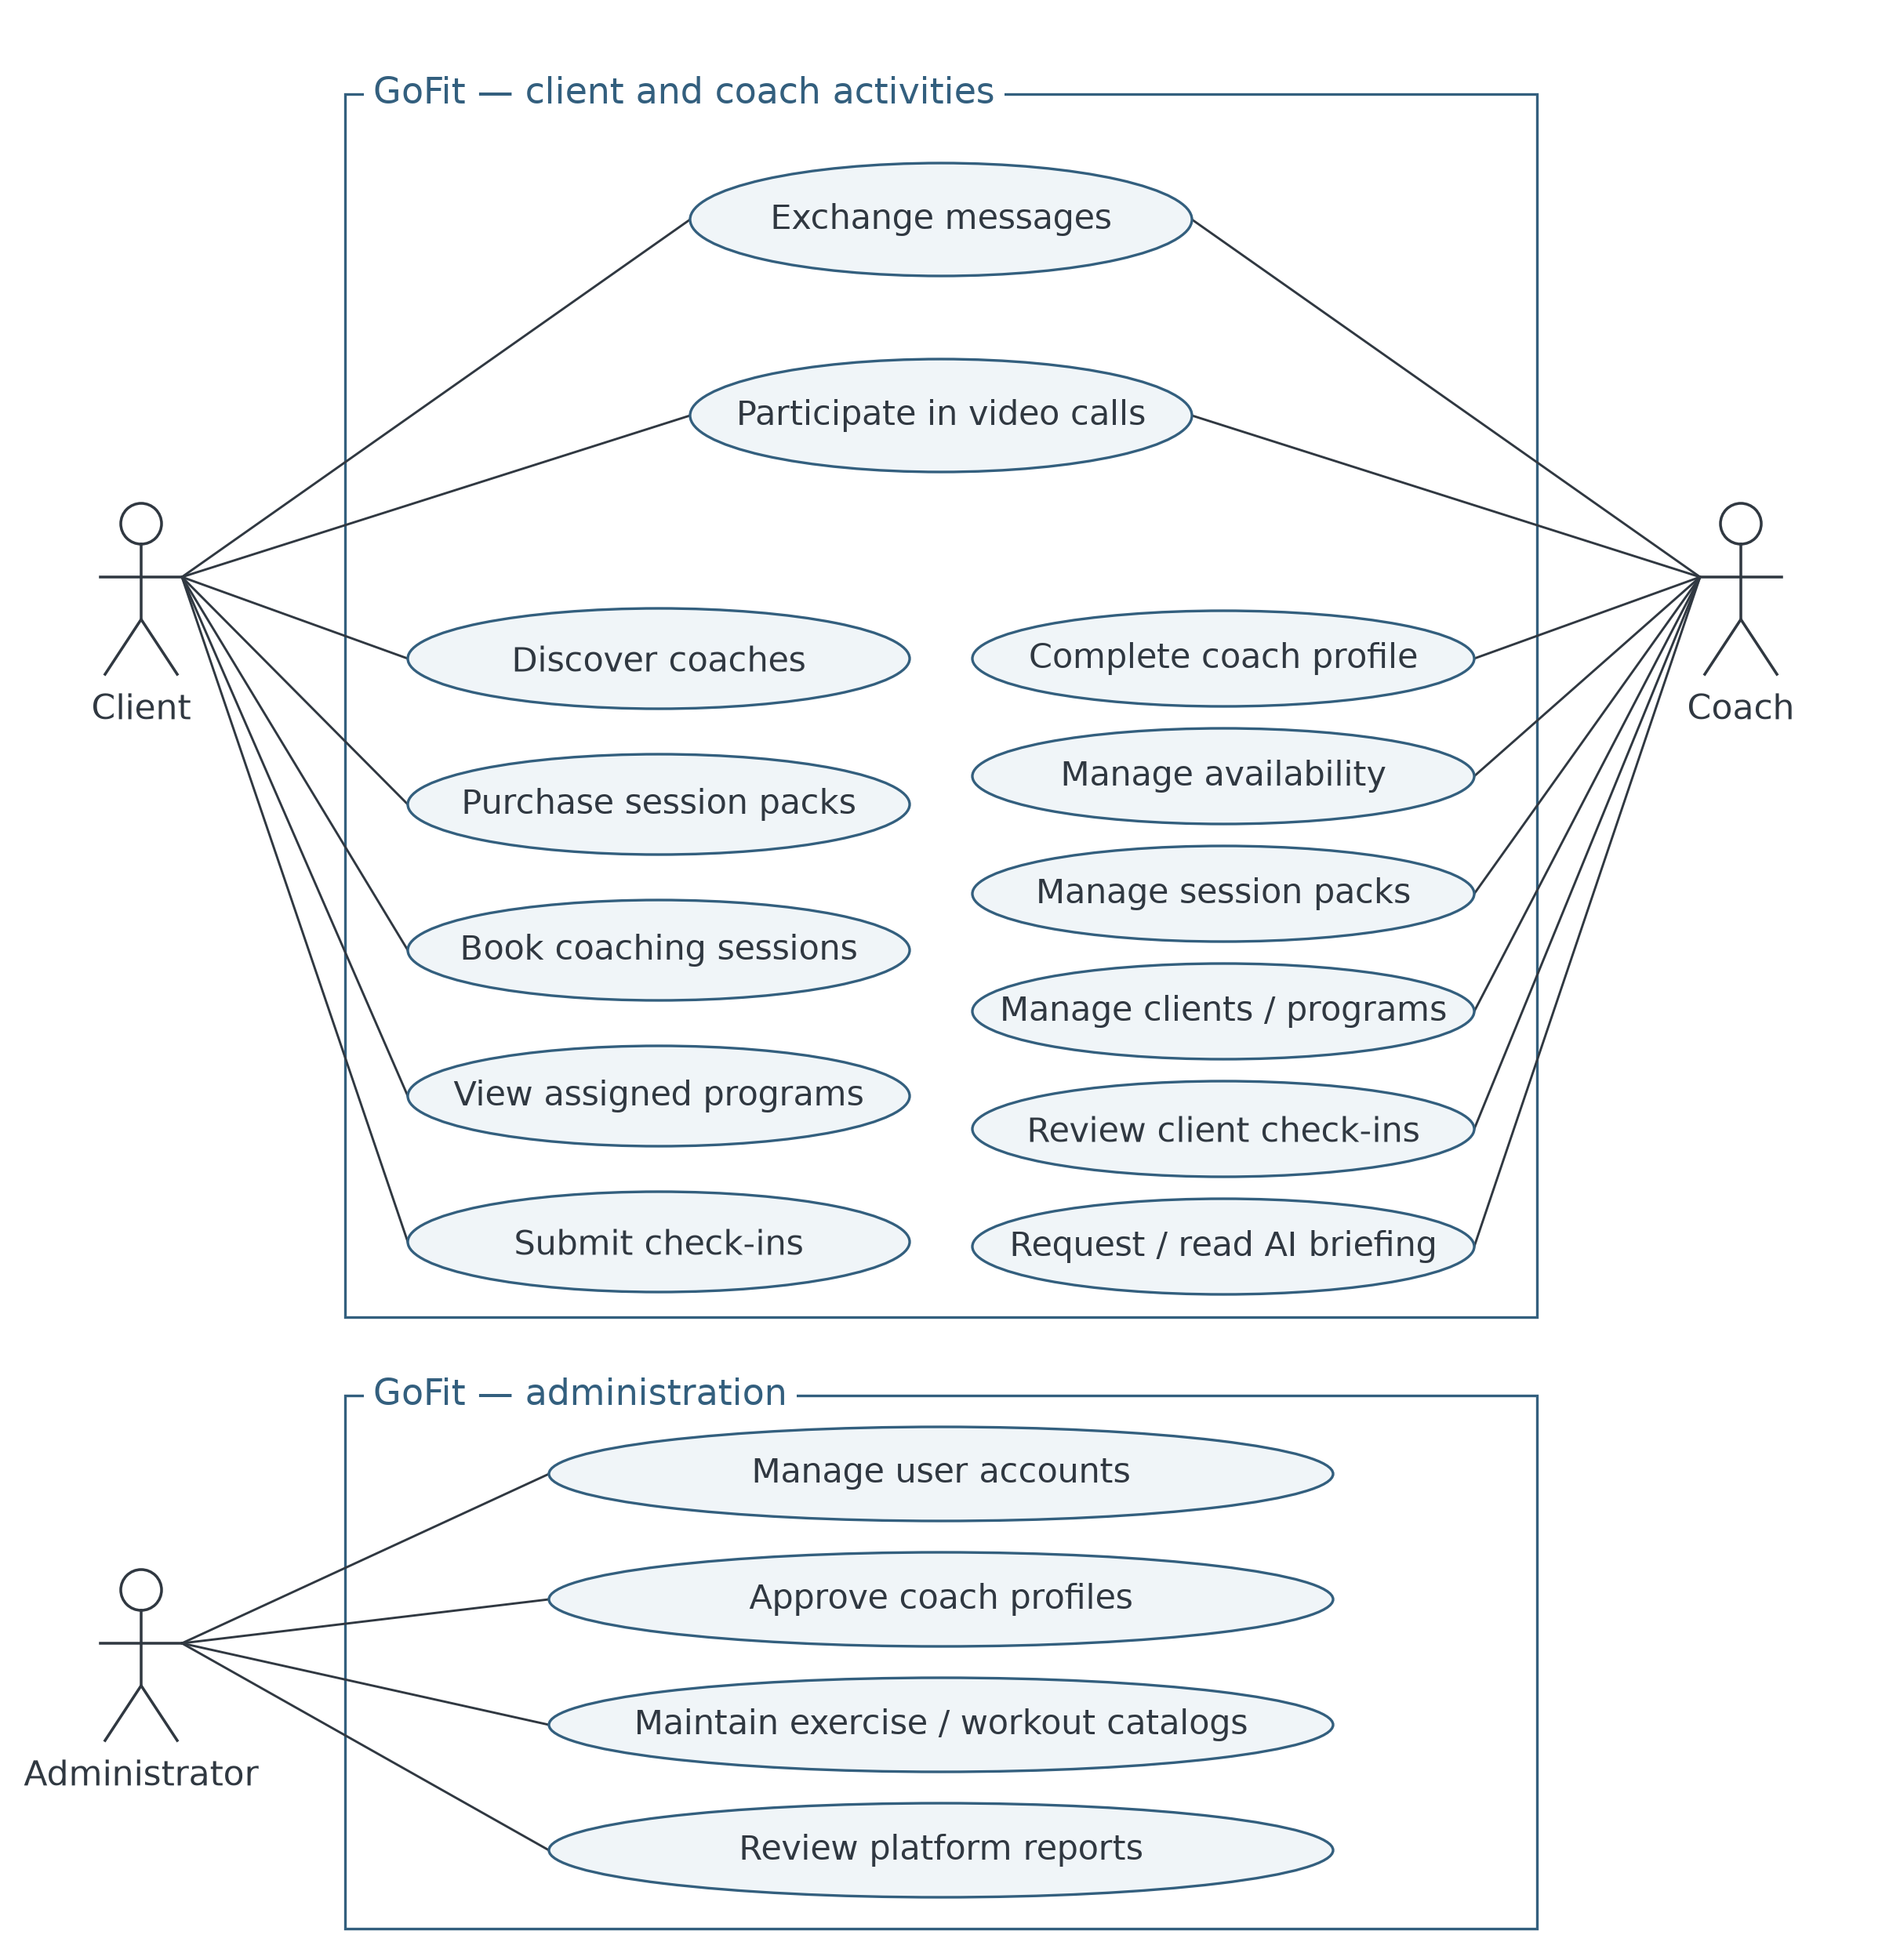
\includegraphics[width=0.92\linewidth]{figures/use_case_sprint3.png}
\caption{Selected Sprint 3 use cases: client and coach activities, and administration}
\label{fig:use_case_sprint3}
\end{figure}

\subsection{Use Case Analysis}

\subsubsection{Use case: Purchase a session pack or pay for a direct booking}

The following use case and sequences describe the corrected implementation inspected on 24 October 2026. They replace the earlier client-priced USD checkout baseline and must not be read as evidence of internship-period delivery. Pack purchase and standalone session payment share native PaymentSheet presentation but have different reservation and fulfilment paths. Section~\ref{sec:current-payment-boundaries} distinguishes the retained Android pack evidence from standalone API/provider checks and outstanding native verification.

\begingroup
\footnotesize
\setlength{\tabcolsep}{3pt}
\renewcommand{\arraystretch}{1.20}
\setlength{\LTpre}{5pt}
\setlength{\LTpost}{10pt}
\begin{longtable}{|L{4.95cm}|L{10.05cm}|}
\caption{Textual description of use case: Purchase a session pack or pay for a direct booking}\label{tab:pdf-71-32} \\
\hline
\rowcolor{entetetab}
Field & Description \\ \hline
\endfirsthead
\hline
\rowcolor{entetetab}
Field & Description \\ \hline
\endhead
Use case & Purchase a session pack or pay for a direct booking \\ \hline
Primary actor & Mobile user (Client) \\ \hline
Preconditions & The client is authenticated, a coach and pack or session time have been selected, and Stripe client/server configuration is available. A standalone session requires an approved coach, a positive hourly rate, the saved duration and a valid Europe/Berlin availability slot. \\ \hline
Postconditions & On verified pack fulfilment, one purchased-pack record retains the payment reference, paid EUR amount, mode and credits. On verified standalone fulfilment, the reserved booking is confirmed and marked paid after capture. Provider success and database confirmation are separate boundaries; recovery may still require retrying the same reference. \\ \hline
Nominal scenario & 1. The client opens the coach profile. 2. The client selects a pack or a standalone session time. 3. The screen requests create\_pack or create\_session. 4. The server authenticates the caller and resolves the EUR price; the session branch first reserves the slot. 5. The screen presents PaymentSheet. 6. After a result without an error, it requests server fulfilment using the PaymentIntent reference. 7. The server verifies ownership and provider state, persists the purchase or captures and confirms the reserved session. 8. The screen displays success only after fulfilment returns successfully. \\ \hline
Alternative scenario & 2.1. Pack checkout uses the active offer price and does not reserve a time. 2.2. Standalone pricing uses hourly rate multiplied by the saved duration divided by 60; the submitted expected amount is checked against the server quote. The card is authorized before capture. 6.1. A fulfilment replay returns the existing result without granting duplicate credits or recapturing a paid session. Pack-credit redemption remains a separate service branch, not the standalone checkout shown here. \\ \hline
Exception scenario & E.1. Missing configuration, changed terms, unavailable time or reservation conflict prevents checkout. E.2. A cancelled or failed native sheet does not initiate fulfilment; the session screen attempts checkout cancellation. E.3. Expired or cancelled session reservations cannot proceed to capture. E.4. Provider success followed by a persistence failure requires retry with the same reference; no webhook, automatic refund or app-restart recovery is established. E.5. A capture in progress cannot be cancelled by the checkout-cancellation operation. \\ \hline
\end{longtable}
\endgroup

\begin{figure}[H]
\centering
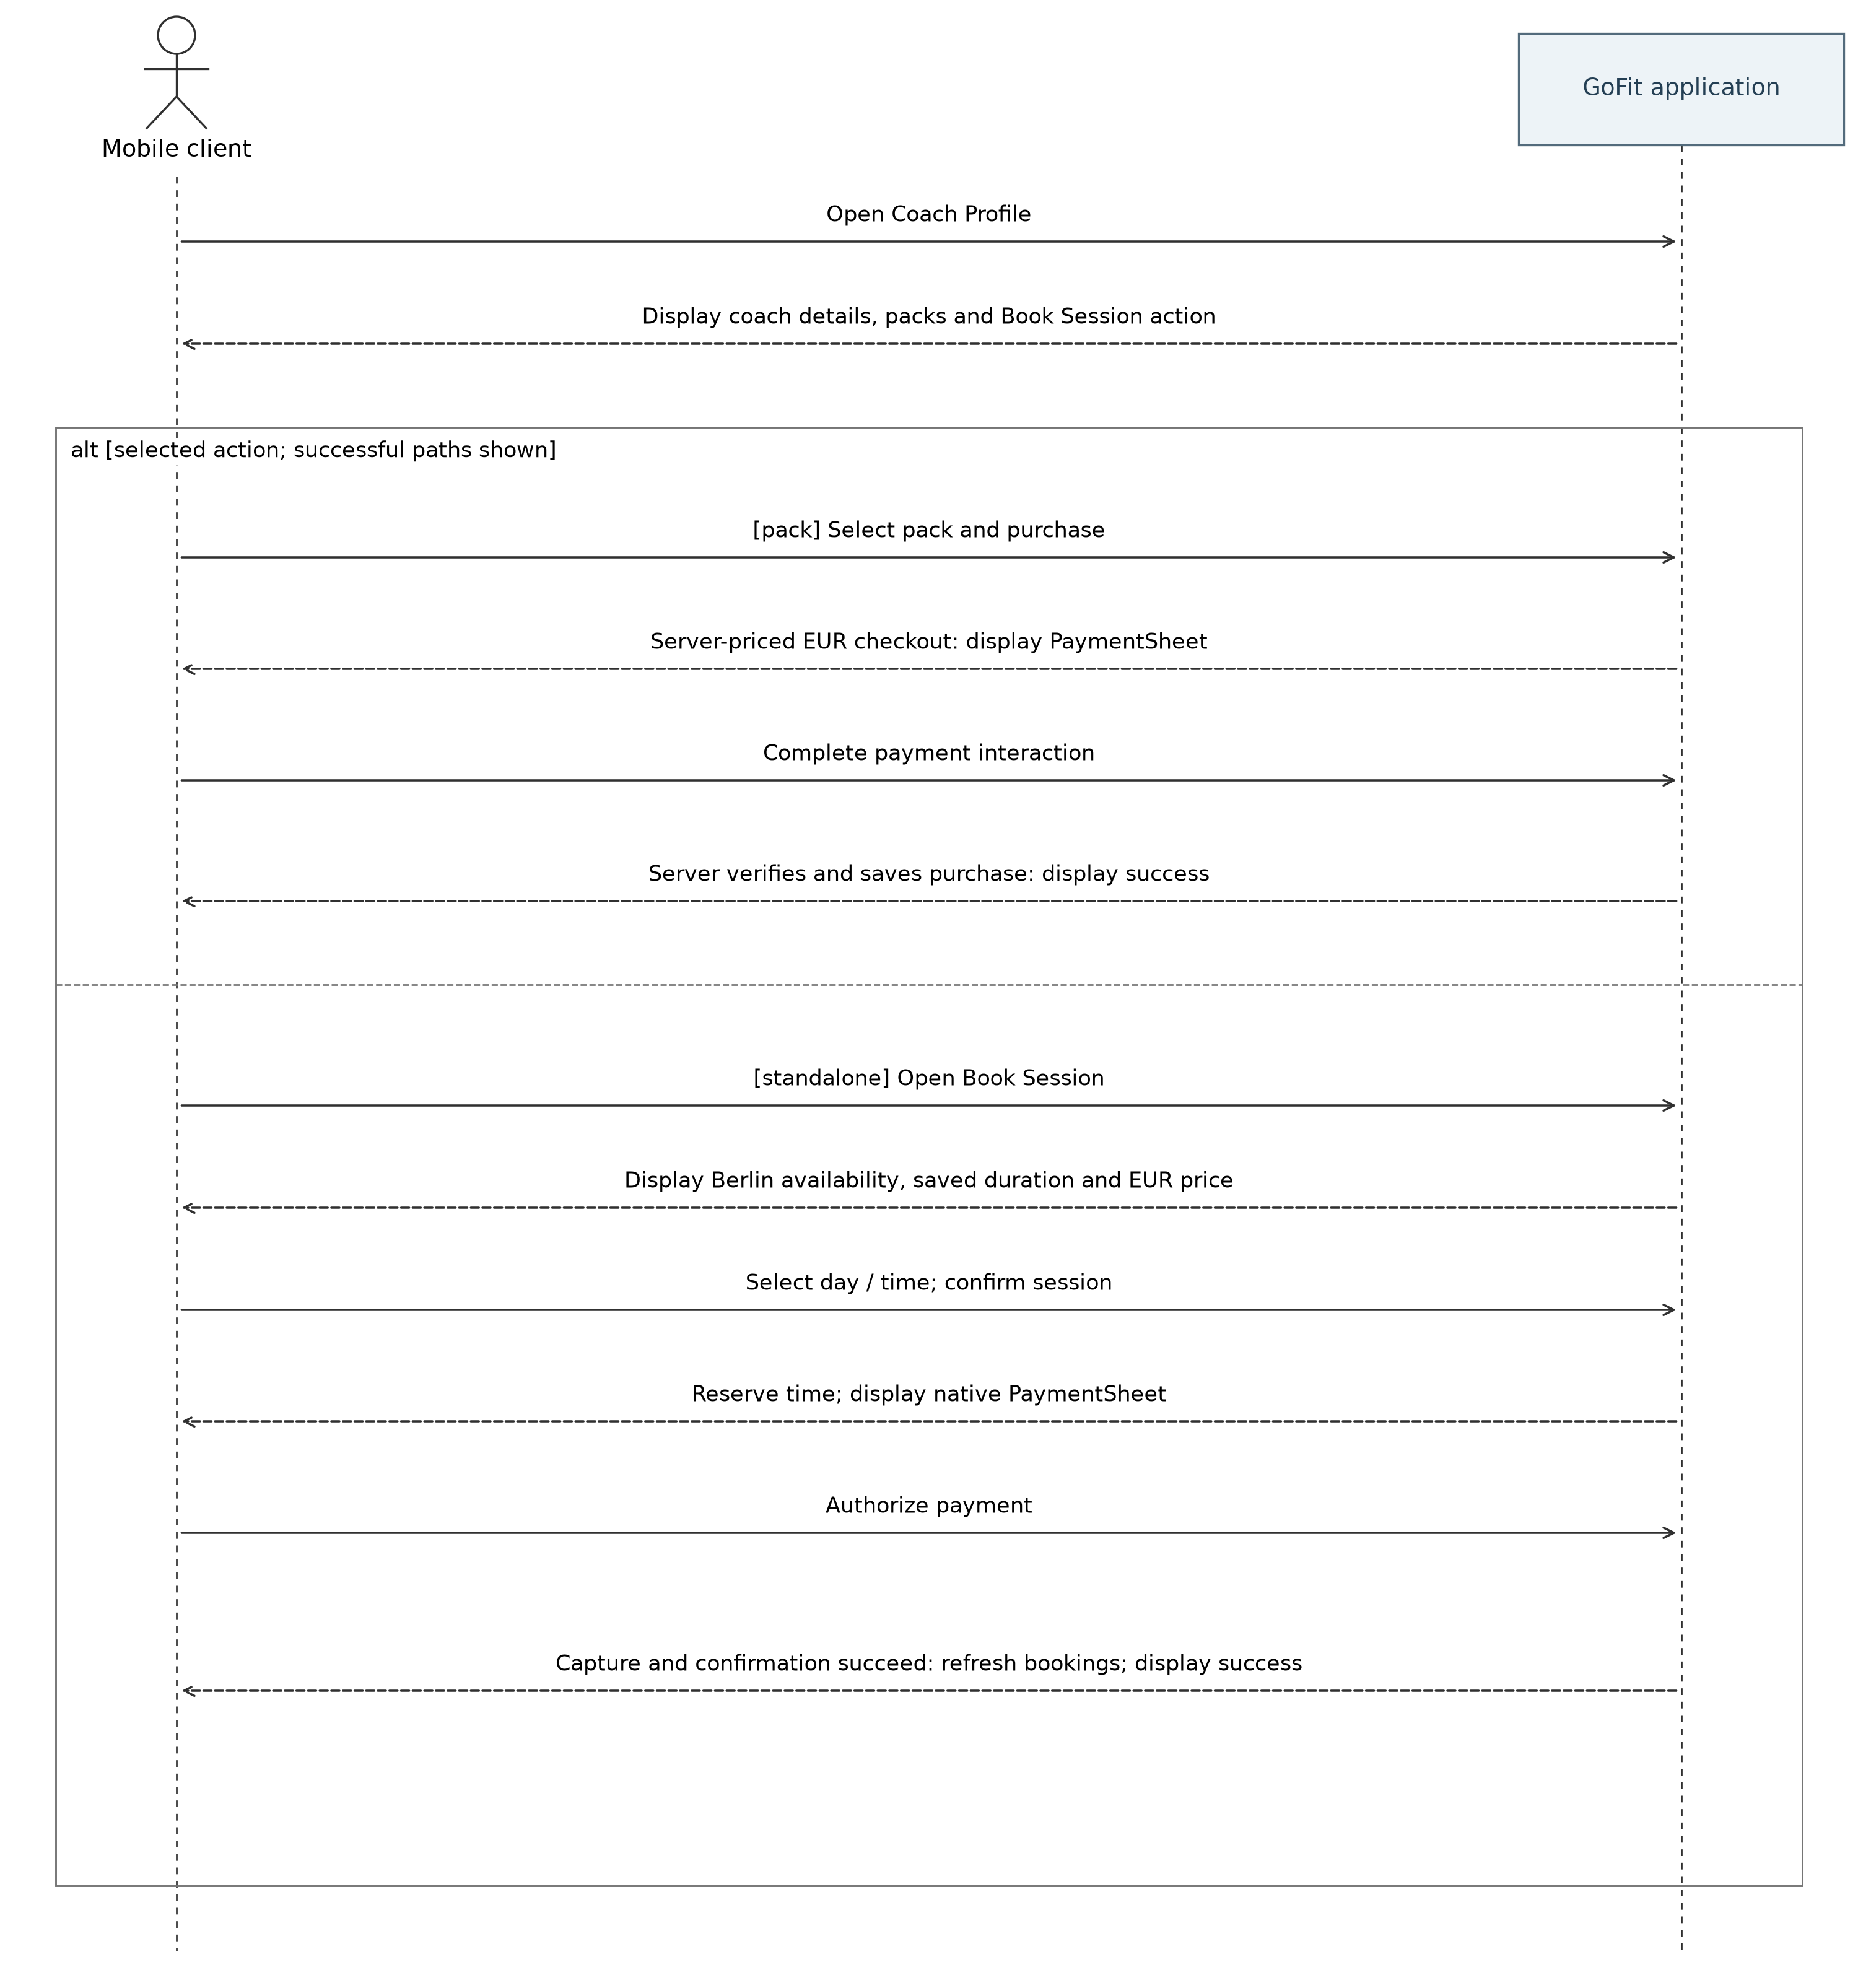
\includegraphics[width=0.92\linewidth]{figures/seq_booking_ssd.png}
\caption{System sequence diagram: Alternative pack purchase and direct-booking journeys}
\label{fig:seq_booking_ssd}
\end{figure}

\begin{figure}[H]
\centering
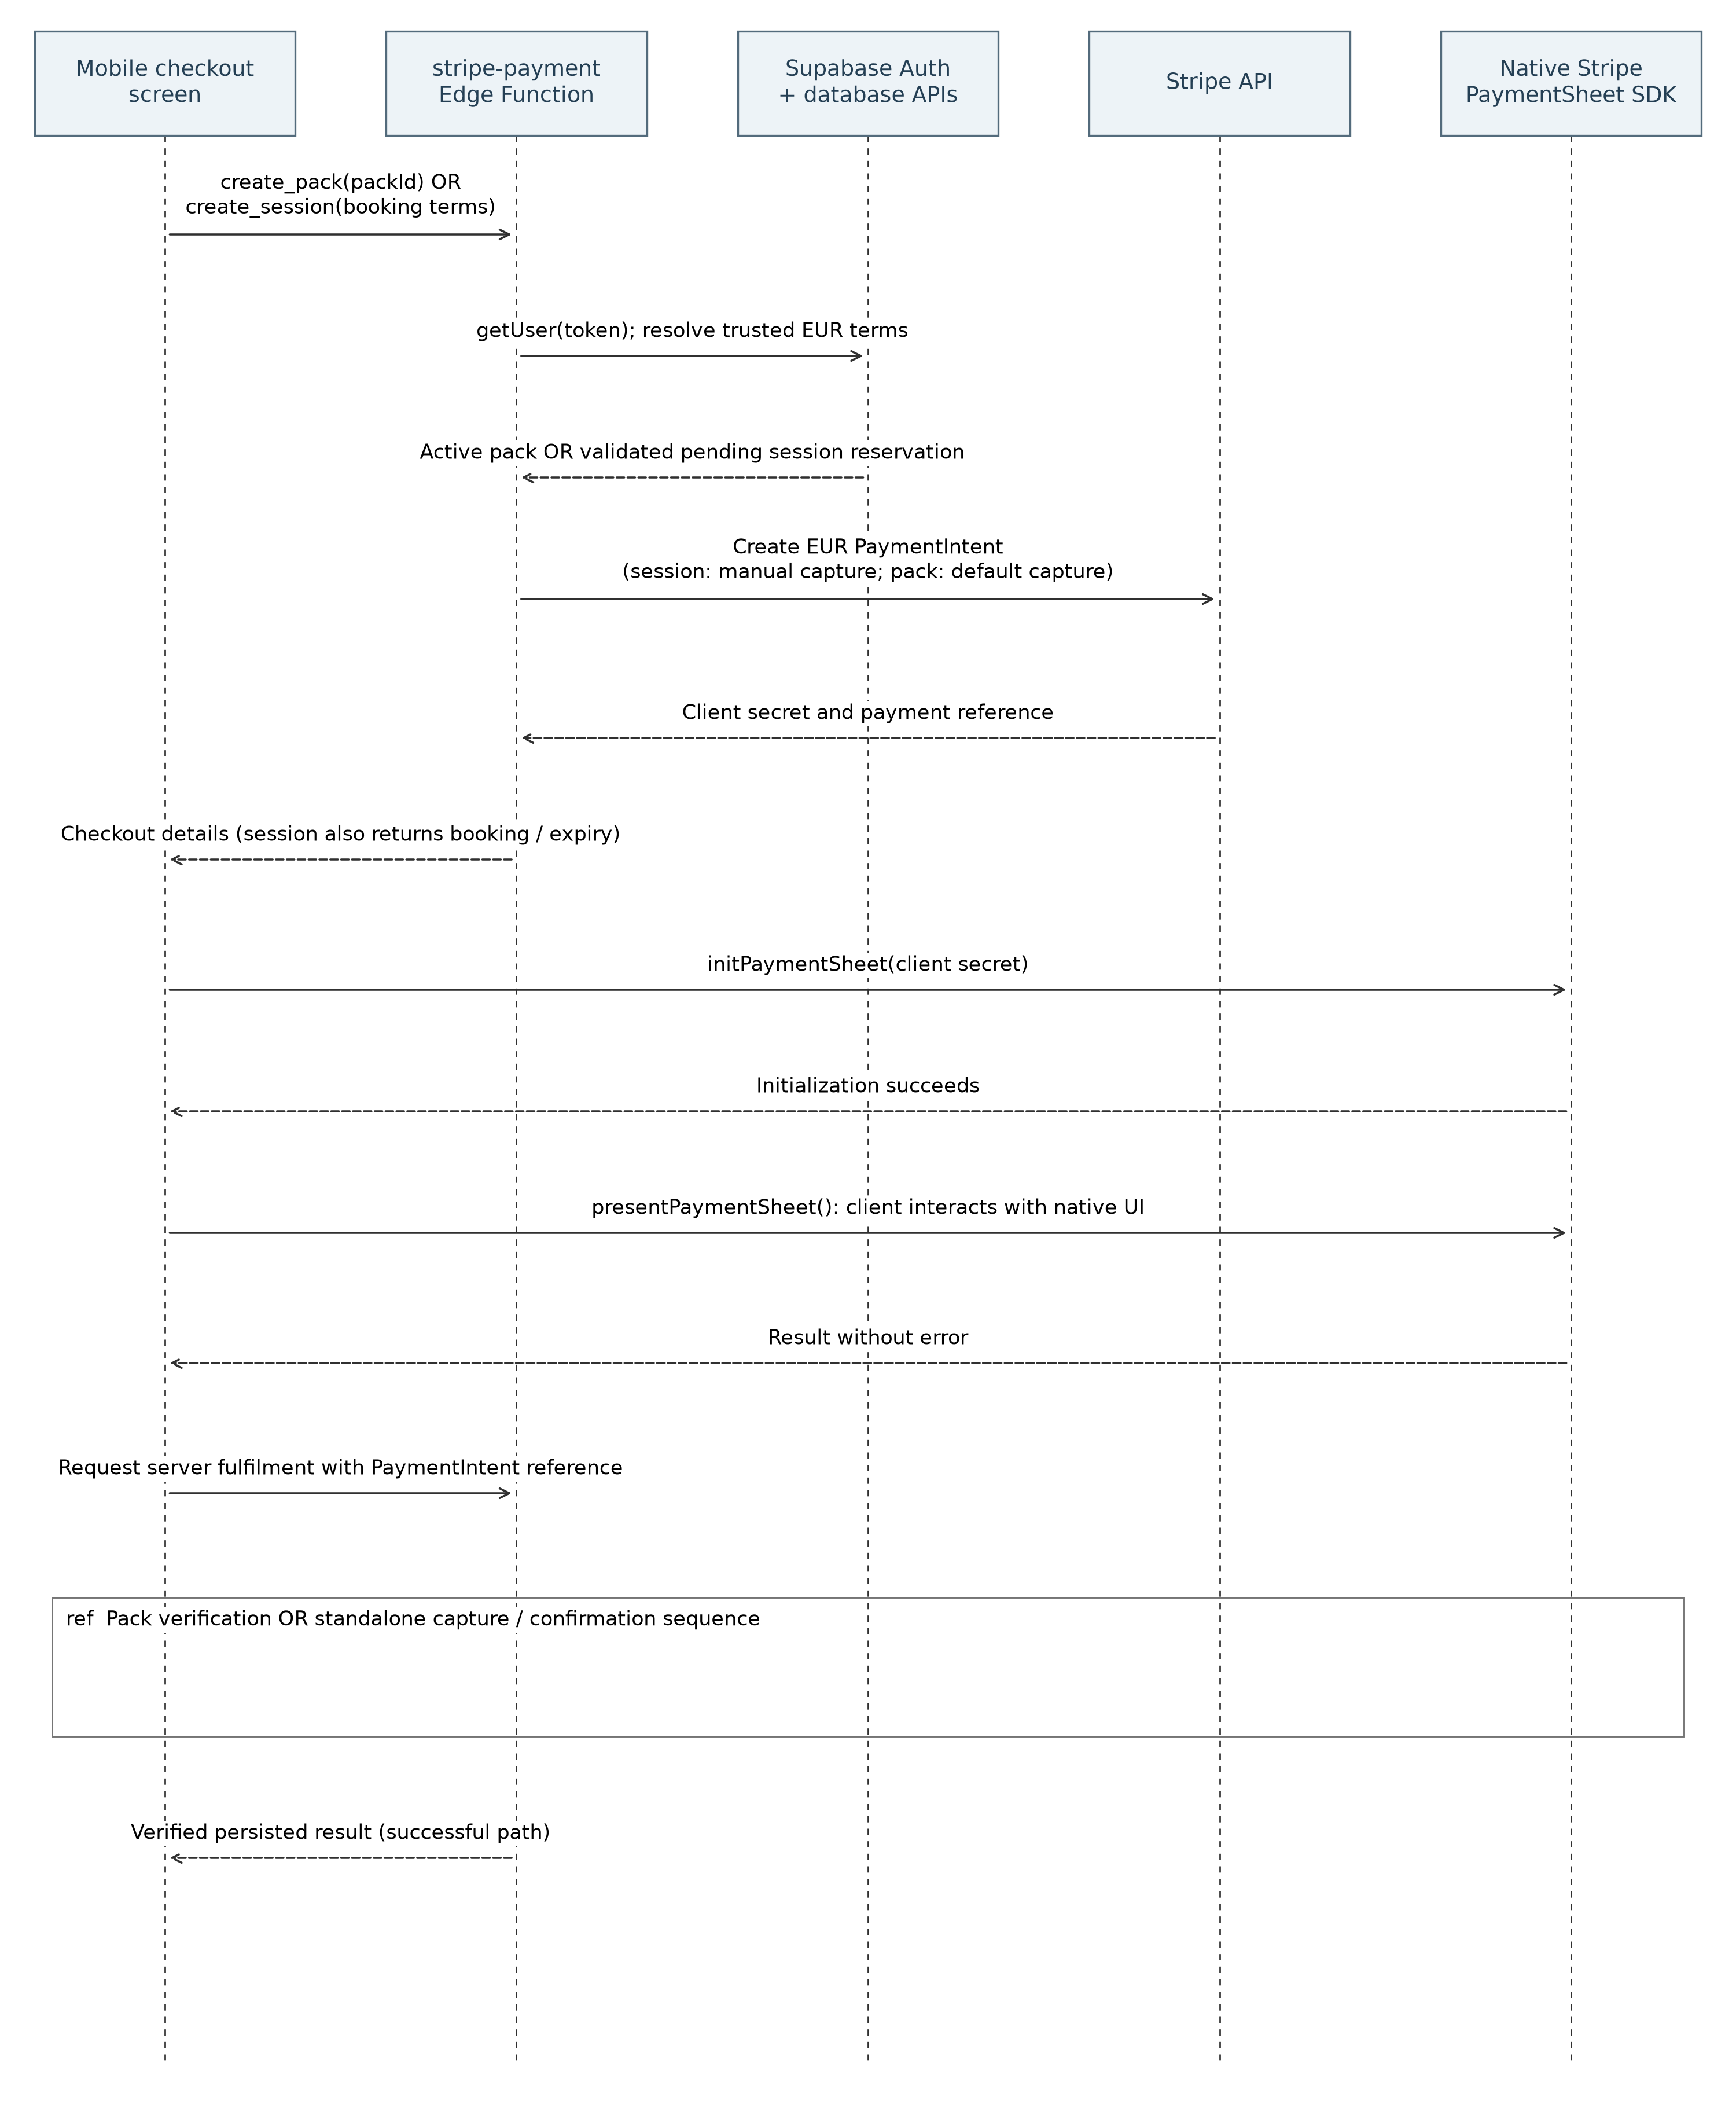
\includegraphics[width=0.92\linewidth]{figures/seq_booking_detailed.png}
\caption{Technical sequence diagram: Server-priced EUR initialization and native checkout}
\label{fig:seq_booking_detailed}
\end{figure}

Figure~\ref{fig:seq_booking_ssd} makes the client journey explicit: Coach Profile leads either to a pack purchase or to Book Session, availability selection and standalone checkout. A pack purchase does not itself book a time. The standalone screen loads saved duration, price and busy slots, then rechecks terms before requesting a reservation. The date helper interprets availability in Europe/Berlin and chooses the next occurrence of the selected weekday, including the following week when that weekday is today. Sunday is accepted through an explicit null check. Client-side filtering assists selection; the server remains responsible for reservation and conflict checks.

Figure~\ref{fig:seq_booking_detailed} separates checkout initialization from fulfilment. The Edge Function validates the supplied session token using the authentication service. Pack initialization resolves an active offer and EUR price; standalone initialization calls \texttt{reserve\_paid\_session}, which validates the coach, saved duration, expected price and availability before inserting a pending reservation. Its checkout expiry is at most 15 minutes and no later than the session start. The session PaymentIntent uses manual capture. The native SDK presents PaymentSheet; a return without error triggers a server request rather than a direct client database insert. The selected successful sequences omit SDK-internal network exchanges and most error branches, which remain in the use-case table. Apple Pay and Google Pay are not configured by these calls.

\begin{figure}[H]
\centering
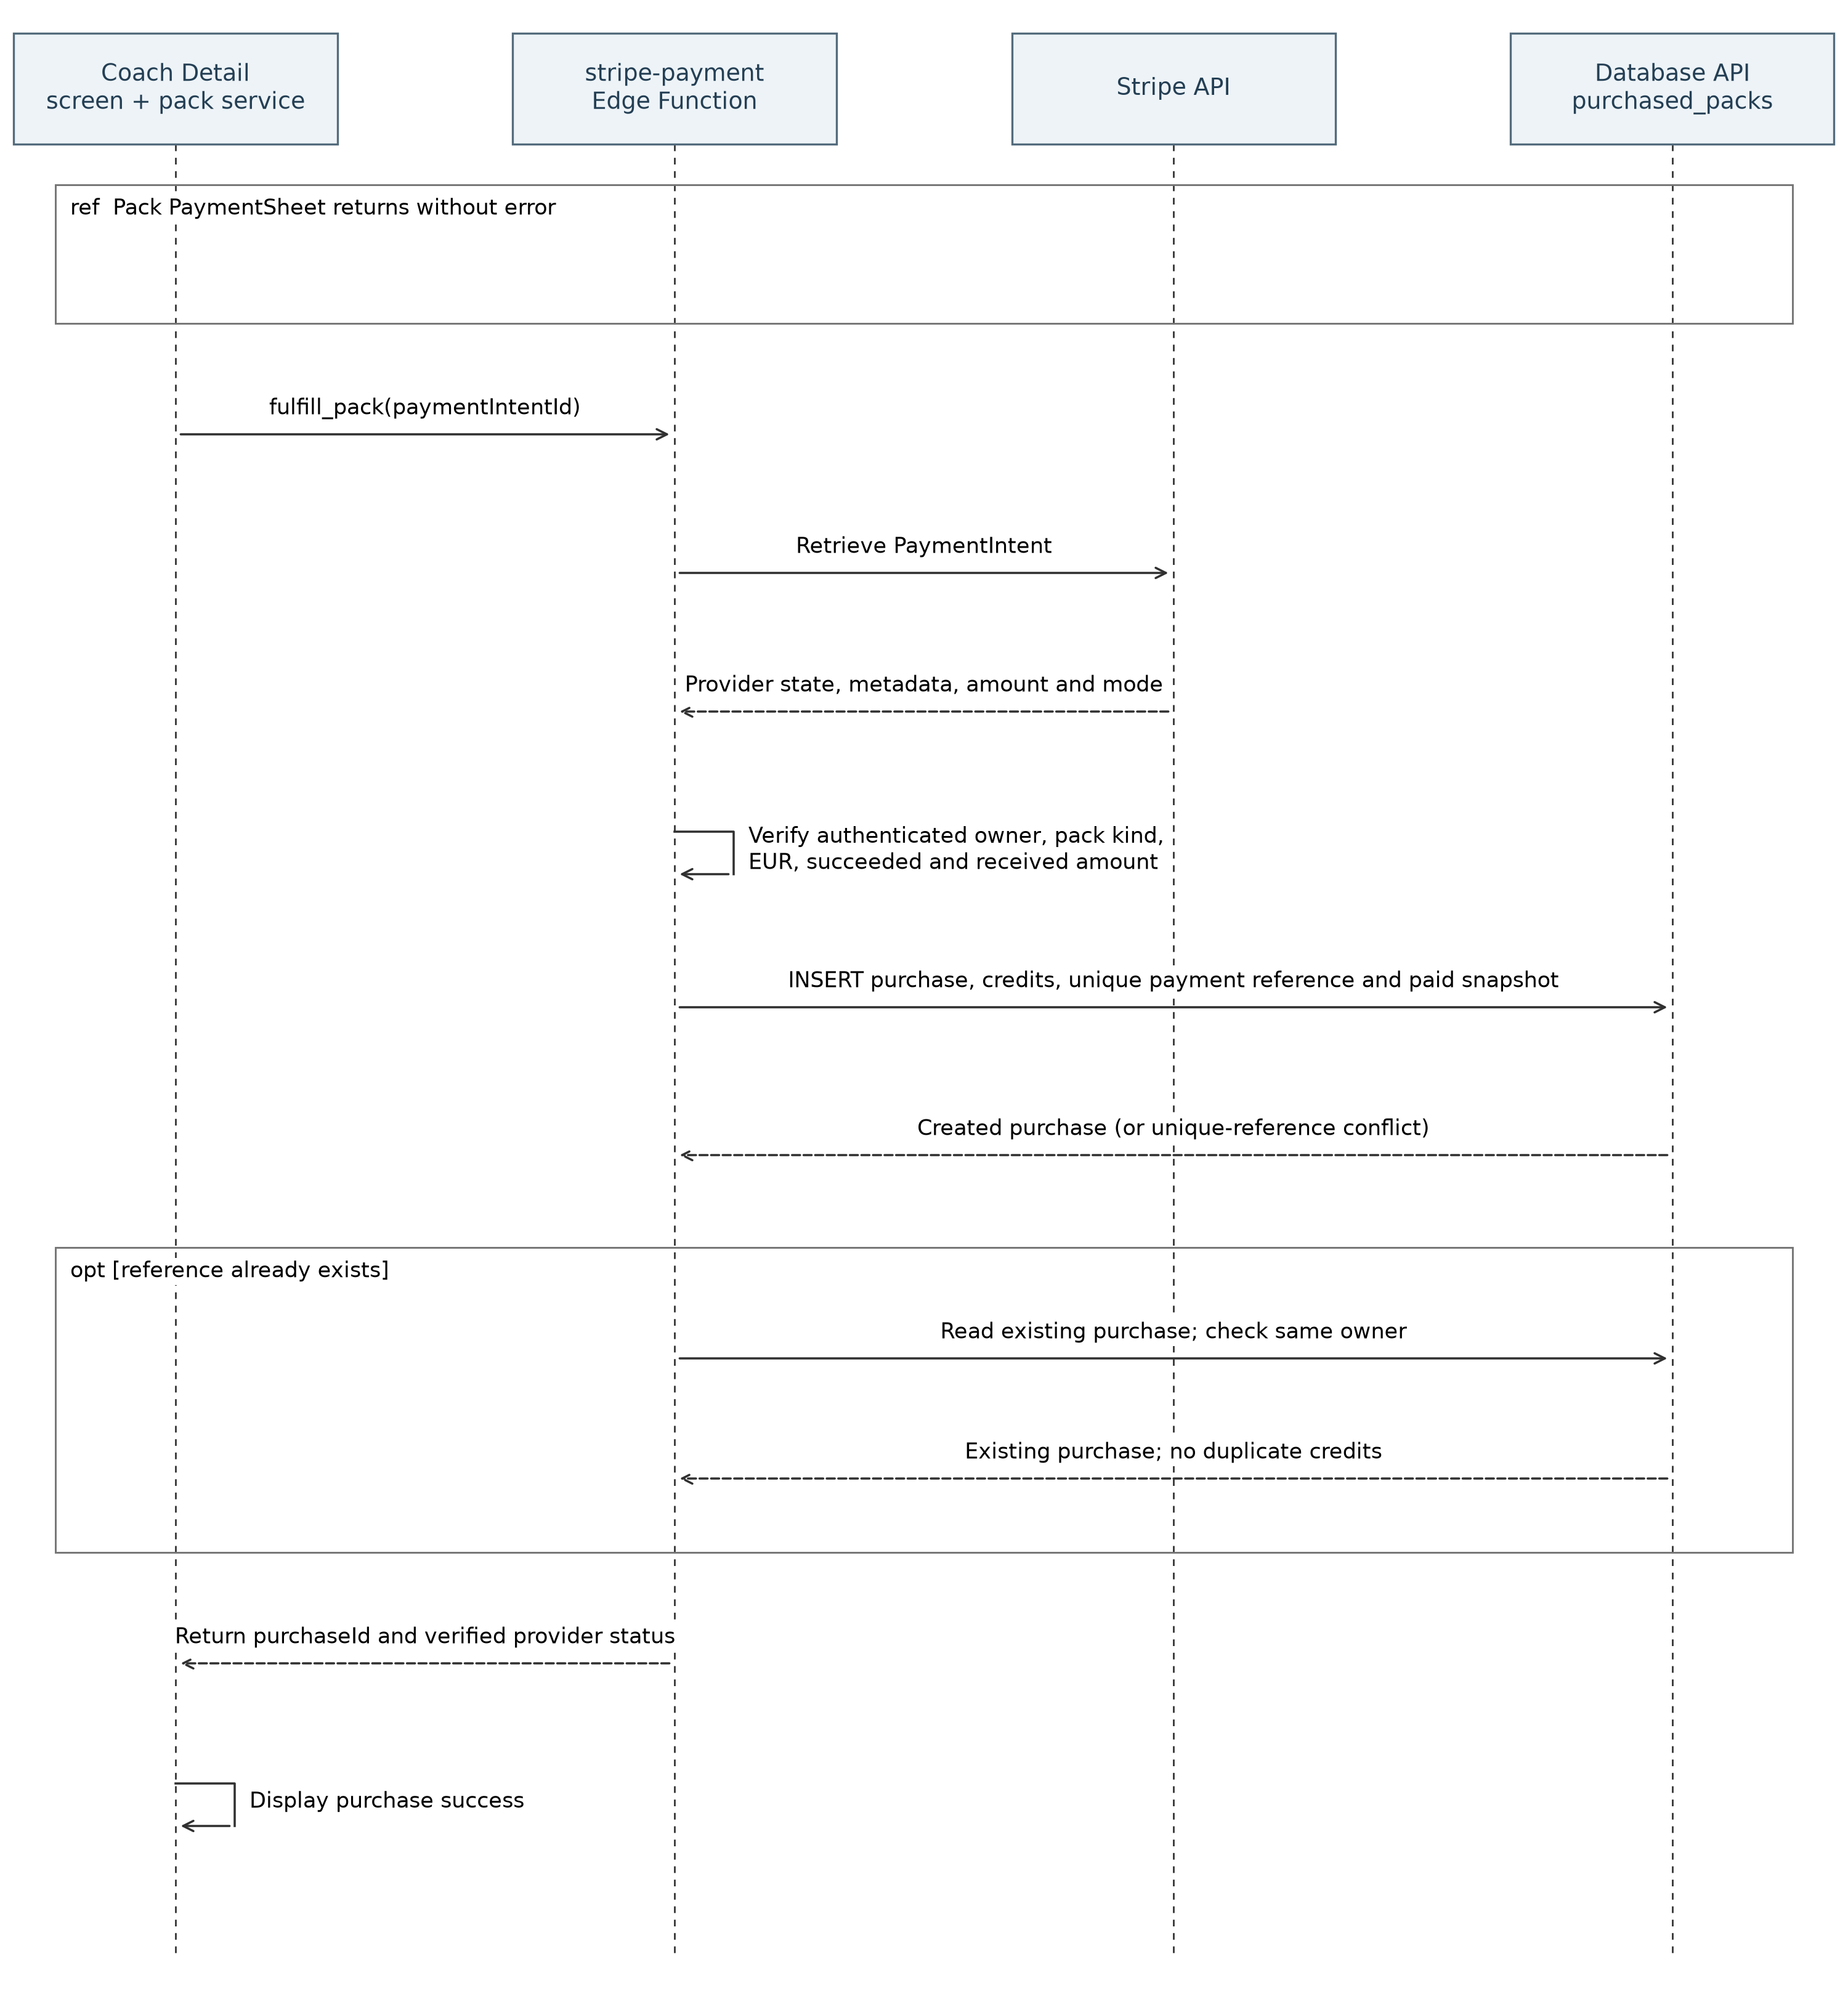
\includegraphics[width=0.95\linewidth]{figures/seq_booking_pack_recording.png}
\caption{Technical sequence diagram: Server verification and idempotent pack fulfilment}
\label{fig:seq_booking_pack_recording}
\end{figure}

Figure~\ref{fig:seq_booking_pack_recording} starts after PaymentSheet returns without an error. The pack service invokes \texttt{fulfill\_pack} with the PaymentIntent reference. The server retrieves the provider record, verifies the authenticated owner, checkout metadata, EUR currency, successful state and received amount, then inserts the purchase with the paid snapshot and credit count. A unique payment reference prevents duplicate credit creation; a matching replay returns the existing purchase. An October Android sandbox purchase and replay support this narrow path, without certifying declines, refunds, payouts or restart recovery.

\begin{figure}[H]
\centering
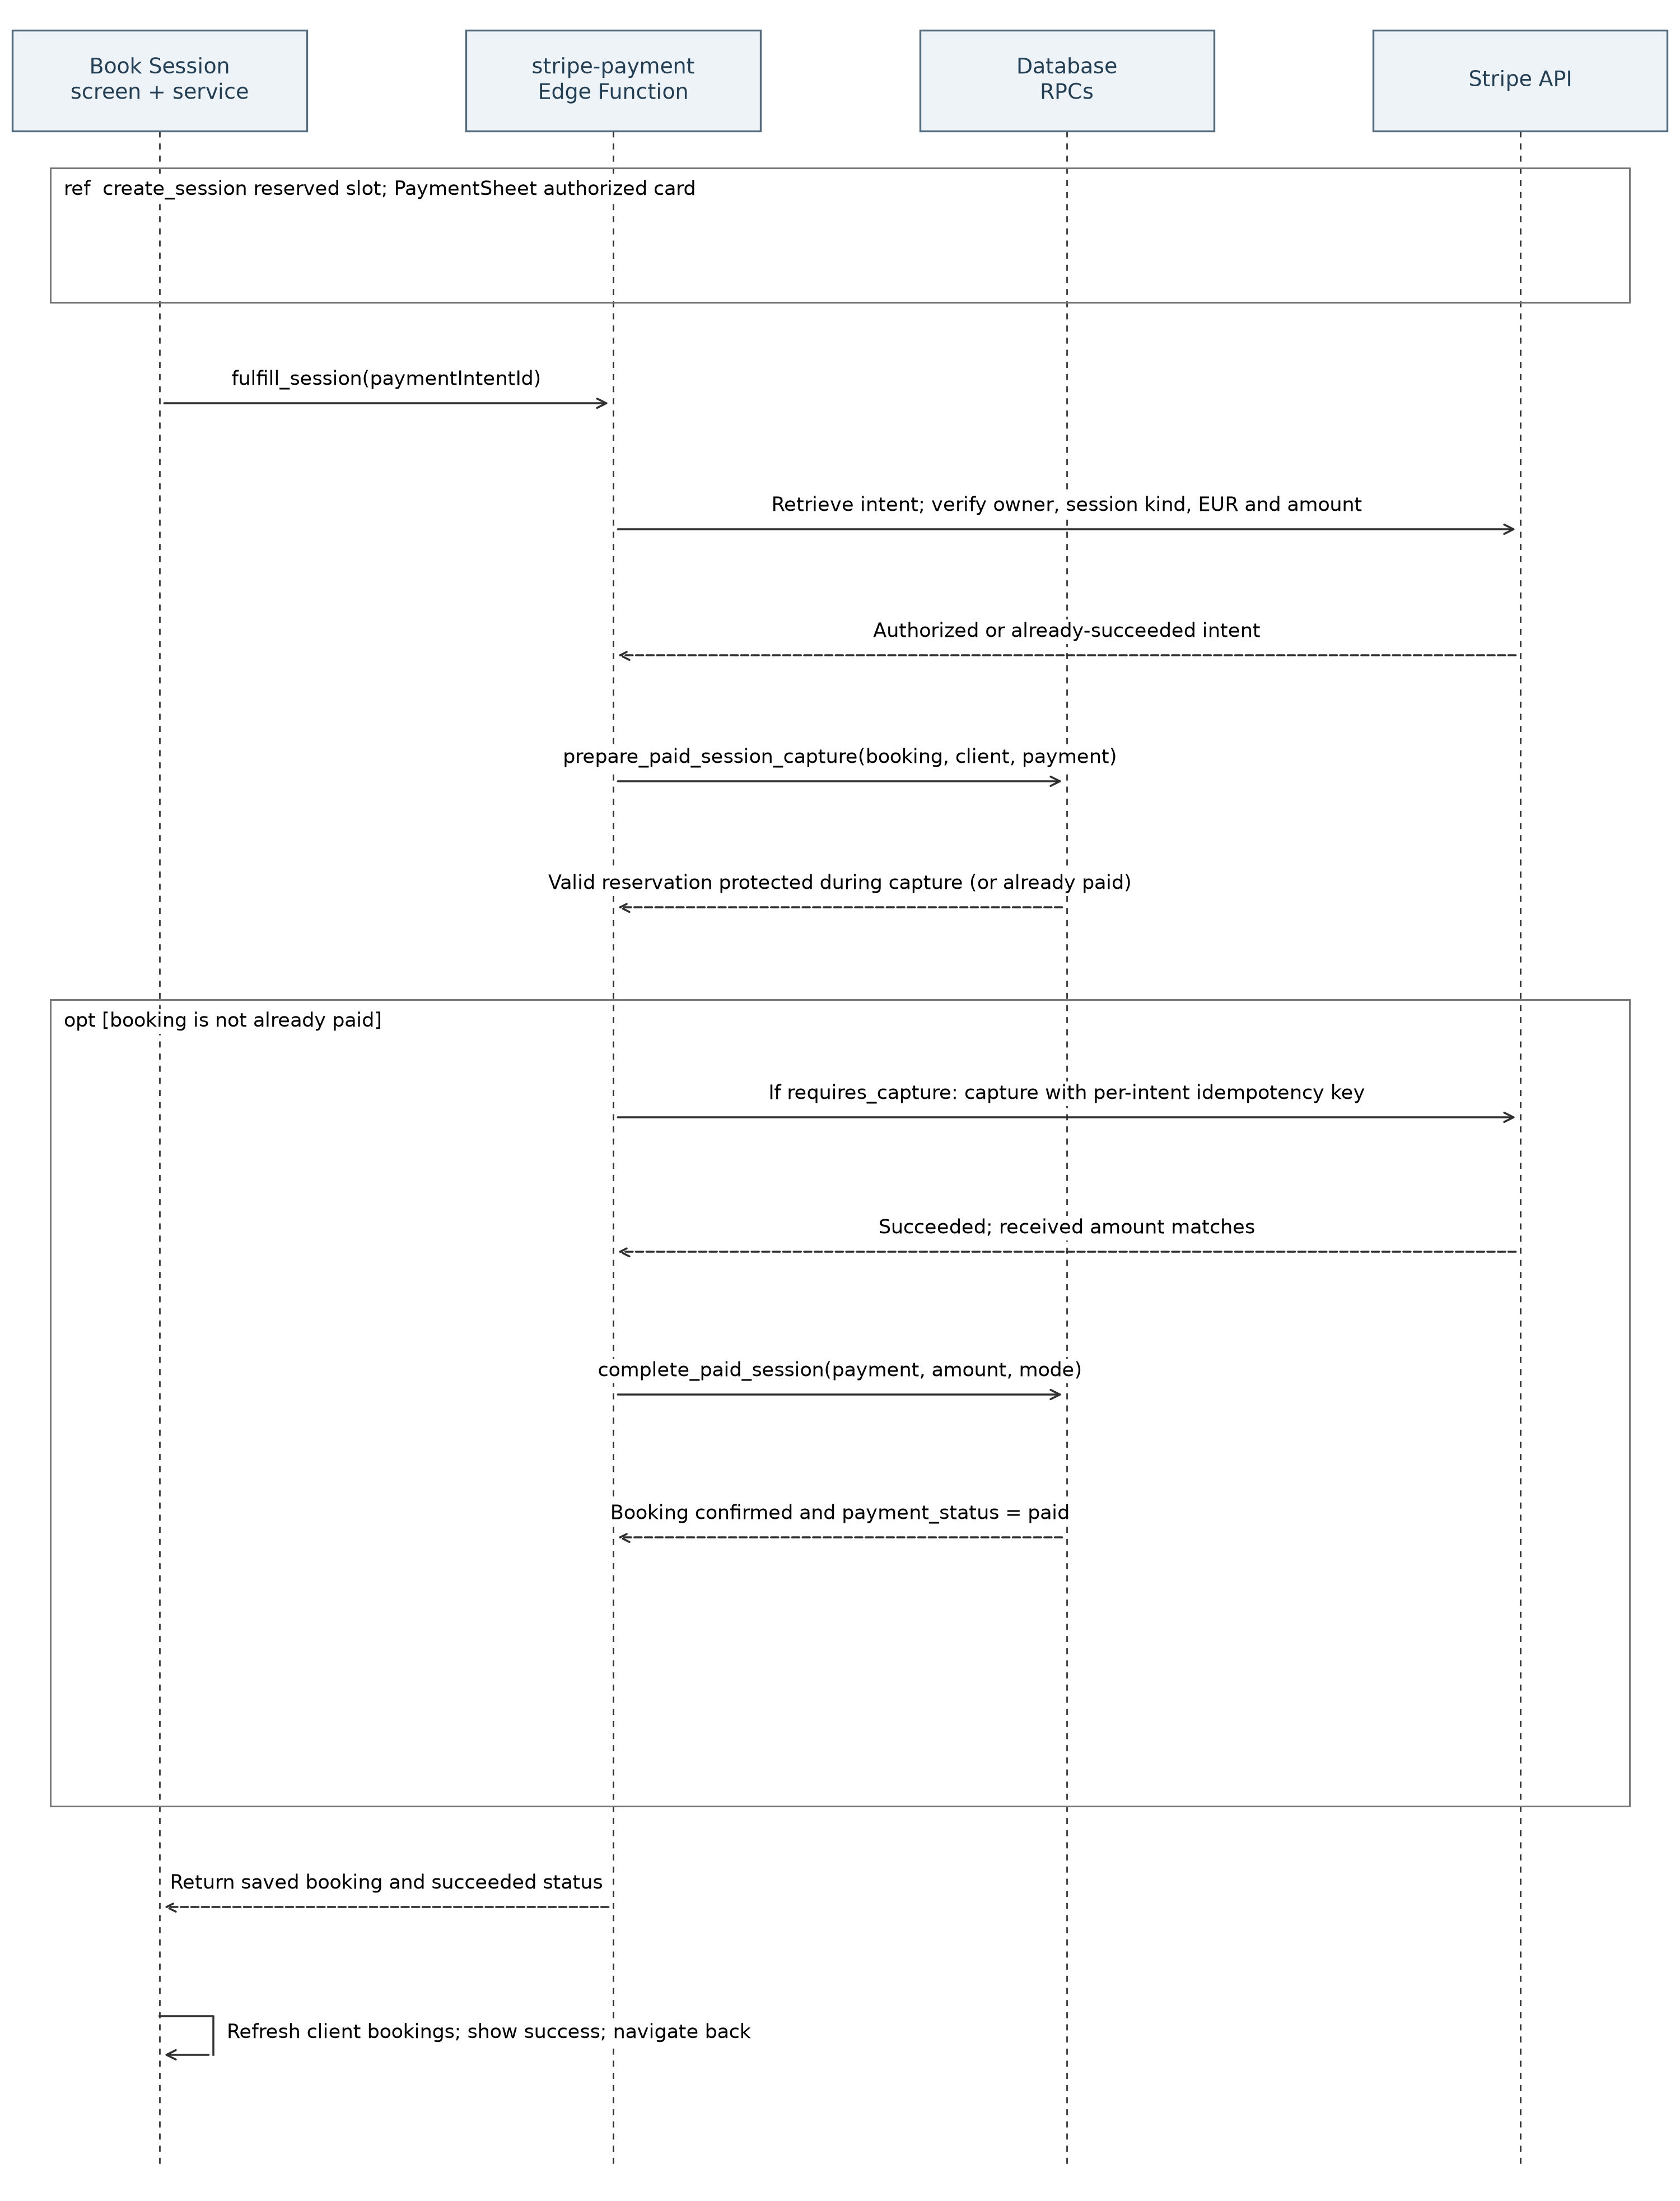
\includegraphics[width=0.95\linewidth]{figures/seq_booking_direct.png}
\caption{Technical sequence diagram: Reserved standalone session, capture and confirmation}
\label{fig:seq_booking_direct}
\end{figure}

Figure~\ref{fig:seq_booking_direct} follows standalone fulfilment after card authorization. The server verifies the owner and provider metadata, then calls \texttt{prepare\_paid\_session\_capture} to validate the reservation and protect it during capture. It captures an authorized intent using an idempotency key, checks the received amount, and calls \texttt{complete\_paid\_session} to mark the booking confirmed and paid. Already-paid replay returns the existing booking. The mobile screen refreshes client bookings before showing success. This corrected branch does not call the older client-side booking insertion and notification orchestration. Notification delivery is therefore not a postcondition established by this sequence. October API/provider and administrator readback evidence supports payment persistence; native standalone checkout remains pending.

The separate \texttt{createBooking} service still supports a purchased-pack reference and calls \texttt{deduct\_session} after insertion. Those requests are not one atomic booking-and-credit operation, and the standalone screen does not use that branch. Wallet transactions remain a different ledger from card purchase and booking payment snapshots. The selected cumulative class diagrams omit most financial attributes for readability: provider references, paid amount/currency/mode and booking payment state are attributes of the existing purchase and booking records, not a new persisted PaymentIntent entity. The diagrams do not establish coach payout settlement or automatic refund processing.

\subsubsection{Use case: Approve a coach profile from the administration panel}

\begingroup
\footnotesize
\setlength{\tabcolsep}{3pt}
\renewcommand{\arraystretch}{1.20}
\setlength{\LTpre}{5pt}
\setlength{\LTpost}{10pt}
\begin{longtable}{|L{4.95cm}|L{10.05cm}|}
\caption{Textual description of use case: Approve a coach profile from the administration panel}\label{tab:pdf-73-33} \\
\hline
\rowcolor{entetetab}
Field & Description \\ \hline
\endfirsthead
\hline
\rowcolor{entetetab}
Field & Description \\ \hline
\endhead
Use case & Approve a coach profile from the administration panel \\ \hline
Primary actor & Administrator \\ \hline
Preconditions & The administrator is authenticated and the account's \texttt{user\_profiles.is\_admin} flag permits administrative access. The selected approval path concerns a pending coach profile and requires working backend configuration. \\ \hline
Postconditions & On success, the profile has \texttt{status = approved} and \texttt{is\_verified = true}; the browser displays success and refreshes the table. The deployed approval-transition trigger creates a EUR wallet if none exists for that coach. This route does not explicitly insert an audit entry or send a coach notification. \\ \hline
Nominal scenario & 1. The administrator opens Coach Management at /coaches. 2. The table initially displays all statuses; the administrator selects Pending. 3. The administrator reviews the displayed profile information and may open the existing CV link when available. 4. The administrator selects Approve and confirms the dialog. 5. The browser sends a PATCH request to /api/coaches. 6. The server checks administrative access, validates the input, and updates the coach profile. 7. The database approval trigger ensures a wallet exists; the route returns the updated profile, and the browser displays success and refreshes the list. \\ \hline
Alternative scenario & 4.1. Rejection submits \texttt{status = rejected} without a feedback field or required reason. Approved coaches can be revoked and rejected coaches re-approved through separate confirmation dialogs. Certification-record verification uses a separate API endpoint and is not performed by this profile-approval action. \\ \hline
Exception scenario & E.1. Protected page access without a suitable session redirects to Login; unauthenticated API access returns 401 and authenticated non-admin API access returns 403 at the proxy. The route also verifies administrative access. E.2. Missing or invalid input returns 400; a profile-update failure returns an error response. E.3. A failed PATCH response produces an error toast. With no CV URL, the table provides no View CV action; document availability is not validated by the approval handler. \\ \hline
\end{longtable}
\endgroup

\begin{figure}[H]
\centering
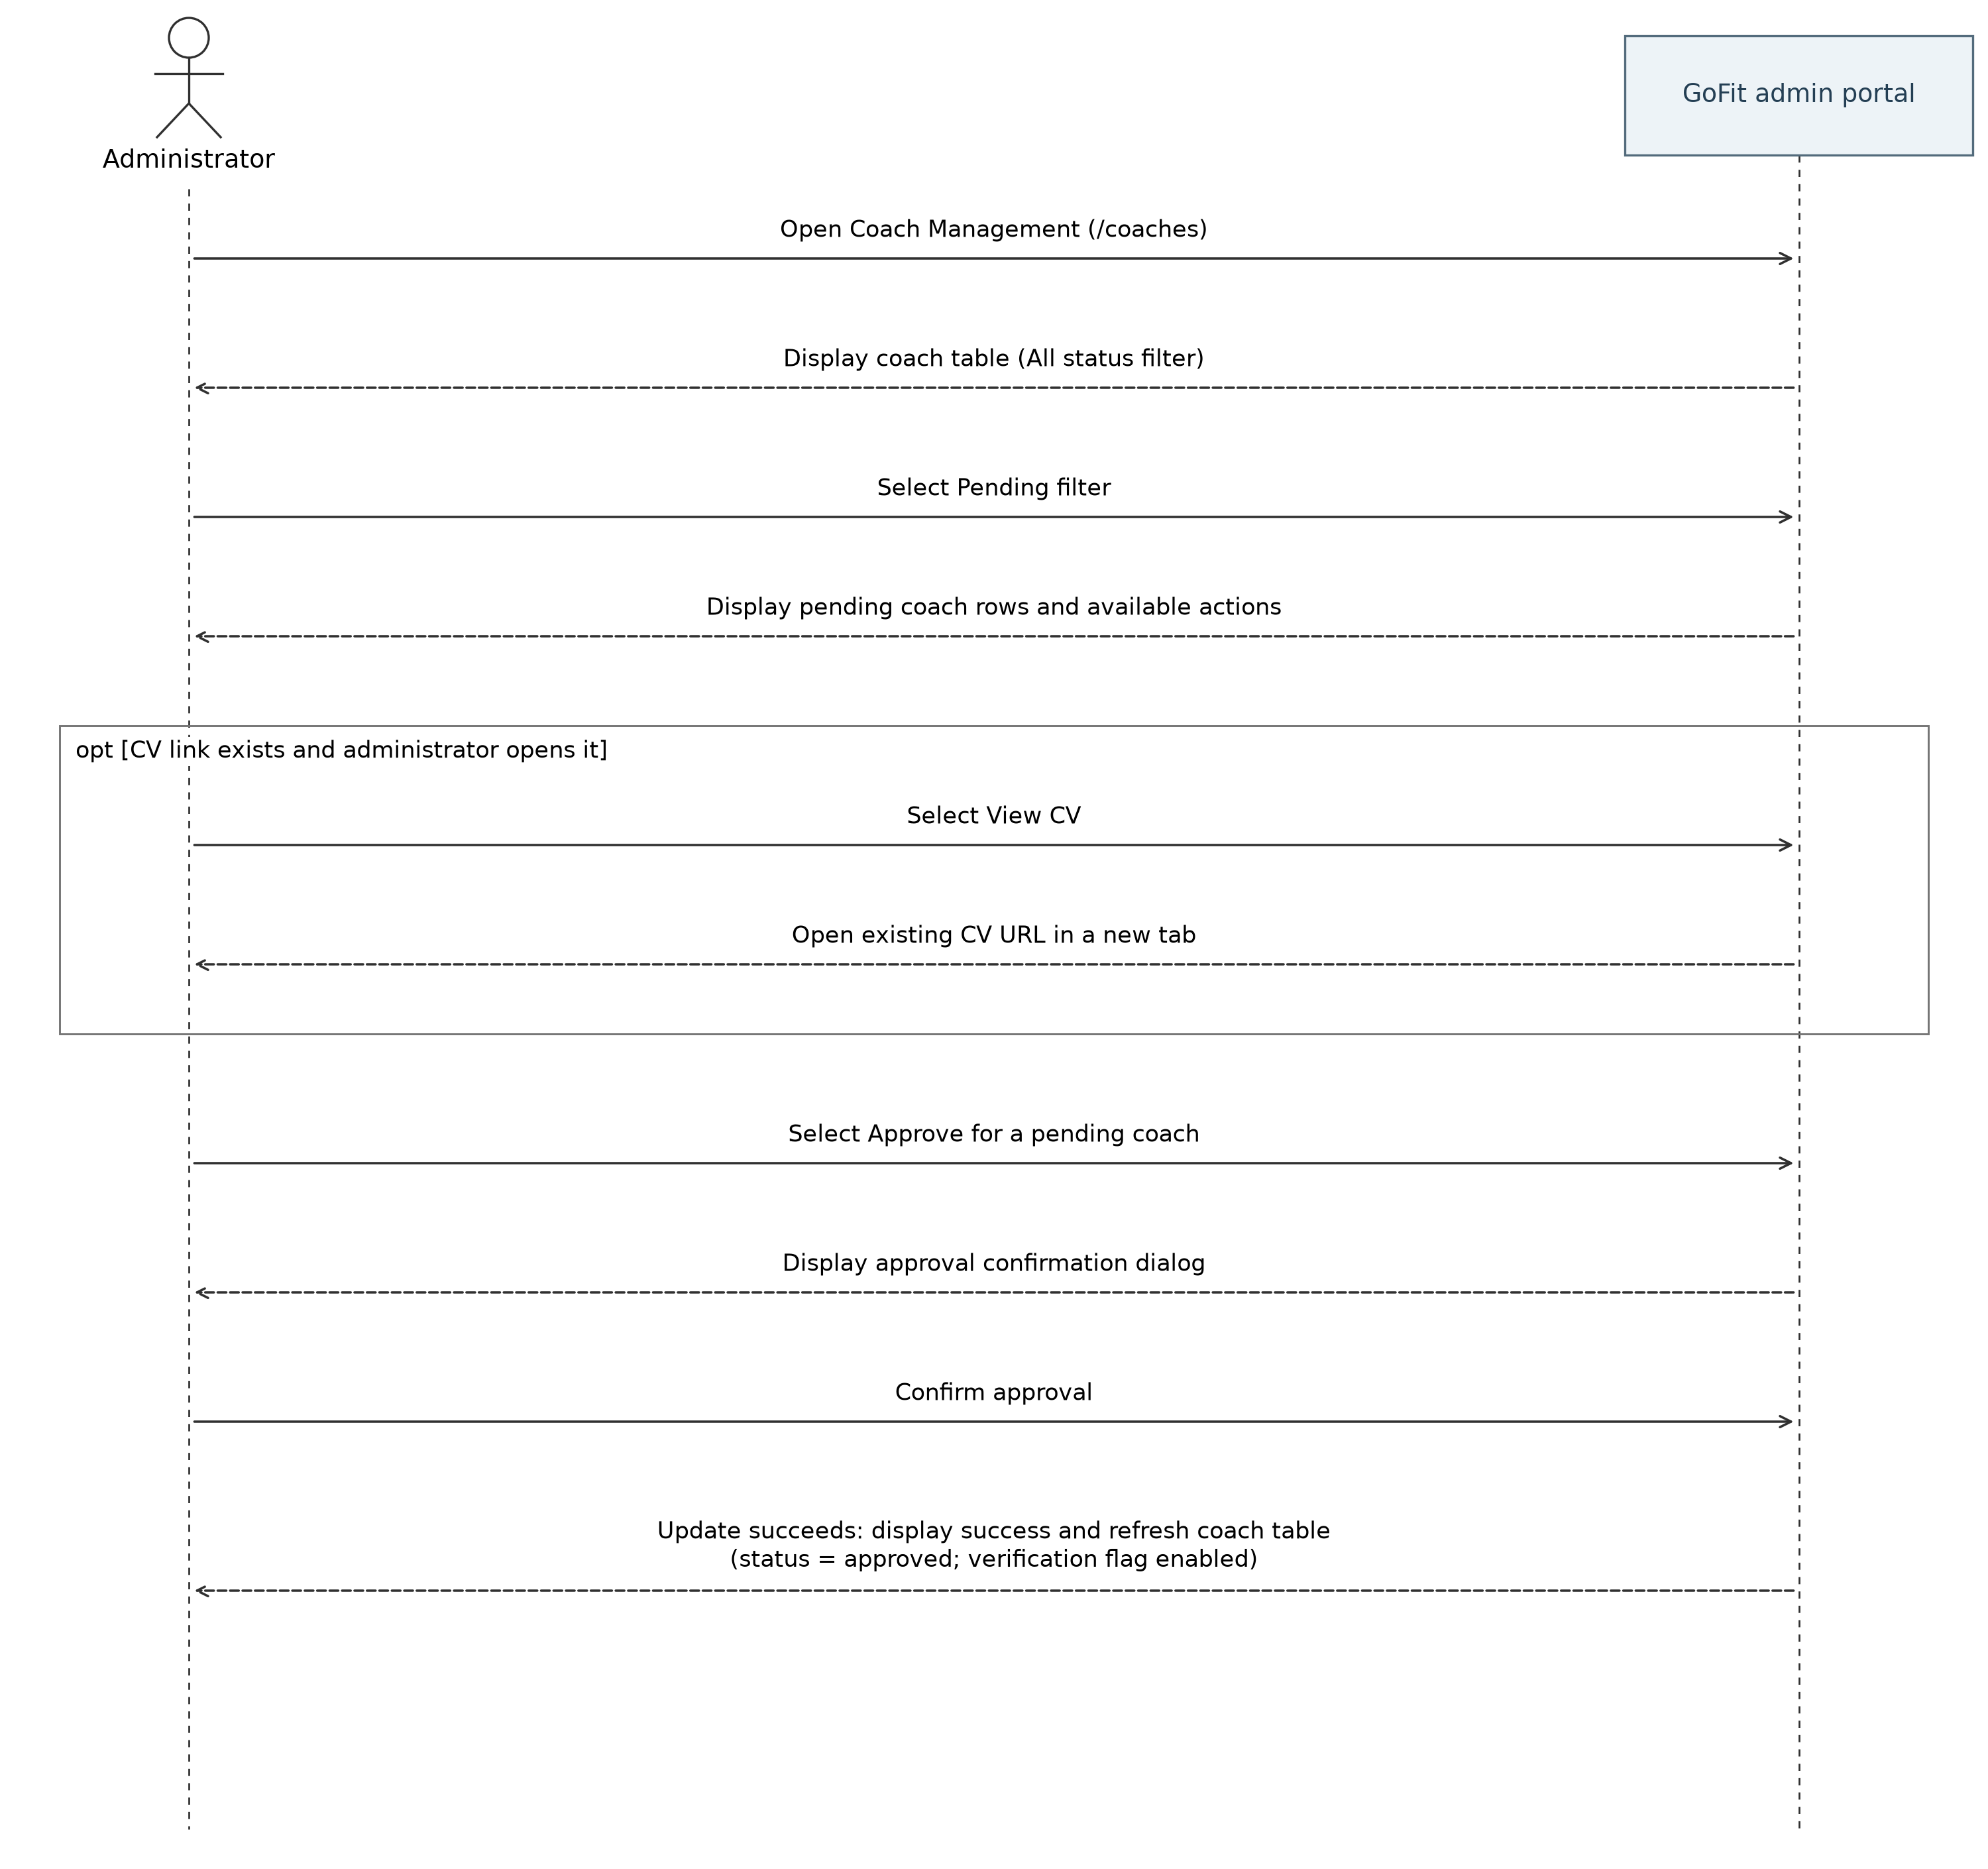
\includegraphics[width=0.92\linewidth]{figures/seq_admin_audit_ssd.png}
\caption{System sequence diagram: Administrator review and successful coach-profile approval}
\label{fig:seq_admin_audit_ssd}
\end{figure}

\begin{figure}[H]
\centering
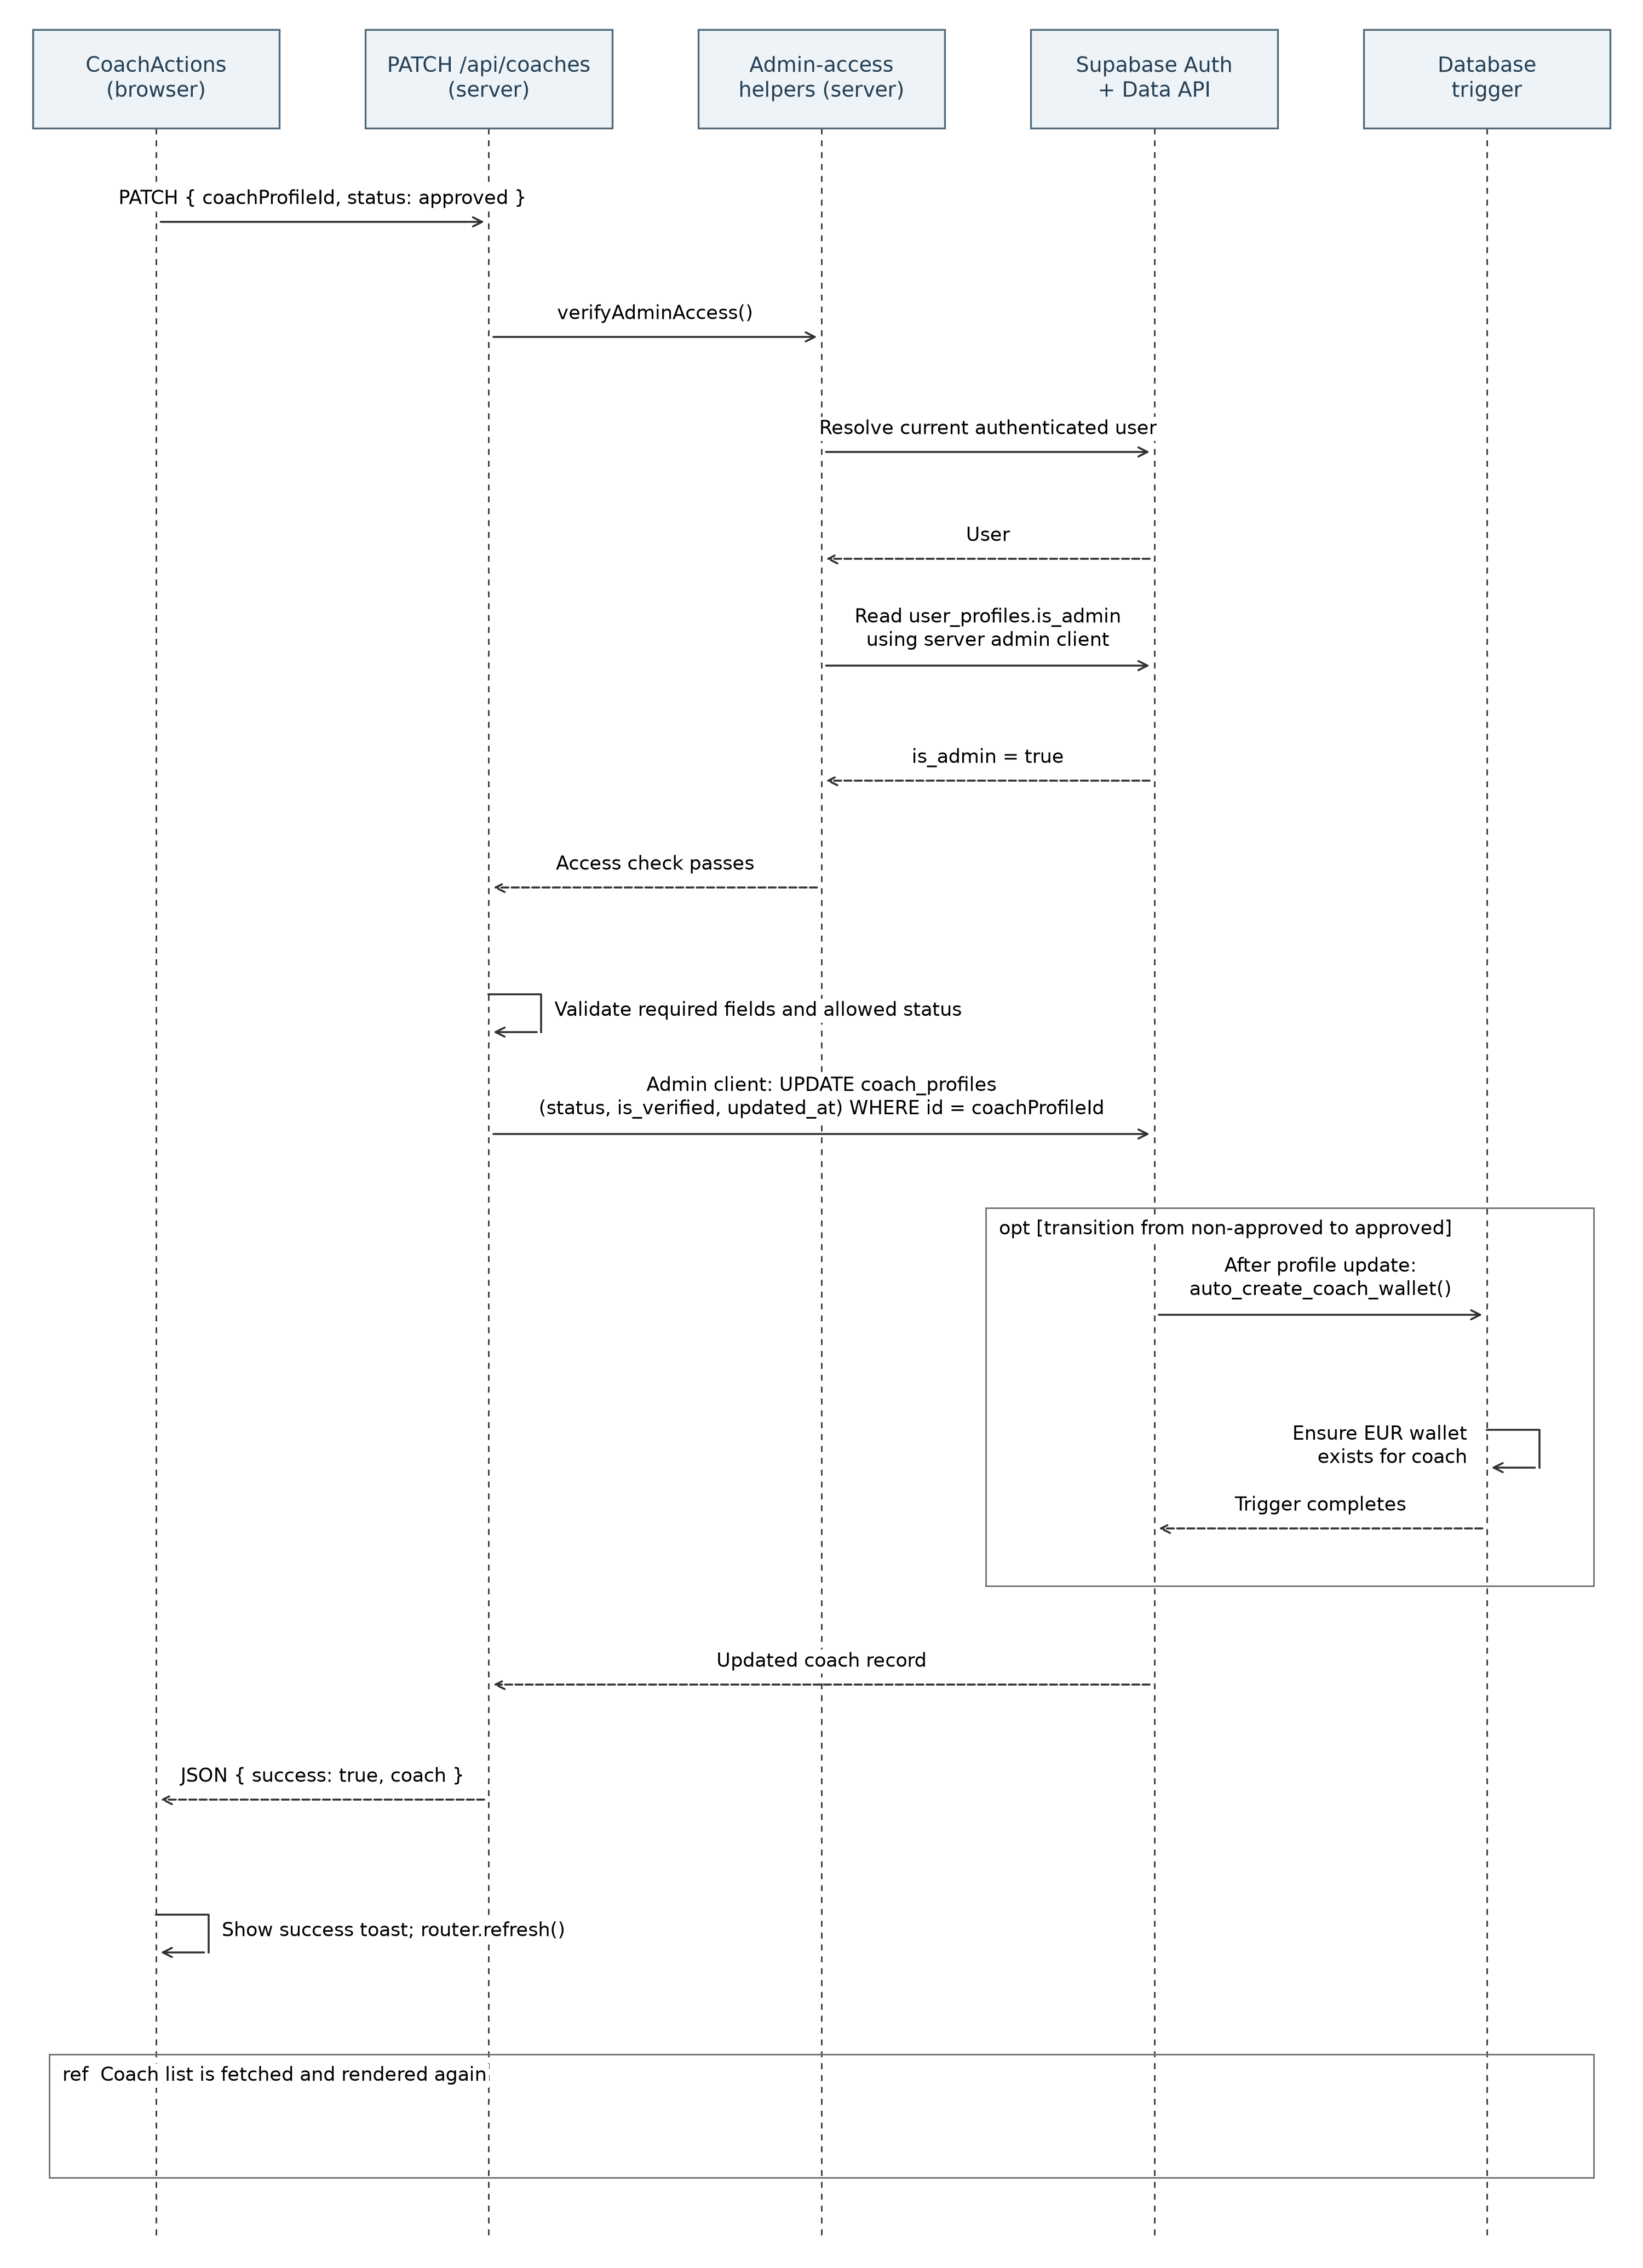
\includegraphics[width=0.92\linewidth]{figures/seq_admin_audit_detailed.png}
\caption{Technical sequence diagram: Protected coach-profile update and deployed wallet trigger}
\label{fig:seq_admin_audit_detailed}
\end{figure}

Figure~\ref{fig:seq_admin_audit_ssd} follows the visible Coach Management workflow. The list starts with an All status filter; Pending is an administrator selection. The table displays profile information and provides a View CV link when the stored \texttt{cv\_url} is present. That link opens the existing URL in a new tab. The inspected page and action component do not generate signed document URLs, present a separate certification-review screen, or require evidence of document inspection before approval. The sequence therefore represents administrative profile approval rather than proof that professional accreditation has been independently validated.

Figure~\ref{fig:seq_admin_audit_detailed} begins with the confirmed approval request from CoachActions. Its PATCH request contains \texttt{coachProfileId} and \texttt{status}; it is handled by an API route rather than a server action. The route calls \texttt{verifyAdminAccess()}, which resolves the current user through the cookie-aware server client and reads \texttt{user\_profiles.is\_admin} using a server-side admin client. It then validates required fields and the allowed statuses: approved, rejected, and pending. For approval, the admin client updates \texttt{coach\_profiles.status}, sets \texttt{is\_verified} to true, supplies an updated timestamp, and retrieves the affected profile. Administrative credentials remain in the server-side client boundary shown by the diagram. The technical sequence selects the authorized successful path; the request proxy's earlier checks are described in the use-case table rather than repeated as diagram participants.

Read-only inspection of the deployed \texttt{coach\_profiles} triggers confirmed timestamp maintenance and \texttt{trigger\_auto\_create\_coach\_wallet}. When status changes from non-approved to approved, the latter inserts a EUR wallet with conflict handling that leaves an existing coach wallet in place. The database-trigger participant summarizes this internal database operation, not a separate external service. After the update succeeds, the route returns a JSON success response with the coach record; CoachActions displays a toast and calls \texttt{router.refresh()} to fetch and render the list again. The diagram does not establish a successful browser approval test merely from the presence of these implementations.

Coach-profile approval is distinct from certification-record verification. A separate endpoint, \texttt{/api/coaches/[id]/certifications}, updates a selected \texttt{coach\_certifications} record using statuses verified, rejected, or pending and sets its verification timestamp when appropriate. The profile-approval route does not invoke that endpoint. Although the project contains a general audit utility, this route does not call it, and the inspected coach-profile triggers do not add an audit entry or send a welcome email or coach notification. An immutable approval-audit trail and automatic coach messaging are therefore not claimed for this workflow. The current rejection action also has no reason field; its status update sets the profile verification flag to false.


\section{Realisation}

The coach marketplace enables discovery of certified coaches with specialties, hourly rates, client ratings, and multi-session package offerings.


The dedicated coach workspace includes a client roster, check-in review timeline, custom workout and nutrition assignment tools, and private coaching notes.


Communication combines chat subscriptions through Supabase Realtime with LiveKit WebRTC integration for 1-on-1 video calls. The source establishes these integration paths; it does not establish a measured latency bound or successful calls across all target devices.


The Next.js administration portal applies server-side role checks to coach-profile approval, exercise catalog management, financial-record inspection, and platform BI analytics. Viewing activity logs does not imply that every administrative operation creates a log entry; the inspected coach-approval path does not write an audit record or dispatch an approval notification.


\subsection{Coach Marketplace and Client Follow-up}

Sprint 3 expanded GoFit from an individual fitness tracker into a marketplace and coaching platform. This required a different type of workflow because the application now connects two human roles: the client and the coach. The client needs to discover coaches, view profiles, book sessions, purchase packs, access programs, and communicate. The coach needs to onboard, submit profile and document information, wait for validation when required, manage availability, consult clients, create programs, read notes, and follow progress.


The marketplace is not only a list of coaches. It depends on trust, availability, transaction status, communication, and follow-up. For this reason, the sprint includes coach profiles, session packs, bookings, purchased packs, conversations, messages, programs, notifications, and wallet-related views. Each of these elements must be connected to permissions so that clients can see their own bookings and coaches can see only their own clients.


\begingroup
\footnotesize
\setlength{\tabcolsep}{3pt}
\renewcommand{\arraystretch}{1.20}
\setlength{\LTpre}{5pt}
\setlength{\LTpost}{10pt}
\begin{longtable}{|L{3.67cm}|L{5.29cm}|L{5.73cm}|}
\caption{Coach marketplace feature detail}\label{tab:pdf-76-34} \\
\hline
\rowcolor{entetetab}
Feature & Client-side value & Coach-side value \\ \hline
\endfirsthead
\hline
\rowcolor{entetetab}
Feature & Client-side value & Coach-side value \\ \hline
\endhead
Coach discovery & Find coaches by profile, expertise, and services. & Increase visibility and attract clients. \\ \hline
Coach onboarding & Improves trust by requiring complete coach data. & Allows coach to create a professional presence. \\ \hline
Session packs & Buy or use grouped coaching sessions. & Sell structured services and track remaining sessions. \\ \hline
Bookings & Reserve a coaching slot and follow status. & Organize calendar and session workload. \\ \hline
Programs & Receive personalized training plans. & Create and assign plans to clients. \\ \hline
Chat and notes & Communicate with the coach and receive follow-up. & Keep client context and preparation notes together. \\ \hline
Video call screen & Join remote coaching sessions. & Connect with clients through LiveKit-backed sessions. \\ \hline
\end{longtable}
\endgroup

Figures~\ref{fig:ui-coaching-availability} and~\ref{fig:ui-coach-workspace} show selected coaching interfaces. The duration image records the restored 60-minute preference; it does not complete the pending native standalone-payment test. The program form is unsubmitted, the private note is a disposable QA fixture, and the conversation list is empty.

\begin{figure}[H]
\centering
\begin{minipage}[t]{.29\linewidth}
\centering

\includegraphics[width=\linewidth]{figures/screenshots/client-coach-discovery.png}
\par\smallskip{\footnotesize a) Client marketplace\par}
\end{minipage}
\hspace{0.025\linewidth}
\begin{minipage}[t]{.29\linewidth}
\centering
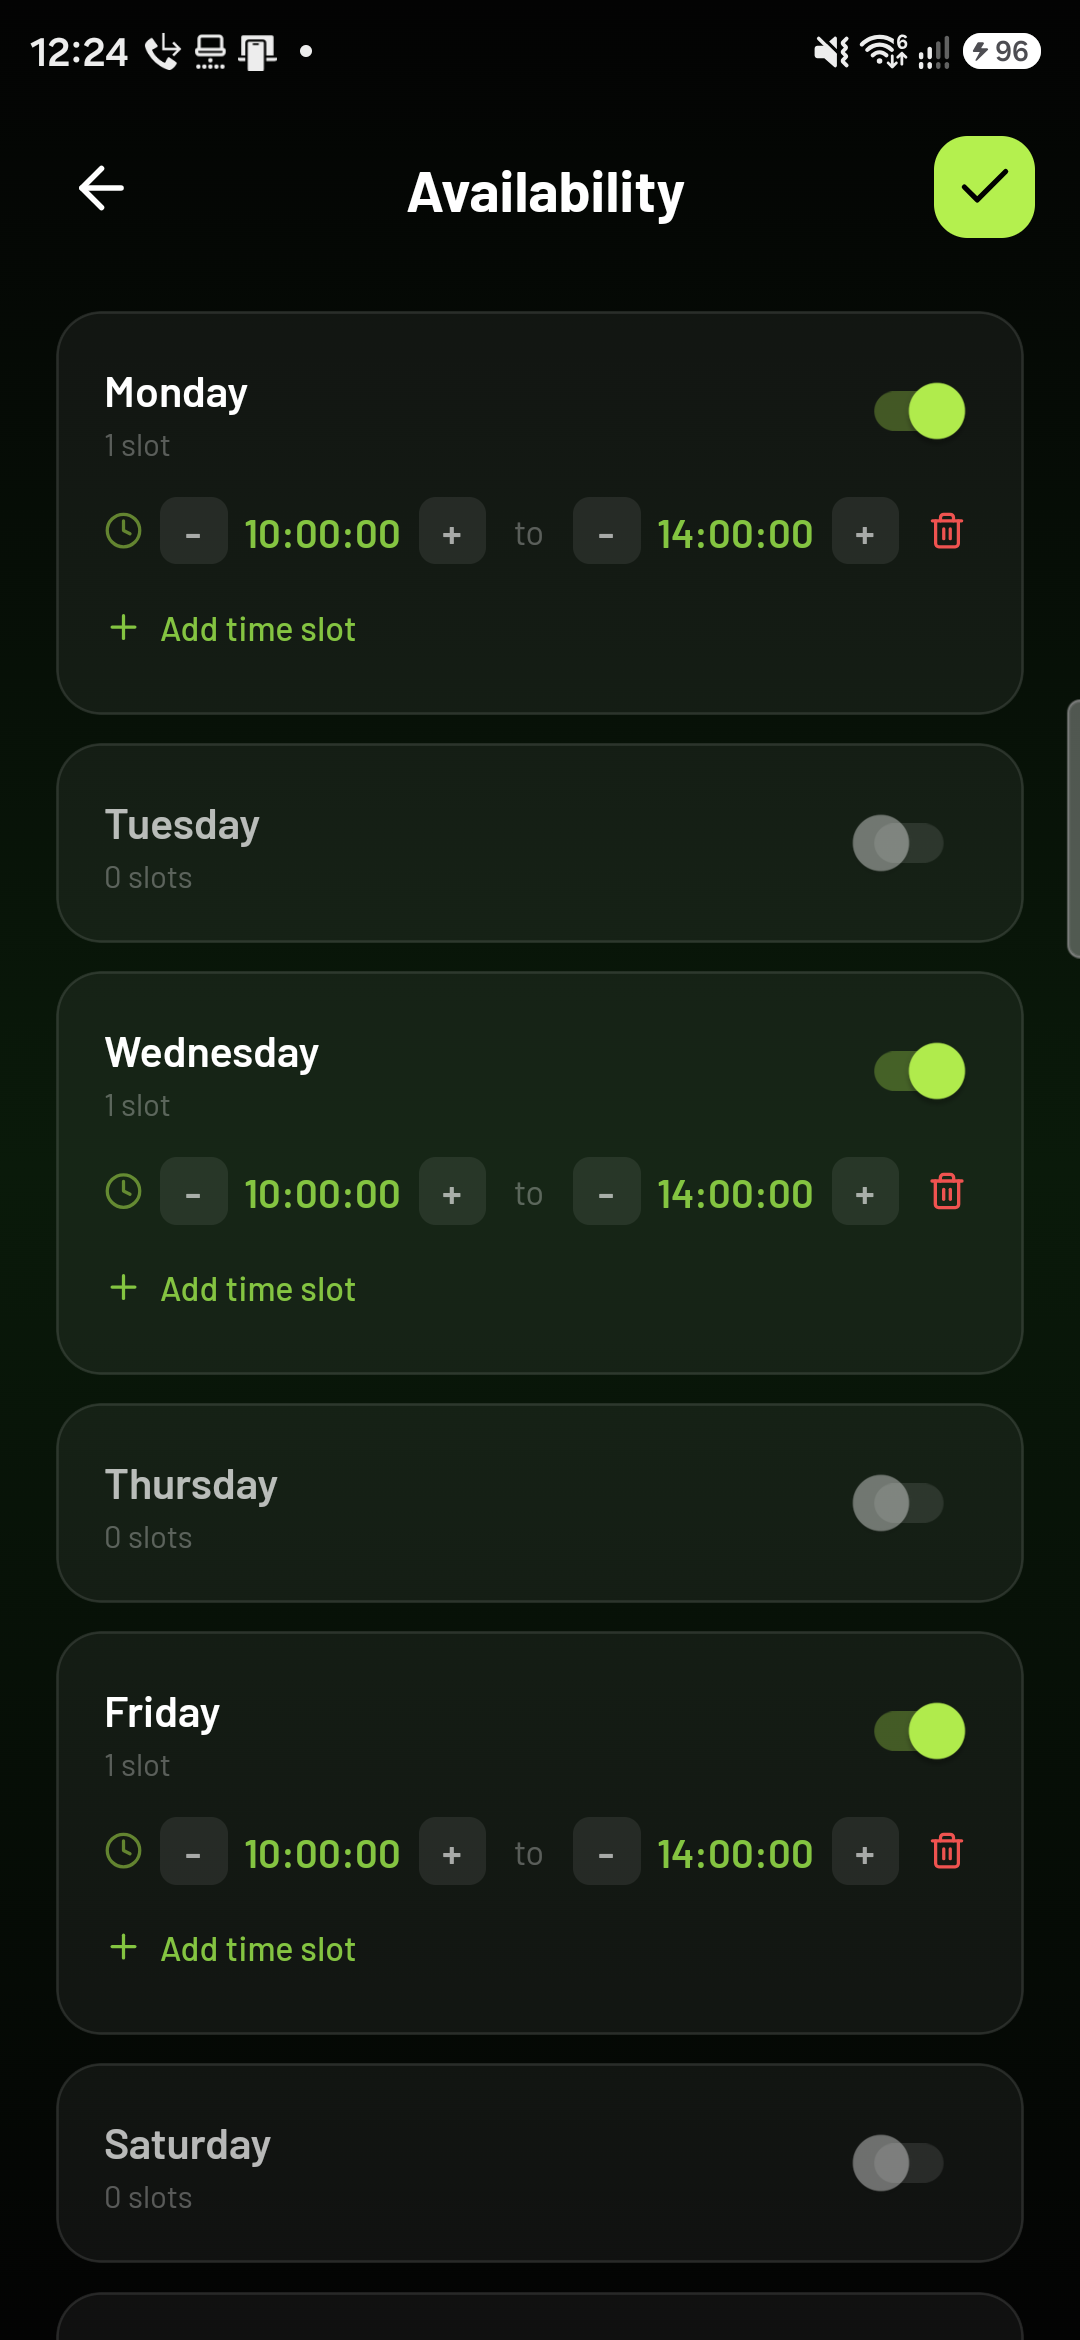
\includegraphics[width=\linewidth]{figures/screenshots/coach-availability.png}
\par\smallskip{\footnotesize b) Coach availability\par}
\end{minipage}
\hspace{0.025\linewidth}
\begin{minipage}[t]{.29\linewidth}
\centering
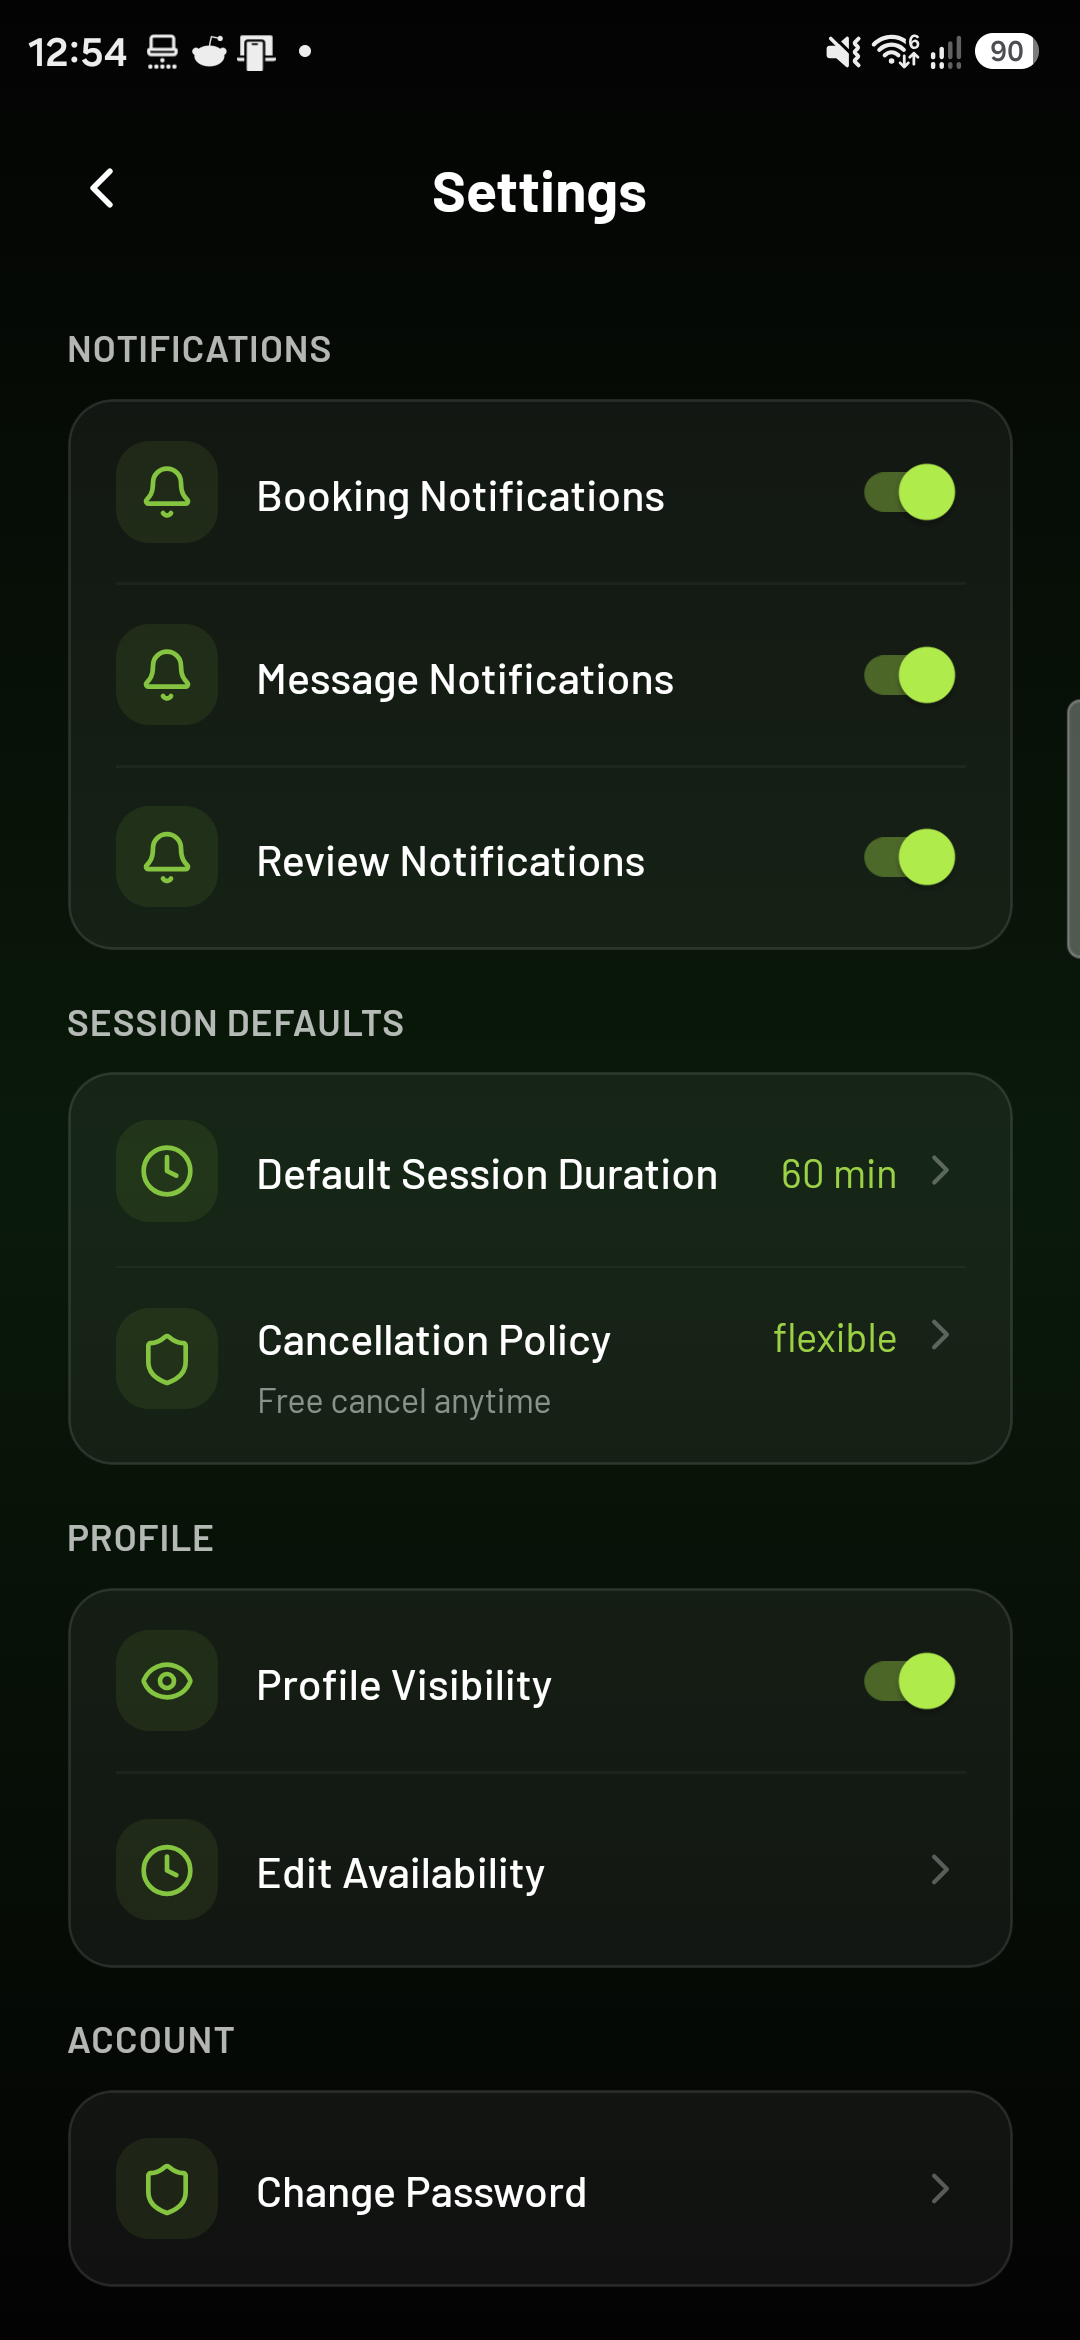
\includegraphics[width=\linewidth]{figures/screenshots/coach-saved-duration.png}
\par\smallskip{\footnotesize c) Saved duration restored to 60 min\par}
\end{minipage}
\caption{Interface captures: coach discovery, recurring availability and the restored session-duration preference.}
\label{fig:ui-coaching-availability}
\end{figure}

\begin{figure}[H]
\centering
\begin{minipage}[t]{.29\linewidth}
\centering
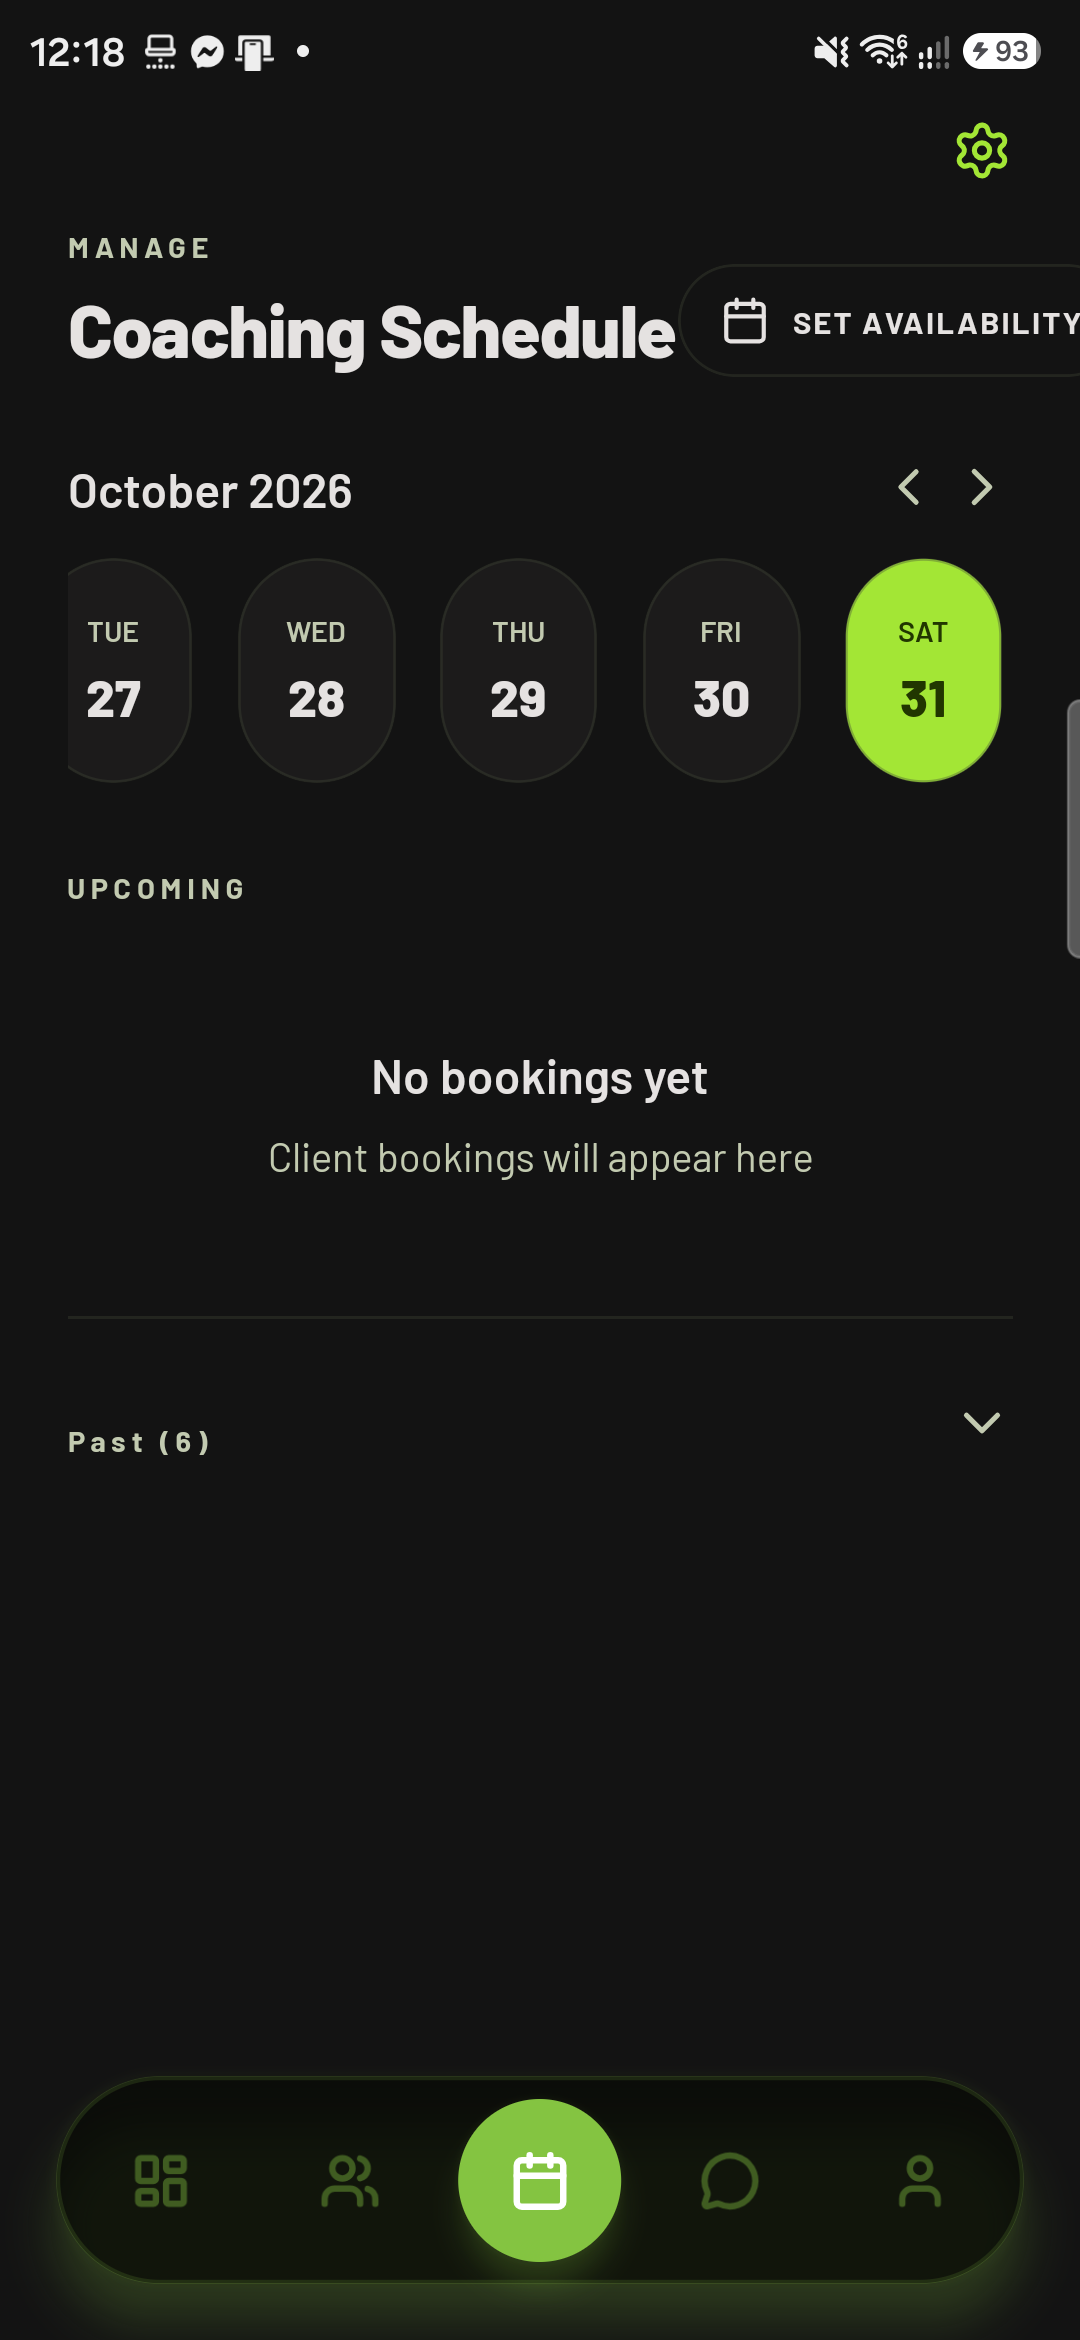
\includegraphics[width=\linewidth]{figures/screenshots/coach-calendar.png}
\par\smallskip{\footnotesize a) Calendar and empty upcoming list\par}
\end{minipage}
\hspace{0.025\linewidth}
\begin{minipage}[t]{.29\linewidth}
\centering
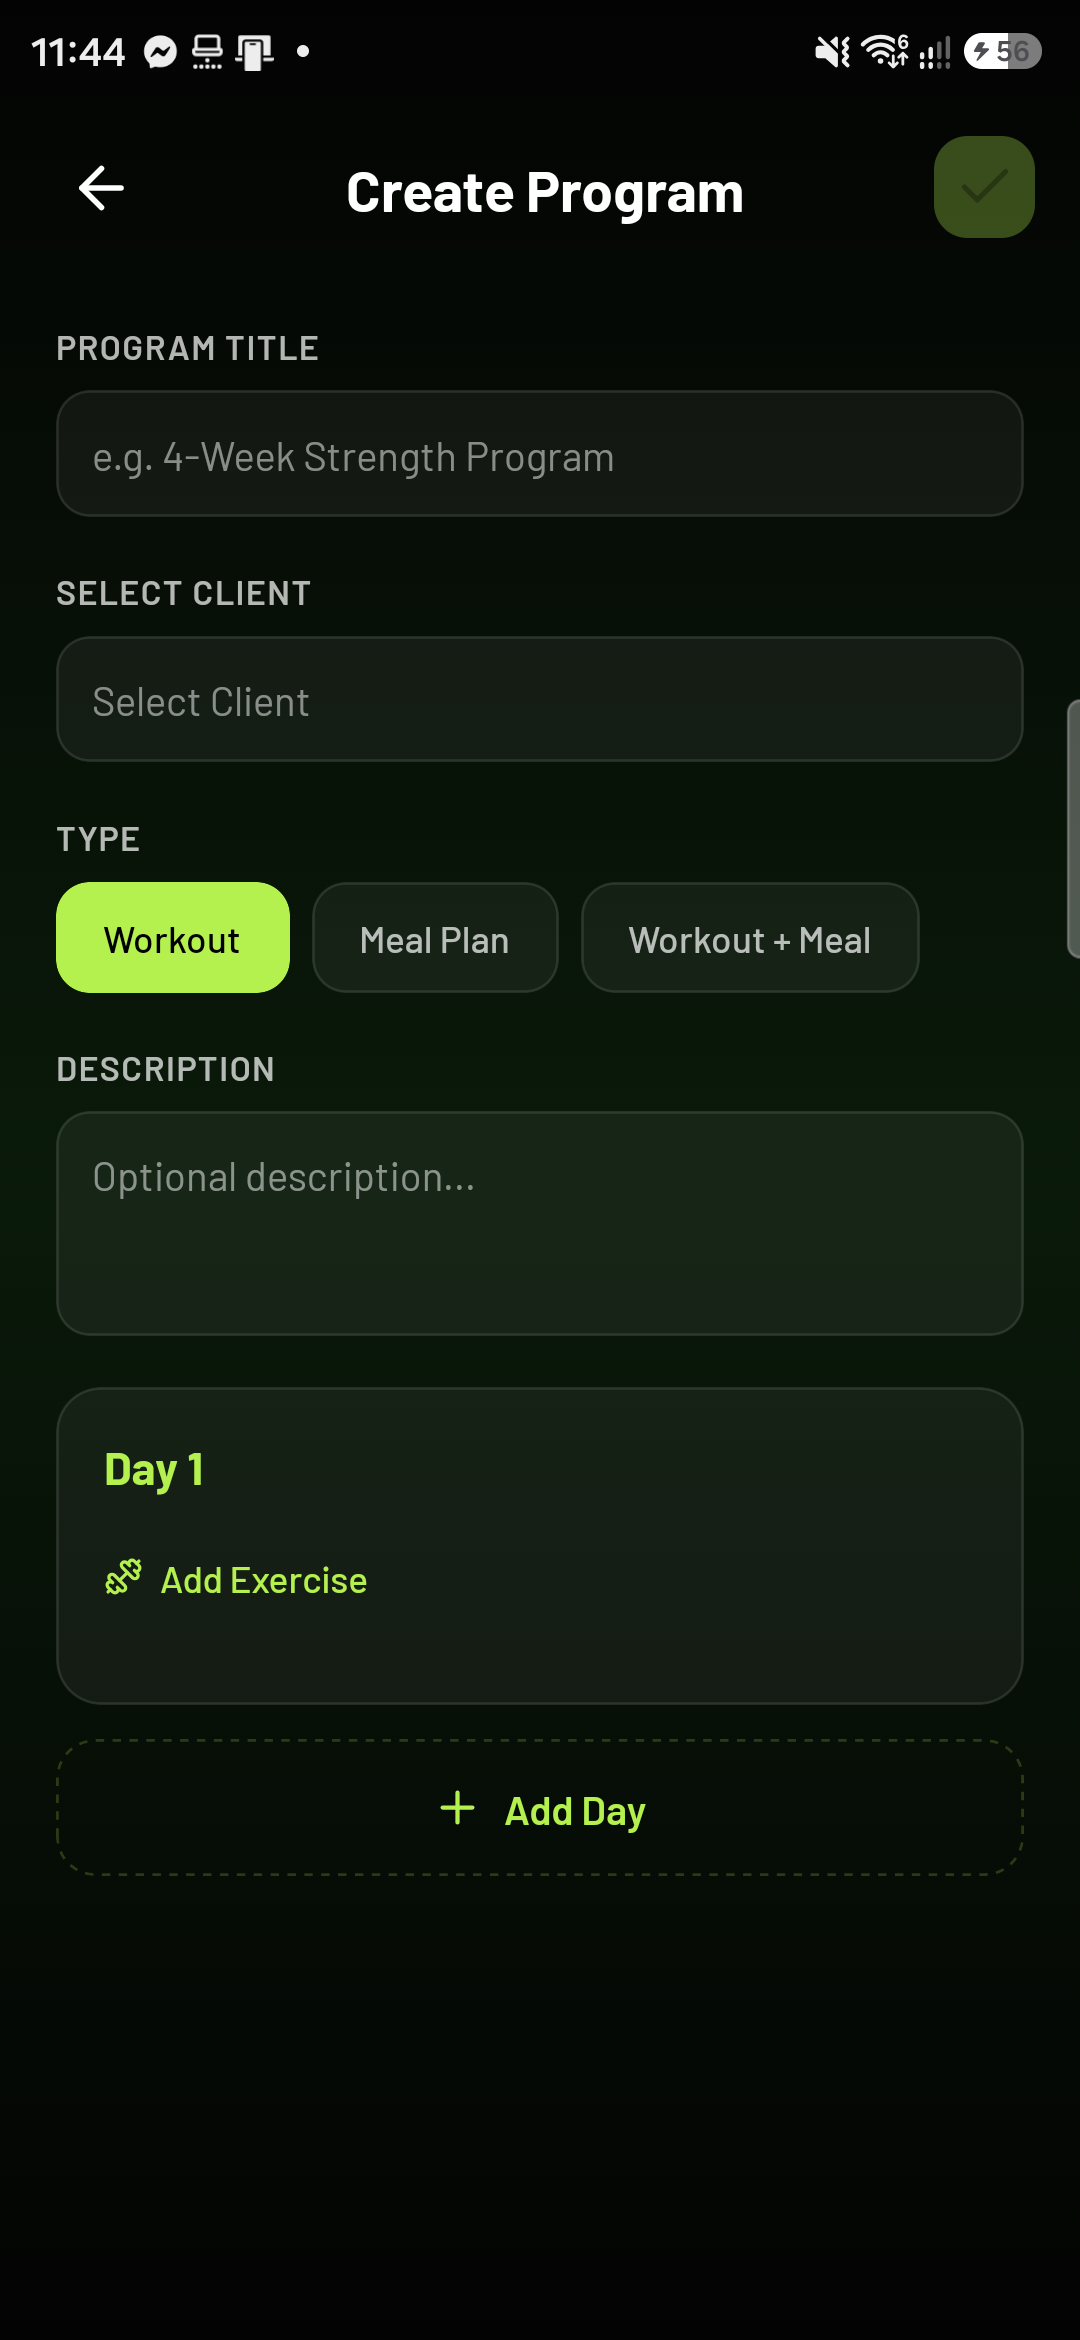
\includegraphics[width=\linewidth]{figures/screenshots/coach-program-form.png}
\par\smallskip{\footnotesize b) Program-creation form\par}
\end{minipage}
\hspace{0.025\linewidth}
\begin{minipage}[t]{.29\linewidth}
\centering

\includegraphics[width=\linewidth]{figures/screenshots/coach-disposable-note.png}
\par\smallskip{\footnotesize c) Disposable QA note\par}
\end{minipage}
\caption{Interface captures: coach calendar, unsubmitted program form and disposable private note.}
\label{fig:ui-coach-workspace}
\end{figure}

Figures~\ref{fig:ui-coach-followup-extended} and~\ref{fig:ui-coach-program-pack} expand the coaching views. Client identifiers are masked where present. The program remains an unsubmitted draft, the check-in schedule is displayed without a new submission, and the sample pack is an offer rather than proof of a payout.

\begin{figure}[H]
\centering
\begin{minipage}[t]{.29\linewidth}
\centering
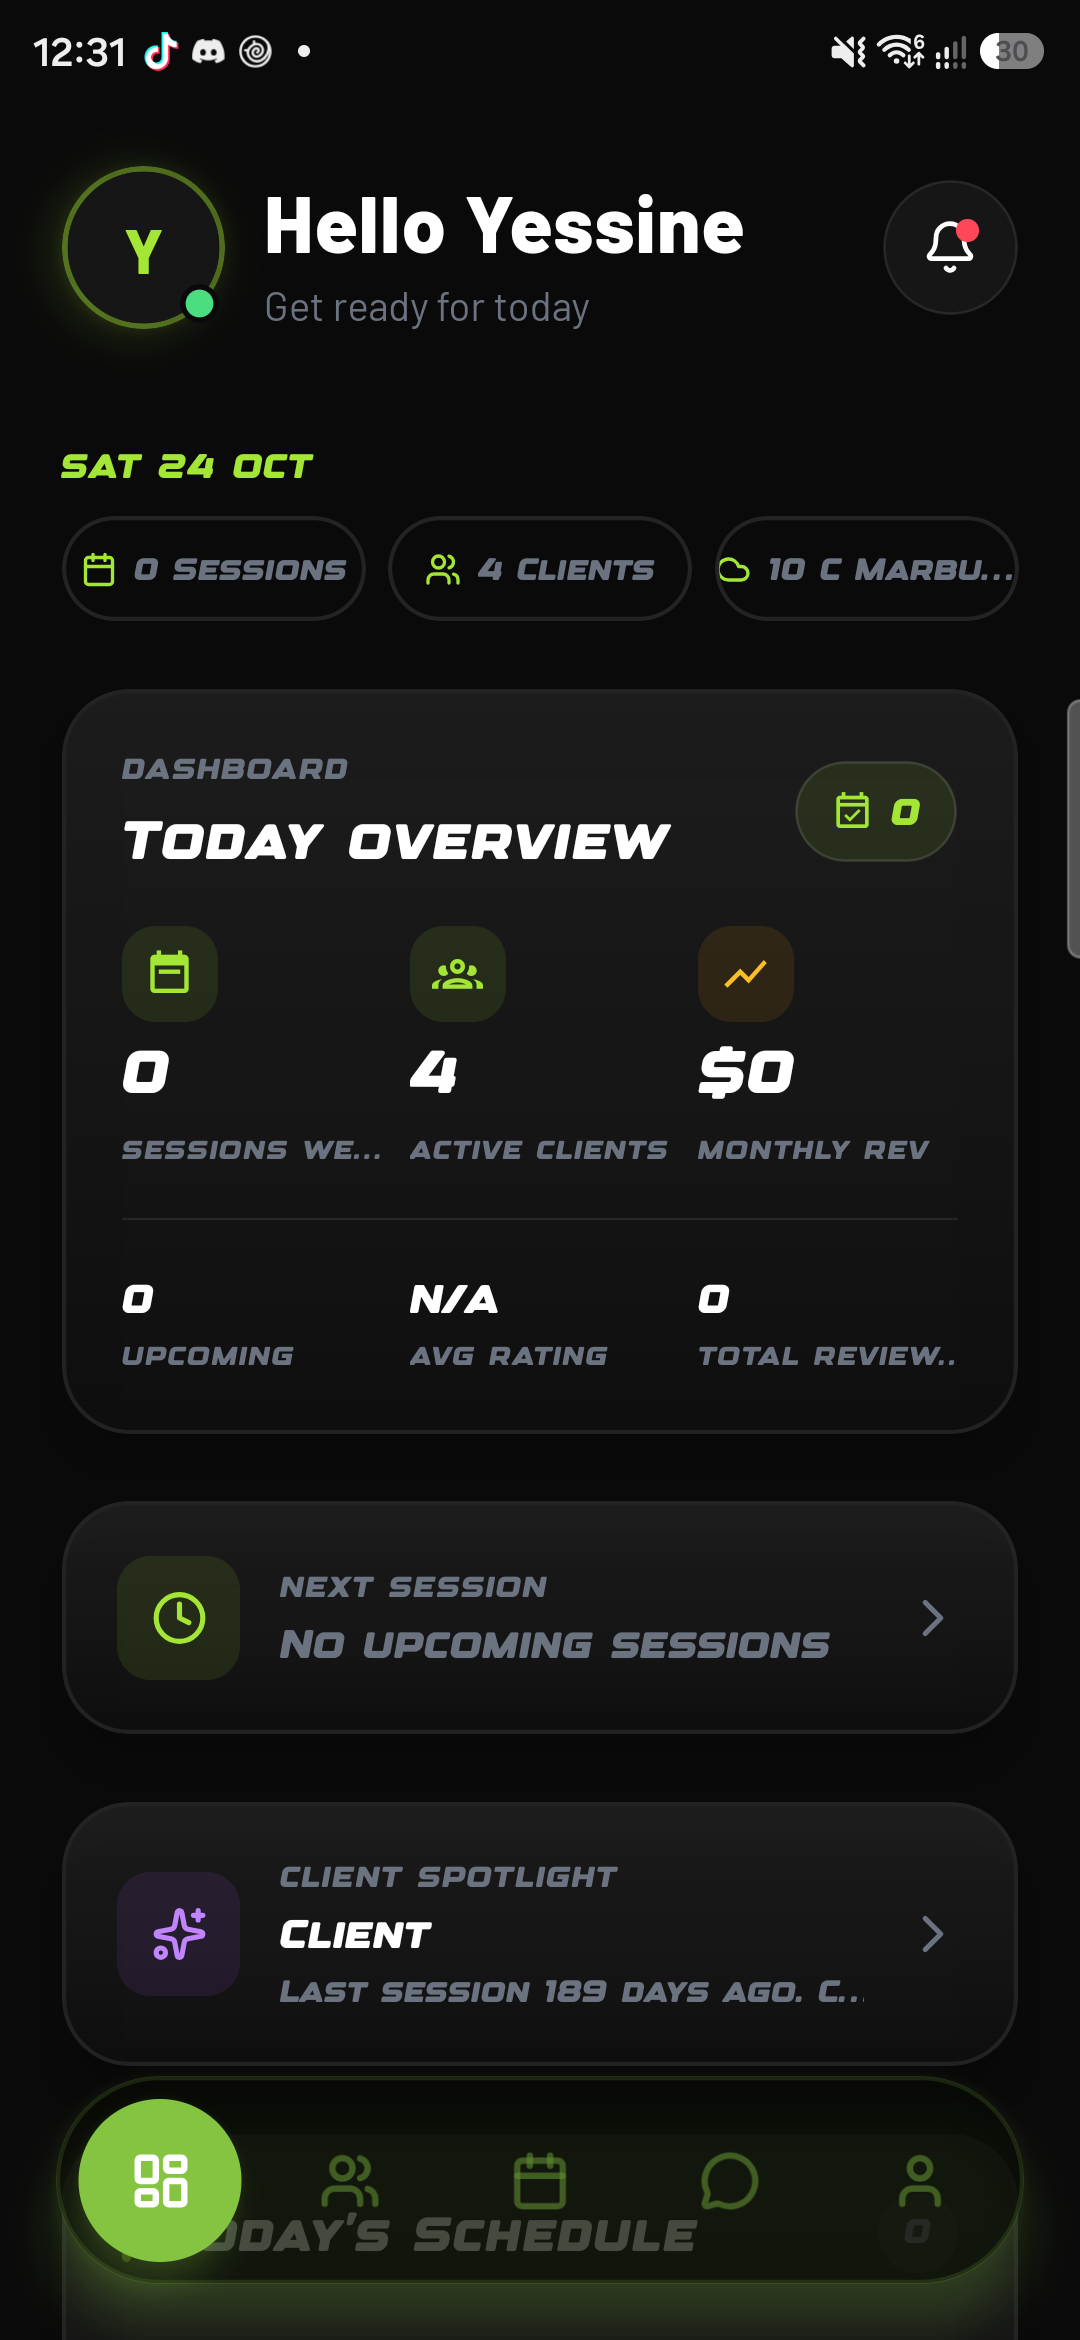
\includegraphics[width=\linewidth]{figures/screenshots/coach-dashboard-clean.png}
\par\smallskip{\footnotesize a) Dashboard after the query correction\par}
\end{minipage}
\hspace{0.025\linewidth}
\begin{minipage}[t]{.29\linewidth}
\centering
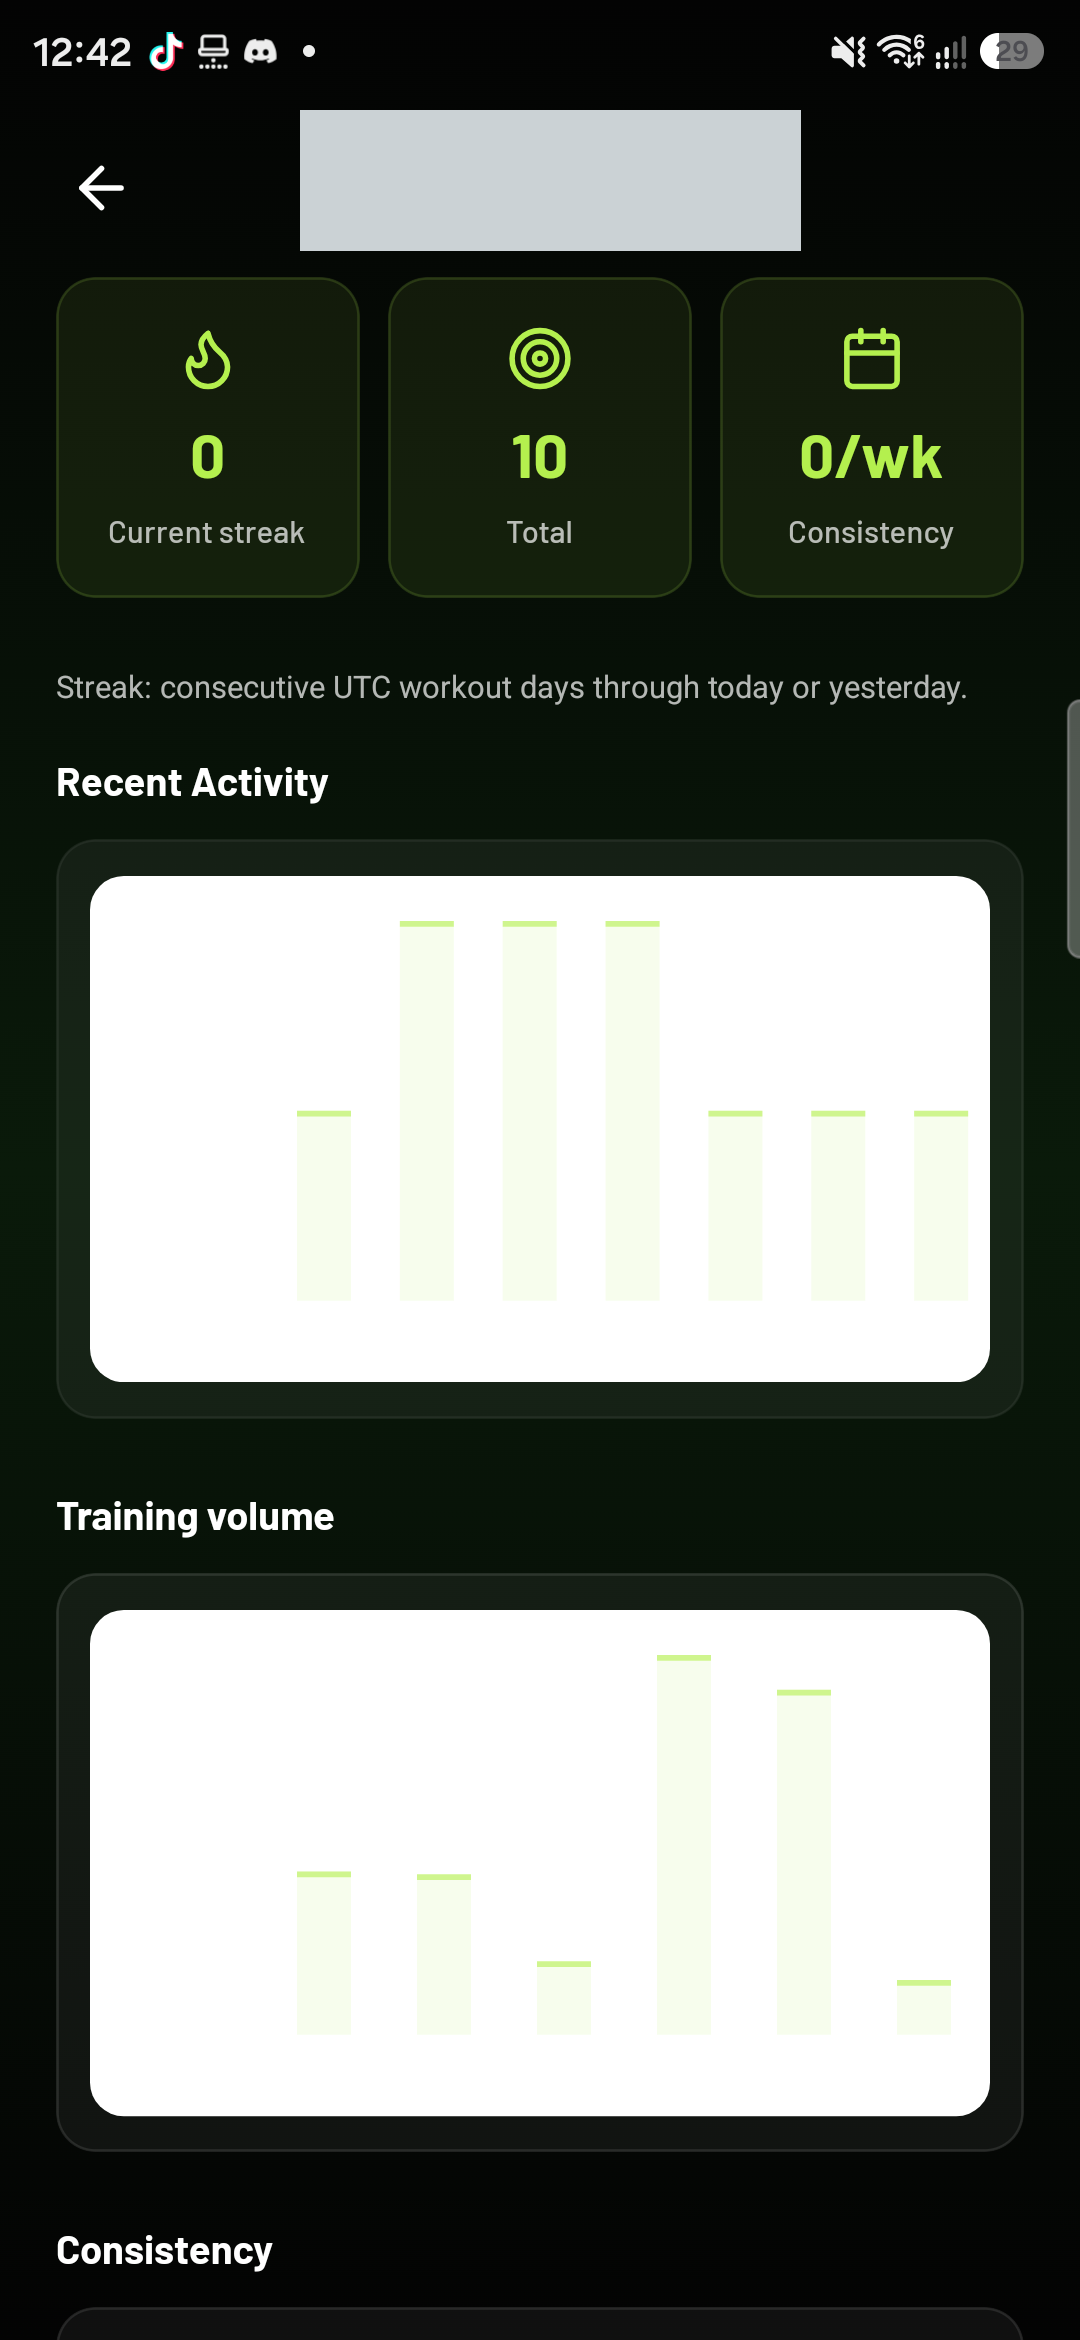
\includegraphics[width=\linewidth]{figures/screenshots/coach-client-progress.png}
\par\smallskip{\footnotesize b) Client progress view\par}
\end{minipage}
\hspace{0.025\linewidth}
\begin{minipage}[t]{.29\linewidth}
\centering
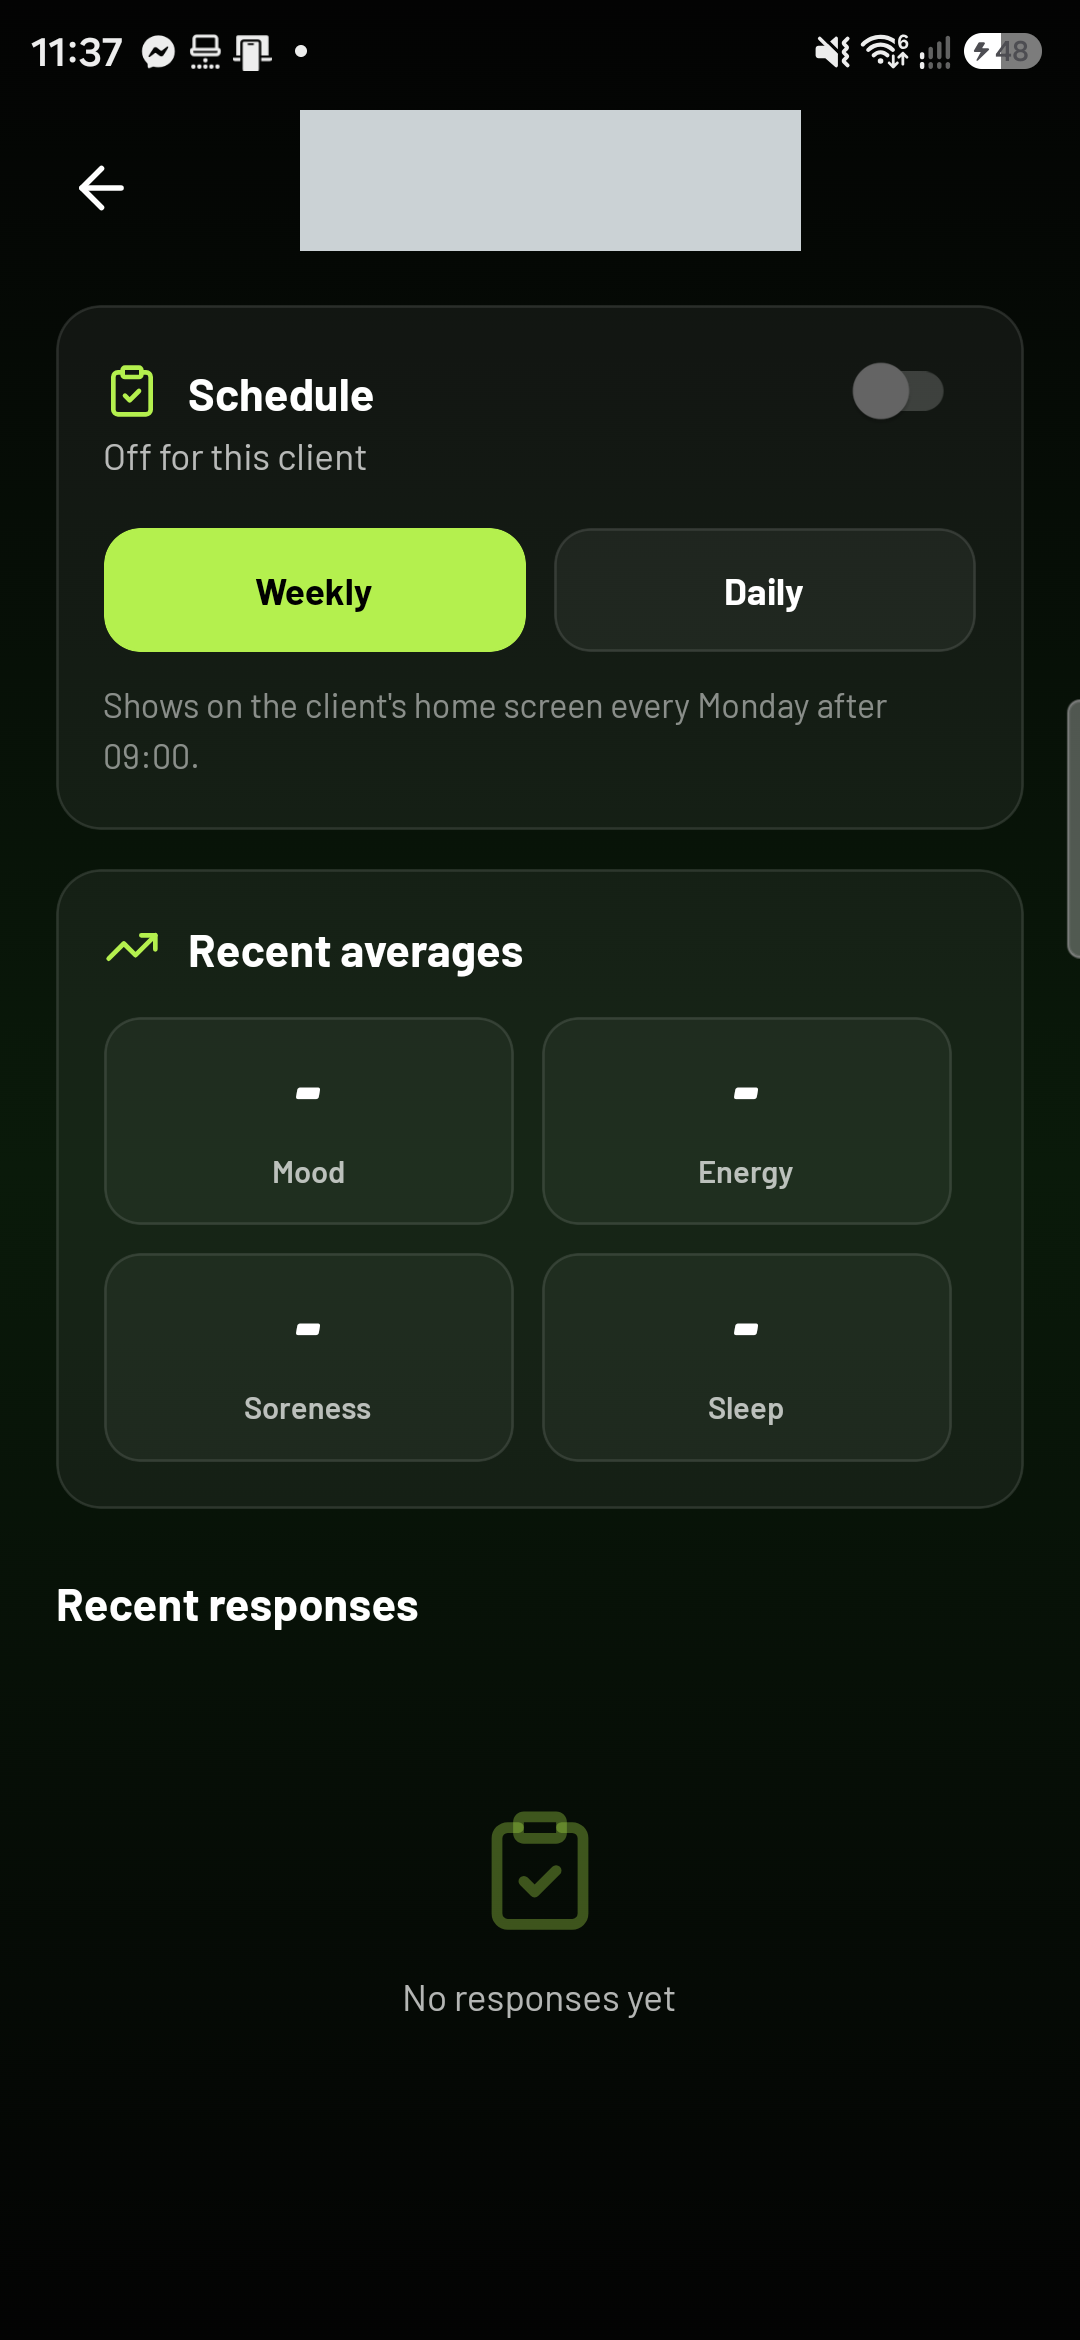
\includegraphics[width=\linewidth]{figures/screenshots/coach-checkin-schedule.png}
\par\smallskip{\footnotesize c) Check-in schedule and empty responses\par}
\end{minipage}
\caption{Coach interface walkthrough: dashboard, client progress and displayed check-in scheduling; client identifiers masked.}
\label{fig:ui-coach-followup-extended}
\end{figure}

\begin{figure}[H]
\centering
\begin{minipage}[t]{.29\linewidth}
\centering
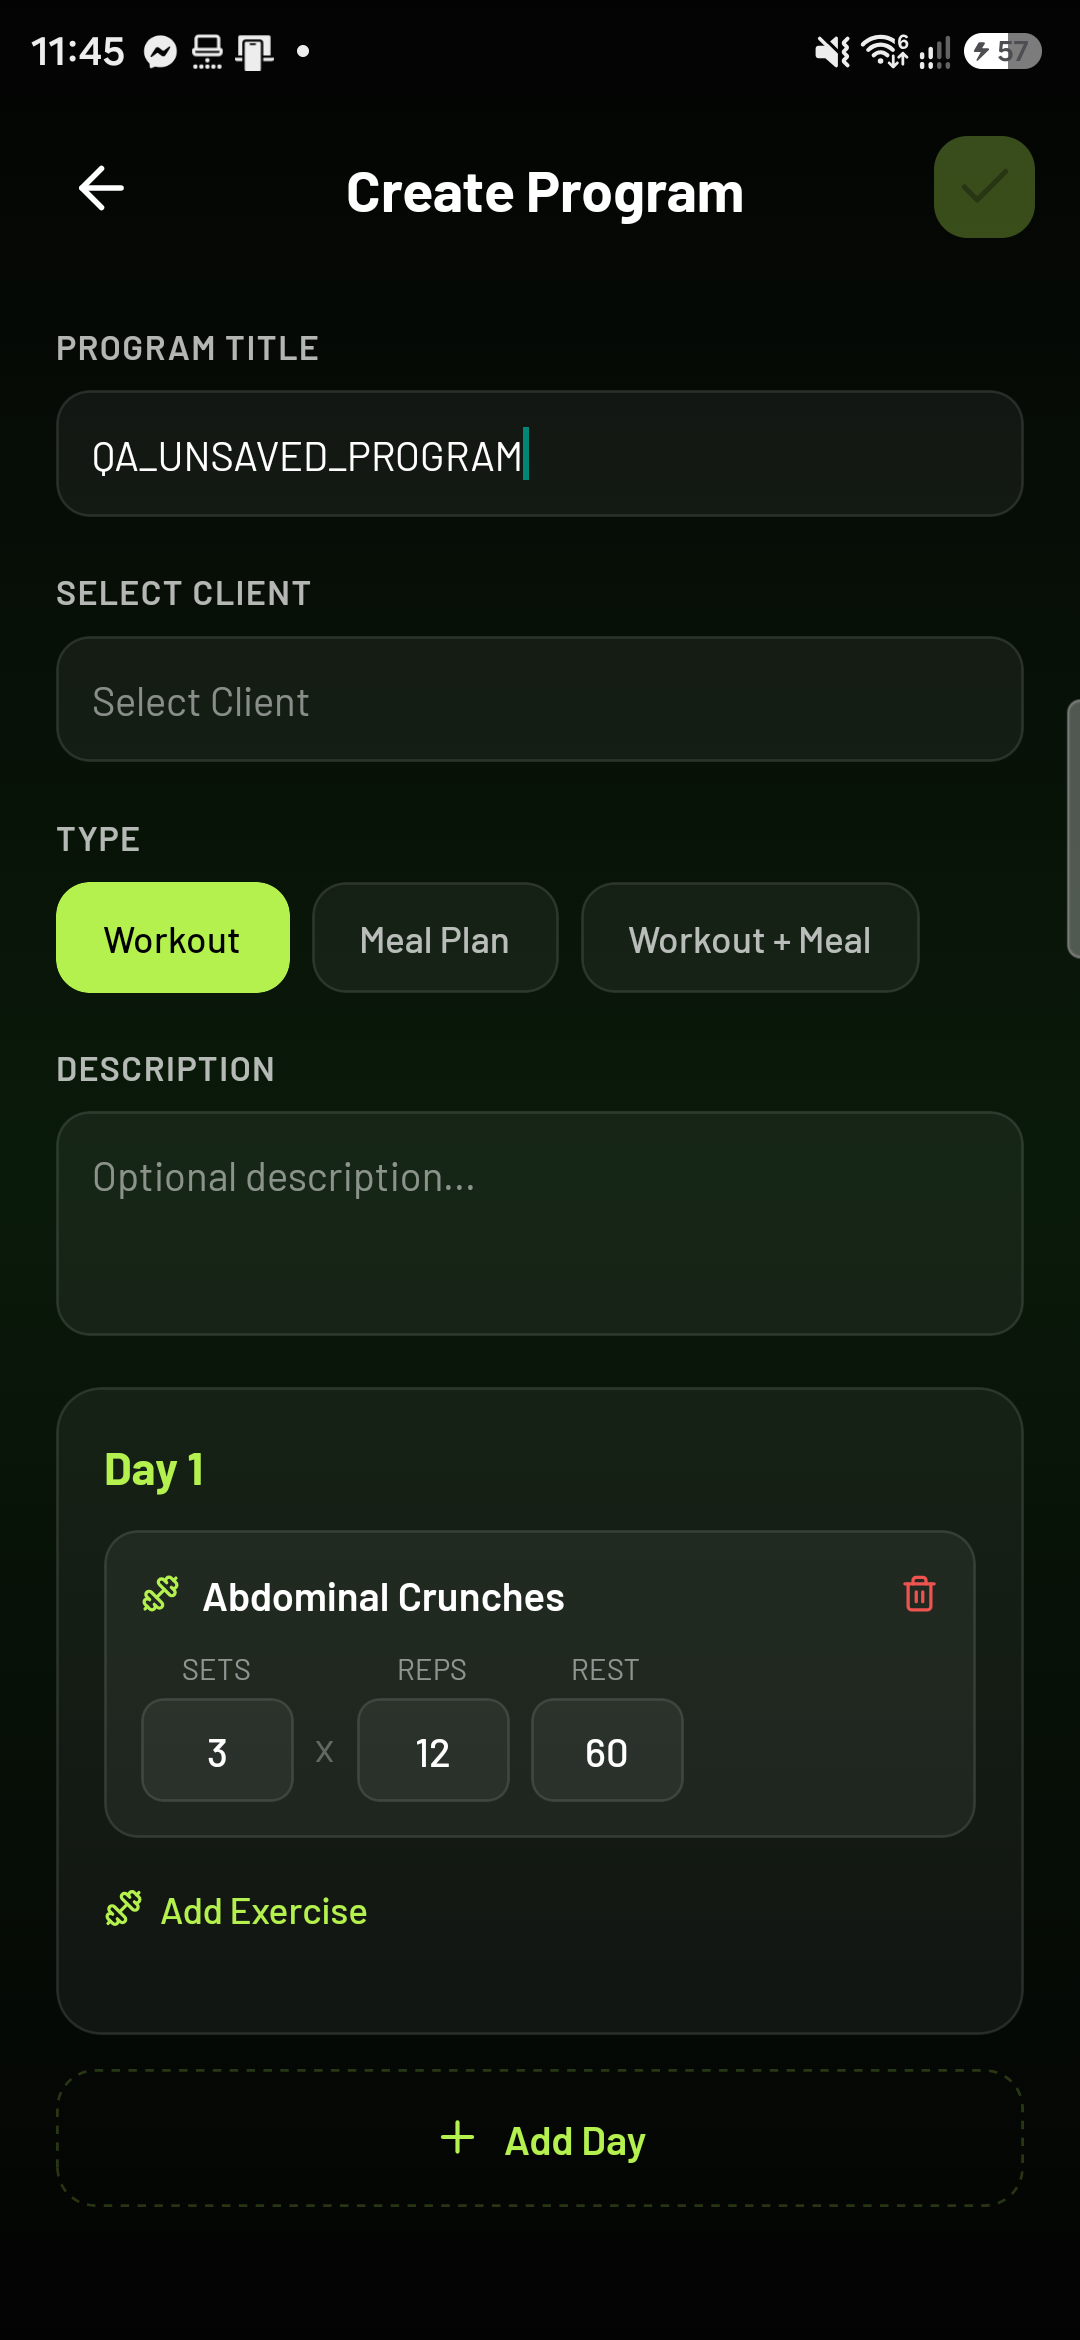
\includegraphics[width=\linewidth]{figures/screenshots/coach-configured-program-draft.png}
\par\smallskip{\footnotesize a) Unsubmitted program draft\par}
\end{minipage}
\hspace{0.025\linewidth}
\begin{minipage}[t]{.29\linewidth}
\centering
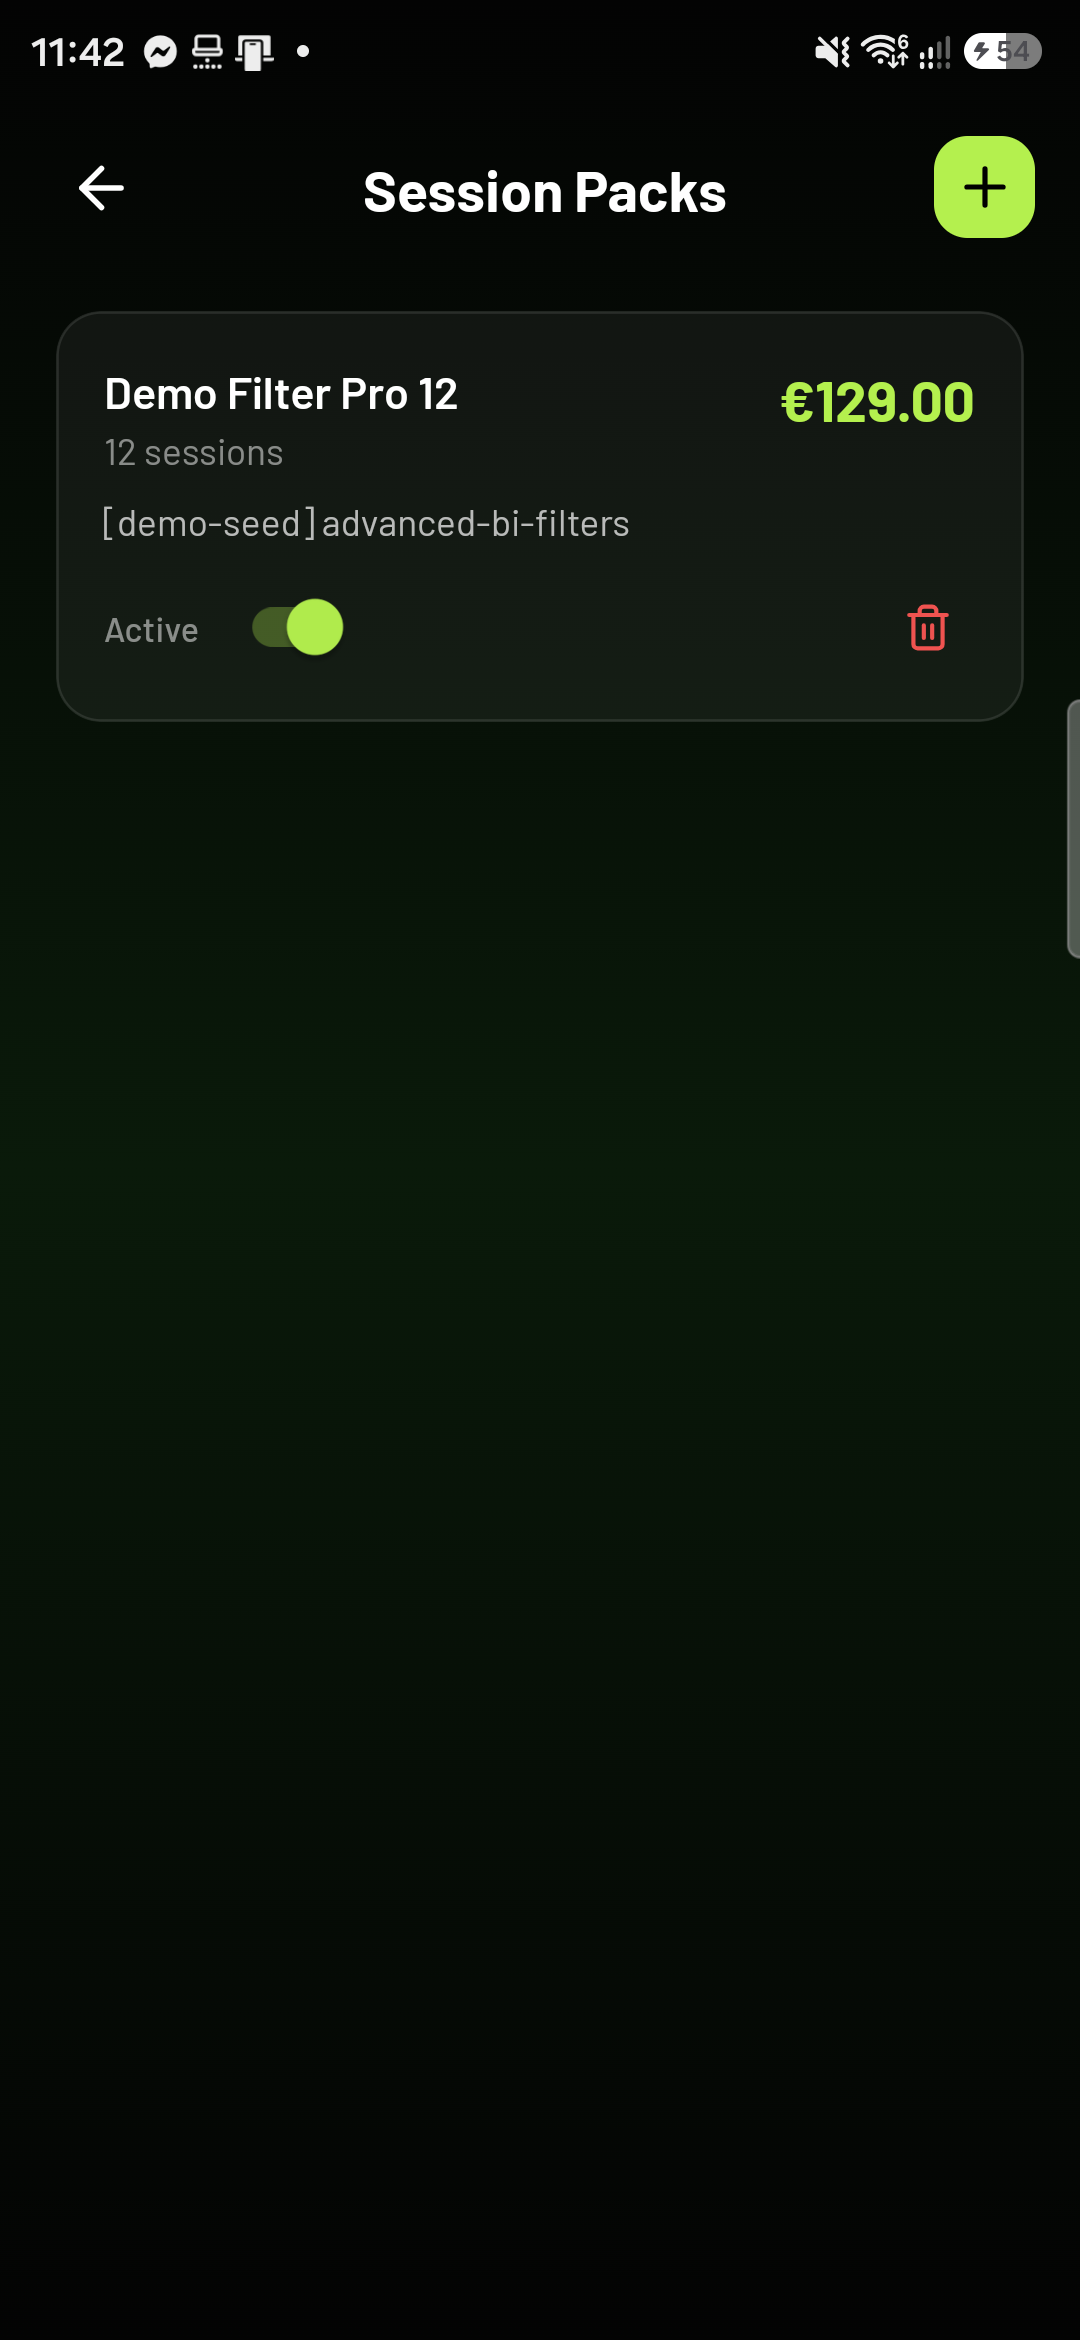
\includegraphics[width=\linewidth]{figures/screenshots/coach-pack-management.png}
\par\smallskip{\footnotesize b) Coach session-pack management\par}
\end{minipage}
\hspace{0.025\linewidth}
\begin{minipage}[t]{.29\linewidth}
\centering
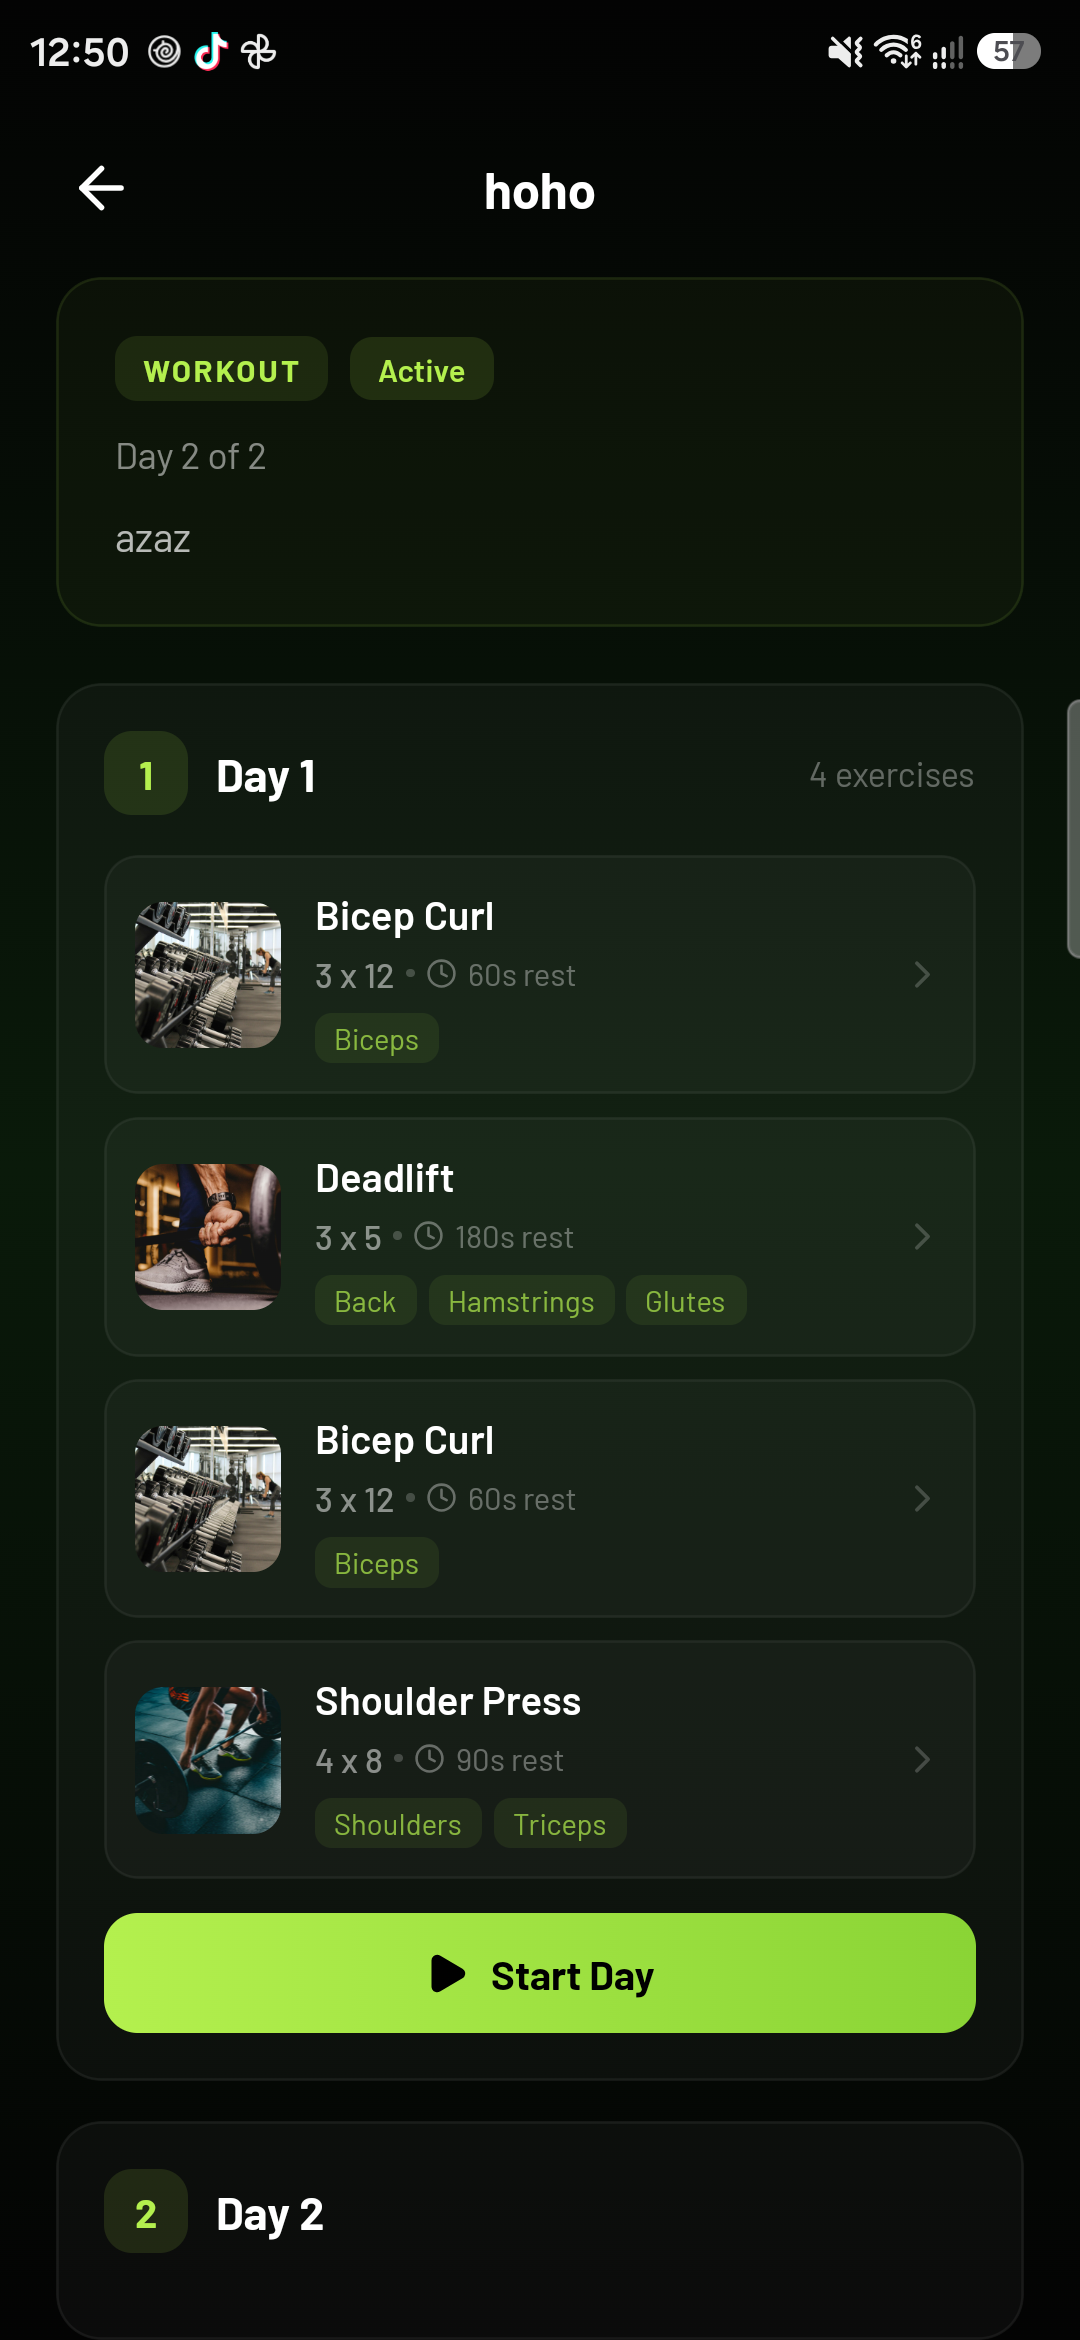
\includegraphics[width=\linewidth]{figures/screenshots/client-assigned-program-detail.png}
\par\smallskip{\footnotesize c) Existing assigned-program detail\par}
\end{minipage}
\caption{Coach/client program walkthrough: configured draft, session-pack offer and an existing assigned-program detail.}
\label{fig:ui-coach-program-pack}
\end{figure}

\subsection{Stripe Payment Integration and Persistence Boundaries}
\label{sec:current-payment-boundaries}

GoFit separates PaymentIntent creation from the mobile checkout interface. The Stripe secret key is read by the backend function, while the mobile client uses the returned client secret to initialize PaymentSheet. This separation describes the implemented integration and does not, by itself, establish payment compliance, settlement, or production readiness.


The corrected October implementation in \path{../supabase/functions/stripe-payment/index.ts} authenticates the caller in the handler and determines pack pricing from the active stored pack. Standalone session pricing uses the stored coach rate and duration in EUR, with server-side availability/reservation checks. Deployed function version 5 retains platform JWT verification disabled but requires a valid user through \texttt{getUser} and action-specific ownership checks in its handler. This differs from the earlier caller-priced USD baseline in the sequence figures.


The native sheet is only one stage. Pack fulfillment retrieves provider payment state and verifies owner, amount, currency and metadata before writing credits and the paid snapshot. Standalone sessions use reservation, card authorization, server capture and linked booking completion, with replay and overlap protection. One EUR129/12-credit pack was verified on Android; a separate EUR60/60-minute session was verified through provider/API/admin observations, with the native standalone flow still pending. The separate purchased-pack redemption branch must not be inferred to be an atomic part of this standalone flow.


These are synchronous sandbox scenarios, not a verified webhook/reconciliation system or a production payment certification. Same-reference retry is supported, but resumed-checkout recovery UI, scheduled reconciliation, refunds, payouts, 3DS/declines and iOS/release behavior remain incomplete or unverified. If capture or record completion is interrupted, recovery may require retry or operator review; an automatic refund must not be assumed. The retained payment evidence is identified in the final QA section.

Figure~\ref{fig:ui-sandbox-pack} illustrates the retained EUR129 pack sandbox checkout and success dialog. Figure~\ref{fig:ui-admin-paid-records} shows the matching administrative payment-state fields alongside the separate EUR60 standalone-session record. The latter was verified through API/provider checks, not a completed native standalone checkout.

\begin{figure}[H]
\centering
\begin{minipage}[t]{.31\linewidth}
\centering
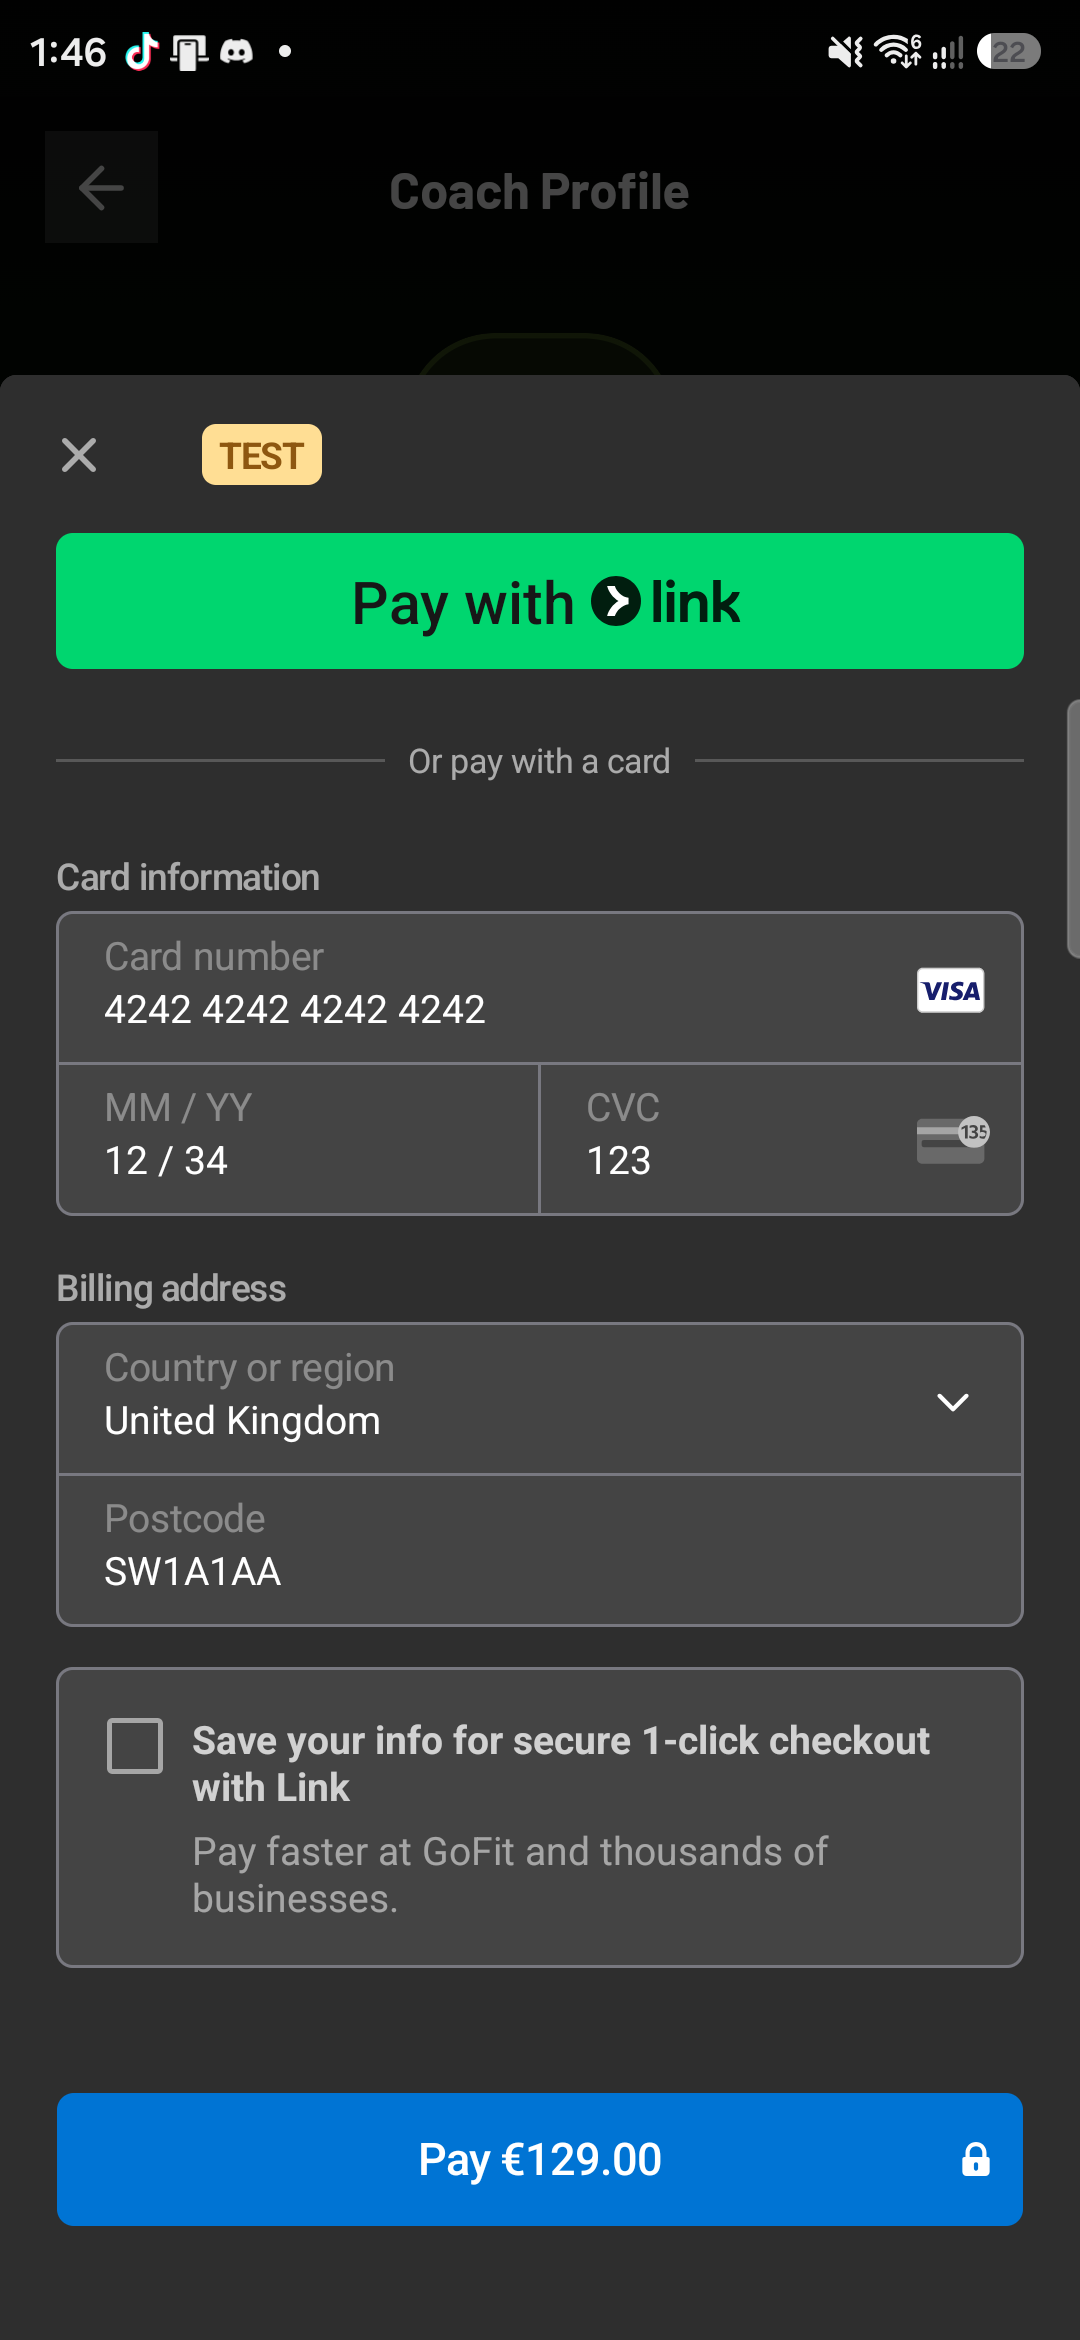
\includegraphics[width=\linewidth]{figures/screenshots/sandbox-eur-checkout.png}
\par\smallskip{\footnotesize a) Stripe test-mode checkout\par}
\end{minipage}
\hspace{0.025\linewidth}
\begin{minipage}[t]{.31\linewidth}
\centering
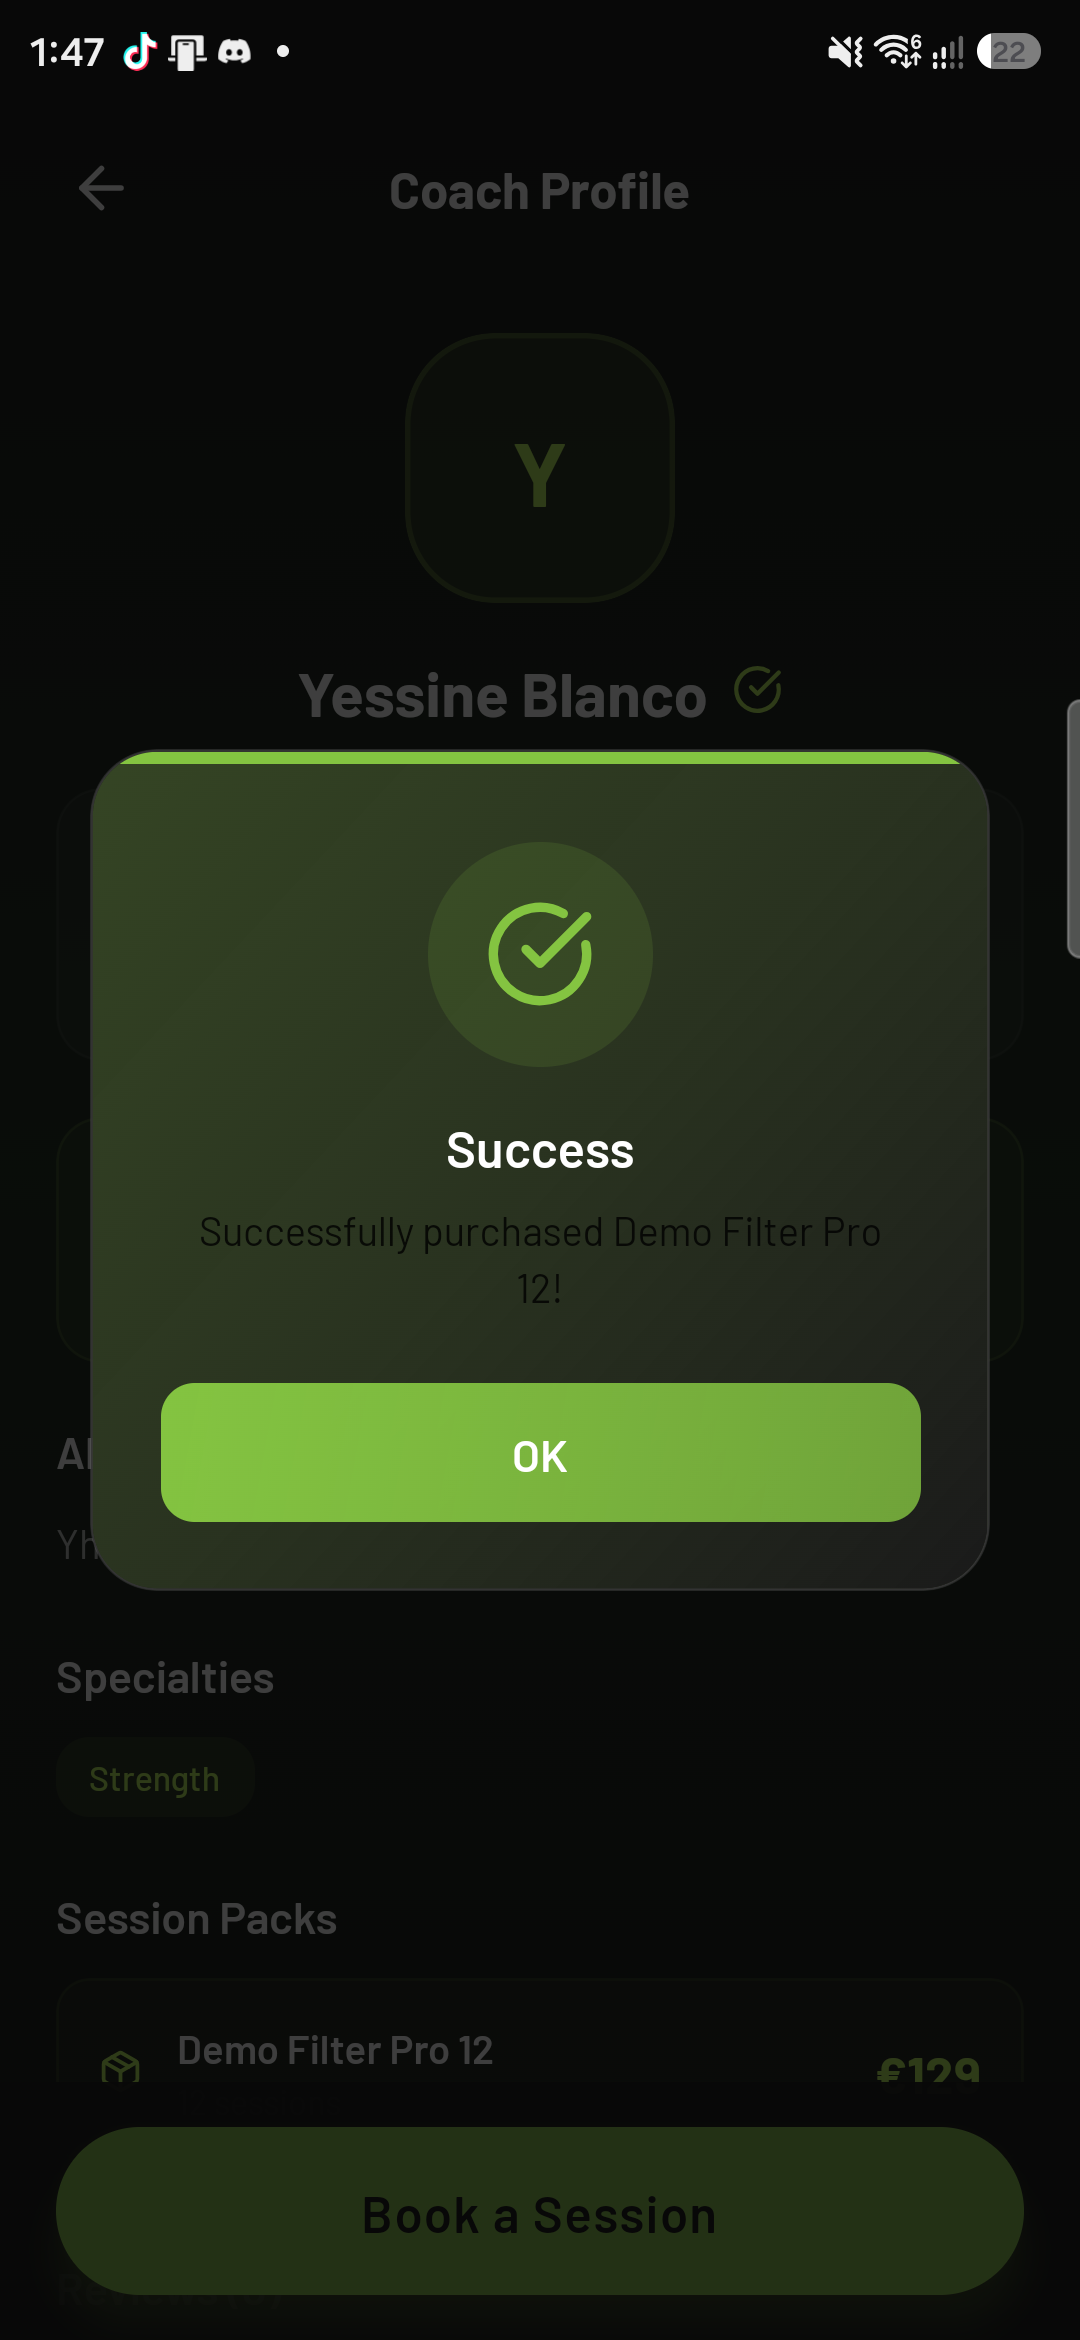
\includegraphics[width=\linewidth]{figures/screenshots/sandbox-pack-success.png}
\par\smallskip{\footnotesize b) Pack-purchase success dialog\par}
\end{minipage}
\caption{Sandbox interface captures: EUR129 test checkout and successful pack-purchase confirmation; no live charge is shown.}
\label{fig:ui-sandbox-pack}
\end{figure}

\begin{figure}[H]
\centering
\begin{minipage}[t]{.96\linewidth}
\centering
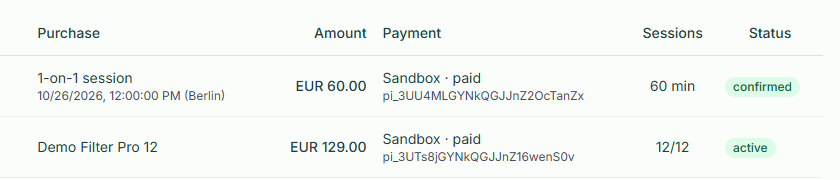
\includegraphics[width=\linewidth]{figures/screenshots/admin-sandbox-payment-records.png}

\end{minipage}
\caption{Administrative transaction excerpt: EUR60 standalone session and EUR129 pack marked sandbox-paid; identity columns omitted.}
\label{fig:ui-admin-paid-records}
\end{figure}

\subsection{Coach Check-in and Nutrition Context}

The coach workspace provides client context for fitness follow-up. Its check-in and nutrition views are support tools rather than clinically validated monitoring or medical decision systems.


The dashboard requests low check-in responses and provides client-navigation shortcuts; the source and empty-state query retest do not establish immediate alert delivery. Client Detail displays declared nutrition preferences, allergies and dislikes. Program-building checks can flag name matches against recorded preferences, but neither these checks nor the displayed profile establish complete allergen detection or clinical safety.


\subsection{High-Affordance Empty State Architecture}

A frequent source of user confusion in marketplace applications is unformatted or blank screens when no data exists (e.g., zero active clients, empty chat inbox, new wallet with zero transactions). GoFit introduces a centralized, modular EmptyState component across the coach application (ClientsListScreen, \seqsplit{ConversationsListScreen,} CoachWalletScreen). Each empty state renders contextual iconography, informative microcopy, and clear call-to-action buttons, guiding coaches and clients on immediate next steps.


Figure~\ref{fig:ui-conversation-empty} illustrates the coach conversation empty state. It is not evidence of a two-party message exchange or a connected video consultation; neither successful communication scenario is illustrated by the retained captures.

\begin{figure}[H]
\centering
\begin{minipage}[t]{.31\linewidth}
\centering
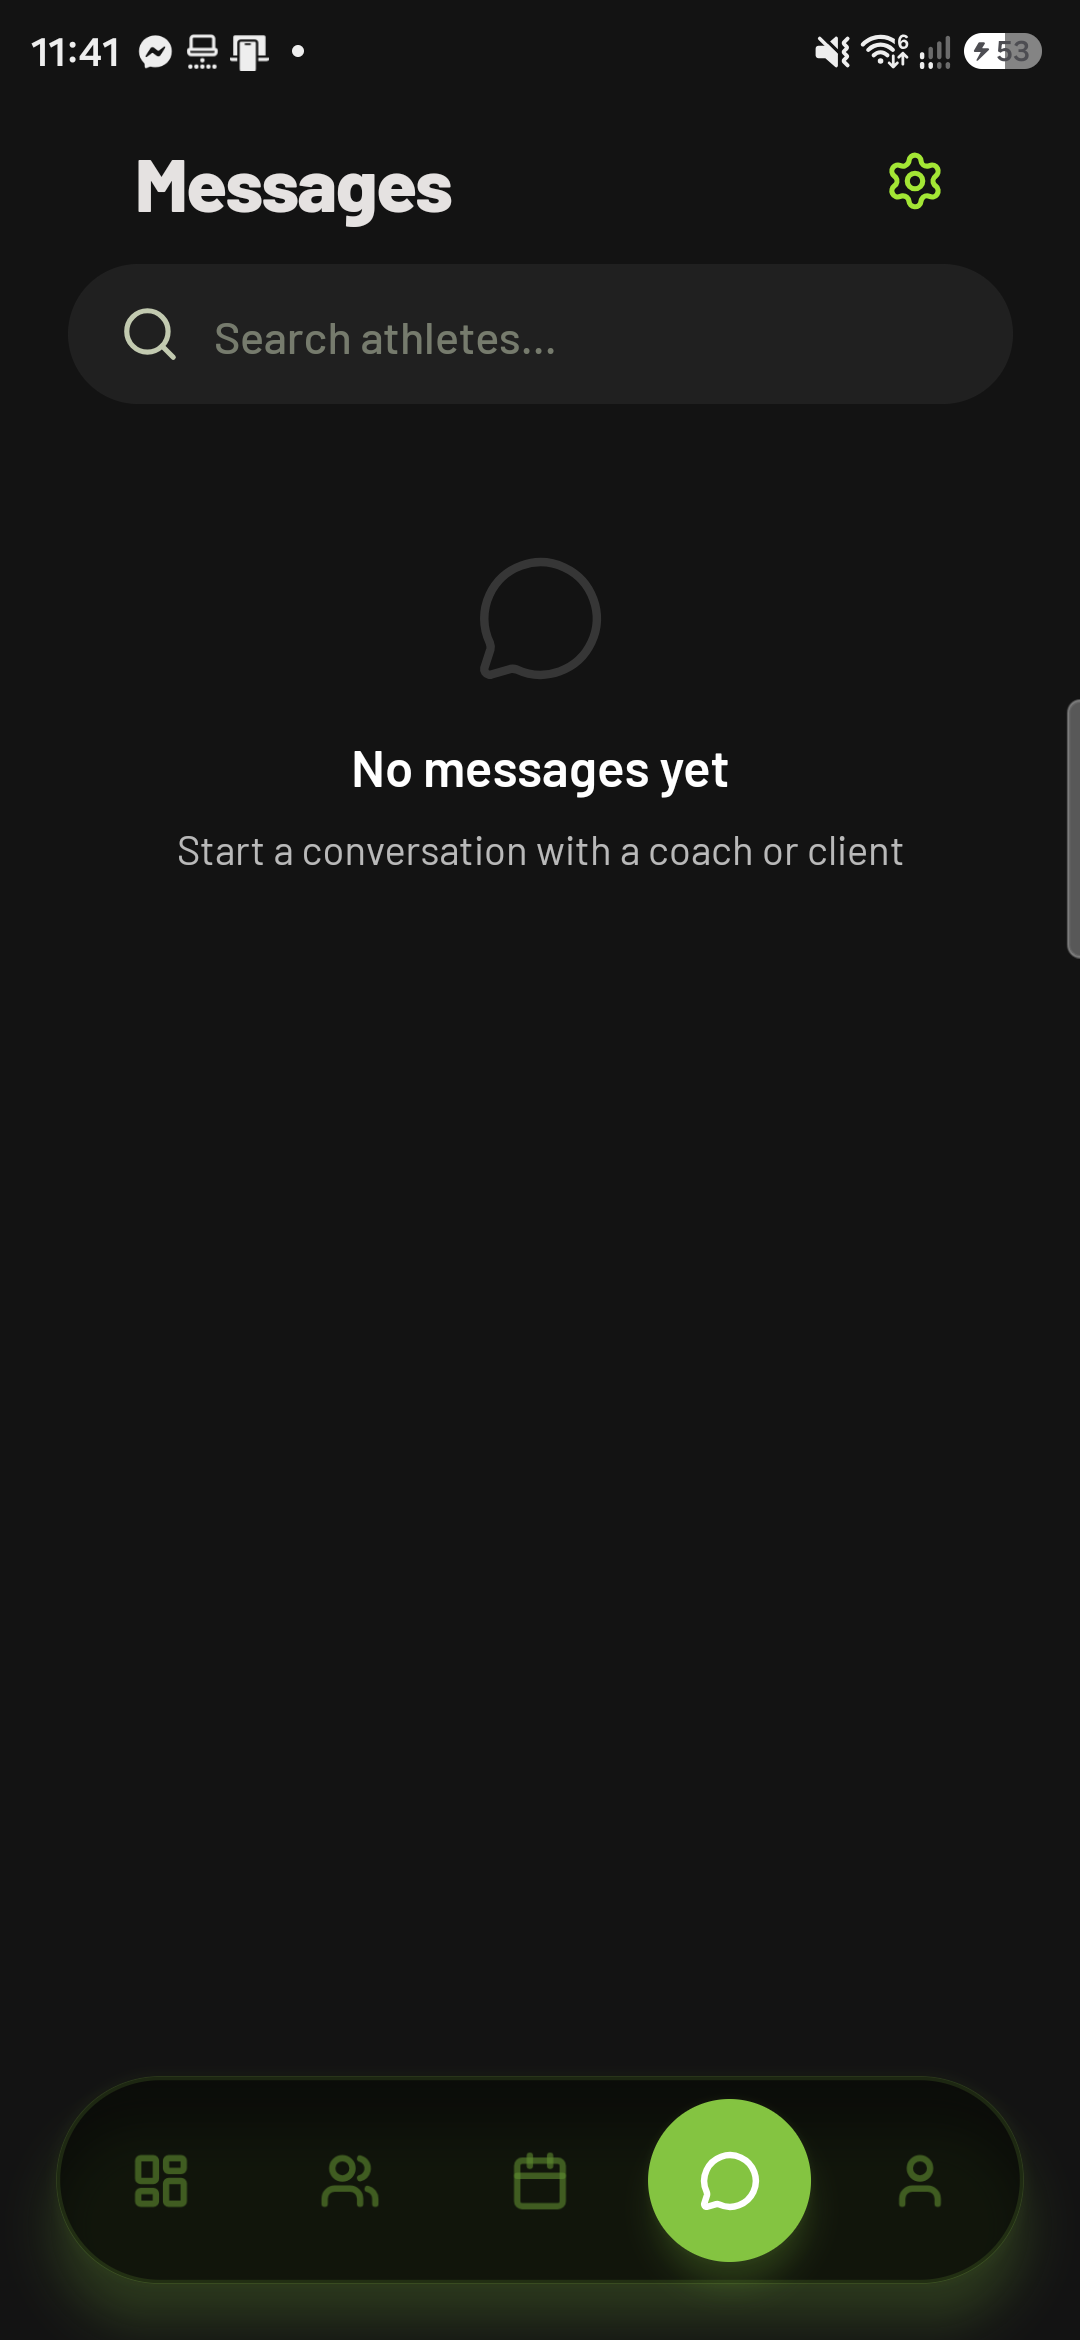
\includegraphics[width=\linewidth]{figures/screenshots/coach-message-empty-state.png}
\par\smallskip{\footnotesize a) Empty conversation list\par}
\end{minipage}
\caption{Interface capture: coach message-list empty state; successful messaging/video evidence remains pending.}
\label{fig:ui-conversation-empty}
\end{figure}

\subsection{Administration and Operational Control}

The administration panel is necessary because the platform contains user-generated data, coach applications, exercise content, workouts, transactions, notifications, and analytics. Without a back-office interface, the operator would need to manipulate database rows directly, which is risky and unsuitable for a production platform. The admin panel provides safer and more structured operational control.


The admin panel uses Next.js App Router and protected admin access. Server-side Supabase utilities are used for privileged operations, while middleware and admin-role checks prevent normal users from opening back-office pages. The design includes dashboard statistics, user management, coach validation, exercise/workout management, transaction review, notification management, settings, logs, analytics, search, and import/export foundations.


\begingroup
\footnotesize
\setlength{\tabcolsep}{3pt}
\renewcommand{\arraystretch}{1.20}
\setlength{\LTpre}{5pt}
\setlength{\LTpost}{10pt}
\begin{longtable}{|L{3.67cm}|L{5.29cm}|L{5.73cm}|}
\caption{Admin-panel operational modules}\label{tab:pdf-78-35} \\
\hline
Admin area & Managed data & Purpose \\ \hline
Dashboard & Users, exercises, workouts, sessions, transactions, coach status. & Provide a fast overview of platform health. \\ \hline
Users & Auth users and profile data. & Search, review, update, and monitor user accounts. \\ \hline
Coaches & Coach profiles, status, documents, marketplace visibility. & Validate coaches and maintain service quality. \\ \hline
Exercises and workouts & Exercise library, workout templates, metadata. & Maintain content consistency for mobile users. \\ \hline
Transactions and packs & Purchases, wallet/pack status, booking-related financial records. & Support marketplace operations and revenue visibility. \\ \hline
Notifications and logs & User notifications, admin activity, operational events. & Trace actions and communicate important updates. \\ \hline
Settings and analytics & Platform configuration and business indicators. & Prepare the product for scaling and decision-making. \\ \hline
\end{longtable}
\endgroup

\subsubsection{Administration Panel: Interface Walkthrough}
\label{sec:admin-panel-screens}

The following browser captures belong to the Next.js administration panel, not the mobile application. The walkthrough begins with the dashboard and continues through user management, coach management, catalog editing and operational records. Captures are from the local October QA environment; identifiers are masked in the user and coach lists. User-account and profile counts describe different populations and must not be conflated.

\begin{figure}[H]
\centering
\begin{minipage}[t]{.96\linewidth}
\centering
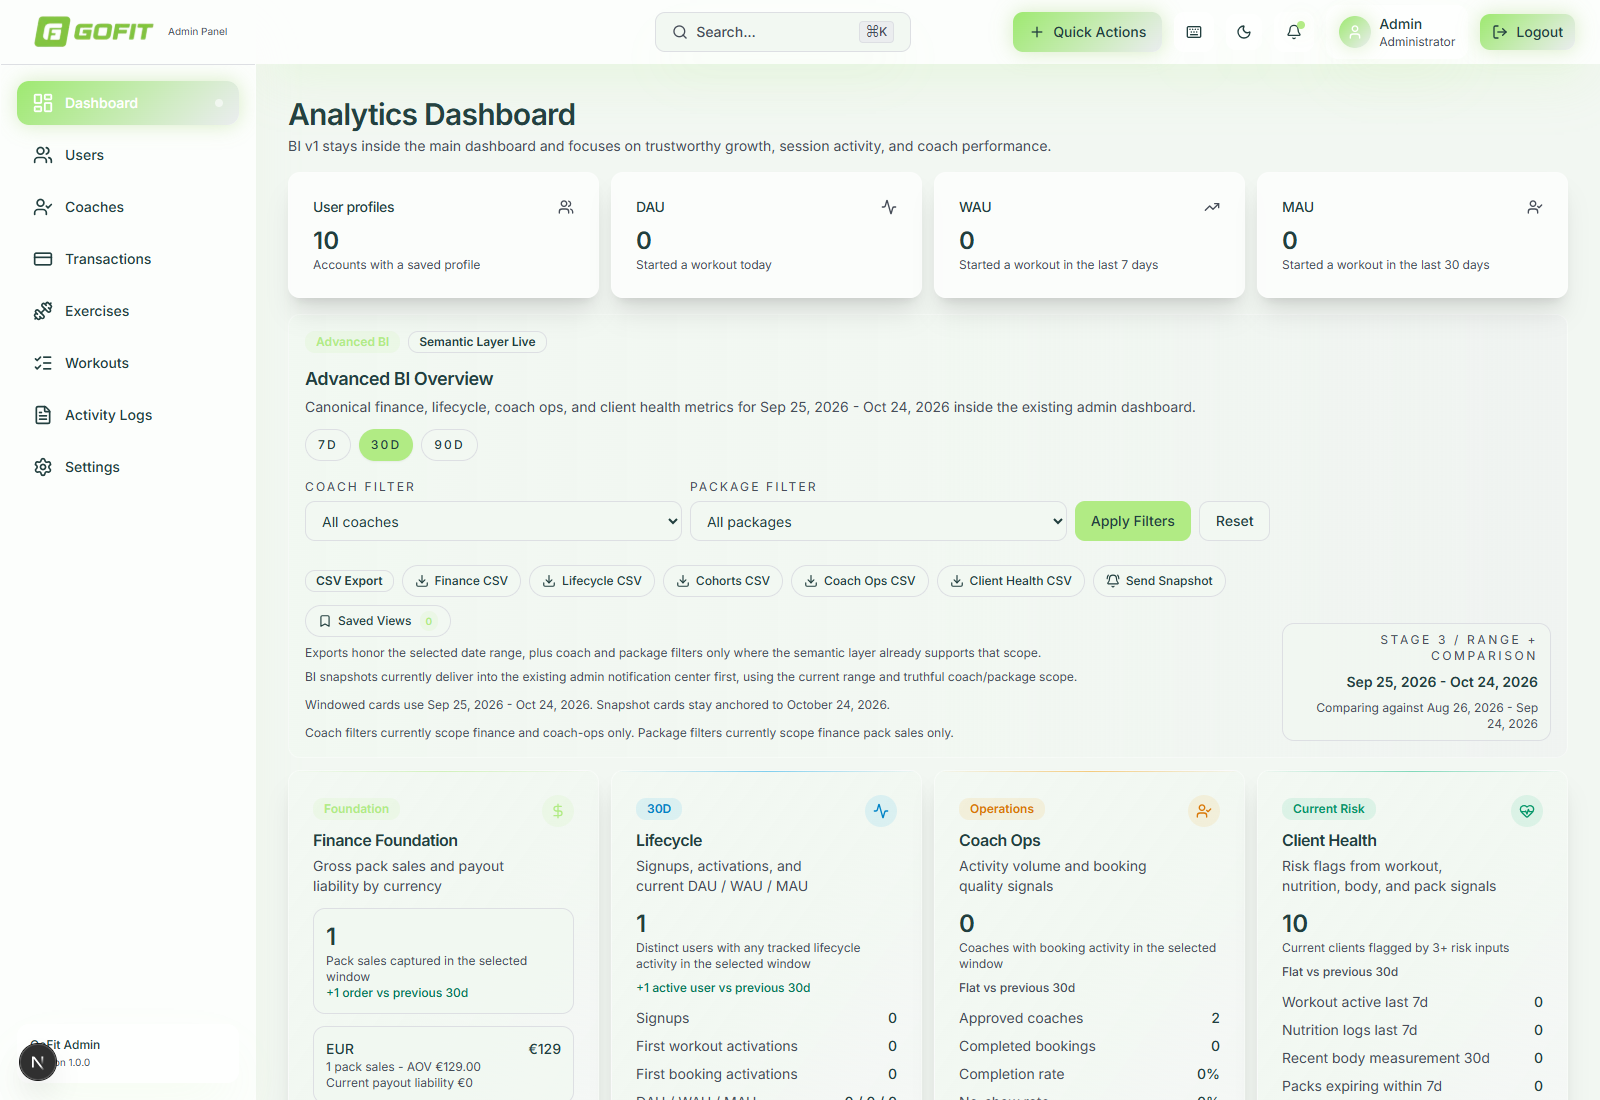
\includegraphics[width=\linewidth]{figures/screenshots/admin-dashboard.png}

\end{minipage}
\caption{Administrative dashboard capture: user-profile count and operational BI overview after the label correction.}
\label{fig:ui-admin-dashboard}
\end{figure}

\begin{figure}[H]
\centering
\begin{minipage}[t]{.98\linewidth}
\centering
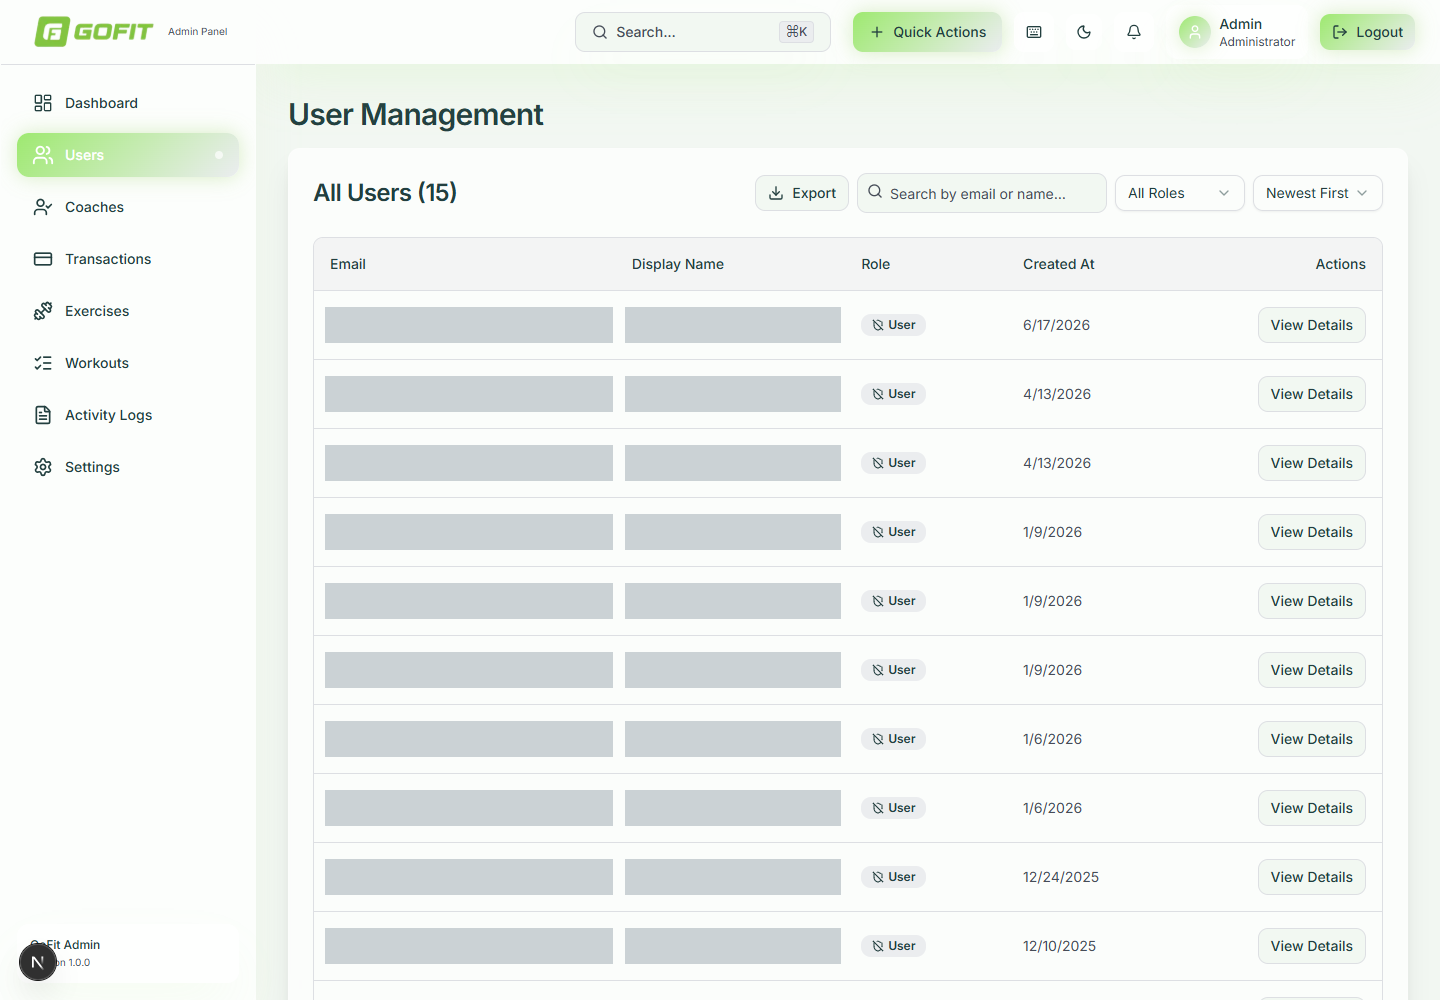
\includegraphics[width=\linewidth]{figures/screenshots/admin-user-management-masked.png}

\end{minipage}
\caption{Administration panel: user-account management, role filters and record actions; names and emails masked for the report.}
\label{fig:ui-admin-users}
\end{figure}

\begin{figure}[H]
\centering
\begin{minipage}[t]{.98\linewidth}
\centering
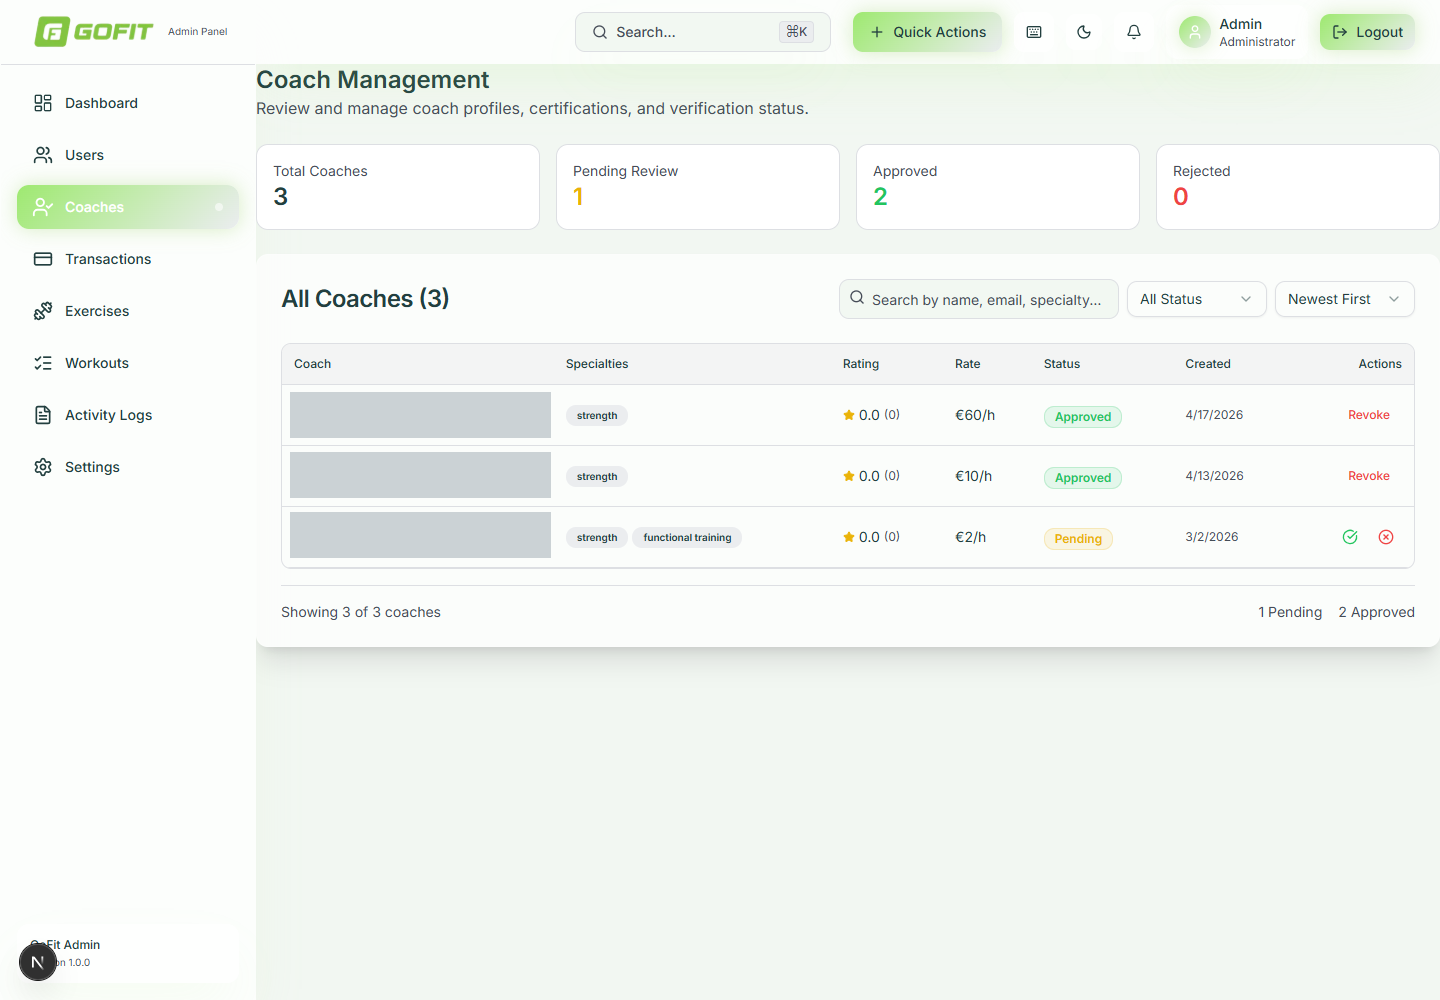
\includegraphics[width=\linewidth]{figures/screenshots/admin-coach-management-masked.png}

\end{minipage}
\caption{Administration panel: coach-profile review, status filters and decision controls; personal identifiers masked.}
\label{fig:ui-admin-coaches}
\end{figure}

Figures~\ref{fig:ui-admin-exercises} and~\ref{fig:ui-admin-workout} illustrate catalog management and a reloaded disposable workout fixture. Figure~\ref{fig:ui-admin-approval-audit} separates an approval confirmation dialog from exercise-deletion audit records. The coach-approval action was cancelled in the retained test; the audit excerpt concerns exercise deletion and does not establish approval auditing.

\begin{figure}[H]
\centering
\begin{minipage}[t]{.96\linewidth}
\centering
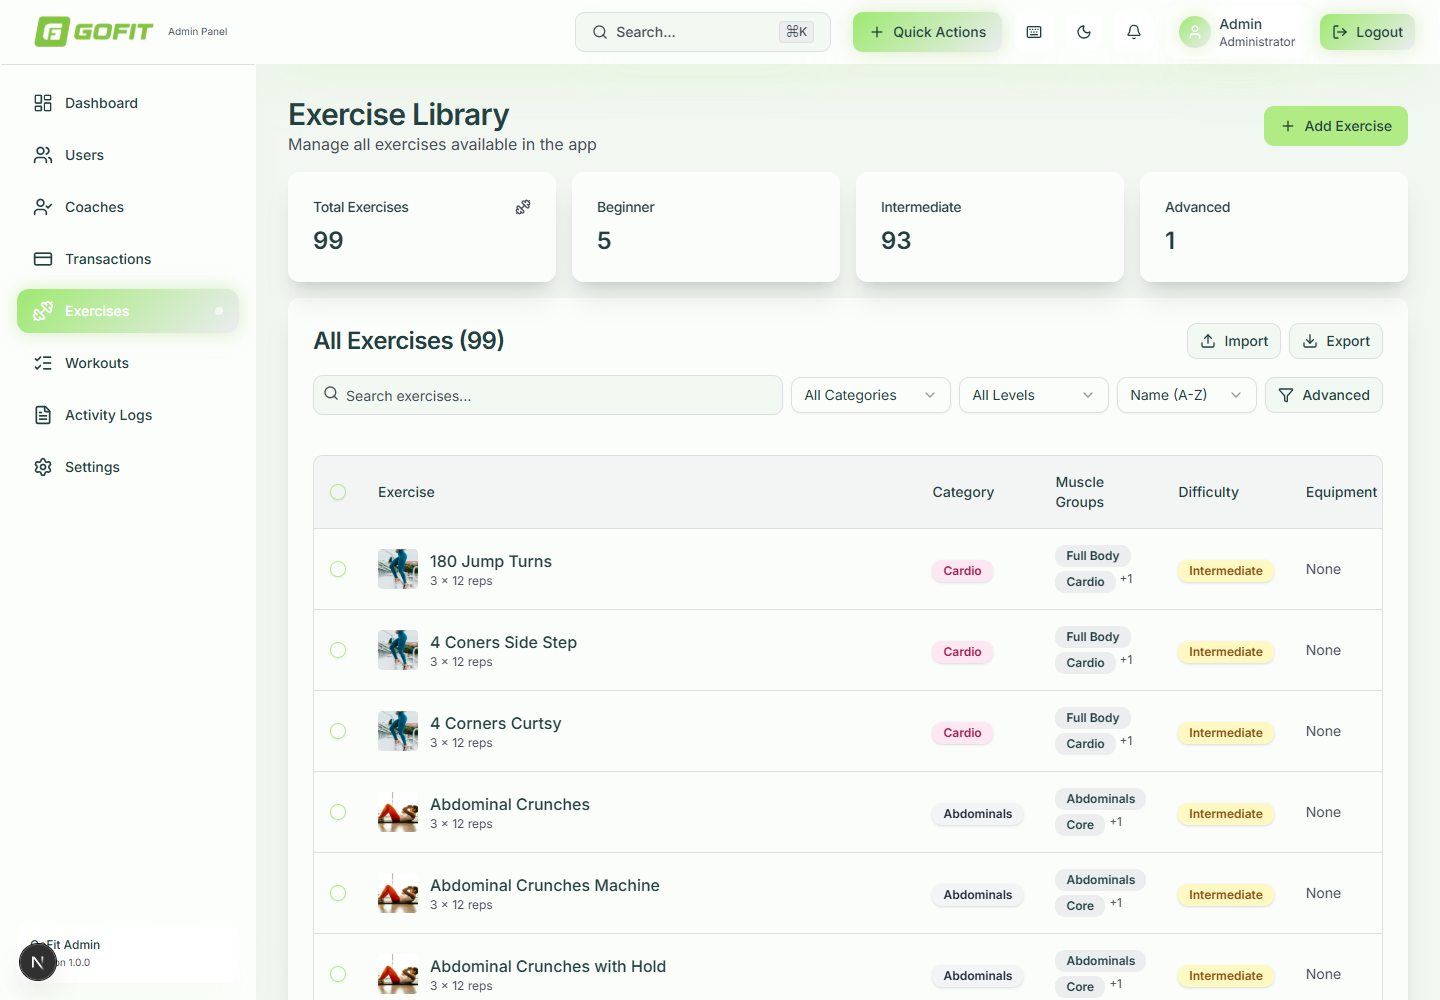
\includegraphics[width=\linewidth]{figures/screenshots/admin-exercise-catalog.png}

\end{minipage}
\caption{Administrative interface: exercise catalog, search/filter controls and management actions in the local QA environment.}
\label{fig:ui-admin-exercises}
\end{figure}

\begin{figure}[H]
\centering
\begin{minipage}[t]{.96\linewidth}
\centering
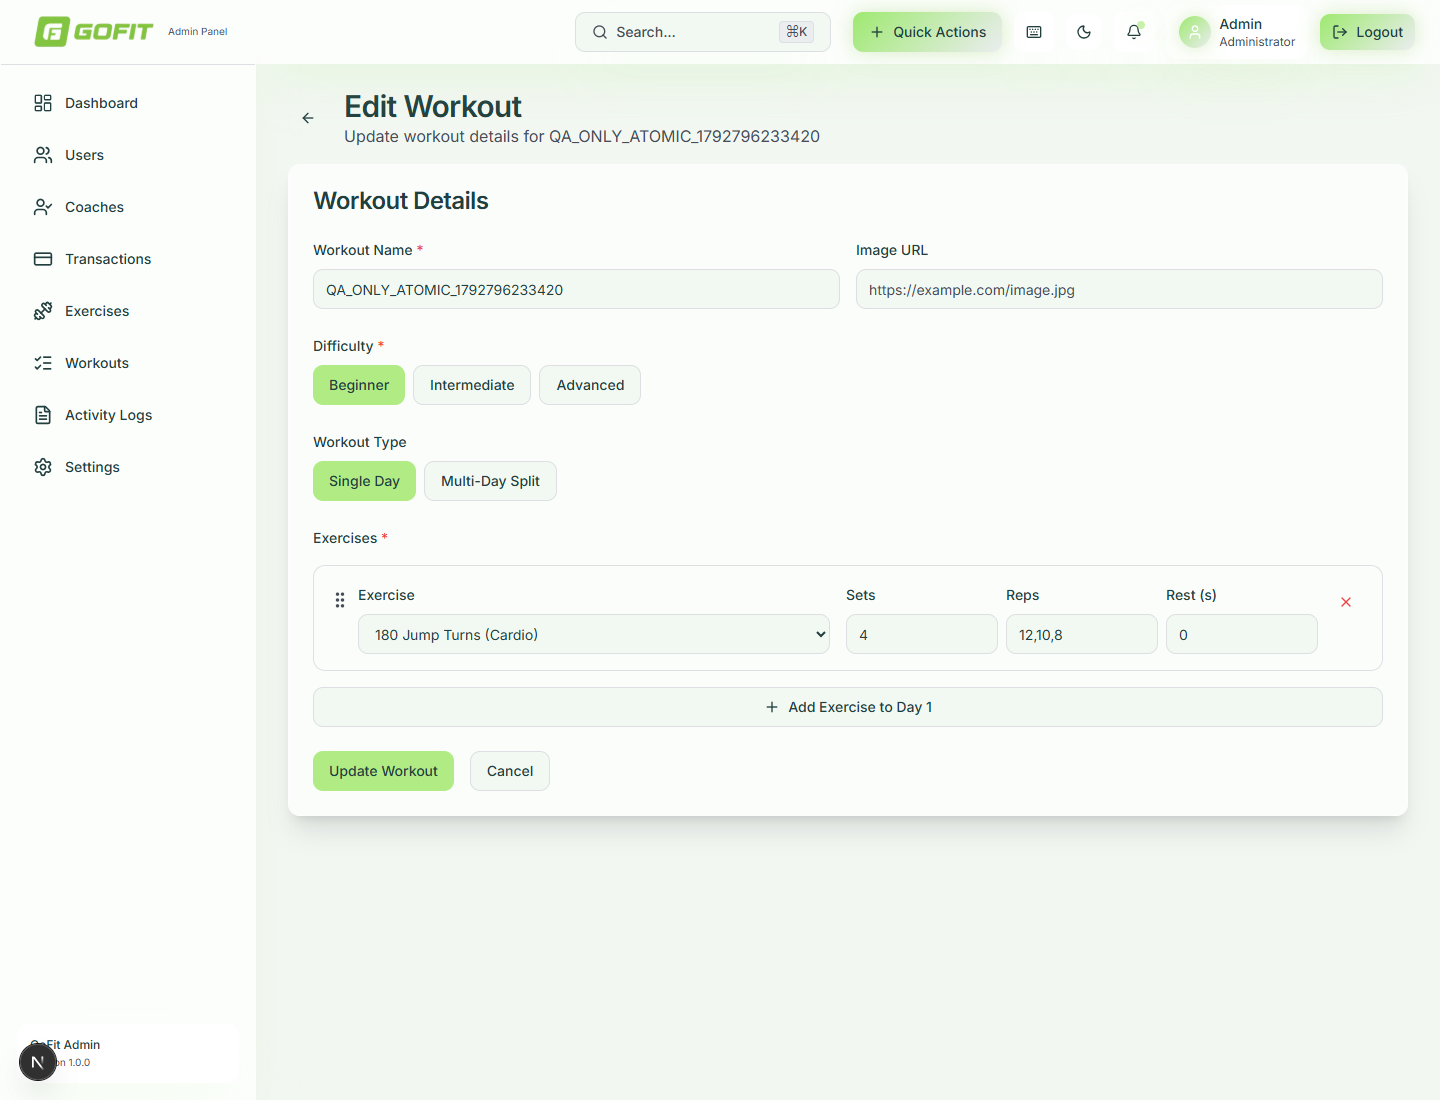
\includegraphics[width=\linewidth]{figures/screenshots/admin-disposable-workout-editor.png}

\end{minipage}
\caption{Administrative interface: disposable workout fixture reopened after editing; this test record was subsequently removed.}
\label{fig:ui-admin-workout}
\end{figure}

\begin{figure}[H]
\centering
\begin{minipage}[t]{.96\linewidth}
\centering
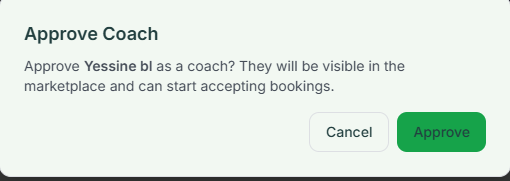
\includegraphics[width=\linewidth]{figures/screenshots/admin-approval-dialog.png}
\par\smallskip{\footnotesize a) Approval confirmation dialog\par}
\end{minipage}
\par\medskip
\begin{minipage}[t]{.96\linewidth}
\centering
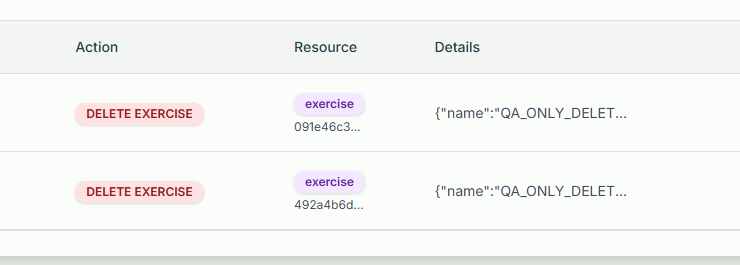
\includegraphics[width=\linewidth]{figures/screenshots/admin-exercise-audit-excerpt.png}
\par\smallskip{\footnotesize b) Exercise-deletion audit excerpt\par}
\end{minipage}
\caption{Administrative excerpts: coach-approval confirmation (cancelled) and exercise-deletion audit entries; unrelated identity/network columns omitted.}
\label{fig:ui-admin-approval-audit}
\end{figure}

Figures~\ref{fig:ui-admin-saved-view} and~\ref{fig:ui-admin-settings-summary} complete the web walkthrough with a disposable saved-view configuration and the corrected profile-count summary. The verified sandbox transaction excerpt remains in Figure~\ref{fig:ui-admin-paid-records}; it is a browser view, not another mobile screen.

\begin{figure}[H]
\centering
\begin{minipage}[t]{.98\linewidth}
\centering
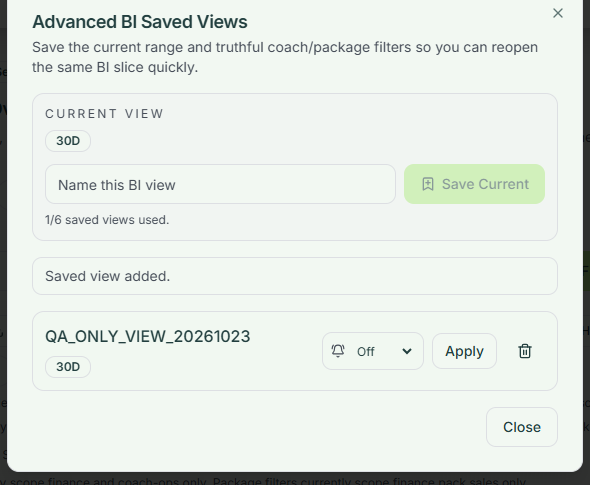
\includegraphics[width=\linewidth]{figures/screenshots/admin-saved-view-dialog.png}

\end{minipage}
\caption{Administration panel: disposable saved BI view shown in its dialog; the QA view was subsequently removed.}
\label{fig:ui-admin-saved-view}
\end{figure}

\begin{figure}[H]
\centering
\begin{minipage}[t]{.98\linewidth}
\centering
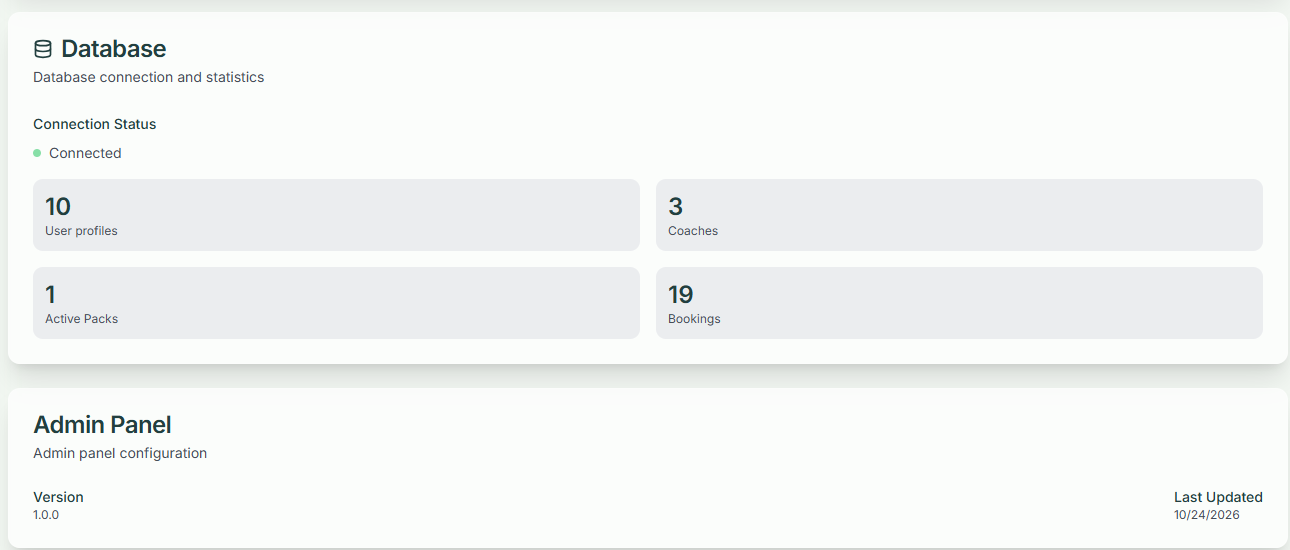
\includegraphics[width=\linewidth]{figures/screenshots/admin-database-summary.png}

\end{minipage}
\caption{Administration panel: settings-page database summary, including the corrected user-profile label; captured totals belong to the QA environment.}
\label{fig:ui-admin-settings-summary}
\end{figure}

\subsection{Admin Analytics and Business Intelligence Features}

The administration panel also includes a business intelligence dimension. This work is more than a simple dashboard counter: it transforms operational data from users, workouts, bookings, coaches, session packs, finance records, and health/readiness signals into indicators that an administrator can use


for monitoring and decision-making. The BI area is implemented inside the main dashboard so that operational control and performance interpretation stay in the same protected back-office interface.


The first analytics layer provides platform visibility: registered users, daily/weekly/monthly active users, user growth, popular exercises, workout completion rates, activity heatmaps, session activity, and recent activity. The advanced BI layer adds deeper decision-support views: finance by currency and coach/package scope, user lifecycle and activation signals, workout cohort retention, coach operations, client health risk queues, threshold alerts, saved BI views, snapshot notifications, scheduled digests, and CSV exports.


\begingroup
\footnotesize
\setlength{\tabcolsep}{3pt}
\renewcommand{\arraystretch}{1.20}
\setlength{\LTpre}{5pt}
\setlength{\LTpost}{10pt}
\begin{longtable}{|L{3.67cm}|L{5.29cm}|L{5.73cm}|}
\caption{Admin analytics and BI dashboard features}\label{tab:pdf-79-36} \\
\hline
BI feature & Source/implementation & Administrative value \\ \hline
Engagement metrics & \seqsplit{admin-panel/lib/analytics.ts;} \seqsplit{EngagementMetricsCards;} workout sessions and user profiles. \_ \_ & Tracks total users, DAU, WAU, and MAU to measure platform activity. \\ \hline
User growth chart & UserGrowthChart;user profiles.created at grouped by \_ \_ date. & Shows acquisition trend and cumulative user growth. \\ \hline
Popular exercises & PopularExercisesCard; exercises joined with workout exercises usage \_ counts. & Identifies content that is most used by members. \\ \hline
Workout completion and session activity & WorkoutCompletionCard and SessionActivityChart; workout sessions. \_ & Detects completion rate, training volume, and possible workout drop-off. \\ \hline
Activity heatmap and recent activity & ActivityHeatmap and RecentActivityFeed; completed sessions and activity records. & Shows when users are active and what happened recently on the platform. \\ \hline
Advanced BI overview & \seqsplit{admin-panel/app/dashboard/page.tsx} with bi-finance, bi-user-lifecycle, bi-coach-ops, and bi-client-health services. & Combines finance, lifecycle, coach operations, and client health into one decision panel. \\ \hline
Threshold alerts & BIThresholdAlertsCard with client-health rows. & Highlights users with risk signals so administrators can notice operational issues earlier. \\ \hline
Saved BI views & AdvancedBISavedViews and /api/bi/saved-views. & Allows administrators to save BIfilter/range configurations and digest cadence. \\ \hline
BI snapshots and scheduled digests & \seqsplit{AdvancedBISnapshotButton,} /api/bi/snapshot, and \seqsplit{/api/bi/scheduled-digests.} & Creates admin notification summaries on demand or according to saved-view cadence. \\ \hline
CSV exports & /api/bi/export with finance, lifecycle, cohort, coach-ops, and client-health slices. & Lets administrators extract BI data for external reporting or academic evidence. \\ \hline
\end{longtable}
\endgroup

\begingroup
\scriptsize
\setlength{\tabcolsep}{3pt}
\renewcommand{\arraystretch}{1.20}
\setlength{\LTpre}{5pt}
\setlength{\LTpost}{10pt}
\begin{longtable}{|L{2.74cm}|L{5.18cm}|L{4.18cm}|L{2.30cm}|}
\caption{Advanced BI data domains and limits}\label{tab:pdf-80-37} \\
\hline
\rowcolor{entetetab}
Domain & Database/service evidence & Metrics covered & Known limit in v1 \\ \hline
\endfirsthead
\hline
\rowcolor{entetetab}
Domain & Database/service evidence & Metrics covered & Known limit in v1 \\ \hline
\endhead
Finance & bi finance daily view; \_ \_ \seqsplit{admin-panel/lib/bi-finance.ts;} \seqsplit{FinanceCurrencyDetailCar} d. & Gross pack sales, pack count, ledger signals, currency summaries, coach/package filters. & Net revenue, refunds, payout reconciliation, and full accounting remain deferred. \\ \hline
User lifecycle & bi user lifecycle daily \_ \_ \_ view; \seqsplit{admin-panel/lib/bi-user-lifecycle.ts;} \seqsplit{LifecycleActivationDetailCa} rd. & Signup, first workout activation, first booking activation, activity windows, DAU/WAU/MAU. & Coach filters do not scope lifecycle cohorts in v1; lifecycle may include non-client profiles where relevant. \\ \hline
Workout cohort retention & bi-user-lifecycle cohort helper; RetentionCohortCard. & Signup-to-workout retention by cohort period. & Cohorts depend on available historical workout data. \\ \hline
Coach operations & bi coach ops daily view; \_ \_ \_ \seqsplit{admin-panel/lib/bi-coach-ops.ts;} CoachOpsDetailCard and CoachPerformanceTable. & Booking activity, completion rate, cancellation/no-show signals, coach activity, package context. & Coach filters scope coach operations, but not every dashboard card is coach-scoped. \\ \hline
Client health & bi client health daily \_ \_ \_ view; \seqsplit{admin-panel/lib/bi-client-health.ts;} \seqsplit{ClientHealthRiskQueueand} \seqsplit{ClientHealthTrendDetailCa} rd. & Inactive clients, nutrition gaps, body-measurement gaps, pack/session risk signals, aggregated risk counts. & Risk indicators are operational signals, not medical diagnosis. \\ \hline
Security and access & fix bi views security invo \_ \_ \_ \_ ker.sql; admin middleware; server-side Supabase utilities. & Admin-only dashboard and BI API access with protected routes. & Final QA must still attach admin/\allowbreak non-admin access screenshots and API test outputs. \\ \hline
\end{longtable}
\endgroup

This BI layer is important academically because it shows that GoFit is not only a mobile user interface. The project also studies how operational data can be modeled, aggregated, protected, visualized, exported, and summarized for administrators. The current implementation remains intentionally transparent about v1 limitations so that the report does not exaggerate financial reconciliation, medical interpretation, or filter completeness.


Figure~\ref{fig:ui-admin-dashboard} shows the corrected profile-count label and BI overview. The displayed totals belong to the test environment and include the stated historical/sandbox limitations; this image does not independently validate all BI calculations.



\subsection{In-App AI Workout Recommendation and Personalization}

The in-app AI workout recommendation feature deserves separate treatment because it is a user-facing personalization feature, not a computer-vision feature and not an n8n scheduled automation. Its goal is to generate one practical custom workout from the user's real GoFit context, then let the user decide whether to save it into the workout library. In the mobile application, this feature appears as the Adaptive workout card implemented in \seqsplit{GoFitMobile/src/components/home/RecommendedWorkouts.tsx.}


The mobile flow starts from the home screen. When the user taps the Adaptive workout card, the component calls \seqsplit{workoutRecommendationService.generateAIWorkout} from \seqsplit{GoFitMobile/src/services/workoutRecommendations.ts.} This service invokes the Supabase Edge Function named \seqsplit{ai-workout-recommendation.} If the response is valid, the card displays the generated workout name, focus/reason text, number of exercises, and an adaptation label such as readiness level, days since last workout, coach companion context, and volume adjustment. If the user accepts the suggestion, the feature saves it as a custom workout with \seqsplit{workoutService.createCustomWorkout,} reloads the workout store, triggers success haptic feedback, and navigates to the workout detail screen.


On the backend, the \seqsplit{ai-workout-recommendation} Edge Function authenticates the caller through the Authorization header before collecting context. It reads the user's profile, recent completed workout sessions, the latest daily readiness snapshot, recent health data, the latest assigned program, any active purchased coach pack, and the exercise catalog. The function computes an adaptive context before calling the language model. This context includes readiness level, readiness score, days since last workout, volume adjustment, intensity guidance, recovery signals, coach-program state, and explicit constraints.


The AI model used for this feature is Groq's OpenAI-compatible chat completion endpoint with the model \seqsplit{llama-3.3-70b-versatile.} The function requests JSON output with a low temperature and instructs the model to create one workout only, use only exercises from the provided catalog, avoid invented exercise identifiers, reduce volume when readiness is low, propose moderate catch-up work after several inactive days, and treat the result as optional companion work when a coach program or active pack exists. This prompt design is important because it grounds the LLM output in GoFit data instead of allowing generic fitness advice.


The feature also contains post-generation validation. The returned JSON is parsed, every exercise ID is matched against the real exercise catalog, invalid exercises are discarded, and the final recommendation is rejected if fewer than three valid exercises remain. The maximum exercise count is also adapted: reduced-volume sessions are limited more strictly than normal sessions. The response sent back to the mobile app includes the final workout name, difficulty set to Custom, focus, reason, image, validated exercise list, and adaptation metadata. This means the mobile app does not blindly trust the LLM response; it receives a cleaned and structured result.


\begingroup
\footnotesize
\setlength{\tabcolsep}{3pt}
\renewcommand{\arraystretch}{1.20}
\setlength{\LTpre}{5pt}
\setlength{\LTpost}{10pt}
\begin{longtable}{|L{3.67cm}|L{5.29cm}|L{5.73cm}|}
\caption{In-app AI workout recommendation workflow}\label{tab:pdf-81-38} \\
\hline
Step & Implementation evidence & Description \\ \hline
User entry point & \seqsplit{RecommendedWorkouts.tsx} & Displays the Adaptive workout card on the home screen with loading, error, generated-result, and save states. \\ \hline
Mobile service call & \seqsplit{workoutRecommendations.ts} & Calls \seqsplit{supabase.functions.invoke('ai-workout-recommendation')} and rejects unusable responses without exercises. \\ \hline
Backend function & \seqsplit{supabase/functions/ai-workout-recommendation/index.ts} & Authenticates the user, gathers context, builds the prompt, calls Groq, validates the output, and returns a typed recommendation. \\ \hline
Model call & Groq chat completions; llama-3.3- 70b-versatile; response format \_ json object \_ & Generates one custom workout using controlled JSON output and a constrained exercise catalog. \\ \hline
Save action & \seqsplit{workoutService.createCustomWorko} ut; \seqsplit{useWorkoutsStore.loadWorkouts} & Stores the accepted AI recommendation as a normal custom workout so it can be opened and reused like other workouts. \\ \hline
User feedback & Expo Haptics; toastManager; navigation to WorkoutDetail & Provides tactile confirmation, error feedback, and direct access to the generated workout after saving. \\ \hline
\end{longtable}
\endgroup

\begingroup
\footnotesize
\setlength{\tabcolsep}{3pt}
\renewcommand{\arraystretch}{1.20}
\setlength{\LTpre}{5pt}
\setlength{\LTpost}{10pt}
\begin{longtable}{|L{3.67cm}|L{5.29cm}|L{5.73cm}|}
\caption{Personalization inputs and adaptation rules}\label{tab:pdf-82-39} \\
\hline
\rowcolor{entetetab}
Input/rule & Source table or code & Role in recommendation \\ \hline
\endfirsthead
\hline
\rowcolor{entetetab}
Input/rule & Source table or code & Role in recommendation \\ \hline
\endhead
User profile & user profiles: goal, activity level, \_ \_ age, gender & Anchors the workout to the user's declared objective and fitness context. \\ \hline
Recent training history & workout sessions joined with \_ workouts; last 8 completed sessions & Avoids recommending workouts without considering what the user recently trained and when. \\ \hline
Readiness snapshot & daily readiness; computeReadiness \_ in readiness.ts & Uses score, level, and recommendation text to reduce, maintain, or increase training volume. \\ \hline
Recovery and health signals & health data: steps, active calories, \_ sleep, resting heart rate, HRV & Supports recovery-aware constraints such as lowering intensity after short sleep. \\ \hline
Coach context & custom programs and \_ purchased packs \_ & Prevents the AI suggestion from replacing coach-assigned programming; frames it as companion work when relevant. \\ \hline
Exercise catalog & exercises table; first 120 catalog rows & Forces the model to select only existing exercises and allows backend validation of each returned ID. \\ \hline
Adaptation logic & computeAdaptiveContext in \seqsplit{ai-workout-recommendation/index.ts} & Creates volumeAdjustment, intensityGuidance, constraints, recovery, and coachContext before the LLM call. \\ \hline
Output validation & exerciseMap filtering; min 3 valid exercises; max 5 or 8 depending on volume & Blocks invented or unusable model output before it reaches the mobile UI. \\ \hline
\end{longtable}
\endgroup

This feature is therefore best described as a supervised personalization workflow. The model proposes a workout, but GoFit controls the context, validates the result, keeps secrets on the backend, shows the reasoning and adaptation label to the user, and stores the workout only after the user chooses to save it. The current implementation is appropriate for a PFE scope because it demonstrates LLM integration, personalization, prompt control, response validation, mobile interaction, and human-in-the-loop acceptance without claiming that AI replaces a professional coach.


\subsection{LLM-Based Coach Briefings and Automations}

Sprint 3 also includes language-model assistance for coach preparation and operational automation. Unlike the in-app workout recommendation, these features do not directly create a workout for the mobile user. They summarize context, prepare notes, and create notifications so that coaches and administrators can act faster.


The AI coach briefing flow prepares concise pre-session notes for a coach. It gathers booking information, recent completed sessions, private coach notes, recent check-ins, and client profile data. The model is instructed to summarize only the provided information, avoid invented medical facts, and keep the output short. The resulting note helps the coach prepare a session while still requiring human judgment.


\begingroup
\scriptsize
\setlength{\tabcolsep}{3pt}
\renewcommand{\arraystretch}{1.20}
\setlength{\LTpre}{5pt}
\setlength{\LTpost}{10pt}
\begin{longtable}{|L{2.74cm}|L{5.18cm}|L{4.18cm}|L{2.30cm}|}
\caption{LLM and automation features}\label{tab:pdf-84-40} \\
\hline
\rowcolor{entetetab}
Feature & Input context & Generated output & Safety/control \\ \hline
\endfirsthead
\hline
\rowcolor{entetetab}
Feature & Input context & Generated output & Safety/control \\ \hline
\endhead
AI coach/session briefing & Booking, client profile, recent completed sessions, private coach notes, recent check-ins. & Concise pre-session briefing for coach preparation. & Coach-only context, authentication checks, instruction not to invent injuries or diagnoses. \\ \hline
n8n AI Session Prep v1 & Confirmed bookings in the next 24 hours, client profile, recent sessions, coach notes, and check-ins retrieved from Supabase. & Stored ai session notes \_ \_ row and coach notification with data.kind = ai session ready. \_ \_ & Unexpired-note guard avoids duplicate briefings; service-role key remains in n8n; Groq key is used only by this workflow. \\ \hline
n8n Booking Reminders v1 & Confirmed bookings starting within the next 60 minutes and mappedcoach/client recipients. & Client and coach notification rows with data.kind = booking starting soon. \_ \_ & Duplicate guard uses booking, recipient role, and reminder window. \\ \hline
n8n Check-in Reminders v1 & Enabled check-in schedules due in UTC and current-day check-in responses. & Client notification row with data.kind = check in due. \_ \_ & Skips schedules not yet due, clients who already responded, and duplicate reminders. \\ \hline
n8n Coach Daily Digest v1 & Coach profiles, \seqsplit{check-inschedules/responses,} upcoming bookings, active packs, and BI client-health data. & Coach notification row with missed check-ins, low wellness signals, upcoming sessions, and inactive clients. & Skips coaches with no useful signal and avoids duplicate digest notifications for the same UTC date. \\ \hline
n8n Admin Ops Digest v1 & Admin users, new users, pending coaches, booking outcomes, and pack purchases from the last 24 hours. & Admin notification row containing operational counts and a deterministic digest link. & Skips duplicate admin digests and keeps automation failure count deterministic in v1. \\ \hline
\end{longtable}
\endgroup

\section{Tests}

This matrix reconciles the original test identifiers with the retained 22--24 October evidence; it is not a recovered sprint-period execution log. Expected outcomes remain test criteria. Partial denotes narrower observations, Pending denotes an unverified full scenario, and Scoped pass applies only to the named sandbox case. M references identify Table~\ref{tab:implementation-evidence} and its detailed index; C, A, P and S identify the evidence package in Section~\ref{sec:qa-evidence}. No missing attachment is replaced by an assumed success.


\begingroup
\scriptsize
\setlength{\tabcolsep}{2pt}
\renewcommand{\arraystretch}{1.20}
\setlength{\LTpre}{5pt}
\setlength{\LTpost}{10pt}
\begin{longtable}{|L{1.20cm}|L{1.50cm}|L{1.60cm}|L{1.60cm}|L{1.80cm}|L{1.80cm}|L{1.65cm}|L{1.35cm}|L{2.00cm}|}
\caption{Sprint validation matrix}\label{tab:pdf-85-41} \\
\hline
\rowcolor{entetetab}
Test ID & Feature & Scenario & Preconditions & Steps & Expected & Actual & Status & Evidence \\ \hline
\endfirsthead
\hline
\rowcolor{entetetab}
Test ID & Feature & Scenario & Preconditions & Steps & Expected & Actual & Status & Evidence \\ \hline
\endhead
S3-T01 & Coach onboarding & Fresh coach submission & Dedicated new coach & Complete profile; upload; submit & Pending review profile & Existing approved role inspected & Pending & M10, M17; fresh upload\slash{}submission not run \\ \hline
S3-T02 & Pack payment & EUR sandbox purchase & Configured sandbox; active offer & Pay; fulfil; replay; inspect admin & One purchase and correct credits & Android EUR129 \slash{} 12 credits & Scoped pass & M11; P; October follow-up, not sprint-period proof \\ \hline
S3-T03 & Pack booking & Reserve using existing credits & Pack and available coach slot & Book; compare credit\slash{}calendar & One booking and one deduction & Credit-redemption path unverified & Pending & M12; standalone S API checks do not prove this branch \\ \hline
S3-T04 & Video & Two-party consultation & Authorized booking; two devices & Join; exchange media; reconnect & Authorized bidirectional media & No retained two-party call & Pending & M13; authorization\slash{}time-window gaps in Step 3 \\ \hline
S3-T05 & Coach review & Approve pending profile & Admin; controlled pending coach & Inspect existing links; confirm & Approved profile; wallet trigger & Confirmation\slash{}cancel only tested & Partial & M18; A COACH-02--04; no signed-URL or notification proof \\ \hline
S3-T06 & Automation & Scheduled AI briefing & Running scheduler; test booking & Trigger; inspect output\slash{}delivery & New briefing with execution trail & No retained fresh run & Pending & M16, M20; exports and old inbox are insufficient \\ \hline
\end{longtable}
\endgroup

\section{Progress Tracking and Evidence Limits}

The retained backlog provides planned tasks and estimates, but no dated series of remaining work, scope changes or accepted completions is available for this report scope group. A burn-down chart and measured velocity cannot be reconstructed from the current source tree or later QA outcomes. No chart is therefore presented as evidence of sprint performance. The validation matrix reports the narrower implementation and execution evidence instead.


\section{Cross-sprint artifact traceability}

Table~\ref{tab:sprint-traceability} preserves the existing product and sprint identifiers while connecting them to the inspected domain views, selected sequences and retained evidence. The models are cumulative implementation projections: Sprint 2 retains the Sprint 1 foundation, and Sprint 3 retains both earlier views. They do not reconstruct the database or application at a historical sprint-end date. Use-case associations identify participating roles, not navigation order or passed tests. Exercise browsing occurs in both the Sprint 1 catalog foundation and Sprint 2 progress context; its placement in S2-T01 does not imply a second independent implementation.

\begingroup
\footnotesize
\setlength{\tabcolsep}{3pt}
\renewcommand{\arraystretch}{1.2}
\begin{longtable}{|L{1.35cm}|L{3.0cm}|L{1.75cm}|L{8.0cm}|}
\caption{Product, sprint and implementation evidence cross-reference}\label{tab:sprint-traceability} \\
\hline
\rowcolor{entetetab}
Story & Product / requirement & Evidence index & Model, interaction and validation boundary \\ \hline
\endfirsthead
\hline
\rowcolor{entetetab}
Story & Product / requirement & Evidence index & Model, interaction and validation boundary \\ \hline
\endhead
US-3.1 & PB-01; FR-01 & M01--02 & Account/profile; auth and onboarding sequences; S1-T01--02 \\ \hline
US-3.2 & PB-02--03; FR-02 & M03--04 & Workout prescriptions; builder completion not fully exercised \\ \hline
US-3.3 & PB-02; FR-03 & M05 & Embedded snapshots; online session sequence; S1-T03--04 \\ \hline
US-3.4 & PB-02--03; FR-03 & M06 & Existing-session offline UPDATE; S1-T05 \\ \hline
US-4.1 & PB-04; FR-04 & M08 & Measurement record; capture/review/save; S2-T03 \\ \hline
US-4.2 & PB-04; FR-05 & M09 & MealLog/FoodItem; lookup and logging; S2-T04--05 \\ \hline
US-4.3 & PB-04; FR-04 & M07 & ProgressPhoto and derived statistics; S2-T02 \\ \hline
US-4.4 & PB-04; supplementary & M19--20 & Reminder configuration and recommendation source; S2-T06, S3-T06 \\ \hline
US-5.1 & PB-05; FR-06 & M10--12 & Marketplace/purchase/booking; updated payment sequences; S3-T01--03 \\ \hline
US-5.2 & PB-05; FR-07 & M14--15 & Programs/check-ins/private notes; scoped coach ledger only \\ \hline
US-5.3 & PB-05; FR-06--07 & M13, M16 & Messages and AI briefing; no post-call synthesis; S3-T04, S3-T06 \\ \hline
US-5.4 & PB-06; FR-08 & M17--18 & Admin authorization/audit model; approval sequence; S3-T05 \\ \hline
\end{longtable}
\endgroup

This cross-reference is selective, as are the detailed use cases. A story without its own interaction figure still requires evidence for its implemented path; a domain-class association does not replace that evidence. Planned webhook fulfilment, post-consultation synthesis, encrypted messaging, unrestricted offline execution and signed-document review are not established by the current artifacts. The confirmed internship interval and the conflicting iteration plans are distinguished in the planning section. No dated burn-down history or exact chapter-to-iteration mapping is inferred from October source inspection.

\phantomsection
\section*{Conclusion}

\enlargethispage{\baselineskip}
This chapter described marketplace, follow-up, communication and administrative paths within the cumulative domain model. The October native pack purchase and standalone API capture provide scoped sandbox evidence; they do not validate pack-credit redemption, production recovery or coach payouts. Two-party video, fresh scheduled briefing execution and complete coach-review side effects remain unverified. The next chapter consolidates architecture, deployment targets and the implementation evidence with these limitations intact.


\chapter{Deployment and closing phase}

\phantomsection
\phantomsection
\section*{Introduction}
\addcontentsline{toc}{section}{Introduction}

This chapter presents the working environment, system architecture, technological choices, deployment targets and available evidence, and the quality assurance matrix of the GoFit platform.


\section{Working Environment}

This section identifies the local development environment, the retained test-device context and the principal runtime dependencies. It distinguishes observed execution from configuration and deployment targets.

\subsection{Material Environment}

The October audit used a local Windows workspace and separate Android QA development packages. The available records do not independently establish exact internship workstation specifications or a completed emulator test campaign.


\begingroup
\footnotesize
\setlength{\tabcolsep}{3pt}
\renewcommand{\arraystretch}{1.20}
\setlength{\LTpre}{5pt}
\setlength{\LTpost}{10pt}
\begin{longtable}{|L{3.67cm}|L{5.29cm}|L{5.73cm}|}
\caption{Development and test environments supported by retained evidence}\label{tab:pdf-88-42} \\
\hline
Environment & Retained observation & Interpretation and limits \\ \hline
Local development workspace & Windows filesystem; retained Metro and local Next.js QA records & Supports the recorded development checks. Processor, memory, disk specification and Windows release were not independently verified. \\ \hline
Physical Android QA device & Samsung SM-S928B; Android 17/API 37; development packages & Context for the retained October observations. Wireless debugging and development builds do not certify release startup, fresh measurement inference or locked-device timer behavior. \\ \hline
Cloud services and hosting targets & Inspected Supabase project: eu-central-1, PostgreSQL 17. Source integrations reference Cloudflare R2, Groq, Stripe, LiveKit, and Open Food Facts; admin and automation hosts are not verified here. & Managed backend and external-service integration targets. Exact external-service regions, replication, latency, and production hosting require separate evidence. \\ \hline
\end{longtable}
\endgroup

\subsection{Software Environment}

Table~\ref{tab:pdf-88-43} records selected manifest declarations and inspected integration roles. A package declaration identifies a dependency target, rather than a successful build or executed feature. Native integration and validation limits are described with the corresponding architecture and QA evidence.


\begingroup
\footnotesize
\setlength{\tabcolsep}{3pt}
\renewcommand{\arraystretch}{1.20}
\setlength{\LTpre}{5pt}
\setlength{\LTpost}{10pt}
\begin{longtable}{|L{3.67cm}|L{5.29cm}|L{5.73cm}|}
\caption{Software environment and toolchain}\label{tab:pdf-88-43} \\
\hline
Software/Tool & Version/Architecture & Functional Purpose in GoFit Project \\ \hline
Expo SDK/React Native & Expo SDK 54 / React Native 0.81.5 & Shared mobile application structure with native-module integration; platform-specific feature support requires separate verification. \\ \hline
TypeScript & Mobile manifest: \texttt{\string~5.9.2}; admin manifest: \texttt{\string^5}; strict enabled in both client configurations & Static checking is configured. The retained mobile check has 12 diagnostics; the administrative check passed. These settings do not prove runtime correctness or a Deno check. \\ \hline
Next.js & Next.js 16.1.3 (App Router, server-rendered pages, route handlers) & Administrative browser/server interface with proxy and route-level access checks. \\ \hline
Supabase BaaS & Inspected PostgreSQL engine 17; Auth, Data API, Realtime, and Storage & Relational persistence and managed APIs with configured access policies and selected subscriptions. \\ \hline
MediaPipe integration & Android Kotlin bridge, Pose Landmarker and segmentation models & Local body-measurement analysis with MoveNet pose fallback; supplied iOS MediaPipe bridge remains unimplemented. \\ \hline
Groq API & LLaMA 3.3 70B Versatile in inspected AI request paths & Workout recommendations and coach briefings; no latency benchmark is established by the source. \\ \hline
n8n automation artifacts & Five JSON workflow exports and a Docker quick-start; runtime version not verified & Scheduled briefing, reminder, and digest logic; activation and run success require execution evidence. \\ \hline
LiveKit integration & React Native SDK and backend token-signing implementation & Video-session integration; server hosting, latency, media-security guarantees, and device interoperability require separate validation. \\ \hline
Stripe integration & Native SDK 0.50.3 in the mobile manifest; PaymentIntent Edge Function & Server-priced EUR checkout and verified fulfilment. Android pack and standalone API/admin sandbox evidence have distinct scopes; recovery, refunds and payouts remain unverified. \\ \hline
Docker setup instructions & Local n8n container quick-start documented & Provides setup instructions; active containers and PostgreSQL development replicas are not established by those instructions. \\ \hline
\end{longtable}
\endgroup

\section{Architecture and Technological Choices}

\subsection{Physical Architecture}

\begin{figure}[H]
\centering
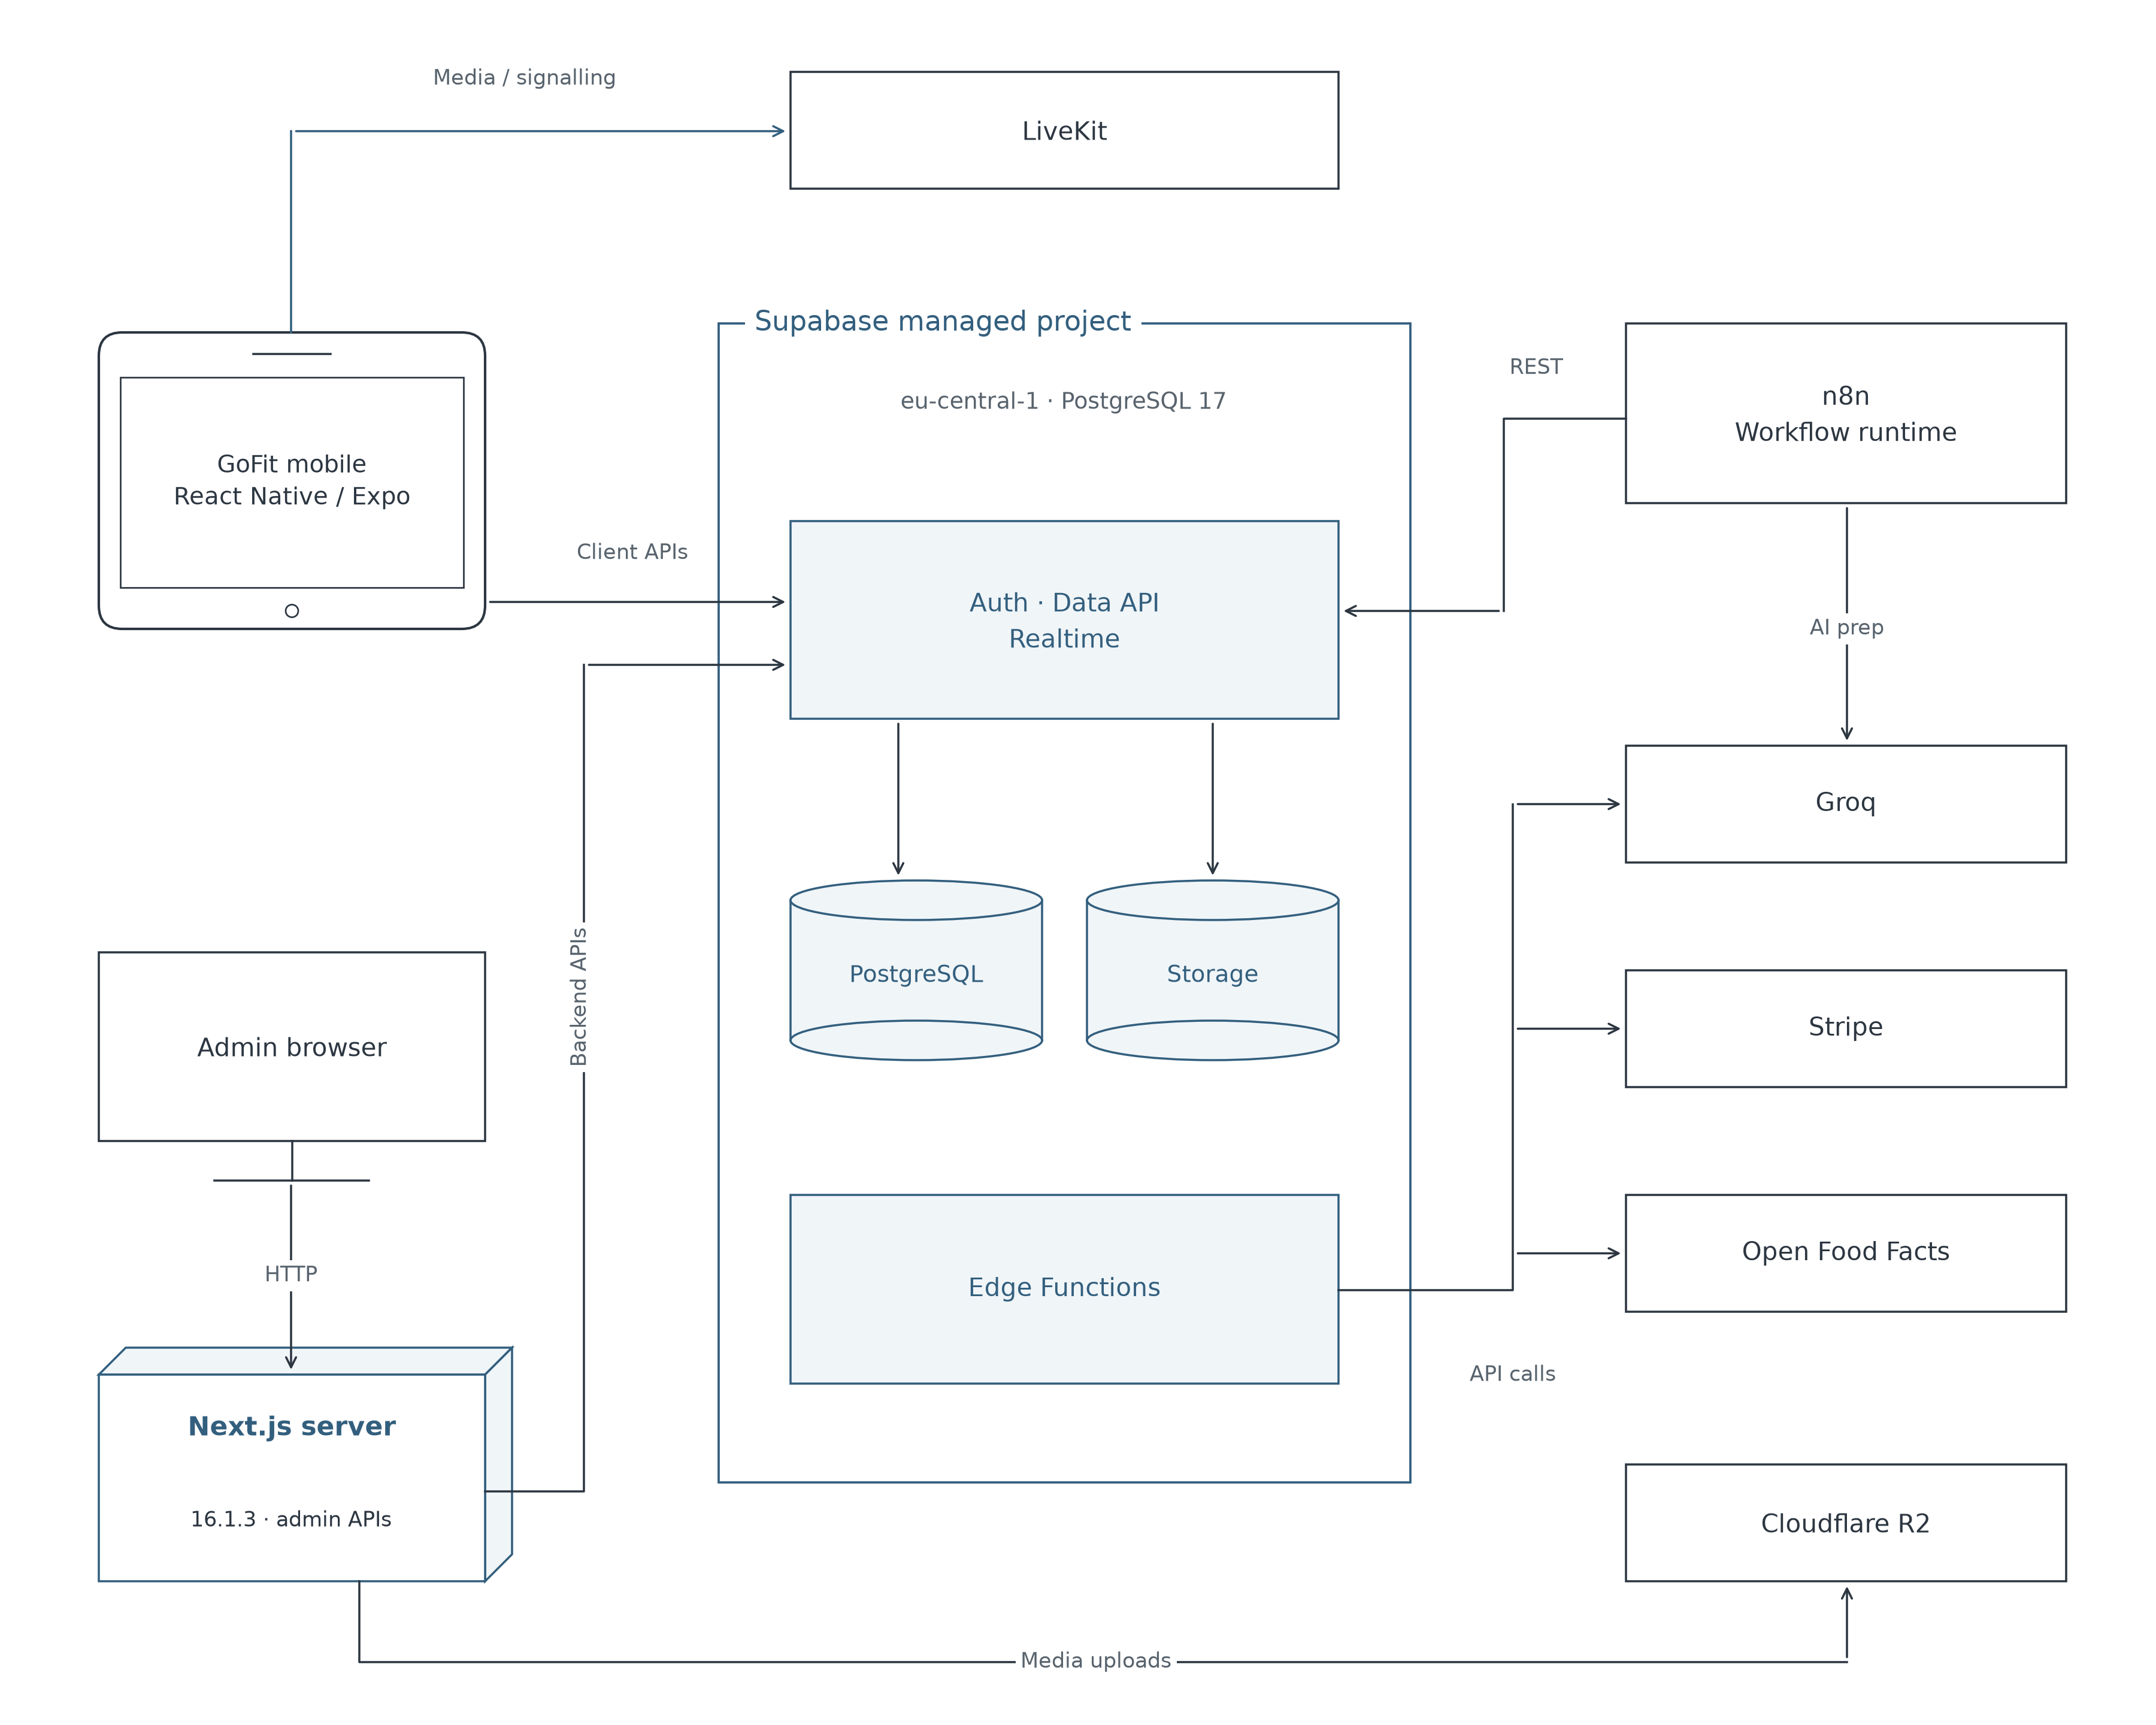
\includegraphics[width=0.95\linewidth]{figures/arch_physical.png}
\caption{GoFit execution environments and selected communication paths}
\label{fig:arch_physical}
\end{figure}

Figure~\ref{fig:arch_physical} presents execution environments and selected communication paths identified in the source. The mobile application targets Android and iOS using React Native 0.81.5 and Expo SDK 54. Platform-specific native modules remain relevant: the Android MediaPipe implementation does not establish equivalent iOS measurement support. Local persistence uses AsyncStorage and SecureStore in the inspected paths; no application-owned SQLite persistence layer is established by those paths. The administration interface has both a browser component and a Next.js 16.1.3 server runtime for rendering, API routes, access checks, and privileged adapters.

The inspected Supabase project was healthy in region eu-central-1 and reported PostgreSQL engine 17, build 17.6.1.054. Auth, Data API, Realtime, Storage, and Edge Function source form the selected managed-backend boundary. Application database requests use the configured Supabase clients and APIs; the diagram does not represent direct mobile database connections or provider-private gateway topology. The metadata does not establish multi-zone replication, a particular TLS version, or successful deployment and execution of every function.

Edge Function implementations call Groq for AI requests, Stripe for PaymentIntent creation, and Open Food Facts for barcode lookup. The video-token function signs a token locally using configured backend credentials and returns the LiveKit URL; the mobile SDK connects separately to LiveKit for signalling and media. The token function does not need a remote LiveKit token-minting request. The admin upload route sends media to Cloudflare R2, while mobile views use stored media URLs. The diagram selects the principal routes; mobile media retrieval, PaymentSheet internals, and the direct n8n-to-Groq call are summarized by node text and the detailed interaction/automation views.

The n8n runtime is a separate privileged caller using Supabase REST endpoints. AI Session Prep calls Groq directly, rather than invoking the coach-action AI Edge Function. Workflow exports and a Docker quick-start are available; the reviewed evidence does not establish the automation host, workflow activation, or successful scheduled runs. Similarly, a Next.js server is required by the code, but its production hosting provider is not confirmed here.

\subsection{Technologies and Selection Rationale}

The principal technology choices support the following implementation goals:

\noindent\textbullet\enspace Expo SDK 54 and React Native provide a shared TypeScript application structure and access to native device modules. Native dependencies require suitable builds, and code sharing does not establish feature parity across platforms.\par

\noindent\textbullet\enspace Supabase supplies managed authentication, database APIs, storage, and realtime capabilities. Database policies support authenticated access control; service-role callers operate with elevated privileges and require separate server-side checks. This choice reduces custom infrastructure without guaranteeing isolation under every application or policy error.\par

\noindent\textbullet\enspace Next.js App Router separates browser interactions from server-rendered pages, protected route handlers, and privileged backend/media adapters. The implemented request proxy and route checks support administrative access control.\par

\noindent\textbullet\enspace On-device pose and segmentation processing avoids a cloud inference request for the measurement captures in the inspected flow. Estimates still require quality checks and user review; local processing alone does not establish accuracy, latency, or complete privacy guarantees. The separate progress-photo feature can upload photos to managed storage.\par

\noindent\textbullet\enspace Groq is the configured provider for the inspected AI handlers and AI Session Prep workflow. Provider/model selection is an implementation choice; no response-time or token-throughput benchmark is established by these source files.\par

\subsection{Layered Architecture}

The implementation separates several responsibilities, with some direct calls across the suggested layers:

\noindent\textbullet\enspace Presentation: React Native screens, navigation, and reusable components render data and handle interaction. Screens also contain local state and, in selected paths such as measurement saving and checkout initiation, direct Supabase calls.\par

\noindent\textbullet\enspace Shared state: Zustand stores hold cross-screen data and coordinate selected service operations. Persistence is configured for specific stores and preferences; not every state change is durably cached.\par

\noindent\textbullet\enspace Services and adapters: TypeScript modules implement domain operations, transformations, API access, and device integration. Local native inference and device SDKs execute within the mobile boundary.\par

\noindent\textbullet\enspace Server execution: Next.js pages, proxy checks, API routes, Supabase Edge Functions, and n8n workflow code have distinct execution contexts. Server credentials and token/payment/AI handlers are not part of a shared browser or mobile state layer.\par

\subsection{Architecture Patterns: Local Persistence, Retry, and Realtime}

Offline support is scoped to implemented paths. Timer preferences are persisted locally. Workout completion for an already-created session can be queued in AsyncStorage when its remote update fails and connectivity is reported absent. The application's connectivity listener later invokes queue synchronization, retrying updates and removing successful entries. Session creation still requires the remote request, and the queue does not establish durable storage for every set interaction, execution while the application is terminated, or guaranteed absence of data loss. Other operations, including the measurement save path, do not use this workout queue.

Realtime subscriptions are implemented for selected data, including conversation messages and workout-session changes. Other screens use explicit refreshes or focus-triggered queries; nutrition logging and booking creation should not be described as universally subscription-driven. Source subscriptions establish the intended update mechanism, not instantaneous delivery on every device. The reviewed structure also does not establish a separate command/query infrastructure warranting a general CQRS implementation claim.

\subsection{Logical Architecture Diagram}

\begin{figure}[H]
\centering
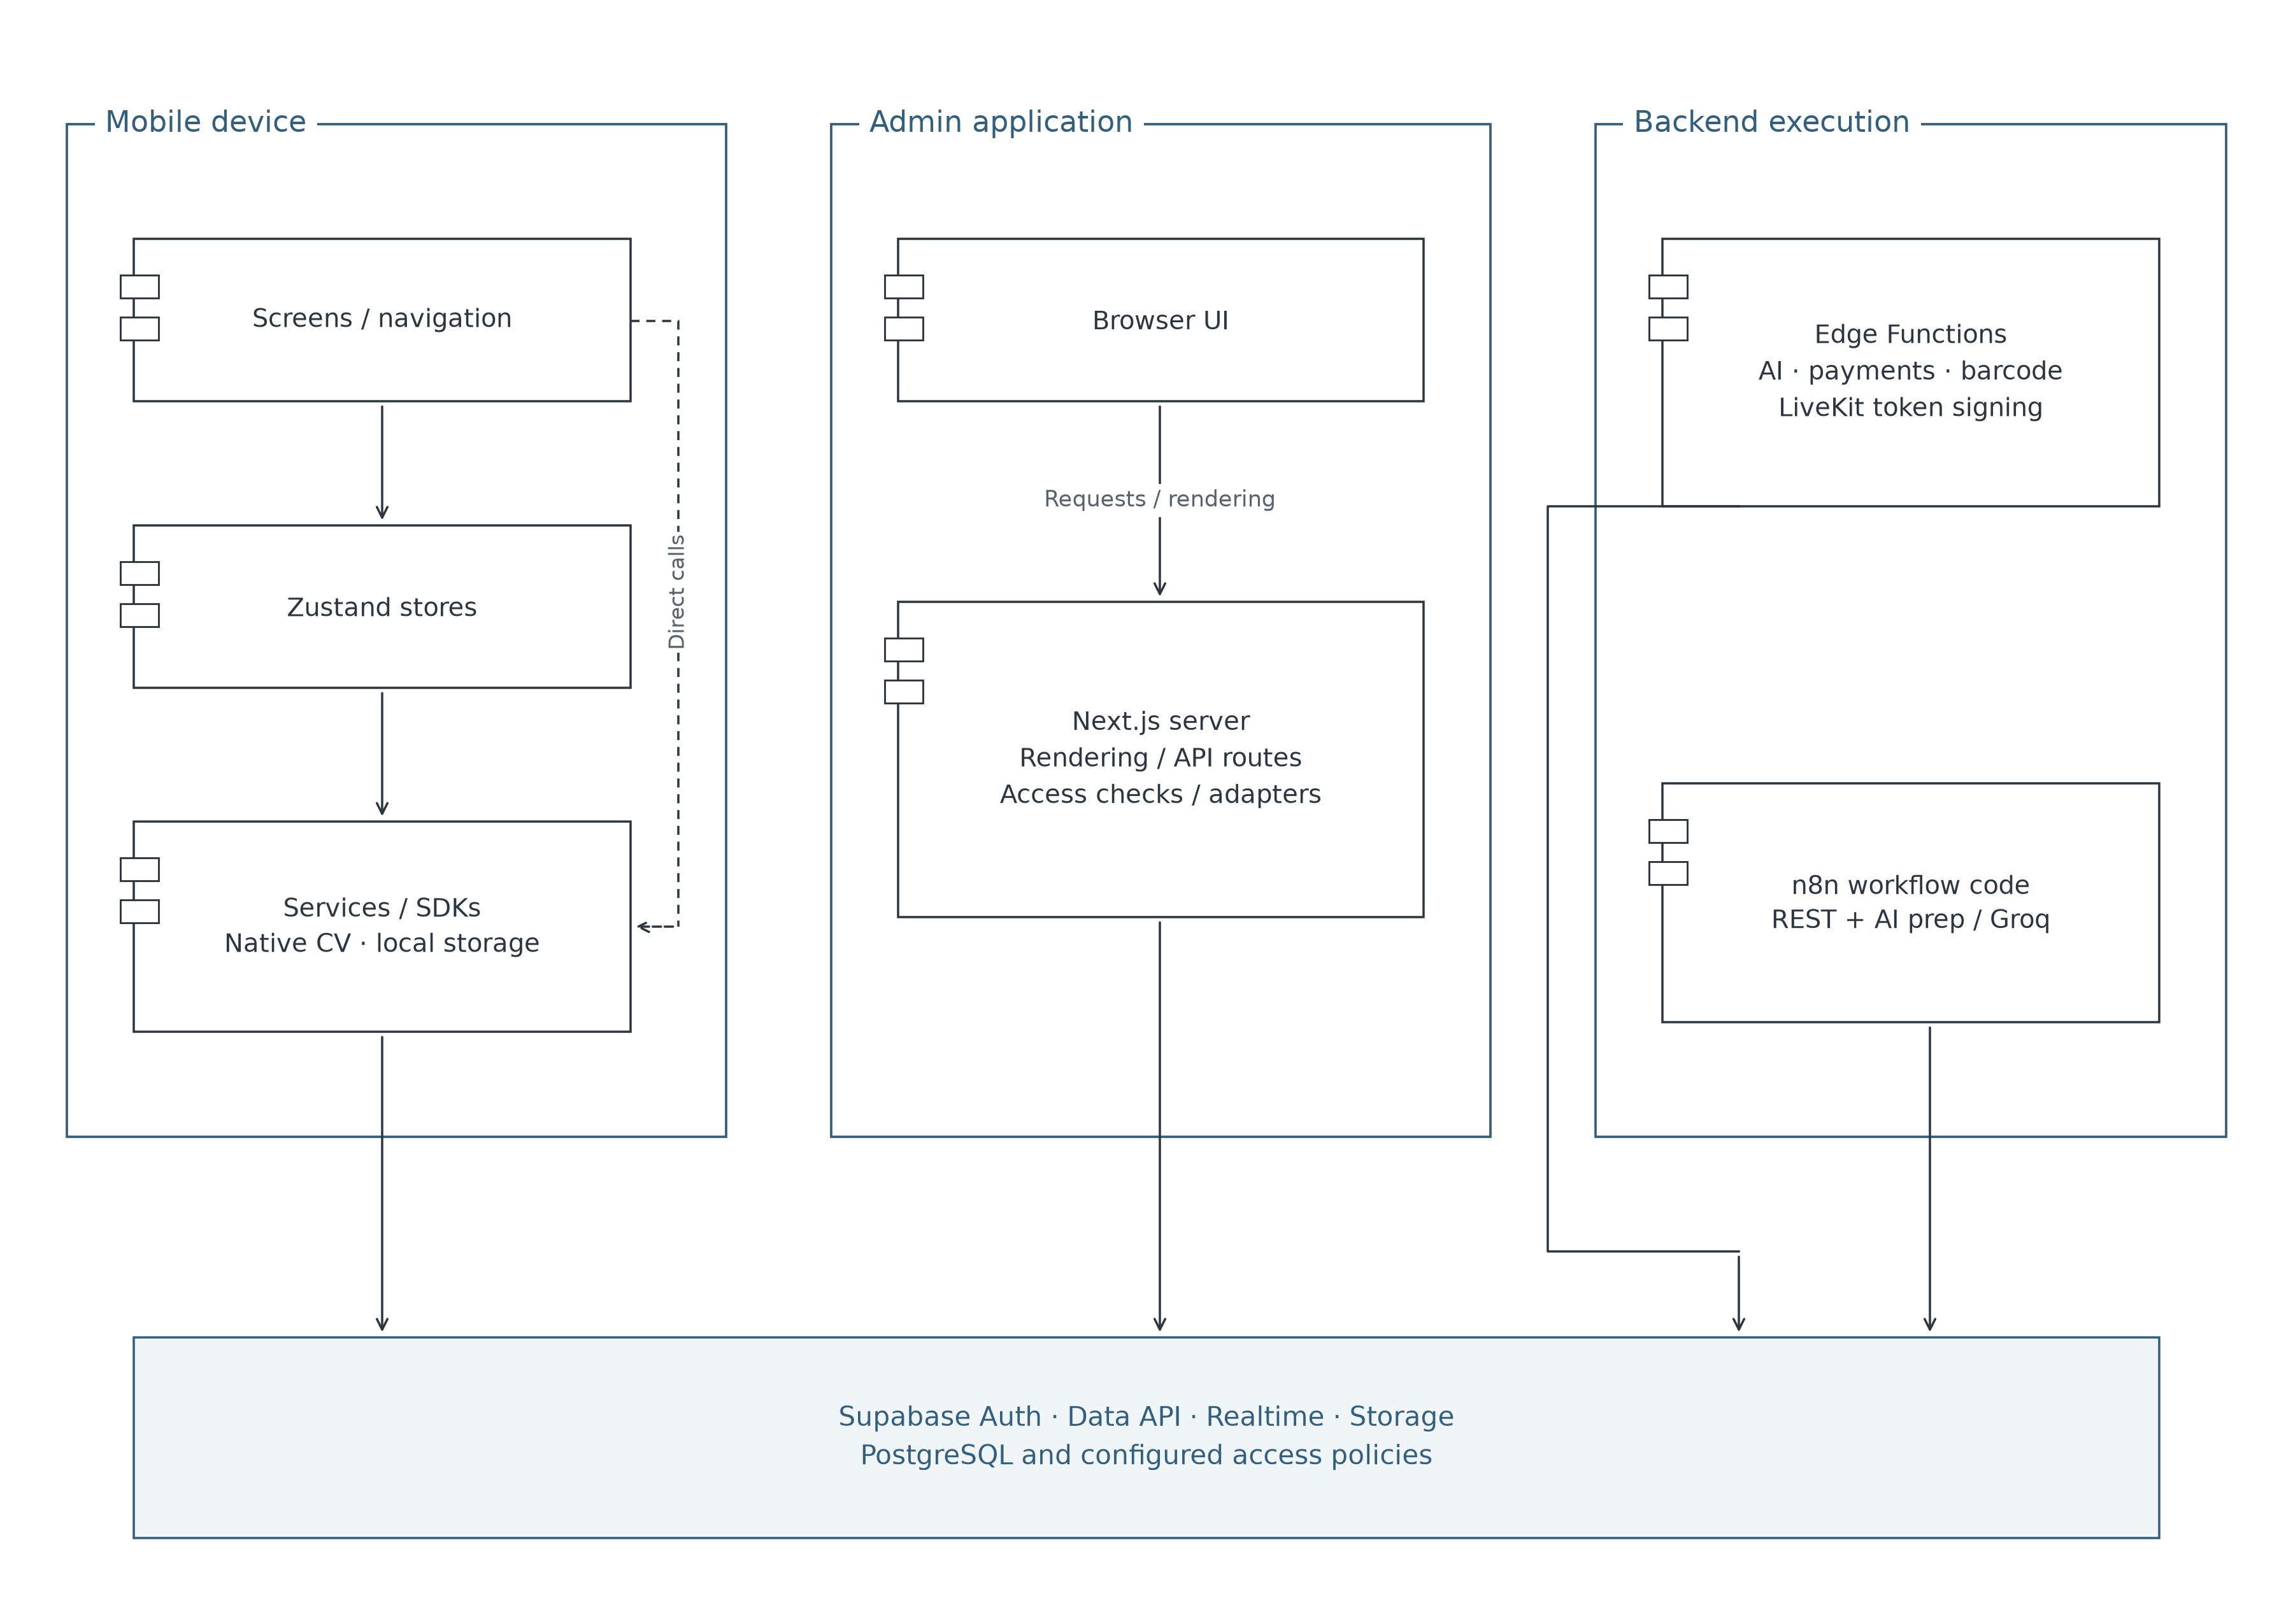
\includegraphics[width=0.95\linewidth]{figures/arch_logical.png}
\caption{GoFit logical responsibilities and execution boundaries}
\label{fig:arch_logical}
\end{figure}

Figure~\ref{fig:arch_logical} groups responsibilities by execution boundary rather than requiring every operation to traverse one shared stack. Mobile screens can call stores, services, or configured clients directly. Forms, filtering, and table state belong to browser presentation; declared UI-library dependencies do not establish a general server-cache tier. Native CV remains on the device, while privileged administration, payment intent creation, AI handlers, and token signing execute in their server contexts. Arrows represent selected dependencies; the view does not enumerate every domain module or external integration.

The mobile responsibilities summarized above are selected boundaries rather than mandatory call chains: screen code can access configured clients directly, stores coordinate some shared state, and native inference remains device-specific. The detailed workout, authentication, measurement and nutrition sequences provide the operation-level persistence boundaries.

\subsection{GoFit Administration Panel Architecture}

The administration panel provides a controlled back-office interface. It is designed separately from the mobile application because administrators need operational views, management tables, filters, analytics, settings, and privileged actions that should not be exposed in the client application. The panel uses protected routing and server-side Supabase access to keep administrative operations behind explicit authorization checks.


The retained administrative QA includes selected administrator, unauthenticated and non-admin access checks. These scoped results are summarized in Section~\ref{sec:qa-evidence}; they do not certify every route, policy or destructive operation.


\subsection{Admin BI Data Architecture}

The BI service modules read daily metric views, including \texttt{bi\_finance\_daily}, \texttt{bi\_user\_lifecycle\_daily}, \texttt{bi\_coach\_ops\_daily} and \texttt{bi\_client\_health\_daily}, then prepare dashboard data. Routes under \texttt{/api/bi} support exports, saved views, snapshots and digest-related operations. These are source-defined responsibilities; selected CSV, saved-view and population-label checks do not validate every aggregate or scheduled route.

The finance scope is primarily gross pack sales. Available history constrains lifecycle/cohort interpretation, and risk queues are operational indicators. The sandbox exclusion verified for the Transactions live total does not certify every BI finance aggregate; card payments, wallet ledger entries and coach payouts must remain distinct.

\subsection{Supabase Backend, Data Security, and Realtime Services}

The Supabase backend centralizes authentication, PostgreSQL data, storage, realtime communication and Edge Functions. Each client/coach data path should enforce its intended record access, while privileged administration and automation use trusted server-side contexts. Service-role keys must not be bundled into the mobile client.

A read-only check on 24 October 2026 found RLS enabled on all 40 public application tables. This is an observed setting, not proof that every policy, privileged function or API path enforces the intended ownership rules. The security advisor also reported publicly executable and authenticated-role-executable \texttt{SECURITY DEFINER} functions and disabled leaked-password protection; these require review of intended access and configuration rather than being treated as proof of an exploit or a clean security audit.


\begingroup
\footnotesize
\setlength{\tabcolsep}{3pt}
\renewcommand{\arraystretch}{1.20}
\setlength{\LTpre}{5pt}
\setlength{\LTpost}{10pt}
\begin{longtable}{|L{3.67cm}|L{5.29cm}|L{5.73cm}|}
\caption{Backend and security components}\label{tab:pdf-94-45} \\
\hline
\rowcolor{entetetab}
Component & Role & Security/validation concern \\ \hline
\endfirsthead
\hline
\rowcolor{entetetab}
Component & Role & Security/validation concern \\ \hline
\endhead
Supabase Auth & Manages identity, sessions, password reset, and protected access. & Check session handling, role mapping, and logout/session expiration behavior. \\ \hline
PostgreSQL database & Stores users, workouts, sessions, measurements, coaches, bookings, packs, messages, programs, and admin data. & Validate foreign keys, migrations, indexes, and data consistency. \\ \hline
RLS policies & Restrict row access according to user, coach, and administrator roles. & Test user-scoped, coach-scoped, and admin-scoped queries with different accounts. \\ \hline
Storage & Stores user-uploaded files such as coach documents, media, or progress-related assets when enabled. & Check bucket policies, private/public access, and file ownership. \\ \hline
Realtime/chat & Supports live communication and status updates. & Validate conversation membership, message visibility, and realtime channel permissions. \\ \hline
Edge Functions & Execute privileged operations such as push notification relay, video-token generation, and AI/backend workflows. & Keep secrets server-side and verify authorization inside each function. \\ \hline
n8n automations & Run scheduled or event-driven workflows such as AI session preparation and admin operations digest. & Use service-role access only in controlled environments and log workflow results. \\ \hline
\end{longtable}
\endgroup

\subsection{Messaging, Video and Storage Security Boundaries}

The inspected chat service inserts the supplied message text directly into the message record and uses realtime subscriptions for updates. It also copies a message preview into notification payloads. No client-side encryption/decryption or participant key-management step was identified in this send path. Protected transport, managed storage and RLS are distinct controls; they do not establish end-to-end encrypted messaging. FR-06's encrypted-messaging wording remains a target requiring a defined threat model and implementation evidence.

The deployed video-token function (version 8) has gateway JWT verification enabled, but its handler accepts room and participant values from the request without binding them to an authenticated booking participant or checking booking status/time. The mobile service also enables a testing bypass of its join-window check. A signed room token and a client-side button therefore do not establish per-booking authorization. These are source/configuration findings; no unauthorized room join was attempted. Two-party media, permission, reconnect and release behavior remain unverified.

Session persistence uses the native SecureStore adapter, while its web fallback uses AsyncStorage; the workout-completion queue separately uses AsyncStorage. These mechanisms must not be grouped into a claim that all local data is encrypted or has equivalent security on every platform. Release-build storage behavior and the complete token lifecycle require their own checks.

The source references, deployed video-source comparison, read-only RLS result and advisor notices are retained in \path{qa/2026-10-24-step-3-claims/README.md}. This claims review does not change backend policies, the token handler or mobile code, and it does not certify the remaining security boundaries.


\subsection{Development Assistance and Review Procedure}

AI assistants, including Codex, supported repository inspection, implementation proposals, debugging, diagram drafts and report revision. Connected tools provided file, browser and selected backend context. These tools supplied material for review rather than proof that a feature was implemented, deployed or tested.

The review procedure compared generated claims with source files, examined changes and retained the relevant execution artifacts when checks were performed. Missing execution evidence remains explicit in the QA matrix. Generated documentation and mock-based tests cannot establish native behavior, provider outcomes or historical sprint completion.

The present report is maintained in LaTeX. Earlier document-generation scripts are part of the drafting history; their existence does not verify the current report's content or the application. Responsibility for accepting the implementation and academic claims remains with the author.

\subsection{n8n Automation Layer}

Five n8n exports in \path{../docs/automation/n8n/workflows} define scheduled briefing, reminder and digest operations using backend REST calls. They require a separate privileged runtime. The exports establish intended queries and writes, without establishing active hosting or successful scheduled execution.


The accompanying Docker quick-start documents a self-hosted runtime and environment-variable configuration. The service-role credential belongs in that server boundary; the Groq credential is needed by AI Session Prep. Configuration instructions do not establish that secrets were securely provisioned or that a container is running.


Each exported workflow uses a schedule trigger followed by a Code node. The exported canvases also include sticky-note cards that document the schedule window, query logic, duplicate guard, notification creation, and run summary. These exports establish the executable structure; evidence of successful scheduled runs and persisted outputs must be assessed separately.



\begingroup
\scriptsize
\setlength{\tabcolsep}{3pt}
\renewcommand{\arraystretch}{1.20}
\setlength{\LTpre}{5pt}
\setlength{\LTpost}{10pt}
\begin{longtable}{|L{2.20cm}|L{1.40cm}|L{3.90cm}|L{4.20cm}|L{3.90cm}|}
\caption{Configured n8n workflow logic in the supplied exports}\label{tab:pdf-99-49} \\
\hline
Workflow & Configured trigger & Data read & Defined actions & Source guard/control \\ \hline
AI Session Prep v1 & Every 60 minutes & Confirmed bookings in the next 24 hours, coach profile, client profile, recent completed sessions, private coach notes, and recent check-ins. & Calls Groq from n8n, inserts an \texttt{ai\_session\_notes} row, and creates a coach notification with \texttt{data.kind = ai\_session\_ready}. & Skips unexpired existing notes for the same coach/client pair and repairs missing coach notification when needed. \\ \hline
Booking Reminders v1 & Every 15 minutes & Confirmed bookings starting within the next 60 minutes plus coach user mapping. & Creates one client notification and one coach notification with \texttt{data.kind = booking\_starting\_soon}. & Skips duplicate reminders for the same booking, recipient role, and 60-minute window. \\ \hline
Check-in Reminders v1 & Every 4 hours & Enabled \texttt{check\_in\_schedules}, current UTC date/time and \texttt{check\_in\_responses} for the day. & Creates a client notification with \texttt{data.kind = check\_in\_due}. & Skips schedules not due, clients who already responded, and existing reminders for the same schedule/date. \\ \hline
Coach Daily Digest v1 & Daily & Coach profiles, check-in schedules and responses, upcoming confirmed bookings, active packs, booking history, and BI client-health daily rows. & Creates a coach notification summarizing missed check-ins, low wellness signals, upcoming sessions, and inactive clients. & Skips coaches with no useful signal and skips duplicate digest notifications for the same coach and UTC date. \\ \hline
Admin Ops Digest v1 & Daily & Admin user profiles, new users, pending coaches, booking outcomes, and pack purchases from the last 24 hours. & Creates an \texttt{admin\_notifications} row per administrator with operational counts and a deterministic digest link. & Skips duplicate admin digests for the same admin, title, and date link; \texttt{automation\_failures\_count} remains 0 in v1 because failures are not yet persisted. \\ \hline
\end{longtable}
\endgroup

The exported workflows create in-app notification records rather than direct push deliveries. UTC comparisons and existing-row checks implement the documented scheduling and duplicate guards, without establishing concurrency-safe exactly-once execution. Runtime authorization, client visibility of coach briefings and secret handling require their own deployment checks. No fresh scheduled run, replay-under-concurrency result or provider delivery receipt is retained.

\begin{figure}[H]
\centering
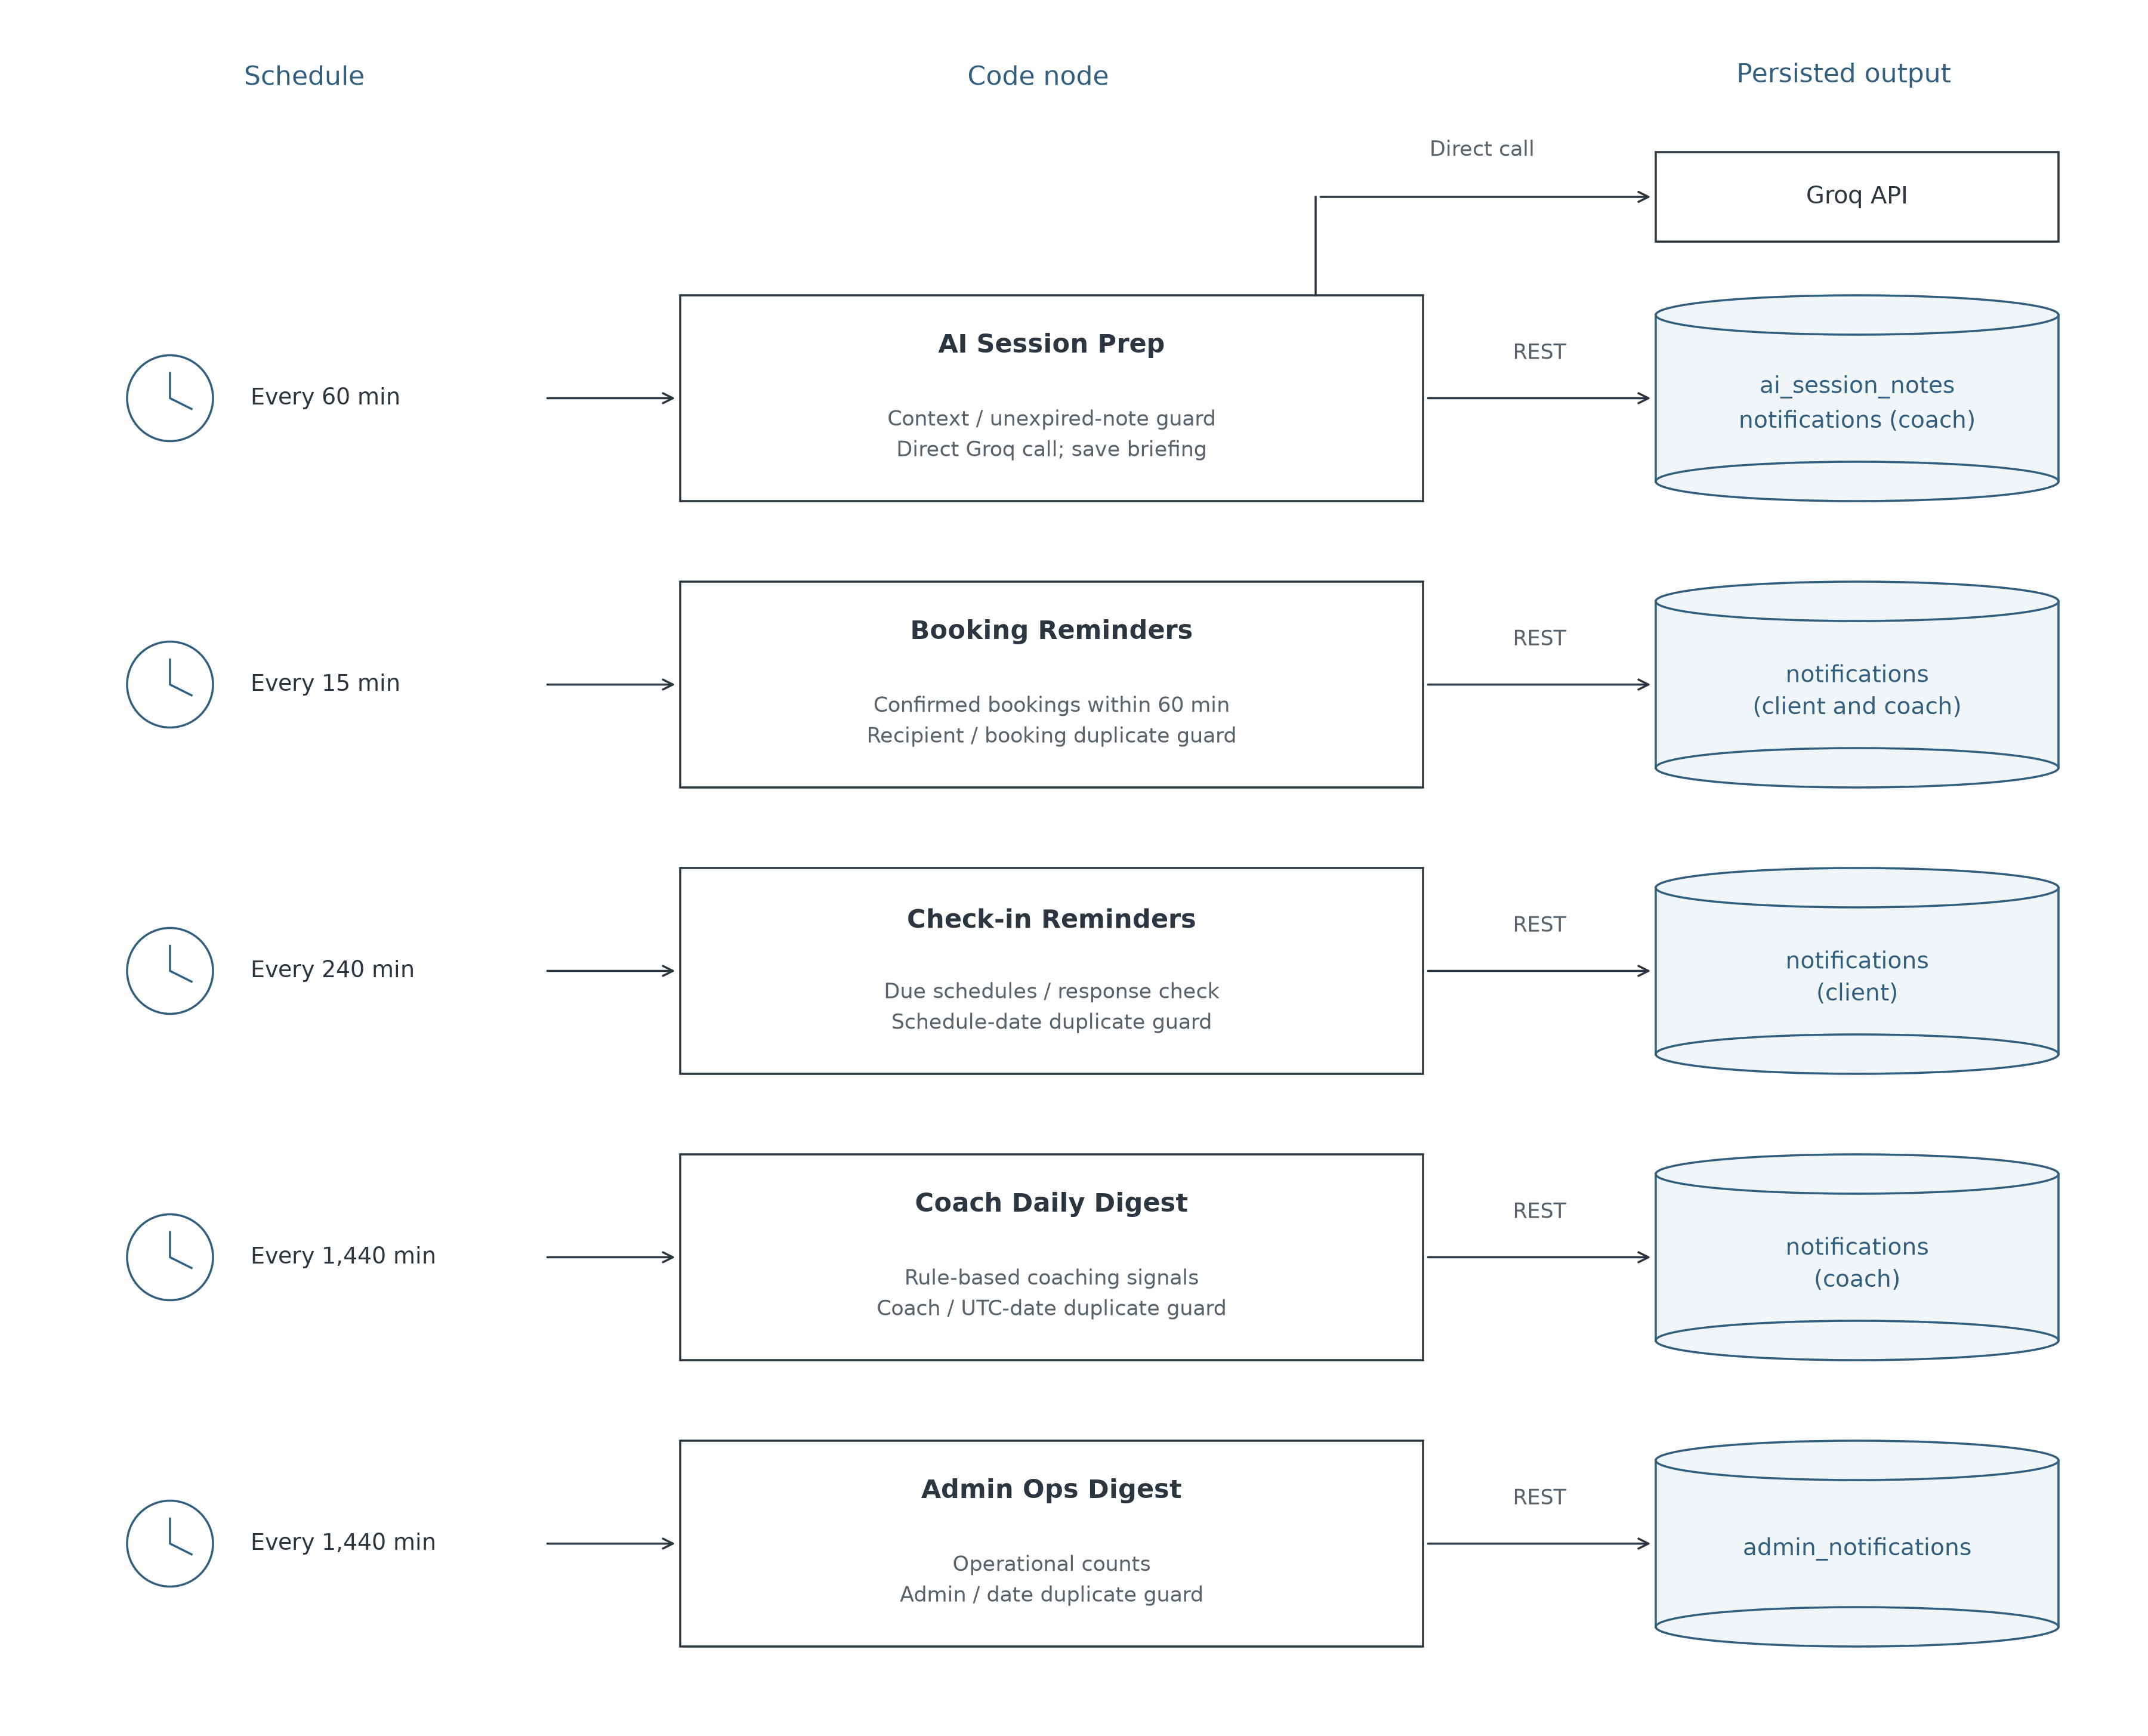
\includegraphics[width=0.92\linewidth]{figures/n8n_automation.png}
\caption{Five exported n8n workflows, configured intervals, and persisted outputs}
\label{fig:n8n_automation}
\end{figure}

Figure~\ref{fig:n8n_automation} follows the supplied workflow exports. Each executable path consists of a Schedule Trigger and one Code node; sticky notes document internal stages rather than adding executable template nodes. Intervals are 60 minutes for AI Session Prep, 15 for Booking Reminders, 240 for Check-in Reminders, and 1,440 for each digest. These intervals do not establish a fixed 08:00 UTC schedule or a weekly trigger. Code performs backend REST queries and writes, applying workflow-specific duplicate checks. AI Session Prep calls Groq directly and persists a briefing; Coach Daily Digest aggregates rule-based signals. Outputs are in-app notification rows or admin-notification rows, with no direct Expo push or Resend email delivery in these exports. Existing-row checks reduce duplicate creation but are not proof of concurrency-safe exactly-once execution. The exports do not specify an active deployment, and successful run evidence remains separate from implementation artifacts.


No successful scheduled-run screenshot is added for automation: the retained artifact is the workflow design in Figure~\ref{fig:n8n_automation}, while execution and delivery evidence remain pending. Similarly, the architecture/deployment views describe their stated targets and metadata rather than serving as screenshots of a published release.

\subsection{Device Feedback and Validation Scope}

The session screen contains haptic calls for set completion and selected actions; timer configuration also exposes feedback preferences. Such calls establish an intended device interaction, not observed vibration timing or locked-device delivery. The controlled timer scenario remains unverified in Section~\ref{sec:qa-evidence}. Package families and platform boundaries are summarized once in Table~\ref{tab:pdf-88-43}; a dependency inventory does not demonstrate complete feature coverage.

\section{Deployment}

\subsection{Deployment Diagram}

\begin{figure}[H]
\centering
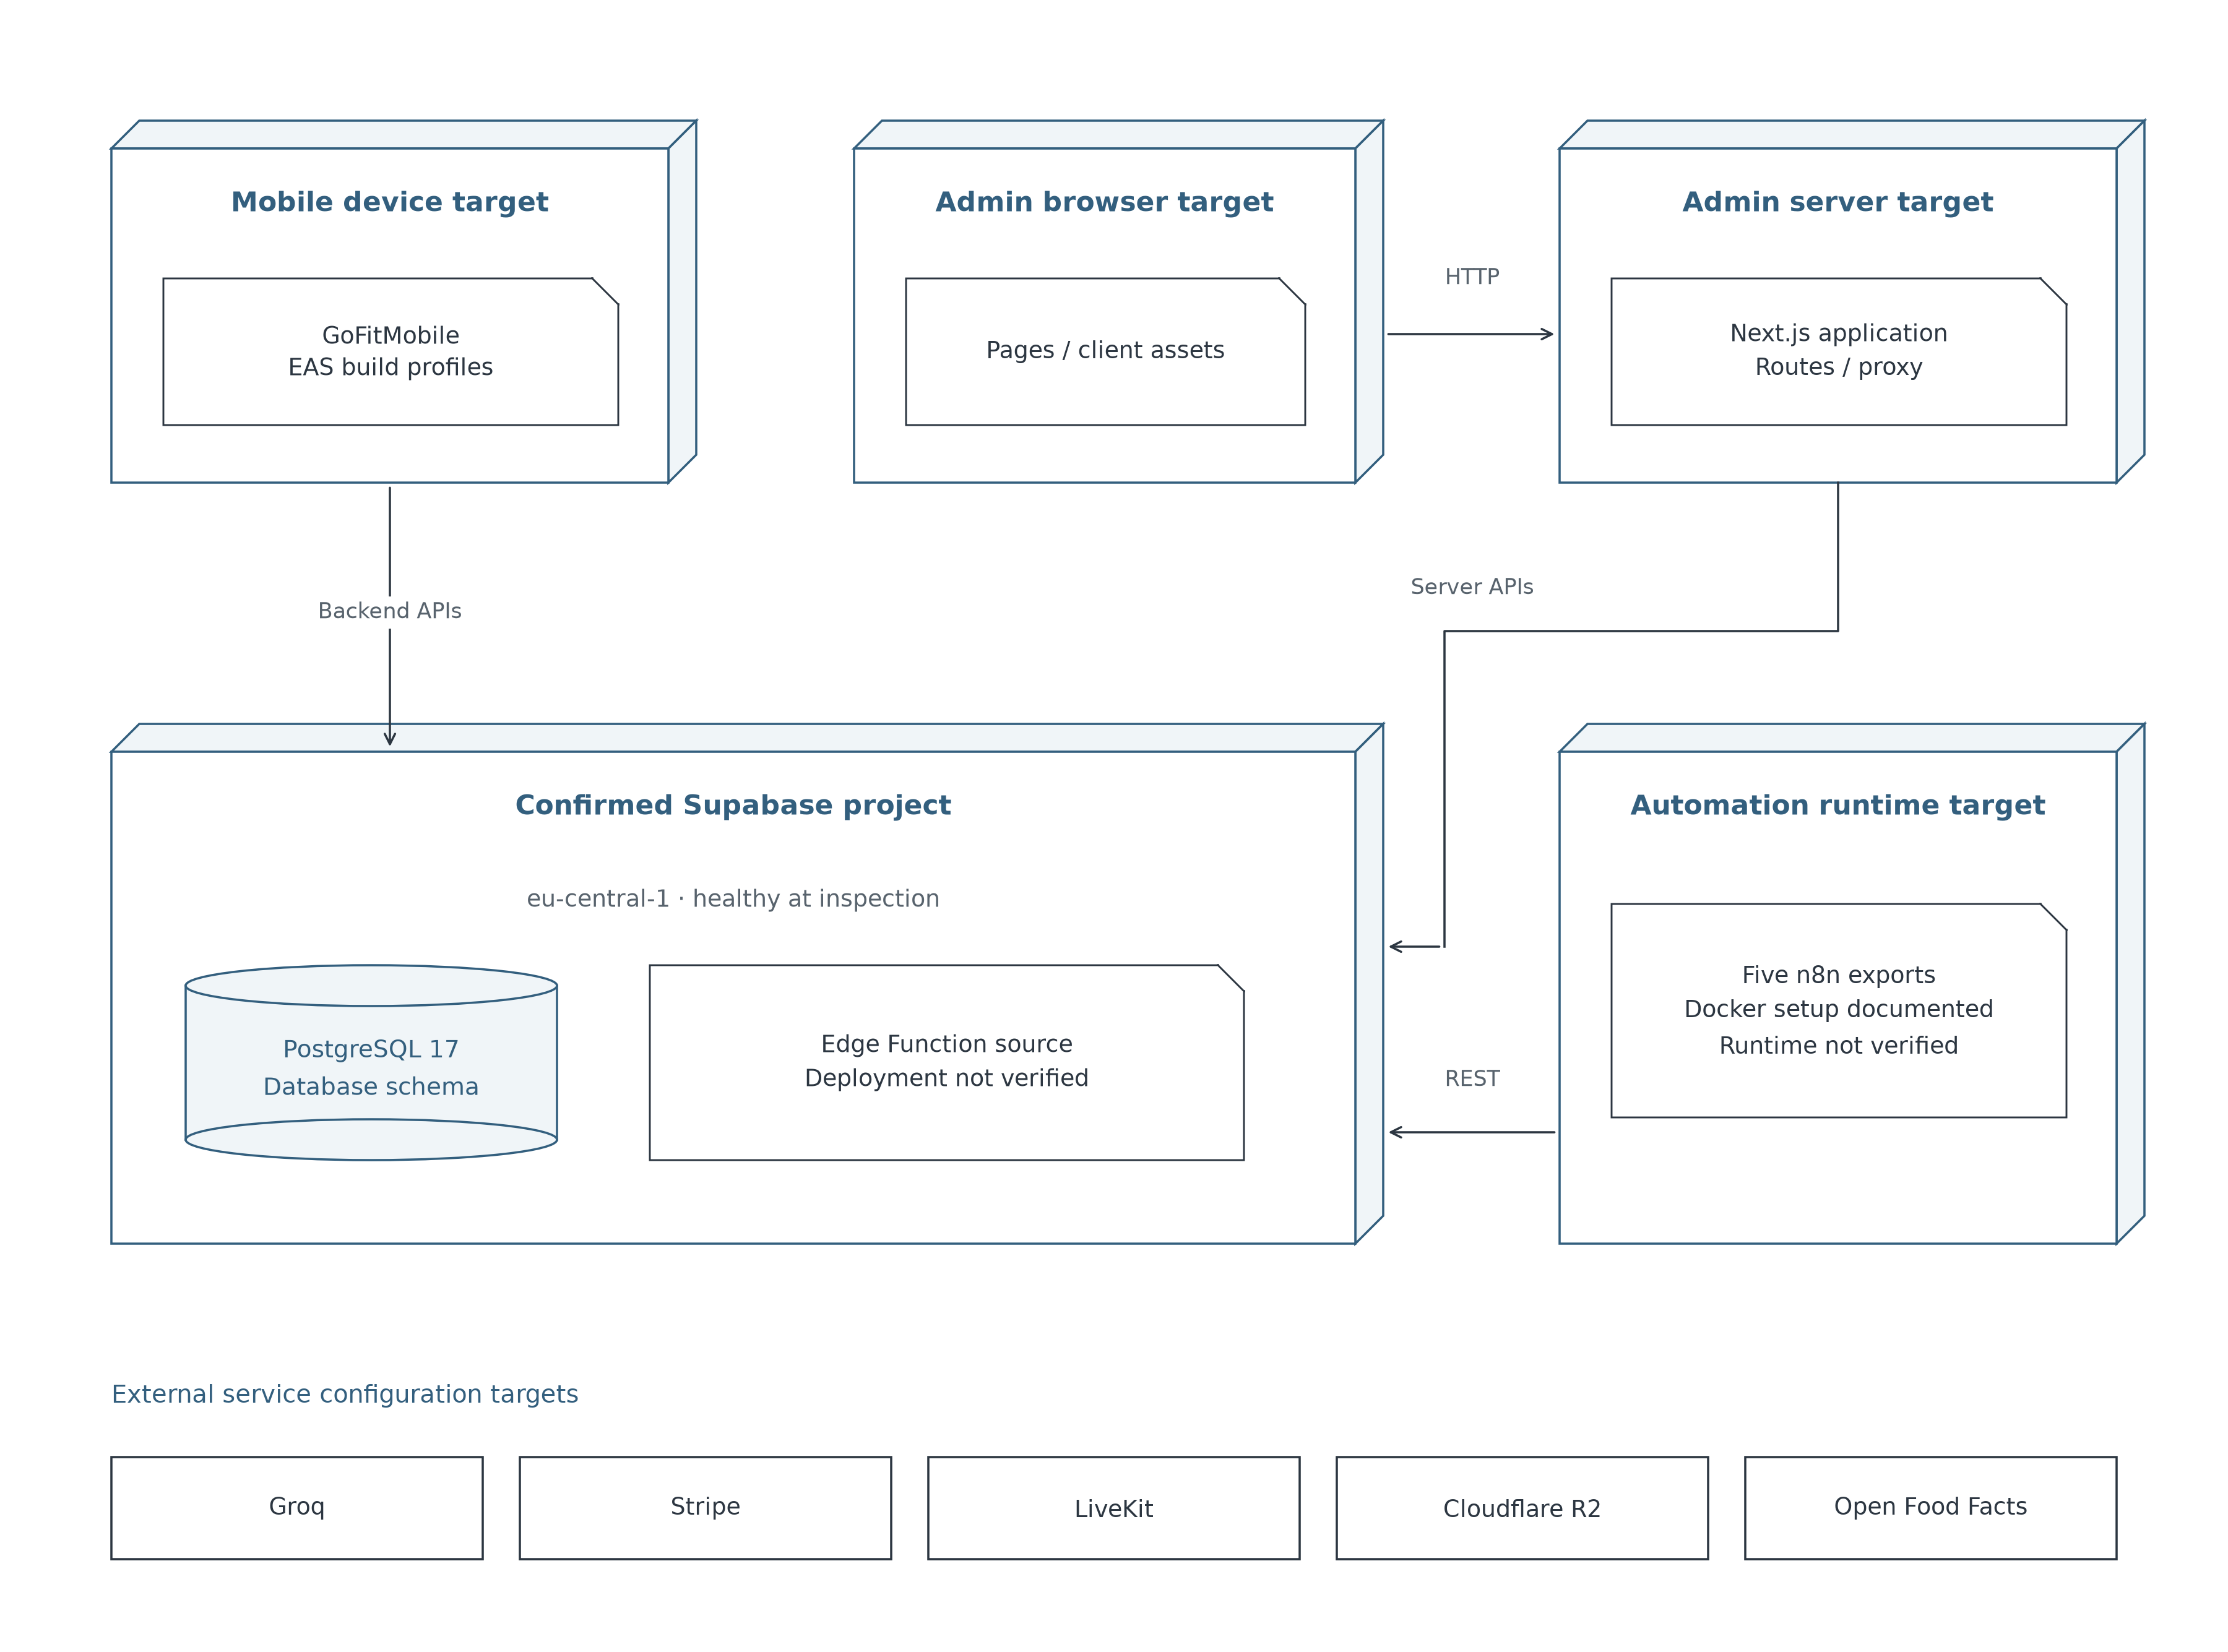
\includegraphics[width=0.95\linewidth]{figures/deployment_diagram.png}
\caption{Deployment targets and the confirmed managed-backend environment}
\label{fig:deployment_diagram}
\end{figure}

Figure~\ref{fig:deployment_diagram} distinguishes source/configuration targets from the inspected backend project. Mobile, browser, Next.js server, and automation artifacts require different runtimes. The Supabase project's health, region, and database version were inspected; the diagram does not assert verified mobile distribution, admin hosting, every Edge Function deployment, or active automation. External-service configuration targets are listed with their callers rather than represented as a remote token-minting dependency.

\subsection{Build Configuration and Deployment Evidence}

The available repository artifacts support the following deployment description:

\noindent\textbullet\enspace Mobile build configuration: \texttt{GoFitMobile/eas.json} defines development, preview, and production profiles. Development enables a development client and internal distribution; preview also selects internal distribution, while production enables version auto-increment. These profiles do not by themselves prove separate environment URLs, successful builds, signing setup, or store publication.\par

\noindent\textbullet\enspace Admin runtime: the Next.js package defines development, build, start, lint, and test scripts. Its route handlers and server-side clients require a server-capable deployment. The reviewed configuration does not substantiate a Vercel project link, pull-request previews, merge-triggered production releases, or specific remote checks.\par

\noindent\textbullet\enspace Managed backend: database scripts and Edge Function implementations are versioned artifacts. The 21 October metadata snapshot in \path{deployment-verification.md} recorded 60 migration entries and 40 public tables; later payment migrations have their separate dated evidence. This earlier count is not a current complete migration inventory, and filename matching does not establish that every local SQL script was applied or that matching names imply identical contents. No deployment run or local Deno test is inferred merely from source files or CLI instructions.\par

\noindent\textbullet\enspace Automation: five versioned JSON exports and a documented local Docker quick-start provide an import/deployment starting point. Runtime secrets, persistence, activation, and scheduled-execution evidence require confirmation for the selected host. The exports and instructions are not evidence that a production container is running.\par

\noindent\textbullet\enspace External integrations: Groq, Stripe, LiveKit, Cloudflare R2, and Open Food Facts appear in implementation or configuration paths. Operational status, payment settlement, media delivery, video interoperability, and response-time claims require their own execution evidence.\par

\subsection{Implementation Evidence Matrix}
\label{sec:implementation-evidence}

Table~\ref{tab:implementation-evidence} maps the eight functional requirements defined in Sprint 0 to the inspected implementation and the retained October 2026 evidence. Implementation extent and verification are separate: an identified screen or service is evidence of a code path, while a successful scenario requires its own execution record. A partial target denotes a known difference between the stated requirement and the inspected path. No row certifies the complete functional domain as implemented and validated.

The detailed index in \path{qa/2026-10-24-step-2-evidence-matrix/matrix.md}, supported by its machine-readable \path{qa/2026-10-24-step-2-evidence-matrix/matrix.json}, records source files, line anchors, file hashes, QA case identifiers and limitations. M01--M20 are local audit references rather than new requirement or backlog identifiers. C, H, A, P and S refer to the evidence package defined in the following QA subsection. Source presence alone does not establish that a local SQL script or integration has been deployed; payment deployment and provider results are supported only by their separate retained follow-ups.

\begingroup
\footnotesize
\setlength{\tabcolsep}{3pt}
\renewcommand{\arraystretch}{1.20}
\setlength{\LTpre}{5pt}
\setlength{\LTpost}{10pt}
\begin{longtable}{|L{1.15cm}|L{3.35cm}|L{2.05cm}|L{3.95cm}|L{4.10cm}|}
\caption{Functional requirements, implementation extent and retained evidence}\label{tab:implementation-evidence} \\
\hline
\rowcolor{entetetab}
Requirement & Inspected implementation scope & Implementation extent & Supporting verification & Limitations \\ \hline
\endfirsthead
\hline
\rowcolor{entetetab}
Requirement & Inspected implementation scope & Implementation extent & Supporting verification & Limitations \\ \hline
\endhead
FR-01 & Authentication\slash{}recovery services, six-screen onboarding, profile and nutrition-preference editors & Partial target & M01--M02; existing client\slash{}coach session relaunch and approved-coach routing; profile views; editor\slash{}model regressions & Full equipment\slash{}fitness-level questionnaire absent from the inspected onboarding path. Fresh registration\slash{}recovery and recent editor\slash{}contrast native retests remain pending. \\ \hline
FR-02 & Exercise catalog\slash{}search\slash{}filter paths; custom workout create\slash{}edit\slash{}delete and configured prescriptions & Partial target & M03--M04; C: catalog\slash{}detail and disposable workout CRUD; mocked summary regressions & All filters\slash{}media and boundary validation incomplete. Dedicated reorder and target-load controls not located in the inspected builder. Summary correction awaits Android. \\ \hline
FR-03 & Weights\slash{}completion snapshots, configured reps, rest-timer code and AsyncStorage completion-update retry & Partial target & M05--M06; session\slash{}queue source inspected; C: SESSION-01--07 blocked & Independent performed-repetition\slash{}RPE input absent from the inspected path. No controlled locked-device timer or offline reconciliation; queue requires an existing remote session. \\ \hline
FR-04 & Progress\slash{}record views, weight editing, photo services and body-capture\slash{}estimation\slash{}review code & Paths identified; AI integration foundation & M07--M08; C: existing charts, records, photo detail and measurement history; camera-denial observation & Fresh photo\slash{}biometric persistence, inference\slash{}edit-save and independent accuracy comparisons incomplete. Platform-limited native integration does not establish iOS support. \\ \hline
FR-05 & Nutrition search\slash{}logs\slash{}totals\slash{}goals, saved meals, barcode lookup and name-based exclusions & Paths identified & M09; C: food search and disposable log add\slash{}remove; narrower saved-meal\slash{}goal\slash{}permission observations & Actual barcode\slash{}provider lookup, reuse\slash{}edit and controlled exclusion cases unverified. Name matching does not establish comprehensive allergen exclusion. \\ \hline
FR-06 & Coach discovery\slash{}reviews, pack checkout, availability\slash{}reservation and communication integration paths & Mixed: scoped payments verified; other paths identified & M10--M13; P: Android EUR129\slash{}12-credit pack; S: EUR60 session API\slash{}admin capture, replay and conflict checks; list\slash{}entry observations & Native standalone booking and two-party communication pending. Pack-credit booking branch, encrypted-messaging guarantees, payment recovery\slash{}refunds\slash{}payouts and production behavior not certified. \\ \hline
FR-07 & Coach roster\slash{}progress\slash{}notes\slash{}check-ins, workout\slash{}meal program model\slash{}services and client-context briefing & Partial target & M14--M16; H: roster\slash{}detail\slash{}private-note CRUD and scoped query\slash{}streak corrections; lists\slash{}validation\slash{}empty states & Populated scheduling\slash{}program assignment and fresh AI generation unverified. Briefing concerns pre-session client context rather than completed-consultation synthesis. Template service presence does not prove complete reachable UI. \\ \hline
FR-08 & Role-protected admin routes, catalog CRUD, coach-review API, transactions, audit and BI paths & Paths identified; scoped operations verified & M17--M18; A: selected role checks\slash{}disposable CRUD; audit fixes; payment references; profile-count reconciliation; CSV\slash{}saved views & Actual approval\slash{}rejection\slash{}document verification, destructive account operations, every BI calculation and larger account listings remain unverified or partial. Audit insertion is not certified atomic. \\ \hline
\end{longtable}
\endgroup

The matrix also indexes adaptive workout recommendations (M19) and operational workflows/notification delivery (M20) as supplementary capabilities discussed in the report, without inventing additional numbered requirements. Their source artifacts exist, but reachable recommendation generation and fresh scheduled delivery remain unverified. The matrix records evidence boundaries. AI/security claims are qualified in the retained claims review, and the sprint-artifact cross-reference identifies the subsequent reconciliation. All later corrections and checks are dated as October follow-up work, rather than attributed retrospectively to the internship period.

\subsection{Automated Checks and Evidence-Based QA Status}
\label{sec:qa-evidence}

The following matrix distinguishes implemented workflows from verified outcomes and outstanding checks. Its evidence comes from the follow-up audit and corrections conducted on 22--24 October 2026, after the 26 January--26 July 2026 internship period. These later results describe the inspected development version; they do not establish that the same implementation or validation outcomes existed at the end of the internship. The sprint-level matrices have been reconciled with this retained evidence; their original task identifiers do not turn later observations into verified sprint-period results.

The retained device observations concern one Samsung SM-S928B running Android 17/API 37 with separate GoFit QA development packages. Administrative checks used a local Next.js development server and the configured Supabase backend. The latest recorded automated runs passed 146 mobile tests across 25 suites and 34 administrative tests. These tests cover their specified cases, often with mocked dependencies; they do not substitute for native integration or provider execution. The administrative TypeScript check passed, whereas the project-wide mobile check still reported 12 pre-existing diagnostics outside the recent corrections.

The current role-scoped ledgers record 30 passes, 23 partial cases and 24 blocked cases for the client; 22 passes, 11 partial cases and 12 blocked cases for the coach; and 35 passes, six partial cases and six blocked cases for administration. These populations overlap and must not be added into a count of unique requirements. Corrected source defects can remain partial until device retesting is completed. In Table~\ref{tab:pdf-113-56}, a scoped pass applies only to the stated routes and observations; partial denotes verified components within an incomplete scenario; not verified denotes an execution result for which retained evidence is insufficient.


\begingroup
\scriptsize
\setlength{\tabcolsep}{2pt}
\renewcommand{\arraystretch}{1.20}
\setlength{\LTpre}{5pt}
\setlength{\LTpost}{10pt}
\begin{longtable}{|L{1.20cm}|L{1.50cm}|L{1.60cm}|L{1.60cm}|L{1.80cm}|L{1.80cm}|L{1.65cm}|L{1.35cm}|L{2.00cm}|}
\caption{QA scenarios and evidence status: October 2026 follow-up}\label{tab:pdf-113-56} \\
\hline
\rowcolor{entetetab}
Test ID & Feature Area & Validation Scenario & Preconditions & Execution Steps & Expected Result & Observed Outcome & Status & Retained Evidence \\ \hline
\endfirsthead
\hline
\rowcolor{entetetab}
Test ID & Feature Area & Validation Scenario & Preconditions & Execution Steps & Expected Result & Observed Outcome & Status & Retained Evidence \\ \hline
\endhead
QA-01 & Authentication and onboarding & Registration, profile setup and session persistence & Existing client\slash{}coach accounts; disposable account needed for registration & Relaunch existing QA apps; fresh registration not executed & Existing session retained; new-account setup verified separately & Existing sessions resumed; approved-coach routing retested. Fresh onboarding, token-storage details and refresh not established & Partial & C: AUTH-01\slash{}02\slash{}04; H: AUTH-03\slash{}04\slash{}05 \\ \hline
QA-02 & Workout timer & Locked-device rest timer, sound and vibration & Controlled workout fixture and unlocked\slash{}locked-device observations & Planned: log sets; start 90-second timer; lock device; record expiry behavior & Timer, sound and vibration follow the specified behavior & User reported operation; no retained controlled reproduction of the complete scenario & Not verified & C: SESSION-03\slash{}04; no controlled timer trace retained \\ \hline
QA-03 & Offline synchronization & Offline logging and reconnection & Disposable workout and captured queue\slash{}network state & Planned: log offline; finish; reconnect; compare queue and saved rows & Intended entries reconciled without loss or duplication & No retained end-to-end reconciliation, queue dump or timestamp comparison & Not verified & C: SESSION-07; no offline trace retained \\ \hline
QA-04 & Body measurements & Capture, inference and draft review & Required captures and calibration; independent references for accuracy & Planned: capture inputs; run analysis; retain output and review state & Draft generated; accuracy evaluated separately against references & History\slash{}permission observations do not prove new inference or measurement accuracy; no supported numerical outcome & Not verified & C: \seqsplit{MEASUREMENT}-01--05; no retained inference\slash{}accuracy result \\ \hline
QA-05 & AI recommendations & Reachable generation and output review & Eligible account and configured backend & Reach recommendation entry; retain response and timing if executed & Structured workout with catalog-backed exercises & Tested account has session history and cannot reach the inspected recommendation entry; generation\slash{}timing unverified & Not verified & C: AI-01--03; no generation response retained \\ \hline
QA-06 & Sandbox payments and booking & Pack purchase and standalone paid session & Stripe sandbox; approved coach; configured availability & Android 12-credit pack purchase; separate API session capture, replay and conflict checks & Verified payment linked to credits or booking; occupied slot refused & EUR129 pack\slash{}12 credits saved on Android; EUR60 session saved via API\slash{}admin. Same-account competing requests tested; native session checkout pending & Partial & P: native pack\slash{}readback; S: eight API and 13 database checks \\ \hline
QA-07 & Administrative access & Selected protected pages and APIs & Admin, anonymous context and authenticated non-admin coach & Open dashboard; request selected users\slash{}settings APIs under each tested role & Admin admitted; anonymous API 401; non-admin API 403; page redirect & Admin dashboard opened; anonymous and coach refusals\slash{}redirects confirmed for tested routes & Scoped pass & A: AUTH-01--04 and linked access traces \\ \hline
QA-08 & Daily digest & Scheduled workflow and fresh push delivery & Active workflow, controlled bookings and delivery receipts & Planned: trigger scheduled digest; retain execution and device receipt & Correct summary delivered with checked duplicate handling & Workflow artifacts and historical inbox items inspected; no fresh scheduled run, receipt or duplicate test retained & Not verified & H: DASH-02; no supported execution ID or push receipt \\ \hline
\end{longtable}
\endgroup

The evidence identifiers refer to the local audit package accompanying this report. C denotes \path{qa/2026-10-22/results.json}; H denotes \path{qa/2026-10-23-coach/results.json}; and A denotes \path{qa/2026-10-23-admin/results.json}. P denotes \path{qa/2026-10-22/fixes/COACHING-07/payment-fulfillment/README.md}; S denotes \path{qa/2026-10-24-session-payments/README.md}. The latest automated totals and type-check limitations are recorded in \path{qa/2026-10-22/fixes/SETTINGS-08/verification.json} and \path{qa/2026-10-23-admin/fixes/DASH-03/verification.json}. These records link the relevant screenshots, readbacks and test outputs; a screenshot alone does not establish persistence, timing or authorization.

Payment evidence is limited to sandbox execution. Pack fulfillment and standalone-session confirmation were checked synchronously, not through a verified webhook pipeline. The session checks include same-account competing requests and database overlap constraints; they are not a completed two-client native booking test. Android standalone-session checkout, interrupted-payment recovery, refunds, payouts, two-party video, fresh notification delivery, offline reconciliation and measurement accuracy remain outstanding. The corrected nutrition-profile route, workout summaries and settings contrast also await updated Android retests. iOS and release-build behavior were not verified by these development checks.


\phantomsection
\section*{Conclusion}

This chapter documents GoFit's implementation and deployment foundations together with the limits of the available validation evidence. The October 2026 follow-up supports specific Android development-build workflows, selected administrative operations and access restrictions, a native sandbox pack purchase, and backend sandbox session-payment and reservation checks. Automated regression results strengthen confidence in the cases they exercise, but the incomplete mobile type check and outstanding integration and device checks prevent a conclusion of universal requirements compliance or production readiness.

GoFit is therefore presented as a substantial implemented prototype with partially verified integrations. Offline resilience, body-measurement accuracy, AI response-time performance, scheduled notification delivery, two-party video reliability, iOS support and production scalability require dedicated evidence before corresponding guarantees can be made. The next phase should complete these checks, retest the recent mobile corrections and establish release configuration and payment recovery appropriate to deployment.


\chapter*{General Conclusion}

The GoFit graduation internship project produced a substantial software foundation for a fitness platform combining client and coach mobile applications, a web administration panel, and a Supabase backend. The repository contains implementations or foundations for authentication, onboarding, profile management, workouts, exercise discovery, progress tracking, nutrition, marketplace and booking workflows, communication, coaching programs, notifications, analytics and administration. The presence of these implementations does not imply that every workflow has been validated end to end.


Beyond the visible interfaces, the project demonstrates several engineering competencies. The mobile application required shared application architecture, state management, navigation design, camera and native-module integration, and Android-oriented testing. The backend required work on database organization, migrations, row-level security, storage, realtime communication, Edge Functions and privileged-service separation. The administration panel required protected server-side access, management operations and analytical views. These contributions establish an engineering foundation; they do not constitute a complete security audit or proof of equivalent behavior on every target platform.


The AI dimension contributes a study of computer-vision models, native integration, segmentation, feature extraction, statistical estimation and validation protocols for body measurements. These technical elements do not establish measurement accuracy without comparison against independent references. Language-model features use controlled prompts and backend or n8n integration to support proposed workouts and session briefings rather than autonomous coaching decisions. Five n8n workflow exports describe AI session preparation, booking reminders, check-in reminders, coach daily summaries and administrative summaries; their presence does not establish successful scheduled execution or push delivery.


The project also reflects the evolution of modern software development practice. AI tools such as Codex were used during development and reporting to accelerate repository analysis, code navigation, documentation synthesis, and report generation. MCP-style connected tools made the assistant more useful by grounding work in local files, official documentation, document-generation utilities, Supabase-related context, automation artifacts, and command outputs. This use was supervised and verified through local files, structural checks, diffs, and project-specific evidence. The report therefore documents both AI as a GoFit product capability and AI as a controlled development-support tool.


The later October 2026 audit adds scoped physical-device evidence on one Android development environment and browser/API evidence for administration and sandbox payments. It includes a verified native EUR129 pack purchase with 12 saved credits and a separate EUR60 standalone-session capture verified through the backend and administration panel. These are later corrections and checks, not retrospective proof of completion during the internship. The native standalone-session checkout and three recent mobile corrections still require Android retesting, and the project-wide mobile type check remains unsuccessful.

Before a production release, further work must establish offline reconciliation, independent measurement accuracy, reachable AI-generation tests, fresh notification delivery and two-party audio/video behavior. Payment recovery, webhook or equivalent reconciliation, refunds and payouts also require implementation decisions and validation beyond the synchronous sandbox scenarios. The iOS MediaPipe path, real-device iOS testing, release builds, production configuration and deployment-scale behavior remain unfinished or unverified. GoFit should consequently be regarded as a substantial prototype whose verified capabilities and remaining limitations are explicitly distinguished.



\clearpage\nocite{*}\printbibliography[heading=bibliography,title={Bibliography}]

\end{document}
